%!TEX TS-program = pdflatex
% dissertation.tex -- main dissertation file
%
% Wisconsin dissertation template
% Copyright (c) 2008-2009 William C. Benton.  All rights reserved.
%
% This program can redistributed and/or modified under the terms
% of the LaTeX Project Public License Distributed from CTAN
% archives in directory macros/latex/base/lppl.txt; either
% version 1 of the License, or (at your option) any later version.
%
% This program includes other software that is licensed under the
% terms of the LPPL and the Perl Artistic License; see README for details.
%
% You, the user, still hold the copyright to any document you produce
% with this software (like your dissertation).
%

%%% You'll want ``oneside'' for the deposit version, but probably not for any versions that don't need to meet the UW requirements
\documentclass[12pt,oneside,letterpaper]{memoir}
\usepackage{rotating}
% taken from Minho's thesis

% preamble.tex -- packages to include
%
% Wisconsin dissertation template
% Copyright (c) 2008 William C. Benton.  All rights reserved.
%
% This program can redistributed and/or modified under the terms
% of the LaTeX Project Public License Distributed from CTAN
% archives in directory macros/latex/base/lppl.txt; either
% version 1 of the License, or (at your option) any later version.
%
% This program includes other software that is licensed under the
% terms of the LPPL and the Perl Artistic License; see README for details.
%
% You, the user, still hold the copyright to any document you produce
% with this software (like your dissertation).

%% You should use natbib
% \IfFileExists{natbib.sty}{%
% \usepackage[square,numbers]{natbib}%
% %\bibliographystyle{unsrtnat}
% }{}
%\usepackage[square,numbers]{natbib}%


%% You probably need appendix, if you want appendices
\IfFileExists{appendix.sty}{%
\usepackage{appendix}%
}{}

%% the spacing in memoir is weird, you'll need to use this
\DisemulatePackage{setspace}
\usepackage[onehalfspacing]{setspace}
%\usepackage[doublespacing]{setspace}

% Applying spacing only at the desired section can be achieved by sandwiching commands such as
%\begin{doublespacing}
%\end{doublespacing}

%% geometry package to help with margins on title page
\usepackage{geometry}

%% for tables in landscape mode - PH, added 2022
\usepackage{rotating}

%% List setup; the ``hanglist`` environment will allow you to have
%% nicely-typeset enumerated lists (i.e. with the numbers hanging in
%% the margins).  You need at least version 2.1 of enumitem.sty.  If
%% you don't have enumitem installed at all, hanglist will just be an
%% alias for enumerate.
\IfFileExists{enumitem.sty}{%
\usepackage[loadonly]{enumitem}[2007/06/30]%
\newlist{hanglist}{enumerate}{1}% 
\setlist[hanglist]{label=\arabic*.}%
\setlist[hanglist,1]{leftmargin=0pt}%
}{%
\newenvironment{hanglist}{\begin{enumerate}}{\end{enumerate}}%
}

%% Comment out any of these that you don't want
\usepackage{amssymb}
% \usepackage{amsmath}
\usepackage{mathtools} % for equation alignment; loads amsmath
\usepackage{amsthm}
\usepackage{hyperref}
\usepackage{subcaption}
\hypersetup{colorlinks=True}
\usepackage{grffile} % For extended file name
\usepackage{braket}
\usepackage{color}
\usepackage{xcolor}
\usepackage{physics}
\usepackage{bm}
\usepackage[utf8]{inputenc}
\usepackage[T1]{fontenc}
\IfFileExists{mathpartir.sty}{%
\usepackage{mathpartir}%
\usepackage{dcolumn}% Align table columns on decimal point
\usepackage{bm}% bold math
}{}

%%%%% LISTINGS package and setup
\IfFileExists{listings.sty}{%
\usepackage{listings}%
}{}



%% Get rid of ugly borders around PDF hyperlinks (e.g. for cross-references, bib entries, or URLs)
\hypersetup{pdfborder = 0 0 0}

%% You want microtype.
\IfFileExists{microtype.sty}{%
\usepackage[protrusion=true,expansion=true]{microtype}%
}{}

%\pagestyle{thesisdraft}

% Surround parts of graphics with box
\usepackage{boxedminipage}

%% booktabs (thx to Nate Rosenblum for bringing this beautiful package
%% to my attention)
\IfFileExists{booktabs.sty}{%
\usepackage{booktabs}%
}{}

% This is now the recommended way for checking for PDFLaTeX:
\usepackage{ifpdf}

%% Avoid ugly "Type 3" fonts
% \usepackage{lmodern}
% \usepackage[LY1]{fontenc}

%% Substitute your favorite serif and sans fonts here....
\IfFileExists{tgpagella.sty}{%
% TeX Gyre pagella, like Palatino
\usepackage{tgpagella}%
}{}

% \usepackage[LY1]{eulervm}

% this block throws a package options conflict error
% \ifpdf
% \usepackage[pdftex]{graphicx}
% \else
% \usepackage{graphicx}
% \fi

% \usepackage{makeidx}
% \makeindex

% {\theoremstyle{plain}
% \newtheorem{thm}{Theorem}[chapter]
% \newtheorem{cor}[thm]{Corollary}
% \newtheorem{define}[thm]{Definition}
% \newtheorem{exmpl}[thm]{Example}
% }
% {\theoremstyle{remark}
% \newtheorem{rmk}[thm]{Remark}
% }

% \newtheoremstyle{customsty1}
% {3pt}%
% {3pt}%
% {}% --- body font
% {}% --- indent amount
% {\bfseries}% --- Theorem head font
% {:}% --- Punctuation after head
% {.5em}% --- space after head
% {}% --- theorem head spec (can be left empty, meaning 'normal')

% % Define 'newtheorems' that use ``customsty1''
% {\theoremstyle{customsty1} 
% }


%%% NB: the ``deposit'' chapter- and page- styles should conform to UW
%%% requirements.  If you are producing a pretty version of your
%%% dissertation for web use later, you will certainly want to make
%%% your own chapter and page styles.

\makechapterstyle{deposit}{%
  \renewcommand{\chapterheadstart}{}
  \renewcommand{\printchaptername}{}
  \renewcommand{\chapternamenum}{}
  \renewcommand{\printchapternum}{\parbox{2em}{\MakeLowercase{\Large\scshape\thechapter{}}} }
  \renewcommand{\afterchapternum}{}
  \renewcommand{\printchaptertitle}[1]{%
  \raggedright\Large\scshape\MakeLowercase{##1}}
  \renewcommand{\afterchaptertitle}{%
  \vskip\onelineskip \hrule\vskip\onelineskip}
}

\makepagestyle{deposit}
 
\makeatletter
 
\renewcommand{\chaptermark}[1]{\markboth{#1}{}}
\renewcommand{\sectionmark}[1]{\markboth{#1}{}}
 
\makeevenfoot{deposit}{}{}{}
\makeoddfoot{deposit}{}{}{}
\makeevenhead{deposit}{\thepage}{}{}
\makeoddhead{deposit}{}{}{\thepage}
\makeatother

%%% set up page numbering for chapter pages to satisfy UW requirements
%%% NB: You will want to delete until the ``SNIP'' mark if you are
%%% making a ``nice'' copy
\copypagestyle{chapter}{plain}
\makeoddfoot{chapter}{}{}{}
\makeevenhead{chapter}{\thepage}{}{}
\makeoddhead{chapter}{}{}{\thepage}
%%% SNIP

% Display upto subsections
\setcounter{tocdepth}{2}

% numbering upto subsections
\setcounter{secnumdepth}{2}

%%% bib nonsense
% \makeatletter
% \newenvironment{wb-bib}[1]{%
%   \chapter*{references}
% \ifnobibintoc\else 
% \phantomsection 
% \addcontentsline{toc}{chapter}{References} 
% \fi 
% \prebibhook
%   \begin{bibitemlist}{#1}}{\end{bibitemlist}\postbibhook}

% \AtBeginDocument{%
%   \@ifpackageloaded{natbib}{% natbib is loaded
%     \addtodef{\endthebibliography}{}{\vskip-\lastskip\postbibhook}
%     \@ifpackagewith{natbib}{sectionbib}{% with sectionbib option
%       \renewcommand{\bibsection}{\@memb@bsec}}%
%       {\renewcommand{\bibsection}{\@memb@bchap}}}%
%   {}
%   \@ifpackagewith{chapterbib}{sectionbib}{%
%     \renewcommand{\sectionbib}[2]{}
%     \renewcommand{\bibsection}{\@memb@bsec}}{}
% }
% \makeatother
% \usepackage[style=numeric-comp,backend=bibtex,sorting=none,maxbibnames=99]{biblatex}  % to use bibtex
% \bibliography{optics,qc_refs,rydberg,saffman_refs,huft_bib}  % to use bibtex.  Put bibliography filename here.
% \AtEveryBibitem{
%  \clearfield{eprint}
%  \clearfield{issn}
%  \clearlist{location}
%  \clearfield{month}
%  \clearfield{series}
%  \clearname{editor}
% }
% \usepackage[style=numeric-comp,backend=bibtex,sorting=none,maxbibnames=99]{biblatex}  % to use bibtex
\usepackage[style=numeric-comp,backend=bibtex,sorting=none,maxbibnames=99]{biblatex}  % to use biber
\bibliography{bib/atomic,bib/optics,bib/qc_refs,bib/rydberg,bib/saffman_refs,bib/huft_bib}  % to use bibtex.  Put bibliography filename here.
% \bibliography{bib/atomic, bib/huft_bib}  % to use bibtex.  Put bibliography filename here.
\AtEveryBibitem{
 \clearfield{eprint}
 \clearfield{issn}
 \clearlist{location}
 \clearfield{month}
 \clearfield{series}
 \clearname{editor}
}

% added by MTL, script to use DOI or URL in reference, but not both
% from http://tex.stackexchange.com/questions/154864/biblatex-use-doi-only-if-there-is-no-url
    \renewbibmacro*{doi+eprint+url}{%
     \iftoggle{bbx:url} {\iffieldundef{doi}{\usebibmacro{url+urldate}}{}} {}%
      \newunit\newblock \iftoggle{bbx:eprint} {\usebibmacro{eprint}} {}%
       \newunit\newblock \iftoggle{bbx:doi} {\printfield{doi}} {}}
       
% added by PH, for adjusting table strut spacing
\newcommand\T{\rule{0pt}{4ex}}       % Top strut - use in tabular modes
\newcommand\B{\rule[-2ex]{0pt}{0pt}} % Bottom strut. 
% defs.tex -- wbepi environment for chapter epigraphs and other useful defs.
%
% Wisconsin dissertation template
% Copyright (c) 2008 William C. Benton.  All rights reserved.
%
% This program can redistributed and/or modified under the terms
% of the LaTeX Project Public License Distributed from CTAN
% archives in directory macros/latex/base/lppl.txt; either
% version 1 of the License, or (at your option) any later version.
%
% This program includes other software that is licensed under the
% terms of the LPPL and the Perl Artistic License; see README for details.
%
% You, the user, still hold the copyright to any document you produce
% with this software (like your dissertation).


%% put lstnewenvironment declarations here, if you're using listings

%% end lstnewenvironment declarations

%% I put convenience definitions that will go in several chapters here

%%%%% begin convenience definitions

\makeatletter
\newcommand{\wb@episource}{}
\newenvironment{wbepi}[1]{\begin{quote}\renewcommand{\wb@episource}{#1}\itshape}{\par\upshape \raggedleft --- \textsc{\wb@episource}\\ \end{quote}}
\makeatother

%%%%% SVN
\IfFileExists{svn-multi.sty}{%
\usepackage{svn-multi}%
%%% Uncomment the second one and comment out the first one if you want
%%% to include subversion revision information in each file.
\newcommand{\vcinfo}{}%
%\newcommand{\vcinfo}{\begin{centering}\fbox{\fbox{\parbox{5in}{Author: \svnauthor\\Revision: \svnfilerev\\Last changed on: \svnfiledate\\URL: \svnkw{HeadURL}}}}\\[1em]\end{centering}}%
}{%
\newcommand{\svnidlong}[4]{}%
\newcommand{\svnfilerev}{}%
\newcommand{\svnauthor}{}%
\newcommand{\svnfiledate}{}%
\newcommand{\svnkw}{}%
\newcommand{\vcinfo}{}%
}

%%%%% end convenience definitions

% thesisdefs.tex

% This is mostly adapted from withesis.cls.  The original copyright
% notice for withesis.cls follows, preceded by two percent signs (%%):

%% withesis.cls
%% LaTeX Style file for the University of Wisconsin-Madison Thesis Format
%% Adapted from the Purdue University Thesis Format
%% Originally by Dave Kraynie
%% Edits by Darrell McCauley
%% Adapted to UW-Madison format by Eric Benedict  (Noted with <EB>)
%% Updated to LaTeX2e by Eric Benedict 24 July 00
%% 
%%=============================================================================
%% Licensed under the Perl Artistic License.
%% see: http://www.ctan.org/tex-archive/help/Catalogue/licenses.artistic.html
%% for more info...
%%=============================================================================

% withesis.cls is available from CTAN.  The modifications to this file
% are also licensed under the Perl Artistic License.

% --wb, 2008

\makeatletter

\newcounter {tocpage}
\newcounter {lofpage}
\newcounter {lotpage}
\newcounter {listofheading}

\newcommand\@thesistitlemedskip{0.2in}
\newcommand\@thesistitlebigskip{0.6in}
\newcommand{\degree}[1]{\gdef\@degree{#1}}
\newcommand{\project}{\gdef\@doctype{A masters project report}}
\newcommand{\prelim}{\gdef\@doctype{A preliminary report}}
\newcommand{\thesis}{\gdef\@doctype{A thesis}}
\newcommand{\dissertation}{\gdef\@doctype{A dissertation}}
\newcommand{\department}[1]{\gdef\@department{(#1)}}

\newenvironment{titlepage}
 {\@restonecolfalse\if@twocolumn\@restonecoltrue\onecolumn
  \else \newpage \fi \thispagestyle{empty}
% \c@page\z@ -- deleted: count title page in thesis
}{\if@restonecol\twocolumn \else \newpage \fi}

\gdef\@degree{Doctor of Philosophy}    %Default is PhD
\gdef\@doctype{A dissertation}         %Default is dissertation

\gdef\@department{(Physics)} % Default is Electical Engineering
\gdef\@defensedate{soon, I hope}% Default is a long time from now.
\gdef\@committee{
  Mark Saffman, Professor, Physics\\
  Deniz Yavuz, Professor, Physics\\
  Mikhail Kats, Professor, Electrical Engineering\\
  Anot Herp Erson, Professor, Some Dept.\\
  Yeta Noth Erperson, Professor, Some Dept.\\
  }

\renewcommand{\maketitle}{%
  \begin{titlepage}
%-----------------------------------------------------------------------------
% -- The thesis office doesn't like thanks on title page.  Put it in
% -- the acknowledgments.  This is here so you don't have to change
% -- your titlepage when converting from report style. -> from Purdue, but I
%        left it here since it seems compatible with UW-Madison, Eric
%-----------------------------------------------------------------------------
    \def\thanks##1{\typeout{Warning: `thanks' deleted from thesis titlepage.}}
    \let\footnotesize\small \let\footnoterule\relax \setcounter{page}{1}
    \begin{center}
      {\textbf{\expandafter\expandafter{\@title}}} \\[\@thesistitlebigskip]
       by \\[\@thesistitlemedskip]
      \@author \\[\@thesistitlebigskip]
      \@doctype\ submitted in partial fulfillment of \\
      the requirements for the degree of\\[\@thesistitlebigskip]
      \@degree \\[\@thesistitlemedskip]
      \@department \\[\@thesistitlebigskip]
      at the \\[\@thesistitlemedskip]
      UNIVERSITY OF WISCONSIN--MADISON\\[\@thesistitlemedskip]
      \@date
    \end{center}
    \hspace*{-0.7in}Date of final oral examination: \@defensedate \\[\@thesistitlemedskip]
    \hspace*{-0.7in}The dissertation is approved by the following members of the 
    Final Oral Committee:\\
    \@committee
  \end{titlepage}
  \setcounter{footnote}{0}
  \setcounter{page}{1} %title page is NOT counted
  \let\thanks\relax
  \let\maketitle\relax \let\degree\relax \let\project\relax \let\prelim\relax
  \let\department\relax
  \gdef\@thanks{}\gdef\@degree{}\gdef\@doctype{}
  \gdef\@department{}
  %\gdef\@author{}\gdef\@title{}
}


%=============================================================================
% ABSTRACT
%=============================================================================
% The abstract should begin with two single-spaced lines describing
% the author and title in a standard format.  After these lines comes
% the standard abstract.
%=============================================================================
\def\abstract{
  \chapter*{Abstract}
  \addcontentsline{toc}{chapter}{Abstract}
  \relax\markboth{Abstract}{Abstract}}
\def\endabstract{\par\newpage}


%=============================================================================
% UMI ABSTRACT
%=============================================================================
% The UMI abstract should begin with the author and title in a standard format.
% After the author comes the advisor and university. After these lines comes
% a bunch of double spaced text to make up the standard abstract.
% After the abstract, the advisor's approval signature follows.
% This page is not numbered and is delivered seperately to the thesis office.
%=============================================================================

\def\advisortitle#1{\gdef\@advisortitle{#1}}
\def\advisorname#1{\gdef\@advisorname{#1}}
\gdef\@advisortitle{Professor}
\gdef\@advisorname{Mark Saffman}

\def\umiabstract{
             \thispagestyle{empty}
                  \addtocounter{page}{-1}
                \begin{center}
                  {\textbf{\expandafter\uppercase\expandafter{\@title}}}\\
                  \vspace{12pt}
                  \@author \\
                  \vspace{12pt}
                  Under the supervision of \@advisortitle\ \@advisorname\\
                  At the University of Wisconsin-Madison
                \end{center}
}

\def\endumiabstract{\vfill \hfill\@advisorname\par\newpage}


%============================================================================
% VERBATIMFILE
%============================================================================
% \verbatimfile{<filename>}    for verbatim inclusion of a file
% - Note that the precise layout of line breaks in this file is important!
% - added the \singlespace - EB
%============================================================================
\def\verbatimfile#1{\begingroup \singlespace
                    \@verbatim \frenchspacing \@vobeyspaces
                    \input#1 \endgroup
}


%=============================================================================
% SEPARATOR Pages
%   Creates a blank page with a text centered horizontally and vertically.
%   The page is neither counted nor numbered.
%   These pages are required in the thesis format before sections such
%   as appendices, vita, bibliography, etc.
%=============================================================================
\def\separatorpage#1{
  \newpage
  \thispagestyle{empty}
  \addtocounter{page}{-1}
  \null
  \vfil\vfil
  \begin{center}
    {\textbf{#1}}
  \end{center}
  \vfil\vfil
  \newpage}


%=============================================================================
% COPYRIGHTPAGE
%=============================================================================
% The copyright must do the following:
% - start a new page with no number
% - place the copyright text centered at the bottom.
%=============================================================================
\def\copyrightpage{
  \newpage
  \thispagestyle{empty}    % No page number
  \addtocounter{page}{-1}
  \chapter*{}            % Required for \vfill to work
  \begin{center}
   \vfill
   \copyright\ Copyright by \@author\ \@date\\
   All Rights Reserved
  \end{center}}


%=============================================================================
% GLOSSARY
%=============================================================================
% The glossary environment must do the following:
% - produce the table of contents entry for the glossary
% - start a new page with GLOSSARY centered two inches from the top
%=============================================================================
\def\glossary{
  \chapter*{GLOSSARY}
  \addcontentsline{toc}{chapter}{Glossary}}
\def\endglossary{\par\newpage}

%=============================================================================
% NOMENCLATURE
%=============================================================================
% The nomenclature environment must do the following:
% - produce the table of contents entry for the nomenclature section
% - start a new page with NOMENCLATURE centered two inches from the top
%=============================================================================
\def\nomenclature{\separatorpage{DISCARD THIS PAGE}
  \chapter*{Nomenclature}
  \addcontentsline{toc}{chapter}{NOMENCLATURE}}
\def\endnomenclature{\par\newpage}

%=============================================================================
% CONVENTIONS
%=============================================================================
% The conventions environment must do the following:
% - produce the table of contents entry for the nomenclature section
% - start a new page with CONVENTIONS centered two inches from the top
%=============================================================================
\def\conventions{\separatorpage{DISCARD THIS PAGE}
  \chapter*{Conventions}
  \addcontentsline{toc}{chapter}{CONVENTIONS}}
\def\endconventions{\par\newpage}


%=============================================================================
% COLOPHON
%=============================================================================
% The colophon environment must do the following:
% - produce the table of contents entry for the nomenclature section
% - start a new page with COLOPHON centered two inches from the top
%=============================================================================
\def\colophon{\separatorpage{DISCARD THIS PAGE}
  \chapter*{Colophon}
  \addcontentsline{toc}{chapter}{Colophon}}
\def\endcolophon{\par\newpage}

%=============================================================================
% LIST OF SYMBOLS
%=============================================================================
% The list of symbols environment must do the following:
% - produce the table of contents entry for the list of symbols section
% - start a new page with LIST OF SYMBOLS centered two inches from the top
%=============================================================================
\def\listofsymbols{\separatorpage{DISCARD THIS PAGE}
  \eject
  \chapter*{LIST OF SYMBOLS}
  \addcontentsline{toc}{chapter}{LIST OF SYMBOLS}}
\def\endlistofsymbols{\par\newpage}

%=============================================================================
% VITA
%=============================================================================
% The vita environment must do the following:
% - produce a separator page with the word vita centered
% - produce the table of contents entry for the vita
% - start a new page with VITA centered two inches from the top
%=============================================================================
\def\vita{
%  \separatorpage{VITA}         % UW doesn't require this EB
  \chapter*{VITA}
  \addcontentsline{toc}{chapter}{VITA}}
\def\endvita{\par\newpage}

%=============================================================================
% ACKNOWLEDGMENTS
%=============================================================================
% The acknowledgments environment must do the following:
% - start a new page with ACKNOWLEDGMENTS centered two inches from the top
%=============================================================================
\def\acks{
  \chapter*{Acknowledgments}
}
\def\endacks{\par\newpage}

%=============================================================================
% DEDICATION
%=============================================================================
% The dedication environment must do the following:
% - start a new page
% - center the text vertically
% - include the text in a center environment
%=============================================================================
\def\dedication{
  \newpage
  \null\vfil
  \begin{center}}
\def\enddedication{\end{center}\par\vfil\newpage}

%=============================================================================
% DATE
%=============================================================================
%\def\today{\ifcase\month\or
  %January\or February\or March\or April\or May\or June\or
  %July\or August\or September\or October\or November\or December\fi
  %\space\number\day, \number\year}
\newcount\@testday
\def\today{\@testday=\day
  \ifnum\@testday>30 \advance\@testday by -30
  \else\ifnum\@testday>20 \advance\@testday by -20
  \fi\fi
  \number\day\ \
  \ifcase\month\or
    January \or February \or March \or April \or May \or June \or
    July \or August \or September \or October \or November \or December
    \fi\ \number\year
}


%  Single counter for theorems and theorem-like environments:
\newtheorem{theorem}{Theorem}[chapter]
\newtheorem{assertion}[theorem]{Assertion}
\newtheorem{claim}[theorem]{Claim}
\newtheorem{conjecture}[theorem]{Conjecture}
\newtheorem{corollary}[theorem]{Corollary}
\newtheorem{definition}[theorem]{Definition}
\newtheorem{example}[theorem]{Example}
\newtheorem{figger}[theorem]{Figure}
\newtheorem{lemma}[theorem]{Lemma}
\newtheorem{prop}[theorem]{Proposition}
\newtheorem{remark}[theorem]{Remark}

%=============================================================================
% TABLE OF CONTENTS; LIST OF FIGURES; LIST OF TABLES
%=============================================================================
% In report style, \tableofcontents, \listoffigures, etc. are always
% set in single-column style.  @restonecol is used to keep track of
% whether we need to switch back to double column style after the toc.
%
% The only known problem now is that the first page with the new
% layout is too long.  The problem seems to be that the change to
% textheight doesn't take place on the first page.  Even if it's the
% first line in the table of contents macro.  Presumably the same
% problem also occurs in the lof and lot.
%
% I'm taking a shot at fixing the problem by dropping in a throw-away
% page between the change to the height parameters and the start of
% the chapter.  Isn't elegance wonderful?
%
%=============================================================================

% \def\@tableof#1#2#3#4#5{
% { % limit scope of following declarations!!
%   \@restonecolfalse\if@twocolumn\@restonecoltrue\onecolumn\fi
%   \addtolength{\textheight}{-40pt}       % -24-16
%   \addtolength{\majorheadskip}{-40pt}    % -24-16
%   \addtolength{\headheight}{52pt}        %  36+16
%   \addtolength{\headsep}{-12pt}          % -12
%   \separatorpage{DISCARD THIS PAGE}
%   \chapter*{#1}
%   #5
%   \relax\markboth{#1}{#1}
%   \hbox to \hsize{#2 \hfil Page}
%   \singlespace
%   \setcounter{#3}{0}
%   \setcounter{listofheading}{1}  % change from 0 to 1 by mccauley, 14may93
%   \def\@oddhead{\vbox to \headheight{\vspace{4pt}
%     \hbox to \hsize{\hfil\textrm{\thepage}} \vfil
%     \ifnum\value{#3}=1
%       \ifnum\value{listofheading}=2
%         \hbox to \hsize{Appendix\hfil} \vspace{4pt} \fi
%       \ifnum\value{listofheading}=1
%         \stepcounter{listofheading} \fi
%       \hbox to \hsize{#2 \hfil Page}
%     \else
%       \setcounter{#3}{1}
%     \fi}}
%   \def\@evenhead{\vbox to \headheight{\vspace{4pt}
%     \hbox to \hsize{\textrm{\thepage}\hfil} \vfil
%     \ifnum\value{#3}=1
%       \ifnum\value{listofheading}=2
%         \hbox to \hsize{Appendix\hfil} \vspace{4pt} \fi
%       \ifnum\value{listofheading}=1
%         \stepcounter{listofheading} \fi
%       \hbox to \hsize{#2 \hfil Page}
%     \else
%       \setcounter{#3}{1}
%     \fi}}
%   \@starttoc{#4}  \if@restonecol\twocolumn\fi
%   \newpage
% }}
% 
% \def\tableofcontents{\@tableof{TABLE OF CONTENTS}{}{tocpage}{toc}{}}
% 
% \def\listoffigures{
%   \@tableof{LIST OF FIGURES}{Figure}{lofpage}{lof}
%   {\protect\addcontentsline{toc}{chapter}{LIST OF FIGURES}}}
% 
% \def\listoftables{
%   \@tableof{LIST OF TABLES}{Table}{lotpage}{lot}
%   {\protect\addcontentsline{toc}{chapter}{LIST OF TABLES}}}

%=============================================================================
% BIBLIOGRAPHY
%=============================================================================
% The thebibliography environment executes the following commands:
%
%  o start a new 'chapter' with BIBLIOGRAPHY as the heading
%  o produce a separator page for the bibliography
%
%  \def\newblock{\hskip .11em plus .33em minus -.07em} --
%      Defines the `closed' format, where the blocks (major units of
%      information) of an entry run together.
%
%  \sloppy  -- Used because it's rather hard to do line breaks in
%      bibliographies,
%
%  \sfcode`\.=1000\relax --
%      Causes a `.' (period) not to produce an end-of-sentence space.
%=============================================================================
% \altbibtitle
%   The default title for the References chapter is ``LIST OF REFERENCES''
%   Since some people prefer ``BIBLIOGRAPHY'', the command
%   \altbibtitle has been added to change the chapter title.
%   This command does nothing more than change REFERENCES to BIBLIOGRAPHY
%============================================================================
\def\@bibchaptitle{Bibliography}
\def\altbibtitle{\def\@bibchaptitle{Bibliography}}
\def\thebibliography#1{
  %\separatorpage{\@bibchaptitle}
  \global\@bibpresenttrue
  \chapter*{\@bibchaptitle\markboth{\@bibchaptitle}{\@bibchaptitle}}
  \addcontentsline{toc}{chapter}{\@bibchaptitle}
  \vspace{0.375in}    % added to match 4 line requirement
  \interlinepenalty=10000 % added to prevent breaking of bib entries
  \singlespace\list
  {[\arabic{enumi}]}{\settowidth\labelwidth{[#1]}\leftmargin\labelwidth
    \advance\leftmargin\labelsep \usecounter{enumi}}
  \def\newblock{\hskip .11em plus .33em minus -.07em}
  \sloppy
  \sfcode`\.=1000\relax}
\let\endthebibliography=\endlist



\makeatother

\svnidlong{$LastChangedBy$}{$LastChangedRevision$}{$LastChangedDate$}{$HeadURL: http://freevariable.com/dissertation/branches/diss-template/dissertation.tex $} 

\clearpage\pagenumbering{roman}  % This makes the page numbers Roman (i, ii, etc)

\title{Building blocks of an integrated neutral atom quantum network}
\author{Preston Huft}
\department{Physics}

\date{\today}

\begin{document}

%%% Uncomment the following if your .bib contains references that you will not 
%%% explicitly cite, but that should be in the final bibliography:
% \nocite{*}

\ifpdf
\DeclareGraphicsExtensions{.pdf, .jpg, .tif}
\else
\DeclareGraphicsExtensions{.eps, .jpg}
\fi

\maketitle

% \begin{center}
%     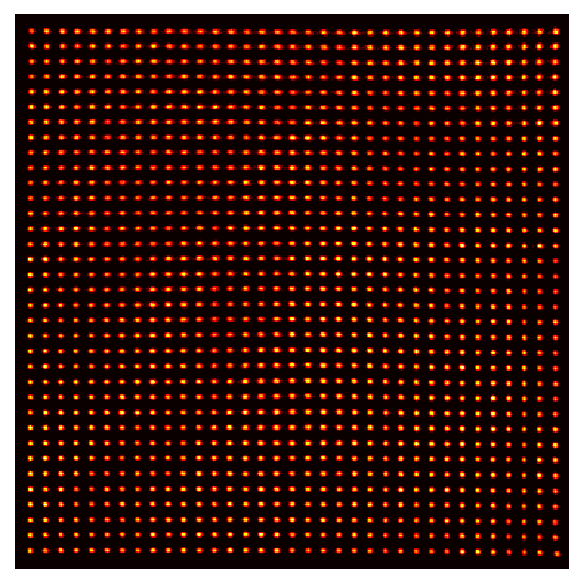
\includegraphics[width=0.4\textwidth]{Images/ica_img_20211210_full_array_hot_no_frame.pdf}
% \end{center}

%% Add \part declarations if you want, but it's not necessary
%\part{Preliminaries}

\svnidlong{$LastChangedBy$}{$LastChangedRevision$}{$LastChangedDate$}{$HeadURL: http://freevariable.com/dissertation/branches/diss-template/frontmatter/frontmatter.tex $}
% \vcinfo{} % what does this do?

%%% SOME OF THIS CODE IS ADAPTED FROM THE VENERABLE withesis.cls

% \clearpage
% \begin{center}
%   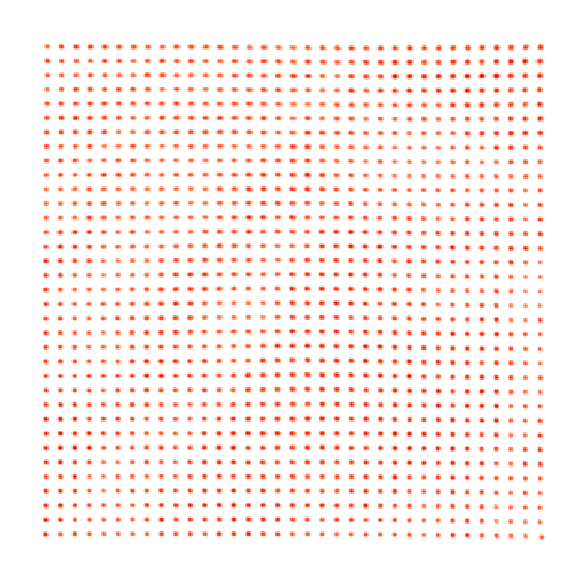
\includegraphics[width=0.4\textwidth]{Images/thesis_front_page_atom_array.pdf}
% \end{center}

% COPYRIGHT PAGE
%  - To include a copyright page use \copyrightpage
% \copyrightpage

% DEDICATION
% \begin{dedication}
% 	\emph{Please insert your dedication here.}
% \end{dedication}

%% BEGIN PAGESTYLE

%%% You can pick a pagestyle if you want; see the memoir class
%%% documentation for more info.  The default ``deposit'' option meets
%%% the UW thesis typesetting requirements but is probably
%%% unsatisfactory for making a version of your dissertation that
%%% won't be deposited to the graduate school (e.g. for web or a nice
%%% printed copy)

\chapterstyle{deposit}
\pagestyle{deposit}


% ACKNOWLEDGMENTS
\begin{acks}
% uncomment aks block in frontmatter.tex to show this

% \begin{wbepi}{David C.~Makinson (1965)}
% It is customary for authors of academic books to include in their prefaces statements such as this: ``I am indebted to ... for their invaluable help; however, any errors which remain are my sole responsibility.'' Occasionally an author will go further. Rather than say that if there are any mistakes then he is responsible for them, he will say that there will inevitably be some mistakes and he is responsible for them....

% Although the shouldering of all responsibility is usually a social ritual, the admission that errors exist is not --- it is often a sincere avowal of belief. But this appears to present a living and everyday example of a situation which philosophers have commonly dismissed as absurd; that it is sometimes rational to hold logically incompatible beliefs.
% \end{wbepi}

% Above is the famous ``preface paradox,'' which illustrates how to use the \texttt{wbepi} environment for epigraphs at the beginning of chapters.  You probably also want to thank the Academy.

Spending the majority of days over the course of six and a half years in one room in Chamberlin Hall has been a truly formative experience. The privilege of being able to work alongside so many devoted and bright peers has allowed me to learn so much in so short a time, and for that I am truly grateful. Earning this degree has been as much a team effort as an individual one, and every one of my peers here has in some way made a substantive contribution to that. Additionally, I would like to express deep appreciation for what is beyond Chamberlin Hall, namely the city of Madison. You have so much to offer, from being friendly, endlessly walkable, and filled with parks, to having no shortage of bike paths meandering out into the country. I'm going to miss it. Thanks also to my family for being encouraging and supportive of my endeavors here.

To my colleagues over the years in the Rubidium lab, or the SNAQ lab, as we have been calling it more recently, I owe you a great deal of gratitude. The experiments that have transpired in that room over the years here have kept us on our toes, often being the thorns in our collective side, but you have stuck with them and stuck with me through all of it. I would like to first thank Minho Kwon, who told me early on that keeping a good spirit was the most challenging part of grad school. Thanks also to Chris Young, whose general knowledge of science, especially entemology, never ceased to impress and entertain during long slogs in the lab. In more recent years, during the quantum network era, I would like to thank Akbar Safari for teaching me so much over the past few years and being a pivotal force in the lab. Your guidance, patience, and encyclopedic knowledge of physics -- in AMO and beyond-- has helped me immensely. To Eunji Oh-- thanks for being a great partner in the lab, always making the best of the lab catastrophy du jour. Your diligence, intellect, and ability to problem solve have really helped push things along. I'm sure you'll finish strong. To Gavin Chase, thanks for your general willingness to be a team player, and best of luck finishing your circuitous PhD. To Jihwan Moon, best of luck building up the new Cesium experiment-- make better choices than your predecessors with experiment design. To Omar Nagib-- congrats on escaping work in the lab before it had a chance to significantly slow down your progress towards the PhD. Your theory work has been exciting to follow. I would also like to thank former colleagues Kais Jooya and Yunheung Song for being dedicated partners on the short-lived trap array experiment\footnote{The project was short, and so was the trap lifetime.}.

The QPAL group turned out to be a good place for me to be for a number of reasons, not the least of which was because of the people with whom I have had the pleasure to work. I have appreciated being surrounded by clever, knowledgeable peers who are always willing to lend a hand or help stew on a problem in lab. Thanks in particular to Trent Graham, for sharing tips and tricks from your vast experience, and always being willing to help me think through a physics problem. Thanks also to Ravi Chinnarasu for letting me pick your brain on physics issues and for your help in the early days of the SNAQ project. To Jacob Scott, thanks so much for all of the time you sacrificed helping me track down ground loops in the lab. Thanks to Juan Bohorquez for always being game to escape the lab for dinner and for being my writing partner when we both started our theses. Thanks to Sam for comisserating, shooting the breeze, and providing detailed comments on an early draft of this work. There are too many other people I've crossed paths with here to name them all, but I would like to also thank in no particular order, Jake Uribe, Michael Bergdolt, Z. Alphonse Marra, Sebastian Malewicz, Xiaoyu Jiang, Chris Yip, Jin Zhang, Matt Ebert, and Isaac Scott. Finally, thanks to Mark Saffman, for affording me a generous amount of autonomy and trust in the lab, and for having high standards for my work.

My time here has not passed without being peppered with collaborations and friendships in other lab groups or departments. To Deniz Yavuz and his group, in particular, David Gold, Utku Sa\text{\u{g}}lam, and Matt Beede-- you guys have felt like my cousins in the department, and I've always enjoyed being able to walk down the hall to discuss some issue or exchange equipment. Thanks to Mikhail Kats and his group in ECE for thoughtful discussions and for weathering the storm that research often is. Thanks especially to Sanket Deshpande for all the good times. Thanks to Randy Goldsmith and his group in Chemistry for putting so much effort into the fiber cavity experiment which I had a short stint on. Thanks to Aidan Tollefson in Medical Physics for being a total copy cat and following me here after undergrad, and for all of the much needed non-physics chats and running advice.

Finally, thanks to Margaret Fortman. You've been there through thick and thin, and its crazy that we've both gotten to go through this together, from start to finish. Your companionship has been indispensible.

\end{acks}

% CONTENTS, TABLES, FIGURES
\renewcommand{\printtoctitle}[1]{\chapter*{#1}}
\renewcommand{\printloftitle}[1]{\chapter*{#1}}
\renewcommand{\printlottitle}[1]{\chapter*{#1}}

\renewcommand{\tocmark}{}
\renewcommand{\lofmark}{}
\renewcommand{\lotmark}{}

\renewcommand{\tocheadstart}{}
\renewcommand{\lofheadstart}{}
\renewcommand{\lotheadstart}{}

\renewcommand{\aftertoctitle}{}
\renewcommand{\afterloftitle}{}
\renewcommand{\afterlottitle}{}

\renewcommand{\cftchapterfont}{\normalfont} 
\renewcommand{\cftsectionfont}{\itshape} 
\renewcommand{\cftchapterpagefont}{\normalfont} 
\renewcommand{\cftchapterpresnum}{\bfseries} 
\renewcommand{\cftchapterleader}{} 
\renewcommand{\cftsectionleader}{} 
\renewcommand{\cftchapterafterpnum}{\cftparfillskip} 
\renewcommand{\cftsectionafterpnum}{\cftparfillskip} 

% \captionnamefont{\small\sffamily} 
% \captiontitlefont{\small\sffamily} 

% \renewcommand{\contentsname}{contents}
% \renewcommand{\listfigurename}{list of figures}
% \renewcommand{\listtablename}{list of tables}

\tableofcontents

\clearpage
\listoftables

\clearpage
\listoffigures

\clearpage
% NOMENCLATURE
% \begin{conventions}
% % \begin{description}
% % \item{\makebox[0.75in][l]{term}
% %        \parbox[t]{5in}{definition\\}}
% % \end{description}
% \input{conventions}
% \end{conventions}

\advisorname{Mark Saffman}
\advisortitle{Professor}
% ABSTRACT
\begin{umiabstract}
  % \textbf{FIXME:  basically a placeholder; do not believe}

\svnidlong{$LastChangedBy$}{$LastChangedRevision$}{$LastChangedDate$}{$HeadURL: http://freevariable.com/dissertation/branches/diss-template/frontmatter/abstract.tex $}
\vcinfo{}

%not great. probably rewrite

Quantum technologies are receiving great attention on a global scale, where the quantum computing market is estimated to be worth nearly 1 billion USD\cite{FortuneBusinessInsights2024} at the time of writing this. Despite tremendous progress in the industry toward prototypical devices and early attempts at showing quantum utility, there remain a number of outstanding technical challenges. State of the art quantum computers still take up substantial space, harkening back to the vacuum tube era of classical computing. Reducing the spatial requirements and improving the portability of such machines, by which we mean the ability of these machines to be operated without a team of PhD physicists and engineers on site, is an important goal if this technology is to mature.

This thesis presents some small steps toward reducing the experimental complexity of neutral atom quantum registers and quantum network nodes. Systems based on atomic qubits, as opposed to the various solid state platforms, are infamous for their room-filling Rube Goldberg machine-like apparatuses, comprised of labrynthine optical paths for a myriad of lasers, often by constructed optic by optic by tired graduate students\footnote{Often just to be rebuilt from scratch the next week, of course}. Although much of the quantum network apparatus described in this thesis can still be described in these terms, the core of the experiment is a fiber-coupled vacuum chamber containing prealigned miniature optics in-vacuo. This drastically reduces the number of components needed for launching six different laser wavelengths at our atoms as well for collecting photons from the atoms with moderate efficiency. This reduces the experimental footprint, enhances mechanical stability, and reduces the overall complexity of the constructed apparatus. This thesis details the work involved to acheive this, the unique engineering hurdles encountered, and initial characterization of the network node with cold atoms. 

Secondly, we demonstrate a method of trapping atomic qubits in a projected array of optical traps which relies only on passive optical components to generate the trapping pattern. In the same spirit as the fiber-coupled network node, this technique reduces experimental overhead required to trap an atomic register in favor of a less complex solution than the typical methods employed in our field. % needs reworking
\end{umiabstract}

\begin{abstract}
  % \textbf{FIXME:  basically a placeholder; do not believe}

\svnidlong{$LastChangedBy$}{$LastChangedRevision$}{$LastChangedDate$}{$HeadURL: http://freevariable.com/dissertation/branches/diss-template/frontmatter/abstract.tex $}
\vcinfo{}

%not great. probably rewrite

Quantum technologies are receiving great attention on a global scale, where the quantum computing market is estimated to be worth nearly 1 billion USD\cite{FortuneBusinessInsights2024} at the time of writing this. Despite tremendous progress in the industry toward prototypical devices and early attempts at showing quantum utility, there remain a number of outstanding technical challenges. State of the art quantum computers still take up substantial space, harkening back to the vacuum tube era of classical computing. Reducing the spatial requirements and improving the portability of such machines, by which we mean the ability of these machines to be operated without a team of PhD physicists and engineers on site, is an important goal if this technology is to mature.

This thesis presents some small steps toward reducing the experimental complexity of neutral atom quantum registers and quantum network nodes. Systems based on atomic qubits, as opposed to the various solid state platforms, are infamous for their room-filling Rube Goldberg machine-like apparatuses, comprised of labrynthine optical paths for a myriad of lasers, often by constructed optic by optic by tired graduate students\footnote{Often just to be rebuilt from scratch the next week, of course}. Although much of the quantum network apparatus described in this thesis can still be described in these terms, the core of the experiment is a fiber-coupled vacuum chamber containing prealigned miniature optics in-vacuo. This drastically reduces the number of components needed for launching six different laser wavelengths at our atoms as well for collecting photons from the atoms with moderate efficiency. This reduces the experimental footprint, enhances mechanical stability, and reduces the overall complexity of the constructed apparatus. This thesis details the work involved to acheive this, the unique engineering hurdles encountered, and initial characterization of the network node with cold atoms. 

Secondly, we demonstrate a method of trapping atomic qubits in a projected array of optical traps which relies only on passive optical components to generate the trapping pattern. In the same spirit as the fiber-coupled network node, this technique reduces experimental overhead required to trap an atomic register in favor of a less complex solution than the typical methods employed in our field. % needs reworking
\end{abstract}

\clearpage\pagenumbering{arabic}

%%% END STUFF TAKEN FROM WITHESIS EXAMPLE FILE


%% Now include the tex files for each chapter, like so (I put these in separate dirs): 
% note that Parts (Part I,II,etc) are added at the beginning of the chapter tex files using, e.g. \part{Conclusion}
\part{Theory and Background}\label{part:theory}
\chapter{Quantum networking with neutral Rubidium atoms}\label{ch:intro_to_qn}

% the hierarchy is 
% chapter,section,subsection,etc


\section{Intro to quantum networks}
\subsection{Distributed quantum entanglement as a resource}
Quantum entanglement is a phenomenon in which two or more systems can not be correctly described by treating the systems individually. This is equivalent to saying that the quantum state of the system is not factorable into states for each subsystem. For a system composed of subsystems $A$ and $B$ in an entangled state, e.g. two photons,
\begin{equation}
    \rho_{AB} \neq \rho_A \otimes \rho_B
\end{equation}
for two systems $A$ and $B$ where $\rho$ is a Hermitian matrix representing the density operator which gives the state, and the right-hand-side (RHS) represents a product state.
In many cases, the entanglement applies only to one particular degree of freedom, such as the spin state of an atom or the polarization of a photon, whereas the other degrees of freedom remain separable and distinguishable, thus they can be factored out of the overall state. However, entanglement can also involve multiple degrees of freedom, such as both the polarization and frequency of photons, which is referred to as hyperentanglement.

In addition to being an active area of fundamental research, quantum entanglement is also a useful resource in applications such as quantum sensing. Typical quantum sensing schemes rely on measuring the phase between two quantum states, for example using a Ramsey-type interference experiment. For such applications, certain quantum entangled states can show advantage over product states inputs, e.g. owing to a phase which evolves more rapidly than for an unentangled system. Two common states of interest for quantum sensing are GHZ states and N00N states:

\begin{align}
    \ket{\psi_{\text{GHZ}}} &= \frac{1}{\sqrt{2}} \left(\ket{0}^{\otimes n} + \ket{1}^{\otimes n}\right) \\
    \ket{\psi_{\text{N00N}}} &= \frac{1}{\sqrt{2}} \left( \ket{n0} + \ket{0n} \right)
\end{align}
    
Another convenient albeit mysterious attribute of quantum entanglement is that it can be created between widely separated systems, including systems which have never directly interacted. Indeed, entanglement has been generated between photons across 100s and even 1000 km \cite{Neumann2022, Yin2020}. This opens up the door for long-range sensing, such as a network of quantum clocks\cite{Kómár2014}, as well as a network of eaves-drop proof secure communication channels. Moreover, across shorter distances, such distributed entanglement may be an enabling technology for scaling quantum computers, using a network of quantum processor modules\cite{Monroe2014modular}. Some of these applications will be discussed in more detail throughout this thesis.

\section{Quantum networking with neutral atom qubits}

A quantum network can be roughly defined as any system of communication channels in which quantum mechanics plays a role to accomplish some non-classical behavior. For the purpose of this thesis, we will usually take a quantum network to imply a more restricted definition, in which $N\geq2$ spatially-separated systems containing matter qubits acting as quantum memory are interconnected by quantum entanglement. The most rudimentary architecture within this definition is two spatially separated two-level systems sharing entanglement, say two atoms with entanglement between their hyperfine states-- the exact architecture of interest to this thesis. It is worth noting that despite its simplicity, such a system can still be used to demonstrate several fundamental features and important building blocks for quantum sensing, quantum key distribution, and distributed quantum computing\cite{main2024, drmota2024, Langenfeld2021}.

To date, distributed or remote entanglement has been generated with many different physical platforms, including but not limited to photons, neutral atoms, ions, nitrogen-vacancy centers in diamond, and superconducting qubits. It is still an open question which system(s) will prevail for useful quantum applications such as distributed quantum processing and sensing. However, as this thesis is concerned with remote entanglement between neutral atoms, we will focus on the advantages and disadvantages of that particular platform at present.

Neutral atoms are renowned in the world of qubits for their inherently identical properties between copies of the same atom, long coherence times, and the ability to interact with electromagnetic fields in a variety of different ranges, from microwave to optical. Moreover, techniques for controlling them are relatively mature thanks to decades of progress in the field and technological advancements, e.g. lasers.  However, no platform is without its downsides. Notably, neutral atoms confined in optical potentials typically remain trapped for only tens of seconds\cite{Schymik2021}, necessitating costly time to reload atoms. This is in contrast with solid state qubits which persist indefinitely and ions which can remain trapped for days in deep traps even with room temperature vacuum systems\cite{Wu2021}.

For quantum networking in particular, neutral atoms possess several key attributes. It is well established that atoms make excellent clocks and quantum sensors for a variety of quantities of interest: electric and magnetic fields, acceleration, and gravitational red-shifts \cite{Kumar2017, d’ArmagnacdeCastanet2024, Bothwell2022}, to name just a few. Moreover, neutral atoms are emerging as a top contender for quantum computing, owing to a relatively  straightforward path to scalability of optical trap arrays \cite{Huft2022, manetsch2024, Pause2024}, high-fidelity gates using architectures based on either fixed atom arrangement \cite{radnaev2024} or flexible qubit connectivity through atom transport\cite{Evered2023}. Thus, it is natural to pursue linking these extant technologies as the quantum IoT ecosystem develops.

?? put the network of quantum registers image from my talks/posters here?

\subsection{Establishing remote entanglement}\label{sec:reg}

Remote entanglement between a pair matter qubits is implemented by intermediate entanglement generation between one or both matter qubits with a flying qubit, or photon. In one class of entanglement schemes, each qubits, say, an atom, is prepared in such a way as to emit a single photon with which it shares entanglement. When a photon from each atom is collected with appropriate optics, the paths of the photons allow them to interfere, entangling the photonic part of the state of the system of atoms and photons. Finally, a measurement is made on the photons which projects entanglement onto the atoms. This is an example of entanglement swapping (?? cite). This scheme is probabilistic as the photons are not collected with unit success probability, but successful entanglement is heralded by the photon detection event.

A second class of remote entanglement schemes involves so-called direct transmission, in which only one atom is entangled with an emitted photon, which is then sent directly to the other atom to be absorbed. This scheme does not always include a heralding event, and can suffer from poor interaction between the photon and receiving atom unless a cavity is used. For the experiment developed for this thesis, the first method of entanglement generation above will be the one of interest.

%the chapters and section are not in the best order. this could go before the "establishing remote entanglement section", and all of the sections before "A remote entanglement protocol with Rb" could go in the intro to quantum networks section, with Quantum networking with neutral atom qubits as the final subsection in that section. the new section would be remote entanglement with rb atoms, and the atom-atom rate could be demoted to a subsection   
\subsection{Quantum networks for distributed processing}

lots of recent interest, yada yada, proposal by Jeff Thompson, Vuletic, us, review by Covey, \cite{Thompson2024, sinclair2024, Covey2023, Young2022}, basic demonstration with ions in Lucas group, could be used for lattice surgery \cite{Horsman2012}

%now we get specific
\subsection{A remote entanglement protocol with $^{87}$Rb atoms}

The quantum networks described in this thesis use $^{87}$Rb as the matter qubit in each network node involved in entanglement distribution. This choice was made in part to due to its convenient level structure for our choice of entanglement between the spin states of the atom and polarization states of the emitted photon. In what follows, we will describe the remote entanglement protocol in detail.

The remote entanglement generation protocol can be coarsely broken into three chunks. First, a cooled and trapped communication atom at each node is optically pumped into $\ket{5S_{1/2},F=1,m_F=0}$ (Fig. (\ref{fig:entanglement_generation_steps})). Second, the atoms are excited with a $\pi$ pulse to $\ket{5P_{3/2},F=0,m_F=0}$. The atom then undergoes spontaneous emission into three possible decay channels, emitting a photon with either circular polarization $\sigma_{\pm}$ or linear $\pi$. By choosing a quantization axis aligned along the optics which collect the photon and coupling the emission into a single mode fiber, we can restrict the collected photons to only those with circular polarization. This is because the $\pi$-polarized dipole pattern destructively interferes along the quantization axis. Owing to the indistinguishability of the two $\sigma$ decay channels, the collection of a photon results in an atom-photon entangled state given by
\begin{equation}\label{eq:atomphotonstates}
    \ket{\psi^+}=\frac{1}{\sqrt{2}}\left(\ket{m_F=1, \sigma_+}+\ket{m_F=-1,\sigma_-}\right)
\end{equation}
where the phase of the state is fixed by a Clebsch-Gordon coefficient for the decay. Repeated attempts done in parallel to create this state at both nodes until a photon from each node is collected on the same attempt. When this occurs, a joint measurement is done on the photons, which can project the remaining two-atom state into one of two Bell states,
\begin{equation}\label{eq:atomatomstates}
    \ket{\Psi^{\pm}} =\frac{1}{\sqrt{2}}\left(\ket{1,-1}\pm\ket{-1,1}\right)
\end{equation}
with a maximum success probability of $1/2$. The scheme described here was first demonstrated in \cite{Hofmann2012}

\begin{figure}[!ht]
    \centering
    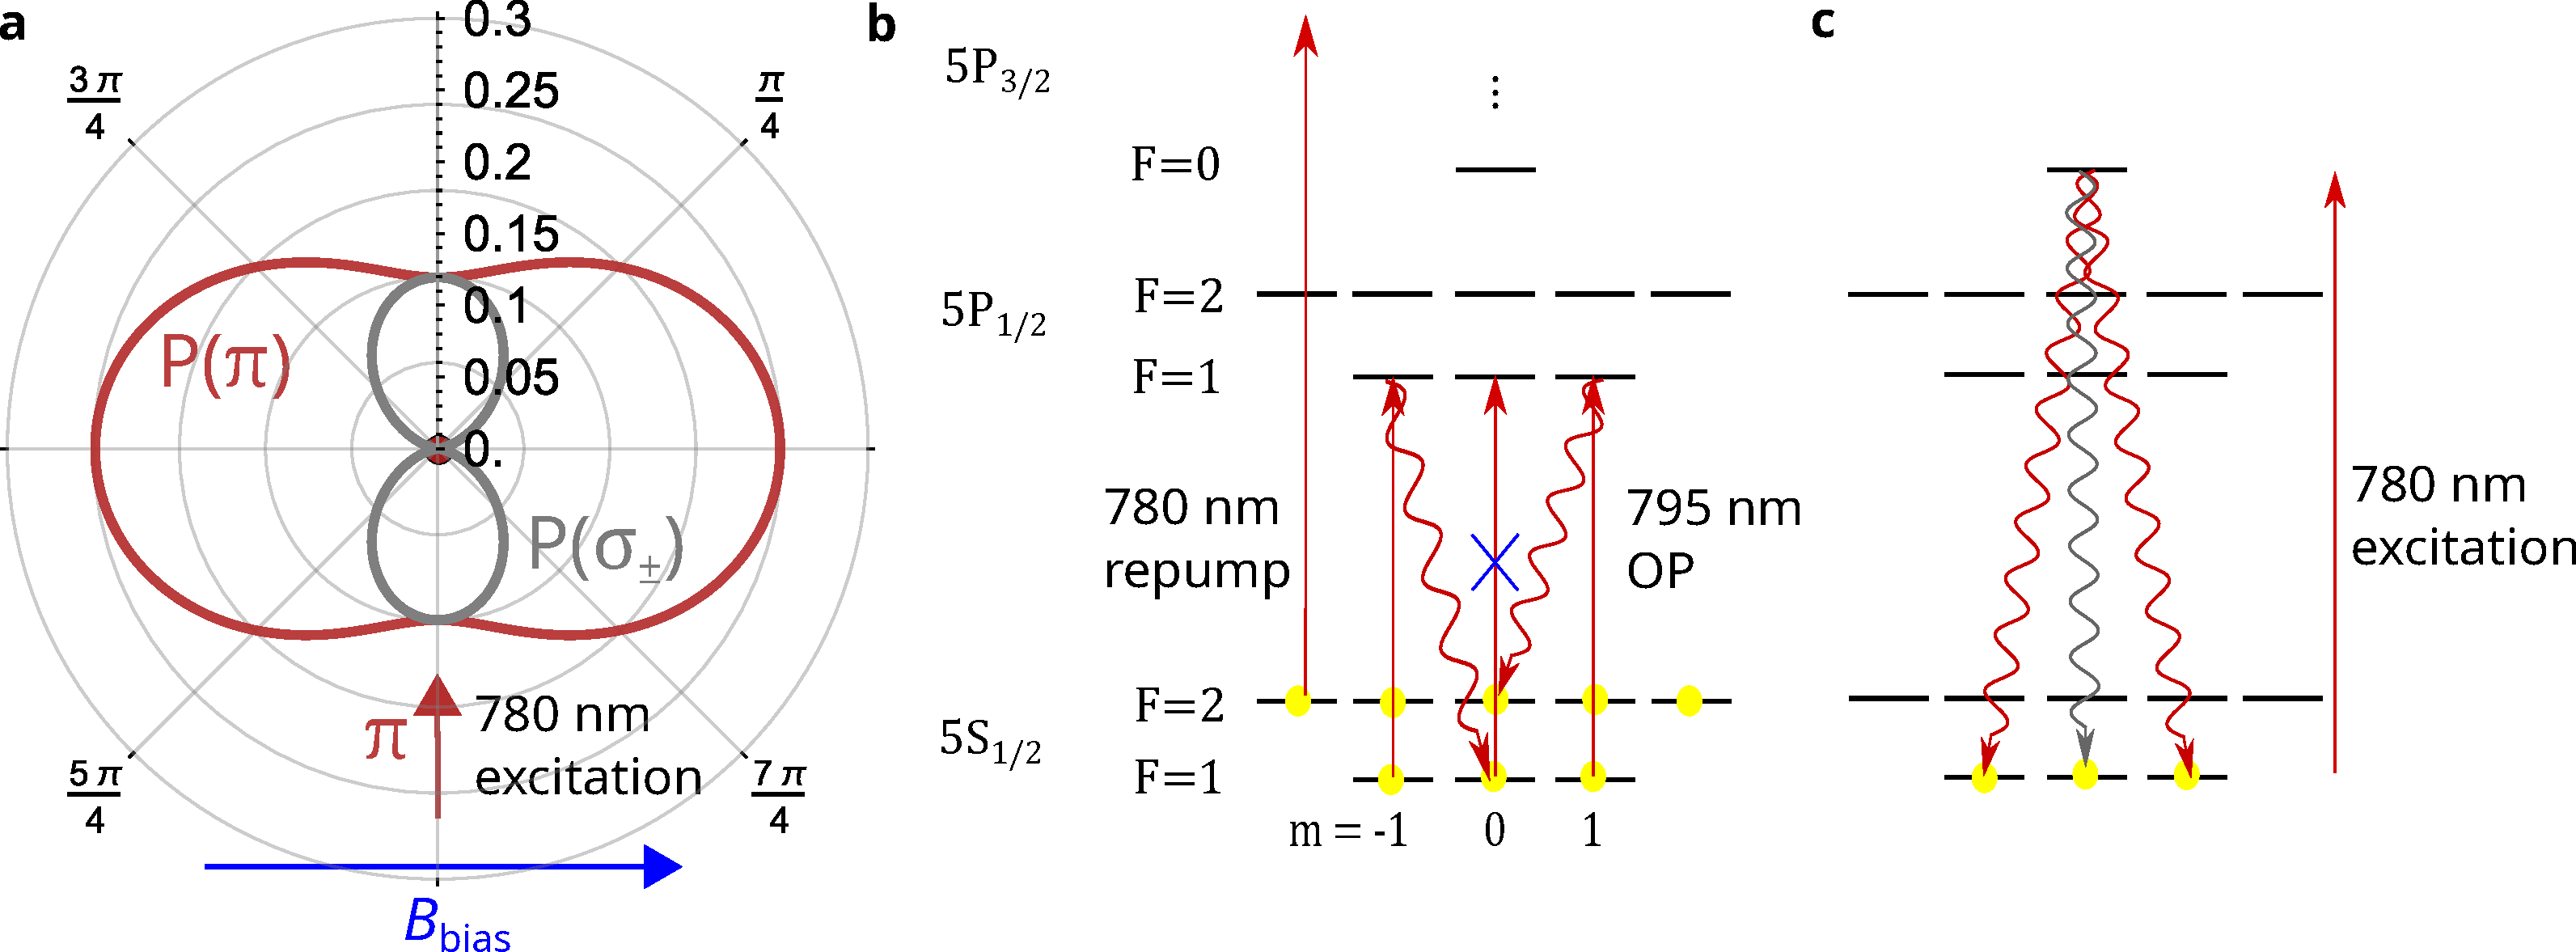
\includegraphics[width=0.9\textwidth]{Images/rb87_atomphoton_entanglement_and_photon_emission_pattern2.pdf}
    \caption{The atom-photon entanglement generation protocol. \textbf{a} The dipole emission pattern of the atom, oriented with the quantization axis defined by a magnetic field $B_{\text{bias}}$ aligned to the optical axis of the photon collection optics. \textbf{b} The communication atom at each node is optically pumped into $\ket{5S_{1/2},F=1,m_F=0}$, after which \textbf{c} the atom is excited with a $\pi$ pulse to $\ket{5P_{1/2},F=0,m_F=0}$, resulting in the creation of an atom-photon entangled state (see text).}
    \label{fig:entanglement_generation_steps}
\end{figure}

% \subsection{Integrating quantum processing arrays with network nodes}
\section{Atom-atom entanglement rate}\label{sec:entanglementrate}

The entanglement protocol described above is probabilistic and requires many attempts per heralded remote entanglement event, predominantly limited by the efficiency of the photon collection optics. It is important to estimate the expected remote entanglement generation (REG) rate, as this will affect what the entanglement resource can be used for. For example, if the REG rate much greater than the decoherence rate of the entangled state, we can generate many entangled pairs in succession, which may be a requirement for some entanglement purification protocols as well as quantum sensing.

The per-attempt success probability of REG, i.e. atom-atom entanglement, is given simply by
\begin{equation}
    P_{\text{aa}} = \frac{1}{2}P_{\text{ap}}^2
\end{equation}
where $P_{\text{ap}}$ denotes the one-node atom-photon entanglement success probability and the factor of $1/2$ results from only two out of four Bell states being able to be distinguished by the photonic Bell state measurement. $P_{\text{ap}}$ is limited by the photon collection efficiency of per excitation attempt $\eta_{\text{col}}$ and the detection efficiency $\eta_{\text{det}}$. All losses from optical alignment, finite transmission through optical elements including absorption in optical fiber, and detector efficiency can be lumped into these two quantities, so we can write 
\begin{equation}
    P_{\text{aa}} = \frac{1}{2}\left(\eta_{\text{col}}\eta_{\text{det}}\right)^2
\end{equation}
where it has been assumed that the collection and detection efficiency are the same for each node. Additional losses such as imperfect success probability in initializing the atom state and exciting it have been ignored, but these could be accounted for by including them in $\eta_{\text{col}}$.

The rate of REG depends on the atom-photon entanglement attempt rate and the duty cycle of the attempt loop (Fig. (\ref{fig:REG_loop})), such that the average REG rate is given by
\begin{equation}\label{eq:Raa}
    R_{\text{aa}} = \eta_{\text{duty}}R_{\text{attempt}}P_{a   a} = \bar{R}_{\text{attempt}}P_{\text{aa}}
\end{equation}
where $\bar{R}_{\text{attempt}}$ is the average attempt rate. The duty cycle $\eta_{\text{duty}}$ is to some extent platform dependent. For example, neutral atoms can occasionally be lost from the trap either through heating during the excitation loop or by collisions with background atoms, necessitating a break in the loop for reloading an atom which can take 100s of ms. For platforms such as ions and NV centers this kind of break is not needed. It is worth noting however that the REG rate reported in literature does not always take into account the duty cycle of the excitation loop, such as in \cite{Young2022}, such that the reported rate is really max rate rather than the average rate. Whether this distinction is important is likely application dependent, but it is clear that a high rate REG loop broken up by large amounts of downtime could be severely limiting.

\begin{figure}[!ht]
    \centering
    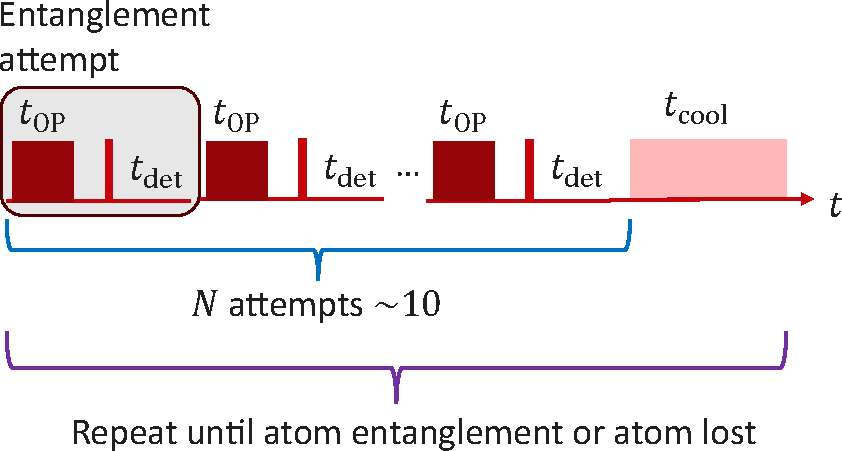
\includegraphics[width=0.5\textwidth]{Images/entanglement_attempt_loop.pdf}
    \caption{The remote entanglement generation loop.}
    \label{fig:REG_loop}
\end{figure}

The attempt rate $R_{\text{aa}}$ can be estimated given the duration of the different elements of the experiment sequence together with assumptions for the atom lifetime in the trap and heating rate. The entanglement attempt loop sequence in shown in Fig. \ref{fig:REG_loop}, and consists of optical pumping and excitation phases interspersed with Doppler re-cooling to alleviate atom heating, as well as atom reloading triggered by the absence of an atom signal during re-cooling. To write down the attempt rate, we first define the following quantities:
\begin{align}
    N_{\text{total}} &= \frac{1}{P_{\text{aa}}} \\
    N_{\text{epoch}} &= \frac{N_{\text{total}}}{N_{\text{series}}}.
\end{align}
The first line gives the mean number of tries per REG success, and second gives the number entanglement "epochs", where one epoch is defined as a sequence of entanglement attempts followed by one Doppler re-cooling phase. $N_{\text{series}}$ is the number of entanglement attempts (optical pumping follwed by excitation pulse) we can do in series with re-cooling, i.e. the number of attempts per epoch. Using these definitions, the mean time per remote entanglement success during the attempt loop is 
\begin{equation}
    t_{\text{aa}}=\frac{t_{\text{aa}}^{(\text{loop})}}{\eta_{\text{duty}}}=\frac{1}{\eta_{\text{duty}}}N_{\text{epoch}}\left(N_{\text{series}}\left(t_{\text{OP}} + t_{\pi} + t_{\text{det}}\right) + t_{\text{cool}}\right)
\end{equation}
where the subscripted times denote the optical pumping, $\pi$-pulse excitation, detection, and Doppler re-cooling durations. This gives the REG rate that appears in Eq. (\ref{eq:Raa}) as $R_{\text{aa}} = \eta_{\text{duty}}/t_{\text{aa}}^{(\text{loop})}$. For realistic parameters (see Table \ref{tab:entanglement_steps}), we can compute $P_{\text{aa}}$ and $R_{\text{aa}}$.

\newpage
\begin{sidewaystable}
% \begin{table}[h!] % too wide
    \centering    
    \begin{tabular}{llll}
        \hline Operation & Label & Duration & Success probability \\
        \hline (a) Entanglement generation: & & & \\
        1- prepare MOT, load into dipole trap & $t_{\textrm{load}}$ & 500 ms & $>0.99$ \\
        2- pump to $5 s_{1 / 2}\ket{1,0}$ & $t_{\textrm{OP}}$ & $6 \mu \mathrm{~s}$ & $>0.99$ \\
        3- $\pi$-pulse to $5 p_{3 / 2}\ket{0,0}$ & $t_\pi$ & 30 ns & $>0.99$ \\
        4a- atomic decay, record and process photon clicks & $t_{\text {det }}$ & $1 \mu \mathrm{~s}$ & 1 \\
        4b- cool atom if proper coincidence is not registered after $N_1=10$ cycles & $t_{\textrm{cool}}$ & $100 \mu \mathrm{~s}$ & $>0.99$ \\
        (b) Entanglement verification: & & & \\
        5- map atomic qubit states $\ket{1,1} \rightarrow \ket{2,1}$ with $\mu$-wave $\pi$-pulse & $t_{\textrm{pw}}$ & $50 \mu \mathrm{~s}$ & $\sim 0.99$ \\
        6- atomic qubit rotation with $\mu$-wave $+\mathrm{RF} \pi / 2$ pulse & $t_{\mathrm{m}}$ & $500 \mu \mathrm{~s}$ & $\sim 0.98$ \\
        7- non-destructive atomic state measurement & $t_{\textrm{cool}}$ & 3 ms & $\sim 0.94$\cite{Kwon2017} \\
        8- cool atom to maintain localization in trap & $100 \mu \mathrm{~s}$ & $>0.99$ \\
        \hline
    \end{tabular}
    \caption{Entanglement generation and tomography operations and estimates of their durations, adapted from \cite{Young2022}.}
    \label{tab:entanglement_steps}
% \end{table}
\end{sidewaystable}
\newpage

Although we can reuse atoms by re-cooling between successive entanglement attempts, eventually an atom will be lost due to a collision with background atoms. We can expect an average number of entanglement events before needing to reload an atom given by 
\begin{equation}
    N_{\text{aa}} = \frac{\tau_{\text{trap}}}{t_{\text{aa}}}
\end{equation}
where $\tau_{\text{trap}}$ is the lifetime of the atom in the dipole trap. This can be though of as an upper bound, as experiments in which the entanglement is used for something, e.g. for sensing, will likely need to reload atoms more often. State-of-the-art experiments have shown trap lifetimes of 1000s of seconds in cryogenic environments \cite{Schymik2021}, and typically $\sim10$ s at room temperature using two-chamber systems \cite{Graham2022}. However, for the experiment described in this thesis where the MOT is loaded from a background vapor, $\tau_{\text{trap}}$ is around 2 s.

\subsection{Link efficiency}
Another important quantity of interest for generating distributed entanglement is the link efficiency, given by the ratio of the REG rate to the entangled state decoherence rate, or equivalently the coherence time over the mean time per REG:
\begin{equation}
    \eta_{\text{link}} = \frac{R_{\text{aa}}}{\gamma_{\text{coh}}} = \frac{T_2^*}{t_{\text{aa}}}
\end{equation}
If we imagine a two-node network which can only create entanglement pairs in series, $\eta_{\text{link}}=1$ would imply that an entangled state has decohered by the time a subsequent state can be created. To date, $\eta_{\text{link}}>1$ has been out of reach for many experimental demonstrations, as shown in Fig. \ref{fig:covey_link_eff}.

\begin{figure}[!ht]
    \centering
    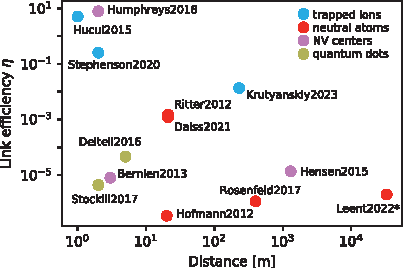
\includegraphics[width=0.7\textwidth]{Images/covey_link_efficiency.pdf}
    \caption{Link efficiency for rudimentary quantum  networks vs the node separation across different platforms, reproduced from \cite{Covey2023}}
    \label{fig:covey_link_eff}
\end{figure}

\subsection{Photon collection - optical cavity vs free-space}
% could mention assumption of negligible dark rates, then lift this assumption later.
\subsection{Experiment repetition rate}
\section{Entanglement fidelity}
\subsection{Dominant contributions}
% dark counts effect fidelity and quantum efficiency effect the rate, 
% but I discuss both effects here

There are multiple sources which contribute to the infidelity of a remote entangled state, some of which arise from infidelity sources for the atom-photon entanglement state at each node, and some of which are related specifically to the atom-atom state. TThere are several sources which go over the main points in detail, and I will not attempt to repeat this here. An overview of infidelity estimates specific to the entanglement scheme with $^{87}$Rb presented here, including effects which arise if photons are collected with a cavity rather than free-space optics, is given in\cite{Young2022}. I will go over some of these, but only in brief, as they are beyond the concern of the scope of the experimental results presented in this thesis.

Sources of infidelity specific to the creation of the atom-photon entangled state include collecting photons of unwanted polarization, dephasing of the atomic qubit, and off-resonant excitation. The latter two are essentially negligible, but the polarization has to be carefully controlled. As there are three decay channels from $F=0, m=0$ (Fig. (\ref{fig:entanglement_generation_steps}c)), and we only want a state which includes the $\sigma$-polarized components of the emission, it is important not to collect the $\pi$ component. This is accomplished if the optical collection axis coincides with the quantization axis set by a magnetic bias field, and the collected photons are coupled into a single mode fiber.

Both the atom-photon and atom-atom entanglement fidelity are affected by dark counts from the dark detector, which should be negligible. For those used in the experiment described (Laser Components COUNT NIR), the rate is 50 s$^{-1}$, which corresponds to a mean of $5\cdot 10^-7$ dark counts in a 100 ns collection window, compared to odds of order $\sim$0.05 of detecting a photon from the atom -- a signal to noise of $10^5$.

Multi-photon scattering is not a problem for our entanglement protocol, if the bias field is set correctly as discussed above, as only $\pi$-polarized emission back into $\ket{F=1,m=0}$, which is not collected, can lead to a second excitation event during the excitation pulse. Put another way, detection of a photon implies $\sigma$-polarization, such that amplitude for re-excitation is projected to zero. The re-excitation process can, however, lead to jitter in the arrival time of photons which effects the contrast of interference of photons from each node, but this is expected to be a small effect.

Mismatch in temporal, or equivalently frequency, overlap of photons from both nodes at the Bell state analyzer will degrade the atom-atom entanglement fidelity, scaling with the overlap of the wavepackets in time. This mismatch can be caused by differences in the arrival time of photons, as well as differences in their carrier frequencies or bandwidths. The former can be adjusted through the experimental control sequence timing in software and by adjusting cable and optical path lengths. The bandwidth of the photons is determined by the atomic linewidth. Any difference in carrier frequency of photons is determined by the bias field at the atoms which sets the quantization axis, and it is imperative that this difference is small compared to the transition linewidth. Imagining the overlap of the photons in frequency space is helpful for having an intuitive foothold. For a bias field of order $\sim1$ G, there will be a relative shift $\Delta$ of order $\sim2\pi\times1$ MHz between $\sigma_+$ and $\sigma_-$ photons due to the hyperfine Zeeman shifts, which is comparable to the $6$ MHz linewidth of the $5P_{3/2}$ states. This will lead to reduced Hong-Ou-Mandel contrast, but contrast can be recovered by limiting the detection window to be $< 2\pi/\Delta$, which is satisfied with a detection window of $\sim100$ ns. This arises from the time-frequency uncertainty relation for the measurement.

\subsection{Smaller effects}
\subsubsection{Polarization change from parabolic mirror}

Polarized light reflected from a surface will in general accrue a phase shift and reduction in amplitude, both of which depend on the angle of incidence and whether the polarization is perpendicular to the surface (S-polarized) or parallel to the surface (P-polarized). Both of these effects will lower the fidelity of our atom-photon entangled state, which uses a circular polarization encoding, but we will show that this is not expected to be a significant source of infidelity.

From \cite{fowles1989introduction}, the reflection amplitudes for S- and P-polarized light at a vacuum-metal boundary are given by
\begin{align}
    r_s &= \frac{\cos(\theta)-n\cos(\phi)}{\cos(\theta)+n\cos(\phi)} \\
    r_p &= \frac{-n\cos(\theta)+\cos(\phi)}{n\cos(\theta)+\cos(\phi)}
\end{align}
where $\phi = \sin^{-1}(\theta/n)$, $\theta$ is the angle of incidence, and $n$ is the complex index of refraction. The parabolic mirror used in the experiments discussed here is coated with silver, for which $n=0.033687+i 5.4208$ for 780 nm light.

Circularly polarized light, e.g. right-handed, can be written as
\begin{equation}
    \textbf{E}_{\textrm R} = E_0 \hat{e}_{\textrm p} + i E_0 \hat{e}_{\textrm s}
\end{equation}
where the $\hat{e}_{\textrm i}$ are unit vectors. After reflection, this becomes
\begin{equation}
    \textbf{E}_{\textrm R} = E_0 r_{\textrm p} \hat{e}_{\textrm p} + i E_0 r_{\textrm s} \hat{e}_{\textrm s}.
\end{equation}
We can now compute the fidelity of the reflected state to the input state in terms of the angle of reflection. Light emitted from an atom trapped at the focus of the parabolic mirror will be incident on the mirror at some angle $\theta_i$ w.r.t. the surface normal for a given emission angle $\theta$ from the optical axis. Because the reflected rays are parallel to the optical axis for an emitter at the mirror focus, $\theta_i=\theta/2$. The maximum angle is related to the clear aperture (CA) radius $\rho_{\textrm CA}$ by 
\begin{equation}
    \theta_{\textrm CA} = \tan^{-1}
    \left(\frac{\rho_{\textrm CA}}{f-\rho_{\textrm CA}^2/(4f)}\right)
\end{equation}
where $f=5.26$ mm is the mirror focal length. Finally, including a weighting function $f(\theta)$ for the emission intensity pattern, we have the fidelity of the reflected polarization state to the input state given by
\begin{equation}
    \mathcal{F} = \frac{\int_0^{ \theta_{\textrm CA}} \left|\frac{1}{2}(\hat{e}_{\textrm p} + i \hat{e}_{\textrm s})\cdot(r_{\textrm p}(\theta') \hat{e}_{\textrm p} - i r_{\textrm s}(\theta') \hat{e}_{\textrm s})\right|^2 f(\theta') d \theta'}{\int_0^{ \theta_{\textrm CA}} f(\theta')  d\theta'}.
\end{equation}
For unpolarized emission, the intensity pattern has no $\theta$ dependence so $f(\theta)=1$, resulting in $\mathcal{F}=0.99544$. We expect a marginal increase for emission which is less likely at large $\theta$, where the angle of incidence, and consequently the fidelity reduction, is more appreciable. For $\sigma$ emission with the quantization axis along the mirror, $f(\theta)=1+\cos^2(\theta)$ up to a numerical prefactor, and $\mathcal{F}=0.99545$, which is a negligibly higher than for uniform emission. We can conclude that the action of reflection from the high NA mirror does not contribute substantially to infidelity of the atom-photon Bell state.

% \subsubsection{Raman scattering in optical fibers}

% Does this matter at all?


% \include{Chapters/Ch2}
\part{Experiment}\label{part:experiment}
\chapter{Quantum network apparatus design}\label{ch:nodes}
% the hierarchy is 
% chapter,section,subsection,etc

An outstanding technical challenge for cold atom technologies, including but not limited to quantum networks and processors, is reducing the footprint of these often space-consuming apparatuses. Building more compact cold atom science platforms is of both academic and potential commercial interest, and our implementation is one of several demonstrations to date. These include 3D printed optomechanics and vacuum chambers\cite{madkhaly2021performance}, laser beam delivery with photonic integrated circuits\cite{isichenko2023photonic}, and fiber-coupled vacuum chambers with grating-based MOTs\cite{lee2022compact}. The approach we present here makes use of relatively small bulk optics which are pre-aligned and placed in the UHV chamber and connected to by fiber optic feedthroughs, making for a plug-and-play quantum testbed. The design and construction procedure for our apparatus is outlined in the remainder of this chapter.

\section{Quantum Network Node Design}
\subsection{On-chip optical architecture}

Cold atom experiments often require on the order of ten different laser beams directed into a vacuum chamber, each having optics to tune the direction, beam size, polarization; and optics for photon collection for state readout. In this work, we present a compact architecture in which light is brought into and out of the vacuum system by optical fiber feedthroughs and the light is sent to and collected from the atoms using in-vacuum optics. 
%A schematic of the apparatus is shown in Fig. \ref{fig:network_node_apparatus_schematic}.

% \begin{figure}[!ht]
%     \centering
%     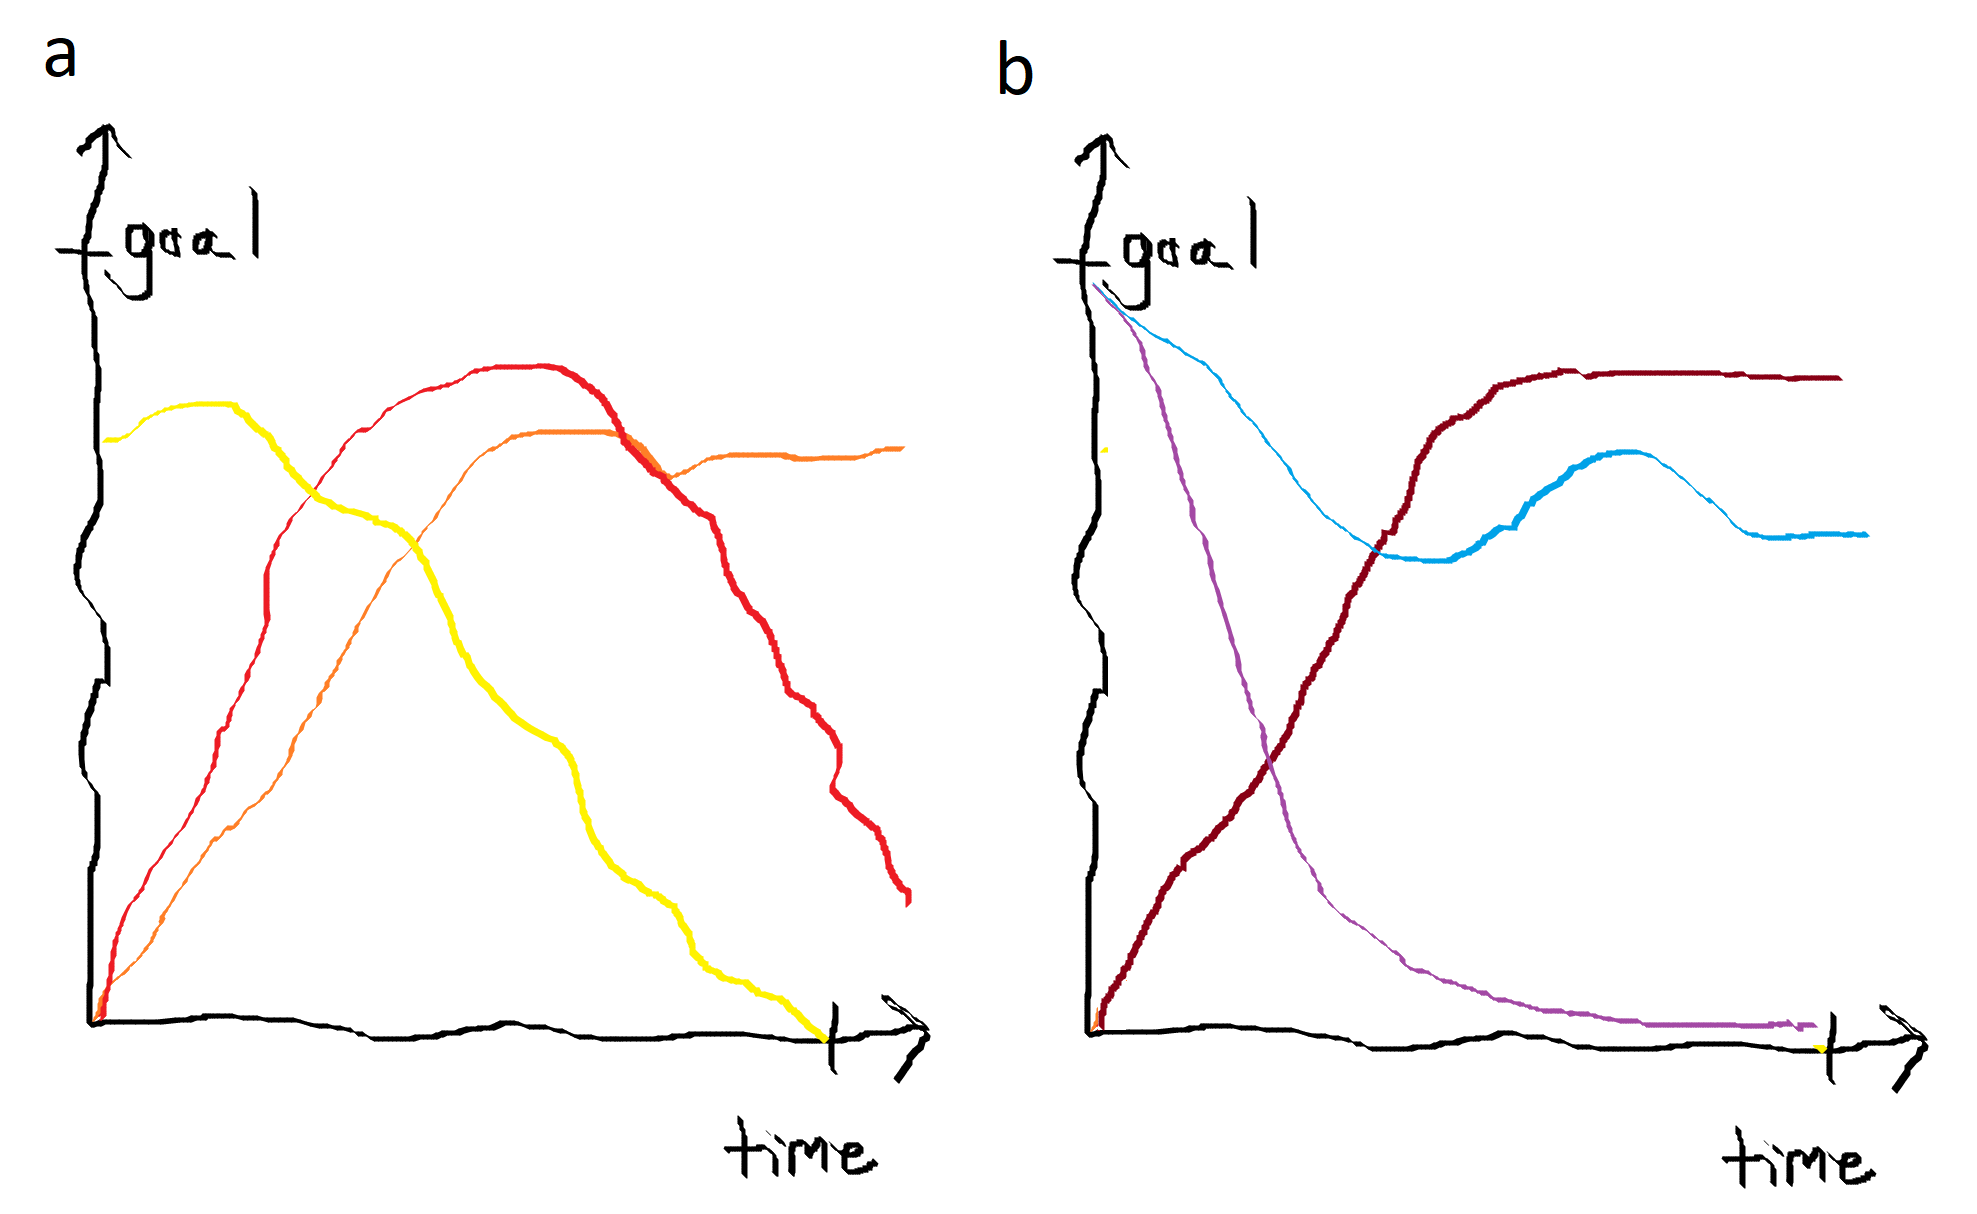
\includegraphics[width=0.45\textwidth]{Images/fig_coming_soon.png}
%     \caption{A schematic of the apparatus}
%     \label{fig:network_node_apparatus_schematic}
% \end{figure}

The in-vacuum optics are installed on a custom substrate  machined out of Macor. Macor was chosen for its low thermal expansion, mechanical strength, and ability to be machined easily using common tools such as a Dremel. This last point proved important, as it provided some insurance against some unforeseen mechanical conflicts during optical assembly. The Macor substrate, henceforth referred to as either bridge or chip, interchangeably, was designed to accommodate different optical modules consisting of bulk optics which map the light from fiber to free space beams and set the polarization. The layout of the optics for the first version of the quantum network node is shown schematically in Fig. (\ref{fig:optical_chip_design}) Each optical module, described in detail in the following sections, was individually assembled then aligned and glued to the bridge using low-outgassing epoxy. 

\begin{figure}[!ht]
    \centering
    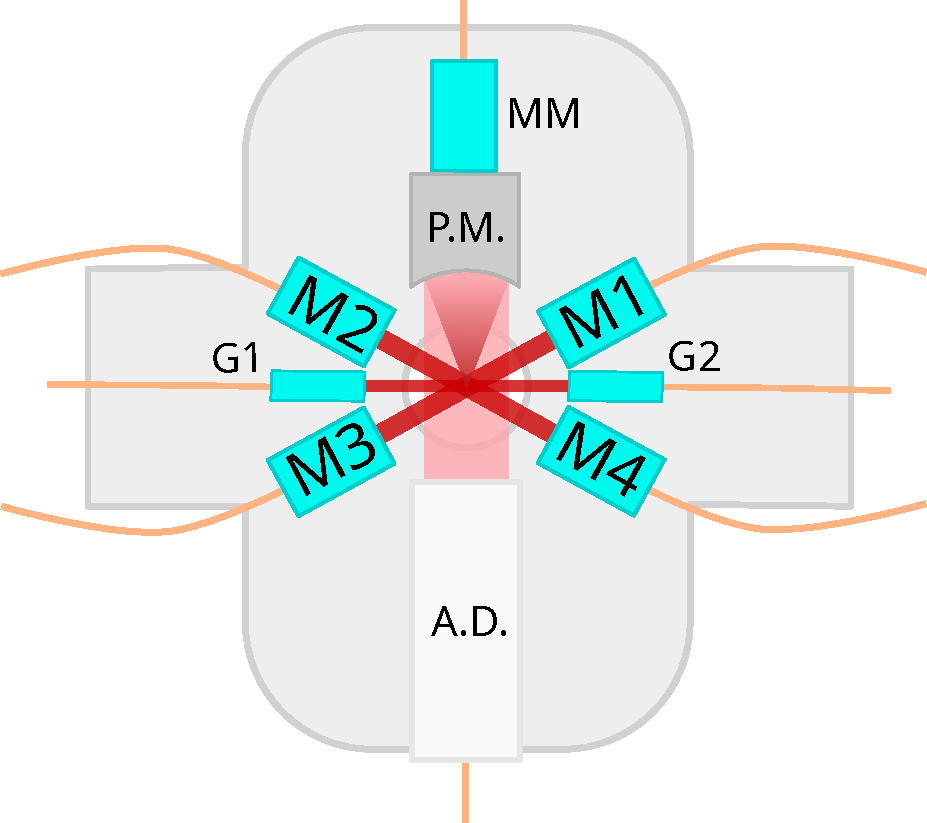
\includegraphics[width=0.45\textwidth]{Images/optical_chip_schematic.pdf}
    \caption{A simplified illustration of the layout of optical modules on the Macor bridge for the first version of the quantum network node. The modules M1-M4 (MOT 1 - MOT 4 in the text) produce the four MOT arms in a plane parallel to the bridge, G1 and G2 (GRIN 1 and GRIN 2 in the text) produce beams for optical pumping and excitation for Bell state preparation, P.M. is the parabolic mirror, and A.D. houses an achromatic doublet. In reality, A.D. and P.M. are a single optical module, but are shown separately here for clarity. MM couples light which passes through a central hole in the parabolic mirror and then a polarizer into a multimode fiber. Each module is interfaced with a polyamide coating optical fiber (orange lines), which allows coupling  light from outside the vacuum system. See Sec. \ref{sec:science_optics} for more details on the optical modules.}
    \label{fig:optical_chip_design}
\end{figure}

\subsection{Vacuum system design}
%An illustrative cross-section of the quantum network node UHV system is shown in Fig. \ref{fig:vacuum_cross_section}. 

The vacuum system consists of a custom science chamber in which the optics live, a valve and bellows to store an atomic ampule, two ion pumps (Edwards 10S TiTan), and valves for pumping down the system. 
\begin{figure}
    \centering
    \includegraphics[width=0.9\textwidth]{Images/chamber_is_open_and_shut.pdf}
    \caption{The custom two piece 6" flange-like vacuum chamber for one of the quantum network nodes. a) The brain and spinal cord of the quantum node being strung through its head (optical chip, fibers, and bottom of the chamber, respectively). Note the Kimball Physics Groover Grabbers and copper shims used for mounting the so-called optical chip. b) The optical chip in the chamber with the top window attached.}
    \label{fig:vacuum_chamber_imgs}
\end{figure}

The custom stainless steel chamber (MDC Precision) which houses the optical chip is modeled in the fashion of a pair of 6" Conflat flanges, furnished with fused silica view ports on each side for external optical access (Fig. \ref{fig:vacuum_chamber_imgs}). The view ports are AR coated on both sides for 400-1100 nm and the thickness of each was chosen so as to cancel optical aberrations when used with existing custom objective lenses (JenOptik) used in our group. The Macor chip holding the optics mounts into the chamber with the help of two Kimball Physics Groove Grabbers (6", Reverse) which mount to the inner wall of the lower half of the science chamber. The chip is situated such that the plane defined by the axes of the optical beams on the chip, and hence the region where an atom will be trapped, is equidistant from each window. See the mechanical drawing in Appendix \ref{ch:mech_drawings} for the full dimensions of the science chamber.

\begin{figure}
    \centering
    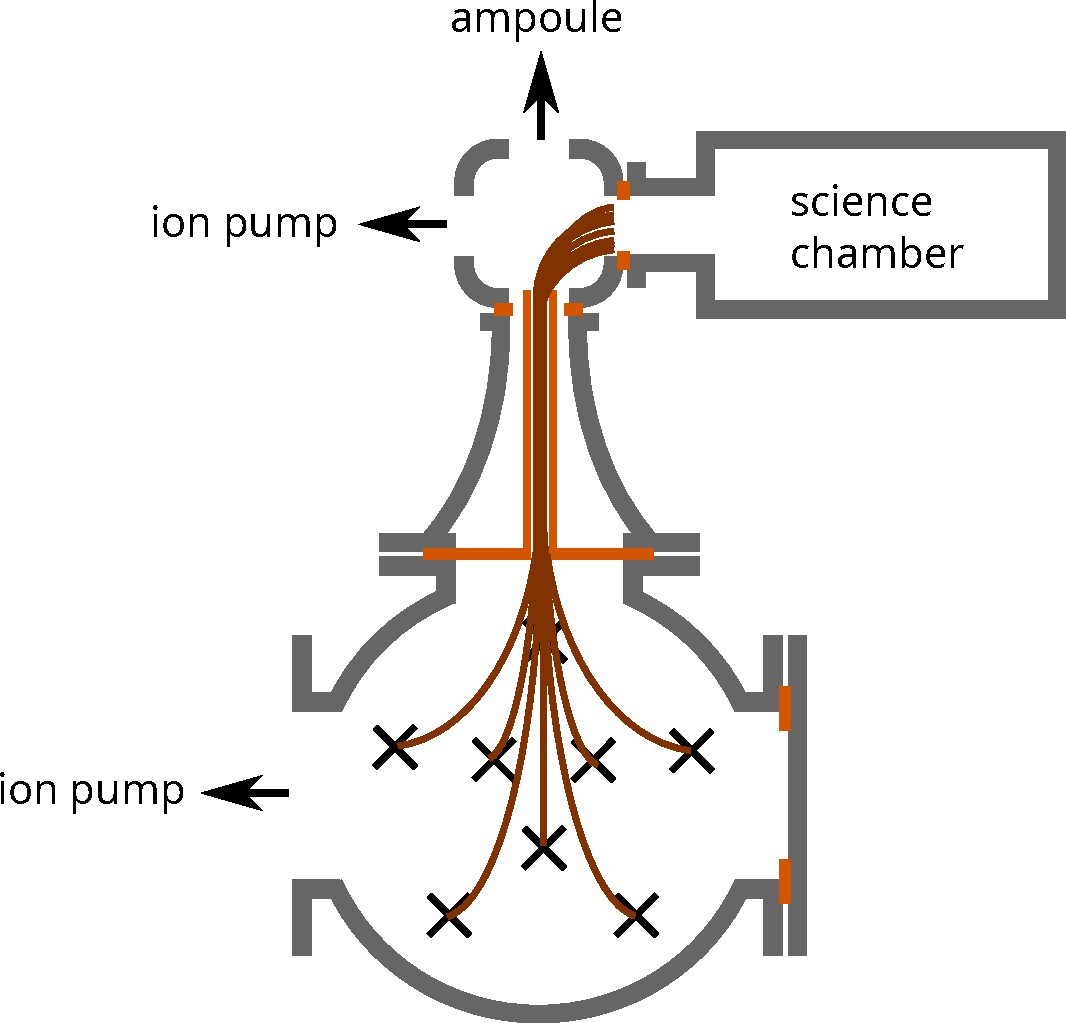
\includegraphics[width=0.5\textwidth]{Images/differential_pumping.pdf}
    \caption{A cross-section illustration showing the copper pinch off tube used as a differential pumping tube between the upper and lower vacuum chamber regions. The 8 fibers coming through the drilled Teflon plugged SwageLock feedthroughs (each feedthrough marked as a black X) go up through the copper tube and into the science region.}
    \label{fig:differential_pumping}
\end{figure}

The vacuum system is divided into two sections, upper and lower, separated by a differential pumping region. This is done in order to shield the science region from small leaks which may be present due to the eight fiber feedthroughs in use. In the section joining the upper and lower chambers, a copper pinch-off tube, cut to a length of 7 cm and with tube inner diameter 6.35 mm, was used in lieu of a standard Conflat copper gasket (see Fig. \ref{fig:differential_pumping}). Additionally, the middle section of the tube was pinched down to approximately a slit of 1 mm width to further reduce the flow conductivity between the two regions. An upper bound for the conductivity of the pipe can be estimated by ignoring the pinch and using the Knudsen flow conductivity in the molecular flow regime (valid for our UHV pressure level),
\begin{equation}
     C = 12.1\frac{d^3}{l}
\end{equation}
for a pipe of diameter $d$ and length $l$, where $l \geq 10d$ \cite{Marquardt1999}. This gives a conductivity of 0.44 L/s between the two chambers, which is lower than the upper ion pump's pumping speed, 10 L/s, by a factor of about 22. The actual conductivity is lower due to the pinch, and the conductivity between the science region and lower chamber is lower still due to the right angle between the science chamber and differential pumping path. In practice, we observed an order of magnitude difference ($P_{\textrm{upper}}=4\cdot10^{-10}$ Torr, compared to $P_{\textrm{lower}}=2\cdot10^{-9}$ Torr) between the two chambers following the vacuum bakeout and prior to opening the valve to release Rb vapor.

\section{UHV science optics}\label{sec:science_optics}

Optics for preparing laser cooling beams, state preparation beams, optical dipole trap, and photon collection are installed in our UHV system. Each beam is prepared by an optical module consisting of a fiber connected to a ferrule installed in a tube containing other optics, including lenses, polarizers, and waveplates, depending on the purpose of the particular module. The components of each module are aligned and glued together using UV-curable UHV-safe epoxy (Optocast 3410 Gen2). The Macor bridge was designed with grooves to pre-align each module, however, some manual alignment of position was required, in addition to alignment of polarization for some of the beams. Active alignment of optics in vacuum, e.g. by piezo control, was foregone in favor of simplifying the apparatus design. In the following sections, the construction of each type of optical module and the subsequent co-alignment of all of the beams is described. 

In the first version of our quantum network node design, the optics in UHV consisted of modules for creating four of six laser cooling beams, two optical pumping/excitation beams, and a simultaneous dipole trap and photon collection path based on a high-NA on-axis parabolic mirror. A complete ``ingredient list" of the parts required to build this version of the network is given in Appendix \ref{ch:ingredients}.

\subsection{Clean room assembly environments}

All of the assembly of the UHV optical components took place inside of two table-top enclosures which mimic a clean room environment. Each enclosure has a HEPA-filtered fan to provide positive pressure from clean air over the optics and tools inside. One of the enclosures or ``clean boxes" was a commercially available solution by Sentry Air Systems (model SS-218-PCR), while the other was custom constructed from transparent acrylic sheets but used the same Sentry Air Systems air purifier (model SS-200-MS). The custom box measured roughly 1 m wide by 0.5 m deep and 0.5 meter tall, about twice the width of the commercial box. Particulate matter levels were tracked in the custom box using a Temtop PMD 331 particle counter, which counts particles of various sizes down to 2.5 $\mu$m. Typical particle counts observed were consistent with a class ISO 4 clean room.

\subsection{MOT and state preparation optics}
Below we discuss the design and construction of optical modules consisting of relatively small bulk optics which set the beam size and polarization of the light for manipulating the atomic states of interest. The assembly of these modules was done mostly by hand with the aid of some custom holders which we 3D printed, a fiber holder (Thorlabs HFF001), and assorted 3-axis translation stages. The procedure is described in what follows. For the first network node, each of these modules was constructed with care by Akbar Safari.

\subsubsection{MOT optics}

The in-vacuum optics for delivering the cooling light, MOT repumper, and excitation repumper consisted of four optical modules which we will refer to as ``MOT tubes" going forward. The MOT tubes are labeled $M1-M4$ in the schematic in Fig. \ref{fig:optical_chip_design}. These four modules create beams in a plane parallel to that of the Macor substrate, whereas the other two MOT beams are delivered by free space optics mounted outside of the chamber. Each MOT tube, with a form factor of $\sim1$ cm$^3$, is used to terminate a PM fiber and replaces the chain of larger bulk optics that would typically be used for creating MOT beams. Specifically, each MOT tube consists of a fiber ferrule, collimating lens ($f=5$ mm, Edmund Optics $\#$48-709), polarizer (Skight Optics, AR coated for 780 nm), and quarter waveplate (Skight Optics, zero-order for 780 nm, AR coated). All of these components are safe for use in UHV. In cases where the manufacturer was unable to guarantee this, we tested components in a small UHV chamber to ensure outgassing (e.g. from optical epoxy or coatings) did not inhibit reaching vacuum at the level of $10^{-10}$ Torr. The optical fibers used (Fibercore HB800P/001), including those used for the other optical modules discussed later in this work, are polyimide coated, which is safe for use in UHV and makes the fiber more resistant to breaking compared to bare fiber. The components for each MOT tube are housed in a 7mm outer diameter glass tube which can be co-aligned to the other optics on the Macor substrate. Each glass tube has two holes drilled in specific locations to allow air to be pumped out from the regions between the polarizer and lens and between lens and the fiber.

For each MOT tube, a PM fiber of approximately 2 m in length was used, where one end was connectorized with an APC connector and the other end was cleaved. We initially used a bare fiber adapter to couple into the fiber, but found this to be mechanically unstable. The connector facilitated more stable coupling of light into the fiber during the alignment procedure. The cleaved end of the fiber was inserted and glued into a fiber ferrule which in turn was inserted and glued into a Macor sleeve, which held the 1.8 mm diameter ferrule in the 5 mm bore of the glass tube housing the optics. The surface of cleaved end of the fiber was checked for damage before and after inserting into the ferrule with the aid of an inexpensive microscope (Carson MP-250). Both the ferrule assembly and collimating lens were inserted in the glass tube, first without glue, to check the quality of the collimated beam in both the near and far field (about 80 cm from the lens). This step was followed by cleaning the lens with a lint-free q-tip and acetone/methanol solution as needed, until the beam shape was deemed acceptable. After this the ferrule assembly were removed then reinserted with glue and realigned for checking the beam a final time before curing the glue. 

The polarizer used on a MOT tube was aligned to the slow axis of the fiber in order to mitigate amplitude fluctuations on the light after of the MOT tube. Because the key of the APC connector on the fiber was installed at an initially unknown angle with respect to the slow axis of the fiber, it was necessary to couple the light into the fiber in free space and then tune the polarization state into the fiber with waveplates. This procedure was done using a polarimeter (Thorlabs PAX1000IR1) to check that the polarization state of the light after the MOT tube was linear with minimal variation when the stress was applied to the fiber by hand. Coupling to the slow axis was distinguished from coupling to the fast axis by first measuring the approximate angle between the slow axis and key of the APC connector with a microscope, and then making sure the angle of the linear polarization as measured by the polarimeter matched this. After this step, the polarizer was glued in place after rotating it by hand to maximize the transmitted power and checking the transmitted beam quality. Finally, a quarter waveplate was inserted into the end of the tube and aligned while monitoring the polarimeter to set the polarization state of the light to be left-hand circular (optics handedness convention).

\subsubsection{State preparation optics}

After cooling and trapping a single atom in a dipole trap, the atom needs to be optically pumped into a particular internal electronic state before attempting to create atom-photon entanglement. After this optical pumping (OP) phase, the atom will be excited in order to let it decay to the desired target states for entanglement preparation. The light for both the OP and excitation can be coupled into either one or both of two shared fibers which are terminated with optical tubes oriented perpendicularly to the dipole trap (parabolic mirror) axis, one on each side. These optical modules consist of a fiber ferrule, graded-index (GRIN) lens (EFL=), and a polarizer (Skight optics), housed in a 2.8 mm diameter glass tube. We will refer these modules as GRIN tubes 1 and 2, labeled as $G1$ and $G2$, respectively, in Fig. \ref{fig:network_node_apparatus_schematic}.

As with the MOT tubes, PM fibers with roughly 2 m length were first prepared, cleaved on one end and connectorized and polished on the other, with the cleaved ends inserted and glued into glass fiber ferrules. For these modules, the cleaved fiber tips were inserted far enough to stick out of the fiber ferrules, then retracted until even with the end of the ferrule. This is because the GRIN lenses used were design to give a collimated output beam when butted up against the fiber. The ferrule and GRIN lens were inserted into the glass tube one at a time and glued. As with the MOT tube housings, the glass tubes for the GRIN assemblies also have holes drilled to facilitate pumping out the residual air between the optics.  Finally, a polarizer was aligned and glued on the tube in the same fashion as described in the previous section. 

Notably, the beam quality out of the GRIN lenses was substantially worse than that of the beam out of the spherical plano-convex lenses used in the MOT tubes. The reason for this is not known, and the GRIN lenses did not have any aberrations visual to the eye when viewed at an angle under the Carson microscope. The comparison in beam quality is shown in Fig. \ref{fig:assembled_optical_tubes}.

\begin{figure}[ht]
    \centering
    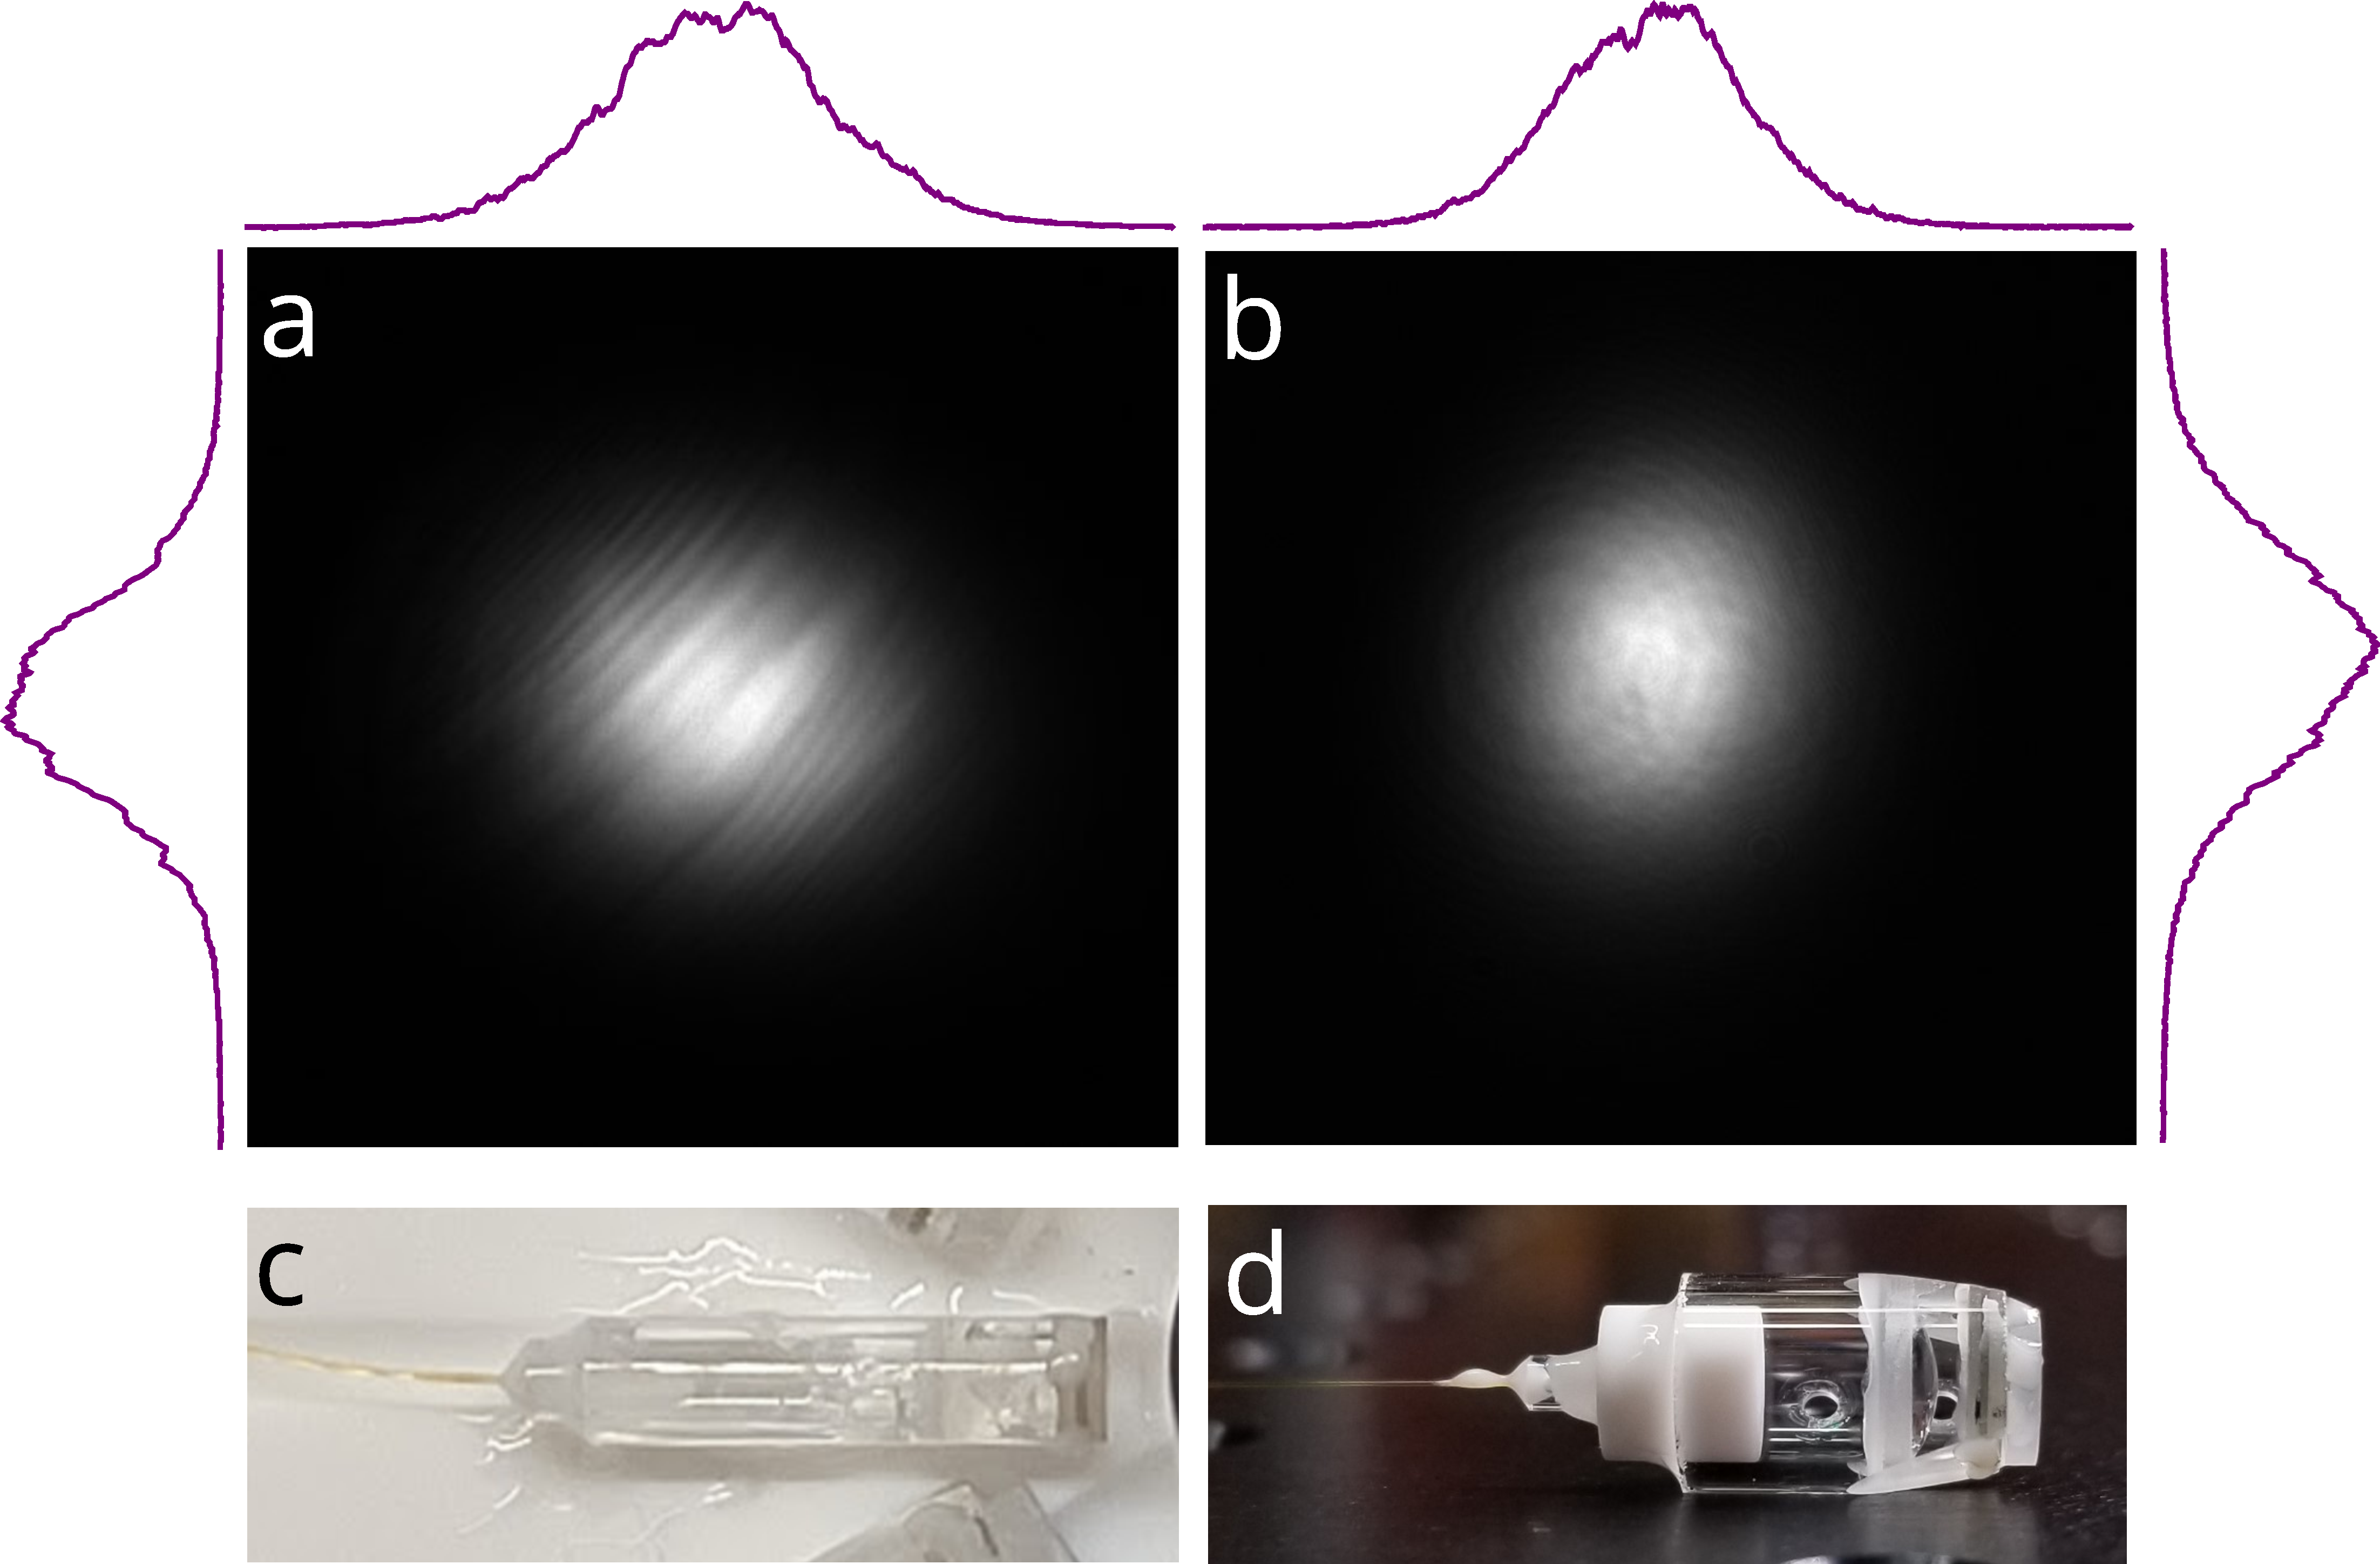
\includegraphics[width=0.8\textwidth]{Images/MOT_and_GRIN_tubes.pdf}
    \caption{Photos of assembled optical modules and their resulting beam profiles. The beam profiles shown are from \textbf{a} GRIN 2 and \textbf{b} MOT 1. The purple curves are cross sections of the beams. A typical MOT and GRIN tube are shown in \textbf{c} and \textbf{d} respectively. Although the quality of the beam produced by the GRIN lens is much worse than that produced by a standard glass lens of uniform refractive index, because the atom will be confined to an area of order $1 \mu$m$^2$, this aberrated beam profile is expected to be inconsequential.}
    \label{fig:assembled_optical_tubes}
\end{figure}

\subsection{Parabolic mirror: dipole trap and photon collection}\label{sec:mirror}

\subsubsection{Mirror optics design}

In the first version of our quantum node design, photon collection and dipole trap were implemented with the same optical path, composed of an SM fiber (FiberCore SM800(4.9/125)P/001), an achromatic doublet (Edmund $\#$47-377), and a custom high-NA on-axis parabolic mirror (NiPro Optics). The fiber ferrule was mounted in a Macor ring, which in turn mounted into a machined Macor tube along with the lens and the mirror. The fiber was chosen to be SM, which affords the greatest flexibility, because the target photon emission from the atom will be $\sigma$ polarized, while the dipole trap light will be $\pi-$polarized. 

A parabolic mirror was chosen over refractive high-NA optics since reflective optics are inherently achromatic, allowing us to align the optics for both photon collection at 780 nm and a dipole trap near 852 nm simultaneously. The entire photon collection optical train is then nearly perfectly achromatic, as the doublet lens has much less than 1 $\mu$m axial chromatic shift between 780 nm and 852 nm light, as checked with Zemax OpticStudio. The custom mirror, manufactured by NiPro optics, is made of diamond-turned 6061 aluminum body coated with a protected silver coating. For dimensions of the mirror, see the mechanical drawing given in \ref{ch:mech_drawings}. The mirror was baked in air by NiPro up to 130 $^{\circ}$C, ramped at 2 deg/min, and held at this temp for 16 hours before ramping down, to ensure that the coating would not peal off at this temperature. The mirror was designed to have a working distance of 5.26 mm and clear aperture NA of 0.61, corresponding to over 14$\%$ collection efficiency, given by,
\begin{equation}
    \eta = 2\pi\int_{0}^{\sin^{-1}(\text{NA})} E_{\sigma_{\pm}}(\theta)^{\ast} \cdot E_{\sigma_{\pm}}(\theta) d\theta 
\end{equation}

for $\sigma$ light if the quantization axis is taken to be along the axis of the mirror. $E_{\sigma_{\pm}}$ is the probability density function for circularly polarized emission from a radiating dipole as pattern as a function of emission angle. This collection efficiency does not, however, tell how much of the light can be coupled back into a single mode fiber. The finite aperture of the mirror is comparable to the diameter of the ideal Gaussian mode for mode matching to the SM fiber. The mirror also has a central through hole, explained below. To estimate the collection efficiency into a single mode fiber, the system was modeled in Zemax OpticStudio, with the atom approximated as a point source emitting rays isotropically into the solid angle spanned by the mirror. This calculation predicts a coupling efficiency of $78\%$ into the SM fiber.

The mirror has an on-axis through-hole of 0.5 mm diameter to allow collimated dipole trap light to pass through. This allows for tuning the degree of linear polarization of the dipole trap by maximizing the light transmitted through a linear polarizer placed behind the mirror and coupled out of the vacuum system with an optical fiber. An optical module was constructed for this purpose, which is the same as one of the MOT tubes except that it lacks a quarter waveplate, and is terminated with a multi-mode fiber (Thorlabs UM22-200) to maximize the amount of light coupled out of the system. In the experiment, we can monitor and maximize the dipole trap light coupled into the MM fiber, using waveplates before the SM fiber which sends the light to the mirror. This allows us to tune the dipole trap to be linear, though we note that this only provides a starting point for tuning the polarization. For a tightly focused dipole trap, the collimated input light should be slightly elliptical to minimize heating in the trap \cite{Garcia2018}. 

\subsubsection{Alignment and characterization}

Aligning an on-axis mirror presents a significant challenge, as the focal spot cannot easily be viewed directly without obstructing the beam incident on the mirror. Additionally, because of the high NA of the mirror, tilt of as much as 0.05 degree can introduce significant coma, as checked in Zemax OpticStudio. In order to aid in alignment, the tolerance between the mirror and Macor tube was specified at less than 40 $\mu$m (a compromise to allow for the larger thermal expansion of the aluminum compared to Macor) and the mirror body was made to be 12 mm long, 10 mm of which sit in the Macor tube. This essentially guarantees that the mirror body is well-oriented to the tube axis. 

A tapered fiber can be used as an approximate point detector, by coupling light into the fiber tip and measuring the output at several coordinate points in space to directly measure the shape of an optical intensity pattern \cite{TOLEDOCROW1995,RHODES1998}. In this way, we were able to directly map the focal intensity pattern produced by the mirror. The width of the cladding on the tapered fiber used (K-Tek Nanotechnology E50-780HP, uncoated tip) was only 125 $\mu$m, such that the length of fiber extending in front of the mirror, equal to the radius of the mirror or 4.1 mm, does not obscure a significant fraction of the light incident on the mirror. The fiber tip was held and moved using a piezo stage (Thorlabs NanoMax 603D) controlled by a LabVIEW program to take 2D raster scans of the field and record the signal out of the fiber with a photodetector (Thorlabs APD430A) at each positional step. 

To align the mirror, doublet, and fiber, the fiber-ferrule assembly and doublet were inserted into the Macor tube and adjusted to give a collimated beam at 780 as verified with a shearing interferometer. The fiber and lens were both held with custom 3D printed fixtures held by a 3-axis translation stage with 2-axis tilt and 2-axis rotation stage, respectively. The fiber assembly was tilted to steer the beam to propagate roughly along the axis of the mirror tube. The mirror was then inserted into the Macor tube and glued in place. The fiber tip was moved into the approximate location of the focal field by eye, sometimes by observing the scattering of 780 nm light off the end of the fiber. About 15 mW of light on the mirror, and the observed coupling efficiency into the fiber tip was on the order of $10^{-5}\%$. The remainder of the alignment was done by iteratively making an adjustment to the tilt of either the fiber or doublet, and running the raster scan code to see the current shape of the focal intensity pattern.

\begin{figure}
    \centering
    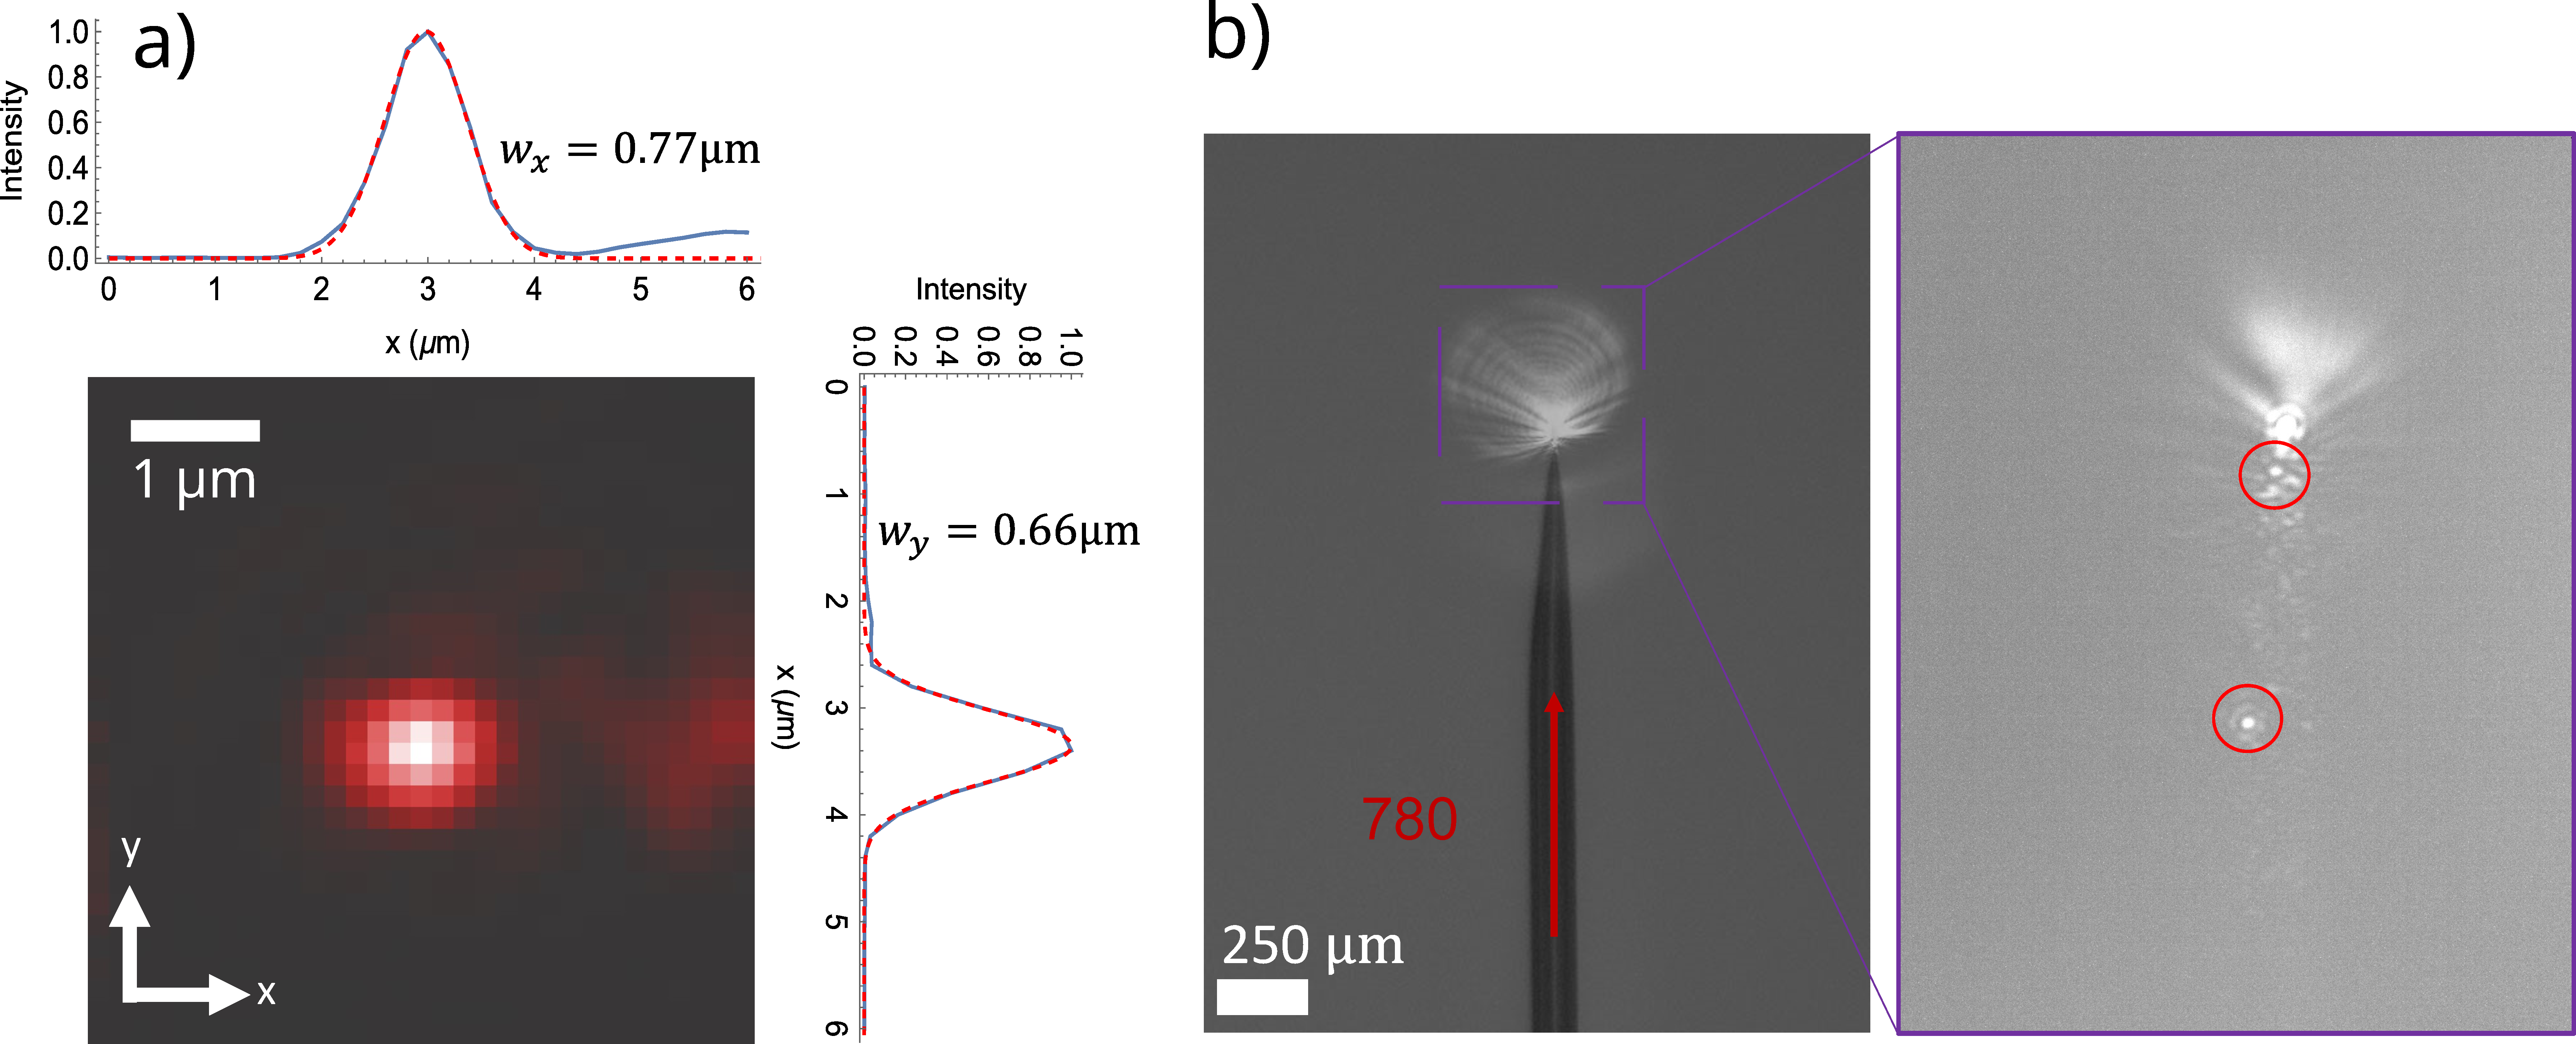
\includegraphics[width=\textwidth]{Images/mirror_focus_fiber_scan.pdf}
    \caption{\textbf{a)} The mirror focal intensity pattern as measured by coupling light from the mirror into a tapered fiber tip with a raster scan. Gaussian fits are shown for slices in $x$ and $y$, where the fiber tip pointed along $-y$. The step size of the scan was 200 nm in each direction. The apparent aberrations on the beam are due to coupling into defects in the fiber tip, shown in \textbf{b)}. By coupling light into the non-tip end of the fiber, we can see that the emission, and hence collection, mode shape is not truly point like. The left and right images show the fiber with lower and higher exposure and zoom, respectively, to make clear the structure of the tip mode (left) and the weaker defect modes (right).}
    \label{fig:mirror_fiber_scan_post_gluing}
\end{figure}

The image of the focal intensity pattern, after optimizing the alignment and gluing the fiber assembly and doublet, is shown in Fig. \ref{fig:mirror_fiber_scan_post_gluing}. The fitted $1/e^2$ Gaussian waists are $w_x=0.77~\mu$m and $w_y = 0.66~\mu$m, where x and y are the along the fiber axis and perpendicular to the fiber, respectively. These values are within about $20\%$ of the diffraction limited value given by $\lambda/(2 NA)$. Note that the beam exhibits apparent aberration along direction x but only on one side of the beam. This is an artifact of weak coupling of light into defects in the stem of the fiber tip, which are shown in Fig.  \ref{fig:mirror_fiber_scan_post_gluing}b and was verified by rotating the mirror tube 90 degrees with respect to the fiber tip and repeating the scan, which shows that the aberrations show up in the same place with respect to the fiber tip. This second scan showed the aberrations in the same place with respect to the fiber, confirming they were not from the intensity pattern.

A full reconstruction of the three-dimensional shape of the beam focused by the mirror can be done using the tapered fiber. To approximate this, several transverse scans of the beam were taken, with 0.5 $\mu$m longitudinal (i.e. along the mirror axis) steps between each slice. The result is shown in Fig. \ref{fig:fiber_scan_axial_steps}, where it can be seen that the beam appears to distort and translate as it expands. This can be mostly explained by coupling of the light into the tapered fiber defects as well as a slight angle between the true axis of the beam propagation and the axis of the fiber longitudinal steps. 

\begin{figure}
    \centering
    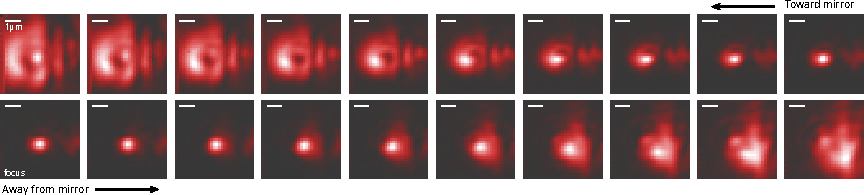
\includegraphics[width=\textwidth]{Images/fiber_scan_tranverse_slices.pdf}
    \caption{Transverse slices of the dipole trap beam taken at several axial positions about the focus. Each pixel is 200 nm and the longitudinal position varies by 0.5 $\mu$m between each slice. Note that each slice has been individually normalized for clarity.}
    \label{fig:fiber_scan_axial_steps}
\end{figure}

Additional fiber scans were done using 852 nm light to illuminate the mirror, in order to verify the expected low chromatic shift between the emitted photon light at 780 nm and the dipole trap light. However, it was observed that the tapered fiber position drifted monotonically on the order of 100 nm over a minute while we were making some of the measurements, such that subsequent raster scans in the same space showed an apparent drift the peak focal intensity. In order to characterize the difference in the positions of the focus at 780 nm and 852 nm even in the midst of this drift, we took a series of scans alternating between the two wavelengths at each scan. Because the drift was primarily along one axis of the available scan degrees of freedom, we were able to scan such that the drift would be confined in that the plane and we could repeat the scans without changing alignment between them. The results of this series of measurements is shown in Fig. \ref{fig:780_852_fiber_scan}. By fitting the drift of the focus along $z$ at each wavelength individually, we find an average difference of 72 nm between the $z$ positions of the focus at the two wavelengths over the hour scan time. In the other transverse direction, $y$, we infer a difference $<$ 200 nm, which is the resolution of the scan in this direction. Finally, we infer an axial chromatic shift of $<$ 500 nm.  

\begin{figure}
    \centering
    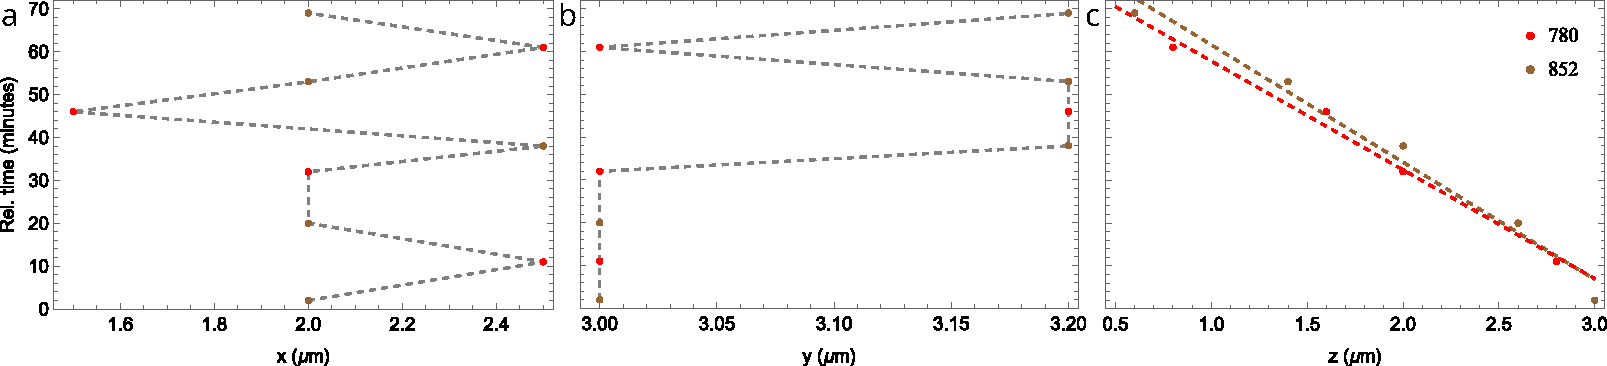
\includegraphics[width=\textwidth]{Images/fiberscan_852_780_xyz_fig.pdf}
    \caption{Tapered fiber scan measurement of chromatic shift between 852 and 780 nm light focused by the parabolic mirror. \textbf{a}, \textbf{b}, and \textbf{c} show the coordinate of the brightest pixel for a given 3D scan at either 780 (red points) or 852 (brown points), at $x$,$y$, and $z$, respectively. In the lab frame, gravity points along $-\hat{z}$, the fiber tip points along $\hat{y}$, and the detected beam propagates along $\hat{x}$. In each 3D scan, the step size is 200 nm in $y$ and $z$ (i.e. in the transverse planes), and 500 nm in the axial direction. The dashed lines in \textbf{a} and \textbf{b} are guides to eye, whereas the dashed lines in \textbf{c} are linear fits to the data for each wavelength.}
    \label{fig:780_852_fiber_scan}
\end{figure}

\subsection{Co-alignment of the on-chip optics}

Once the optical modules had been assembled, they were aligned one at a time on the Macor chip. The location of a trapped atom in experiments will be within the focus of the parabolic mirror, which is a volume of order 1 $\mu$m$^3$ All of the other beams, which have comparatively much larger cross-sections, need to overlap the focal region of the parabolic mirror. Additionally, the pairs of counter-propagating MOT and excitation beams should have their k-vectors roughly anti-parallel. The polarization degree of freedom of the optical pumping beams also needs to be aligned with respect to the optical axis of the dipole trap. Because each additional optical model added to the chip introduces an additional blind spot, the order of operations to co-align the beams is critical. 

During the alignment process, a method was needed to view the focused spot of the mirror as well as the other, much larger beams, without significantly blocking light incident on the mirror. A thin flat semi-transparent sheet with negligible cross section compared to the area of the mirror could be used as a scattering surface, as shown schematically in Fig. \ref{fig:scattering_sheet_method}. We made a makeshift thin diffuser surface by rinsing a strip cut from a transparency sheet with acetone and subsequently blowing it dry with canned air, which created a uniform cloudy finish on one side. The sheet had a thickness of 80 $\mu$m and could be inserted through the central hole in the Macor bridge with the plane of the sheet coincident with the mirror tube’s optical axis. The rough positioning of the sheet, with the help of a 3-axis translation stage, was done by eye and with a camera looking down on the bridge from above. The stage also allowed for retracting the strip back down through the bridge to allow the beams to pass unobstructed as is necessary at various stages of the alignment.

\begin{figure}[t!]
    \centering
    
\includegraphics[width=\textwidth]{Images/beam_projection_imaging_schematic.pdf}
    \caption{Schematic of the setup to image the optical chip beams as projected on a transparent scattering sheet made from an acetone-rinsed transparency sheet.b  \textbf{a} Cross-section of the optical chip from the side showing the transparency sheet in the path of the beam incident on and reflected by the mirror, and the projection of a MOT beam (light red oval). \textbf{b} View of the optical chip and transparency sheet from the top, showing the imaging path. \textbf{c} A photo of the optical chip showing the transparency sheet. Inset \textbf{d} shows the transparency sheet which appears matte white after the acetone rinse, and inset \textbf{e} shows its surface under an inexpensive microscope, captured with the author's phone's camera. The apparent bulge is due to optical aberration.}
    \label{fig:scattering_sheet_method}
\end{figure}

It is worth noting a couple of technical points that constrained the way in which we aligned the optics. The machining tolerances between the cylindrical grooves on the Macor bridge and the tubes housing the optical components were of order 10 $\mu$m, which ensures that the optical modules should be close to the correct alignment for ``free” as soon as they are placed on bridge, with the exception of the parabolic mirror tube for which the axial degree of freedom must be adjusted. However, imperfection in either the placement of fibers and lenses in the tubes or imperfections in the lenses in themselves result in the beams traveling off axis or at slight angles to the axis of the of the machined grooves on the bridges, and these errors can only be corrected provided they are small. In particular, rotating the MOT beam tubes about their axis in the grooves allowed us to walk the beam position at the center of the bridge, typically by as much as 100 $\mu$m, but transverse positioning of the optical modules was extremely limited due to the close tolerances. 

To begin the alignment, both pairs of MOT tubes were placed on the bridge to check whether we could observe coupling of light output by one MOT tube into the fiber of the module opposite of it. One MOT tube was held in place with a 3D printed clamp using neodymium magnets above and below the Macor bridge, while the opposite MOT tube was rotated about its axis and poked by hand while the signal of a photodetector (TTI TIA-525) connected to the output fiber was observed on an oscilloscope. If no coupling was observed by moving only the unclamped MOT tube, the other was adjusted incrementally. Once coupling was observed with both pairs of MOT beams, it was verified that the beams were roughly aligned using a piece of matte Scotch tape as a scattering screen placed at the intersection of two beam coming one side of the parabolic mirror axis. None of the MOT tubes were glued in this preliminary check. Going forward, we will refer to the MOT tubes by numbers 1 through 4, as shown in Fig. \ref{fig:optical_chip_design}.

The science region, defined by the location of the mirror focus, was set by the intersection of MOT 1 and the mirror focus by axial adjustment of the parabolic mirror tube while viewing the overlap of the two beams on the transparency strip, as imaged through the side of the mirror tube with a zoom lens and CCD camera (ThorCam CS165MU1). MOT 1 was glued in place, in the position that it was left in after observing coupling to MOT 3 in the preliminary step, since it was not guaranteed that positioning the beam of MOT 1 to be exactly centered on the mirror would allow for coupling to MOT 3, which guarantees sufficient alignment of this MOT beam pair. For gluing of MOT 1, the mirror tube, and all other components below, the epoxy was applied in a small amount with a thin piece of solder used an applicator such that the applicator would be more likely to bend than to misalign the optical being glued if too much force was applied. UV light (UV wand model?) was applied for at least 60 s to each glued region.

Next, GRIN 2, situated on the same side of the mirror tube as MOT 1, was aligned. For this beam, the polarization alignment mattered as well as the position, such that free rotation of the optical tube to walk the beam to the best position was not possible. Due to space constraints on the bridge and the small diameter of the GRIN tube, it was not feasible to grab it with some kind of clamp while retaining sufficient freedom to move it. Instead, a 4 mm Thorlabs cage system rod was glued to the top of GRIN 2 after first roughly aligning the polarization. This rod, held by a 6-axis stage (3 translational d.o.f., 3 rotation), could then be used to precisely align both the position and polarization of the GRIN tube before gluing the tube in place and then gently breaking the rod free from the GRIN tube. This last step was confirmed to work in advance with a spare GRIN tube, rod, and Macor bridge to ensure the glue joint between the Macor and glass would win over the glass to steel joint. The 6-axis stage was constructed from off-the-shelf optomechanics.

The alignment of the polarization of the optical pumping beams produced by the GRIN tubes, relative to the photon collection axis, is critical. In many cold atom experiments, the optical pumping fidelity can be optimized by tuning both the polarization of the light and modifying the angle of the quantization axis with the magnetic shim fields. However, the fidelity of the atom-photon superposition states we generate depends on our ability to collect only $\sigma$-polarized light into the optical fiber. That is, changing the angle of the magnetic bias field to optimize optical pumping fidelity to compensate for polarization misalignment will in general come at the cost of collecting unwanted $\pi$-polarized photons which lower the entangled state fidelity. 

To align the polarization of the GRIN tubes, we first assume that the photon collection axis lies in a plane parallel to the plane of the bridge, and use a PBS (Foctec 780 nm High Extinction PBS) sitting on the bridge to define the target polarization axis. The GRIN 2 beam was roughly aligned to transmit through the PBS, corresponding to polarization lying in the plane of the bridge, then glued to the 4mm cage rod. The transmission of the light through the PBS is insensitive to small changes in the polarization angle, so we employ a slope detection method for fine tuning. 

A slope detector was made consisting of  motorized rotation stage (Thorlabs K10CR1) holding a linear polarizer (Thorlabs LPNIR100), followed by a photodetector whose output went to an analog input device (NI 782602-01) which could be read by a LabVIEW program which also controlled the rotator. By rotating the polarizer $\pm 45^{\circ}$ about a central $\theta_0$ and taking the difference of the transmitted intensity at those endpoints, we can programmatically feedback to the position of $\theta_0$ to align the polarizer to the reference polarization, i.e. that of the light passing through the PBS. The error in this process, accounting for the uncertainty and repeatability of the K10CR1, is $\sim 0.02^{\circ}$. After $\theta_0$ has been set to within this uncertainty, the same method of slope detection can be used to align the GRIN beam polarization with the PBS removed from the bridge. In this step, the polarization is manually adjusted in between the polarization measurements. The angular error, when it is small, can be estimated from the intensity difference at $\pm 45^{\circ}$ as $\delta \theta = -2(I(45^{\circ}) - I(-45^{\circ}))$. 

After aligning the polarization of GRIN 2 using the above method, the position was tuned to overlap the parabolic mirror focus on the transparency strip as best as possible within the mechanical constraints of the bridge. The final polarization error was measured to be $0.05^{\circ}$ after gluing.

For GRIN 1, we were not able to directly measure the polarization of the beam, since it gets blocked by GRIN 2. Instead, we aligned a polarizer on the bridge near where the end of GRIN 1 will go, using the method described above with the beam output by GRIN 2 as the reference polarization. The polarizer was roughly aligned to maximally transmit the GRIN 2 beam, then placed in a small amount of uncured glue on the bridge and poked into alignment with a tweezer by hand until the error could not be further reduced. The final error measured after gluing was $0.2^{\circ}$. 

To install GRIN 1, the ThorCam was pointed anti-parallel to the MOT 1 beam axis, from the MOT 3 side. Using the transparency sheet method, GRIN 1 was aligned to maximizing both the overlap with the parabolic mirror focus and the amount of light transmitted through the polarizer glued in the last step, since GRIN 1 has a polarizer glued to its output.

Projections of the images of the individual beams on the transparency sheet, made by summing the rows and summing the columns, show the extent to which the beams are co-aligned. This analysis is shown for three combinations of beams in Fig. \ref{fig:final_beam_projections}, including all beams except MOT 3, which blocked the imaging path once installed. MOT 3 was installed and aligned by coupling light from MOT 1. It is clear that the parabolic mirror focus is closer to the plane of the bridge than the centroids of the other beams. Nevertheless, because the other beams are much larger than the mirror focus we did not anticipate this being an issue. 

\begin{figure}[t!]
    \centering
    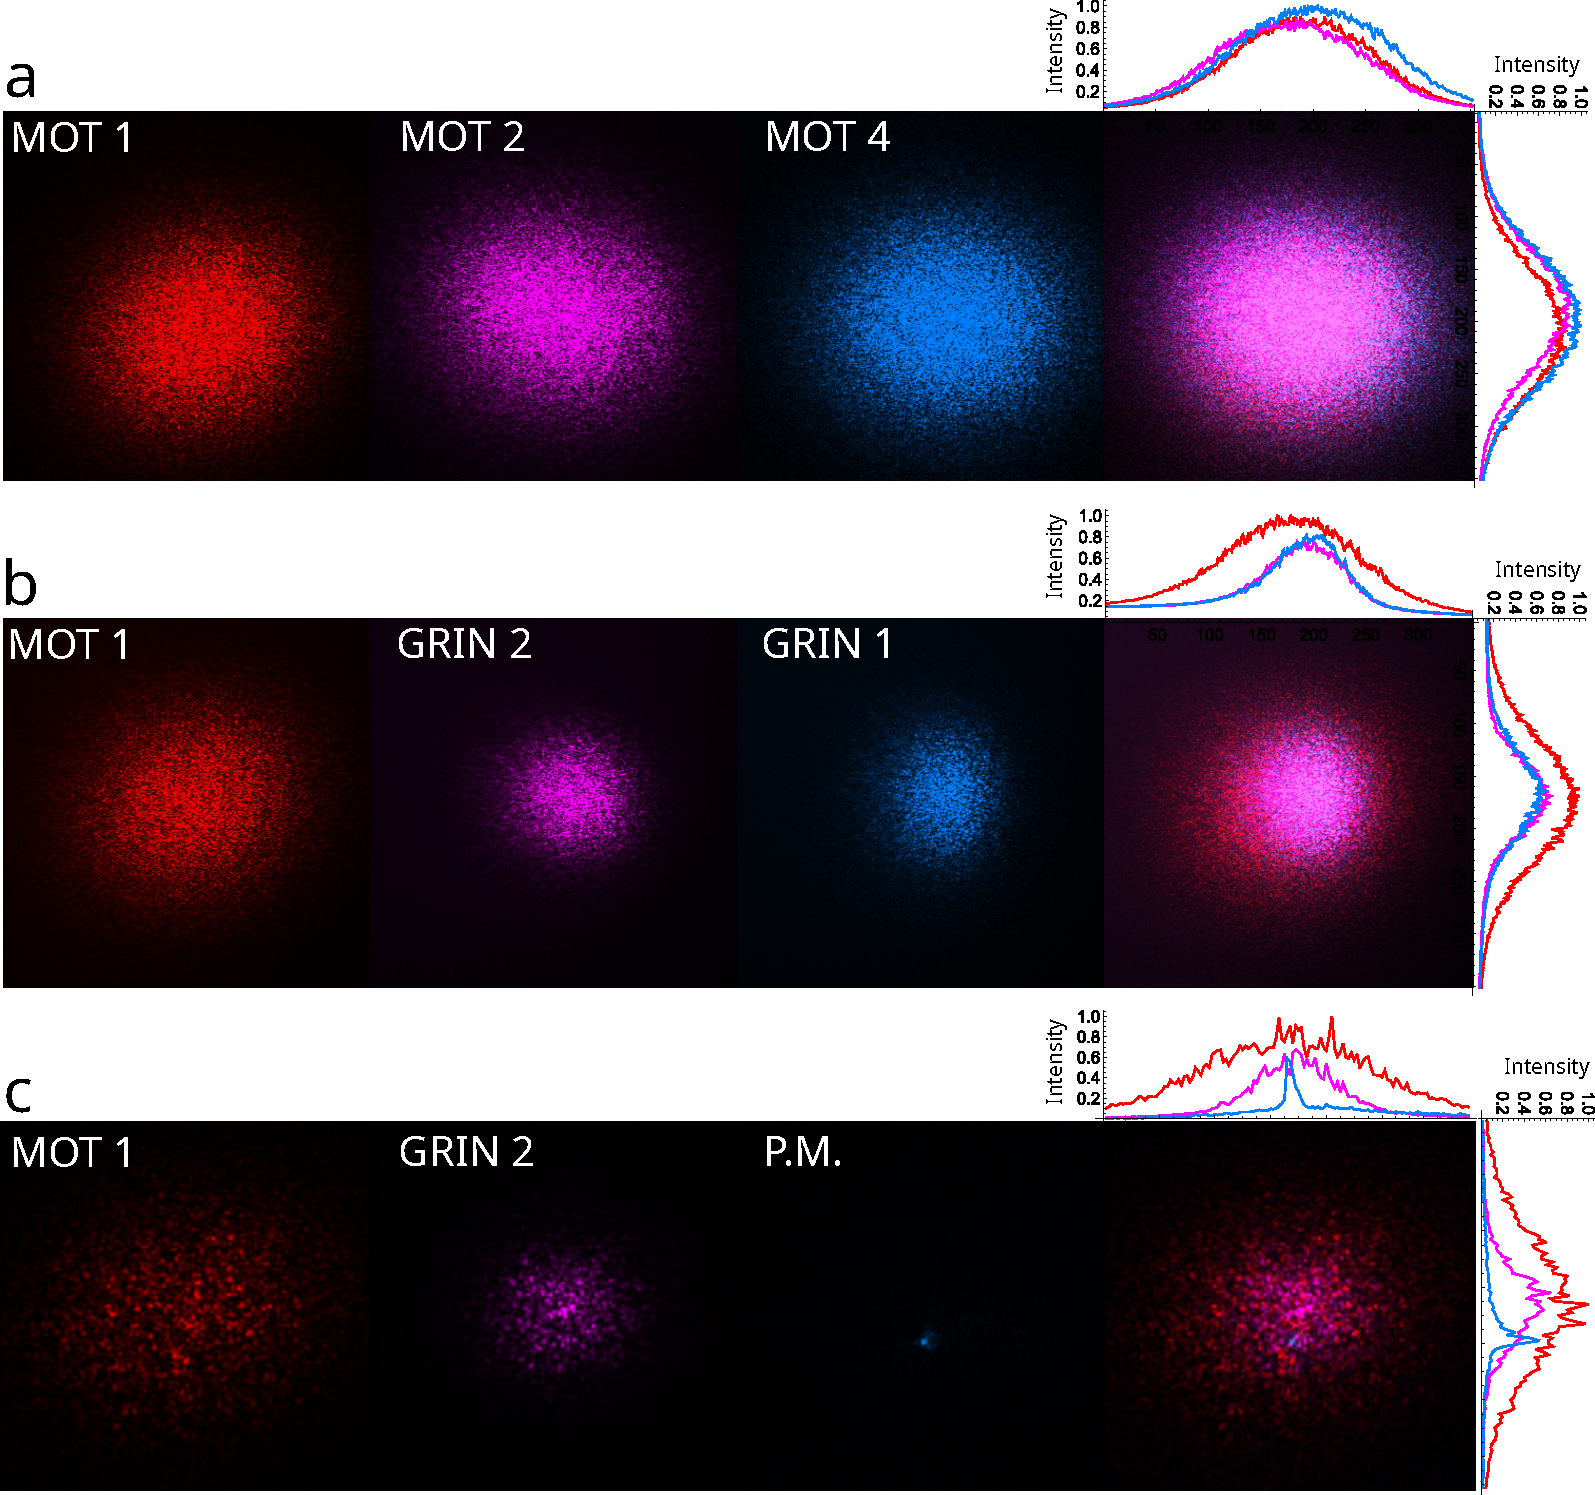
\includegraphics[width=\textwidth]{Images/transparency_sheet_beam_projections.pdf}
    \caption{Optical chip beam projections on an acetone-rinsed transparency sheet. A setup of the imaging schematic is given in Fig. \ref{fig:scattering_sheet_method}. The three panels \textbf{a}-\textbf{c} show different combinations of beam images, where the right-most image in each row is a combined image from the three individual beam images. The curves on the top and right sides are the sums of the rows and columns, respectively, for the individual beams. The ``P.M." image in \textbf{c} shows the focus of the parabolic mirror.}
    \label{fig:final_beam_projections}
\end{figure}

Lastly, an optical module for optimization of the degree of linear polarization of the dipole trap light was installed behind the parabolic mirror. Slope detection was not possible for this configuration. Instead, the same PBS used earlier was placed on the bridge behind the mirror and the polarization state of light coupled into the parabolic mirror SM fiber was tuned with free space waveplates to maximize the light transmitted through the PBS, corresponding to vertical polarization with respect to the bridge. The PBS ports were monitored to verify that the polarization state was not changing over several hours. Then the polarization module was aligned on the bridge by rotating about its own axis to maximize the light coupled out of the MM fiber before gluing this final module in place.

Finally, we note a couple of unexpected barriers that were encountered during the assembly described above. First, some excess cured epoxy on the parabolic mirror tube near the doublet lens prevented it from sitting correctly on the bridge. To remedy this, we removed some material from the bridge using a Dremel with a standard grinding attachment. Second, the epoxy used for gluing the last few optical modules to the bridge, which must be kept frozen when not in use, seems to have expired prior to the date. This was probably due to its being shipped without insulation or dry ice, as had been done with an earlier shipment we received. We realized that the epoxy was expired by noting that UV was not turning the glue completely hard to the touch. However, in the interest of not waiting a few more months for new glue, we modified our glue curing procedure. Following the standard minute-long exposure to UV, which partially hardened the glue, we applied a heat gun with a directed flow at 150 $^{\circ}$C to the glued area. 

\subsection{Optical chip installation and vacuum bakeout}
Following the gluing of the optical modules, the bridge was installed in the chamber and some final diagnostics were performed prior to completing the vacuum system. Installing the optical chip inside the science chamber was a formidable challenge of its own, largely because of the fragility of the fibers. In particular, near the glue joints fixing the fibers to their ferrules, it is easy to snap a fiber, rendering the optical module unusable and irreparable. This happened once while installing one of the GRIN tubes, and other times during the construction of the optical modules. To reduce the possibility of breaking fibers while installing the optical chip in the chamber, the fibers were strain-relieved to the Macor bridge with additional epoxy, after first bending the fibers to fit within the chamber. This step was done with the use of a bendable 3D-printed guide to mimic the perimeter of the inner wall of the chamber, which was safer than working with the chamber itself. We note that the bending radius for the fibers used is about 1 cm, and the optical chip layout was designed to satisfy this, albeit marginally. 

\begin{figure}[h!]
    \centering
    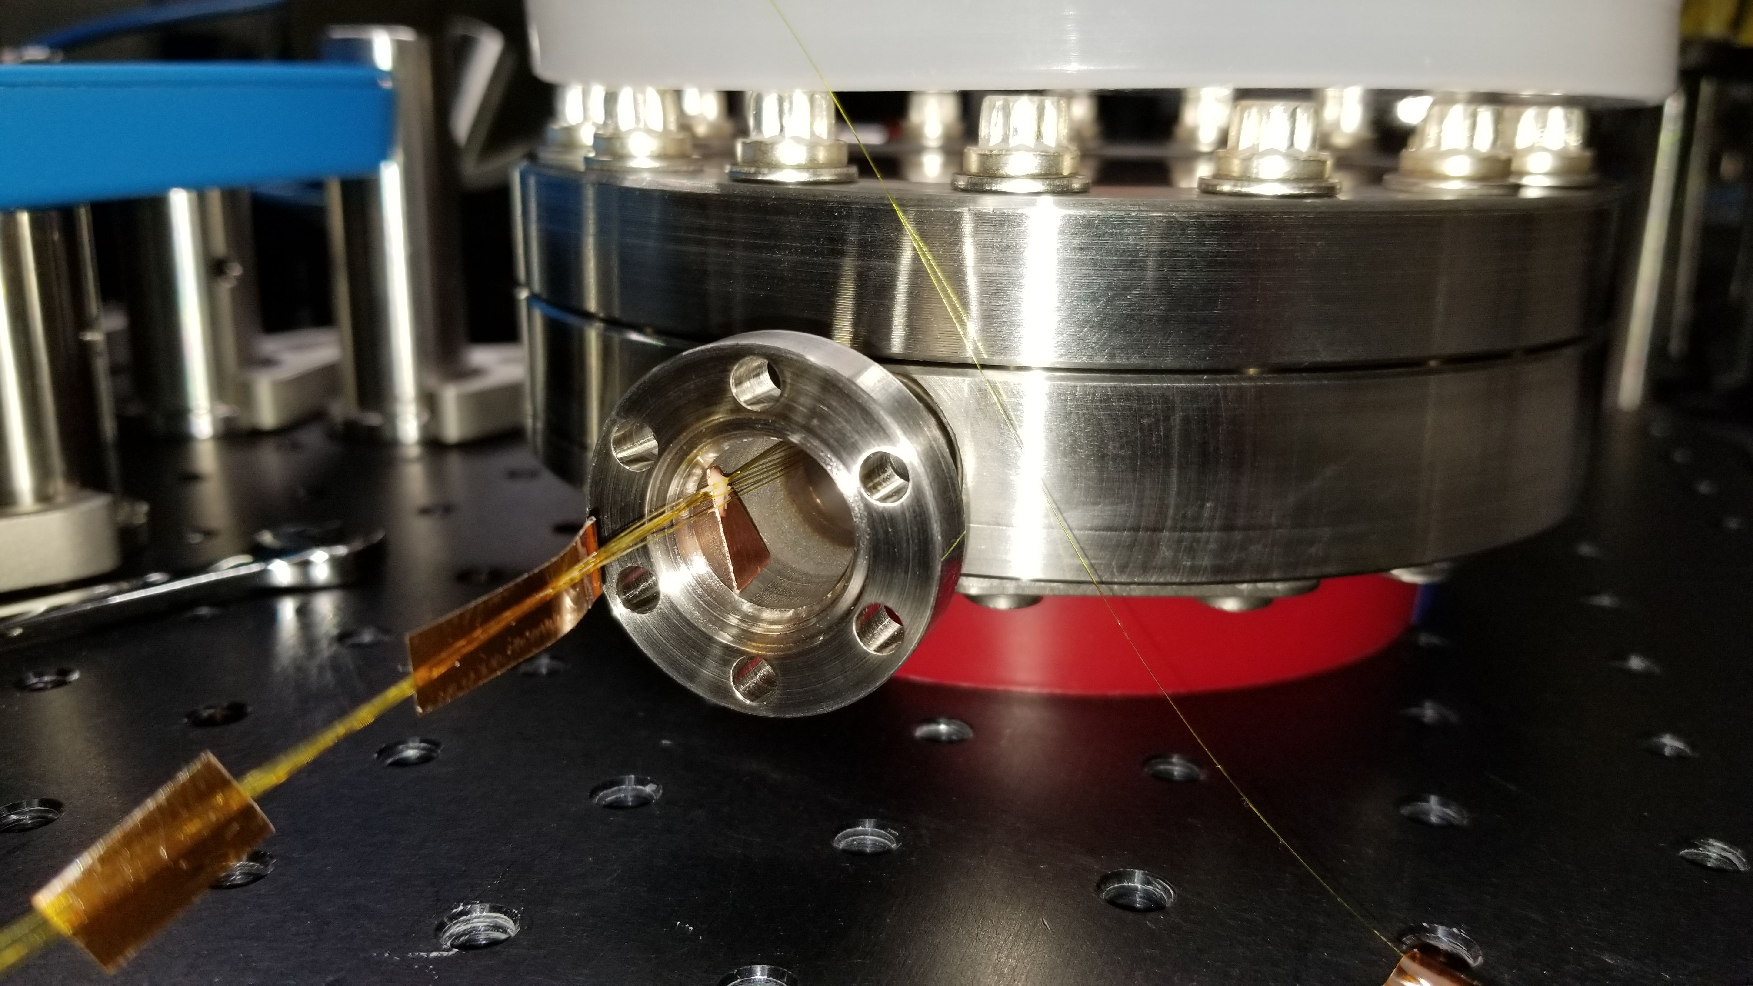
\includegraphics[width=0.7\textwidth]{Images/chamber_fiber_strain_relief.pdf}
    \caption{The optical fibers passing through the neck of the chamber were strain relieved by gluing a piece of the copper sheet to the chamber neck and gluing the fibers in turn to the copper. Note also the pieces of Kapton which can be seen securing the fiber bundle which is emerging from the chamber neck.}
    \label{fig:chamber_neck_strain_relief.pdf}
\end{figure}

To install the optical chip in the lower half of the science chamber, the fibers were fed through the neck of the chamber. This was done by first bundling the eight fibers together, secured with a small piece of Kapton roughly every 10 cm, so that they could be pulled through the chamber as a unit. The height of the optical chip in the chamber from the bottom window was set using copper spacers on each groove grabber, and clamped to the groove grabbers using copper strips and nominally non-magnetic stainless steel nuts and bolts. The nuts and bolts were observed to be very slightly magnetic, but apparently no more than the stainless steel vacuum components themselves. Finally, the fibers were strain-relieved in the neck of the chamber using a strip of copper sheet which was glued at one end to the neck, and to which the fibers were glued to the other end (Fig. \ref{fig:chamber_neck_strain_relief.pdf}). This design had the intention of allowing us to remove the fibers if need be, with lower risk of breaking them compared to gluing the fibers directly to the chamber, by snipping the copper strip. The completed optical chip installed in the lower half of the science chamber is shown in Fig. \ref{fig:chip_in_chamber_akbar}.

\begin{figure}[h!]
    \centering
    \begin{subfigure}[b]{0.61\textwidth}
        \centering
        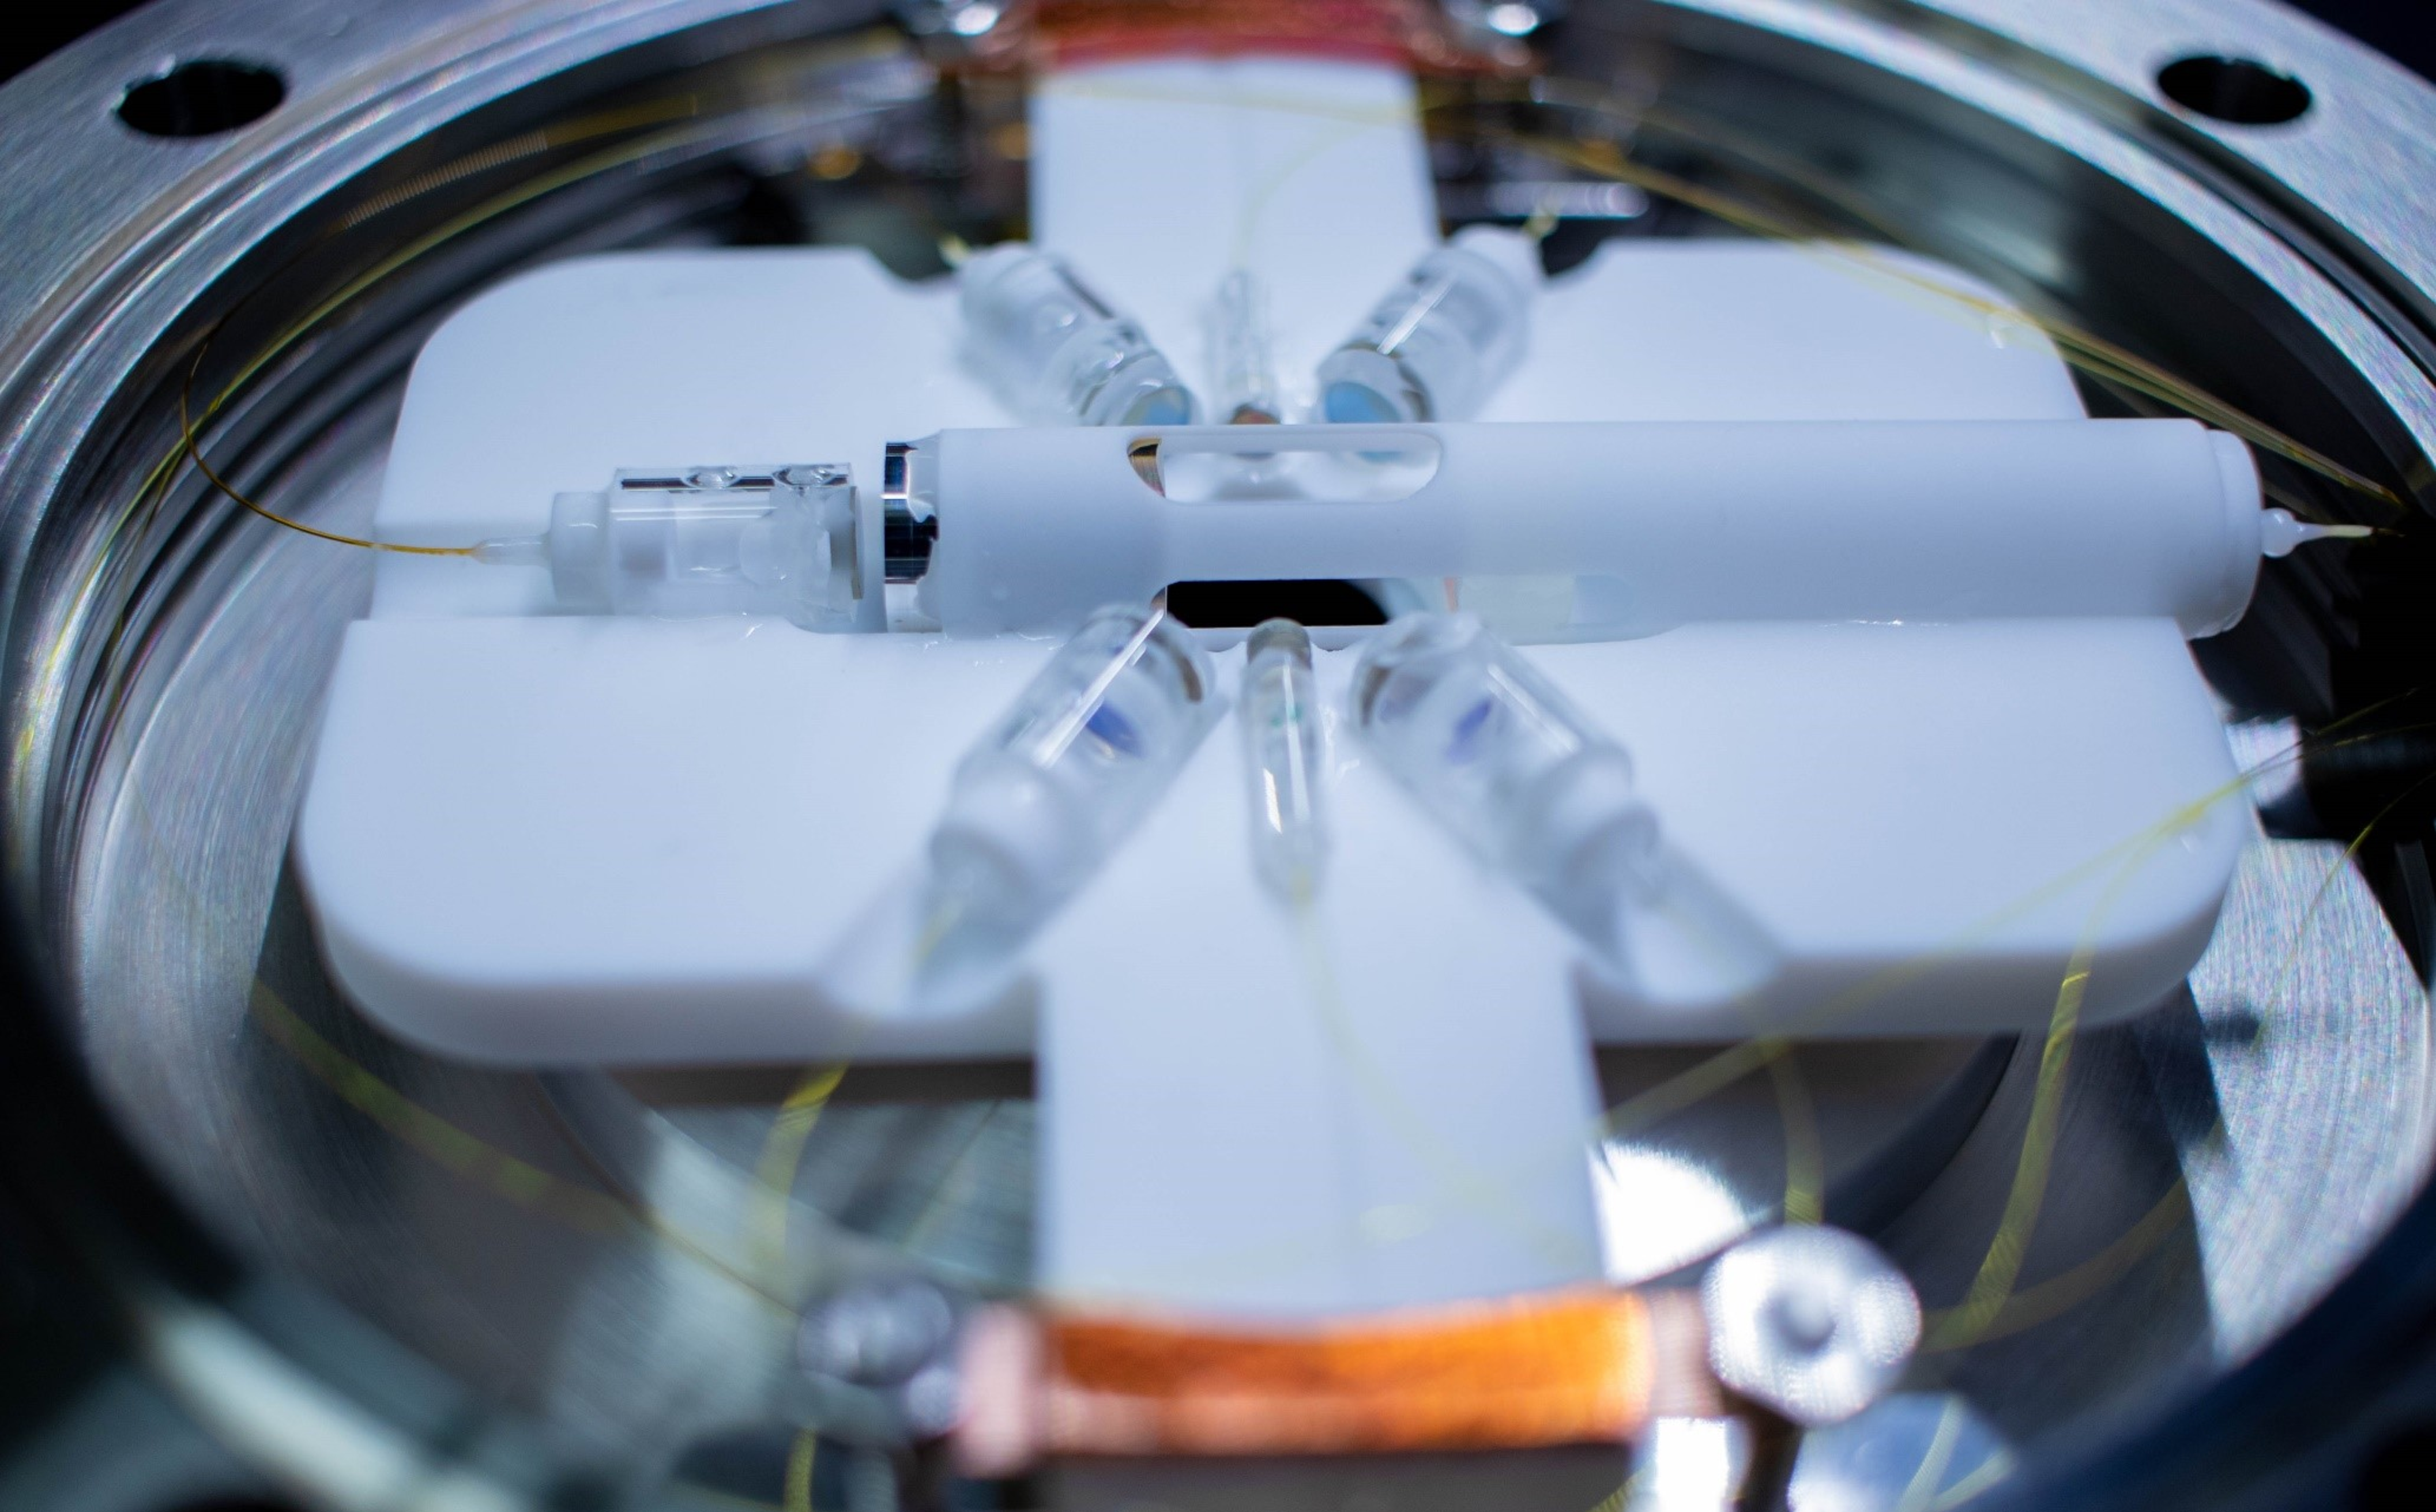
\includegraphics[width=\textwidth]{Images/chip_in_chamber_akbar.pdf}
    \end{subfigure}
    \begin{subfigure}[b]{0.375\textwidth}
        \centering
        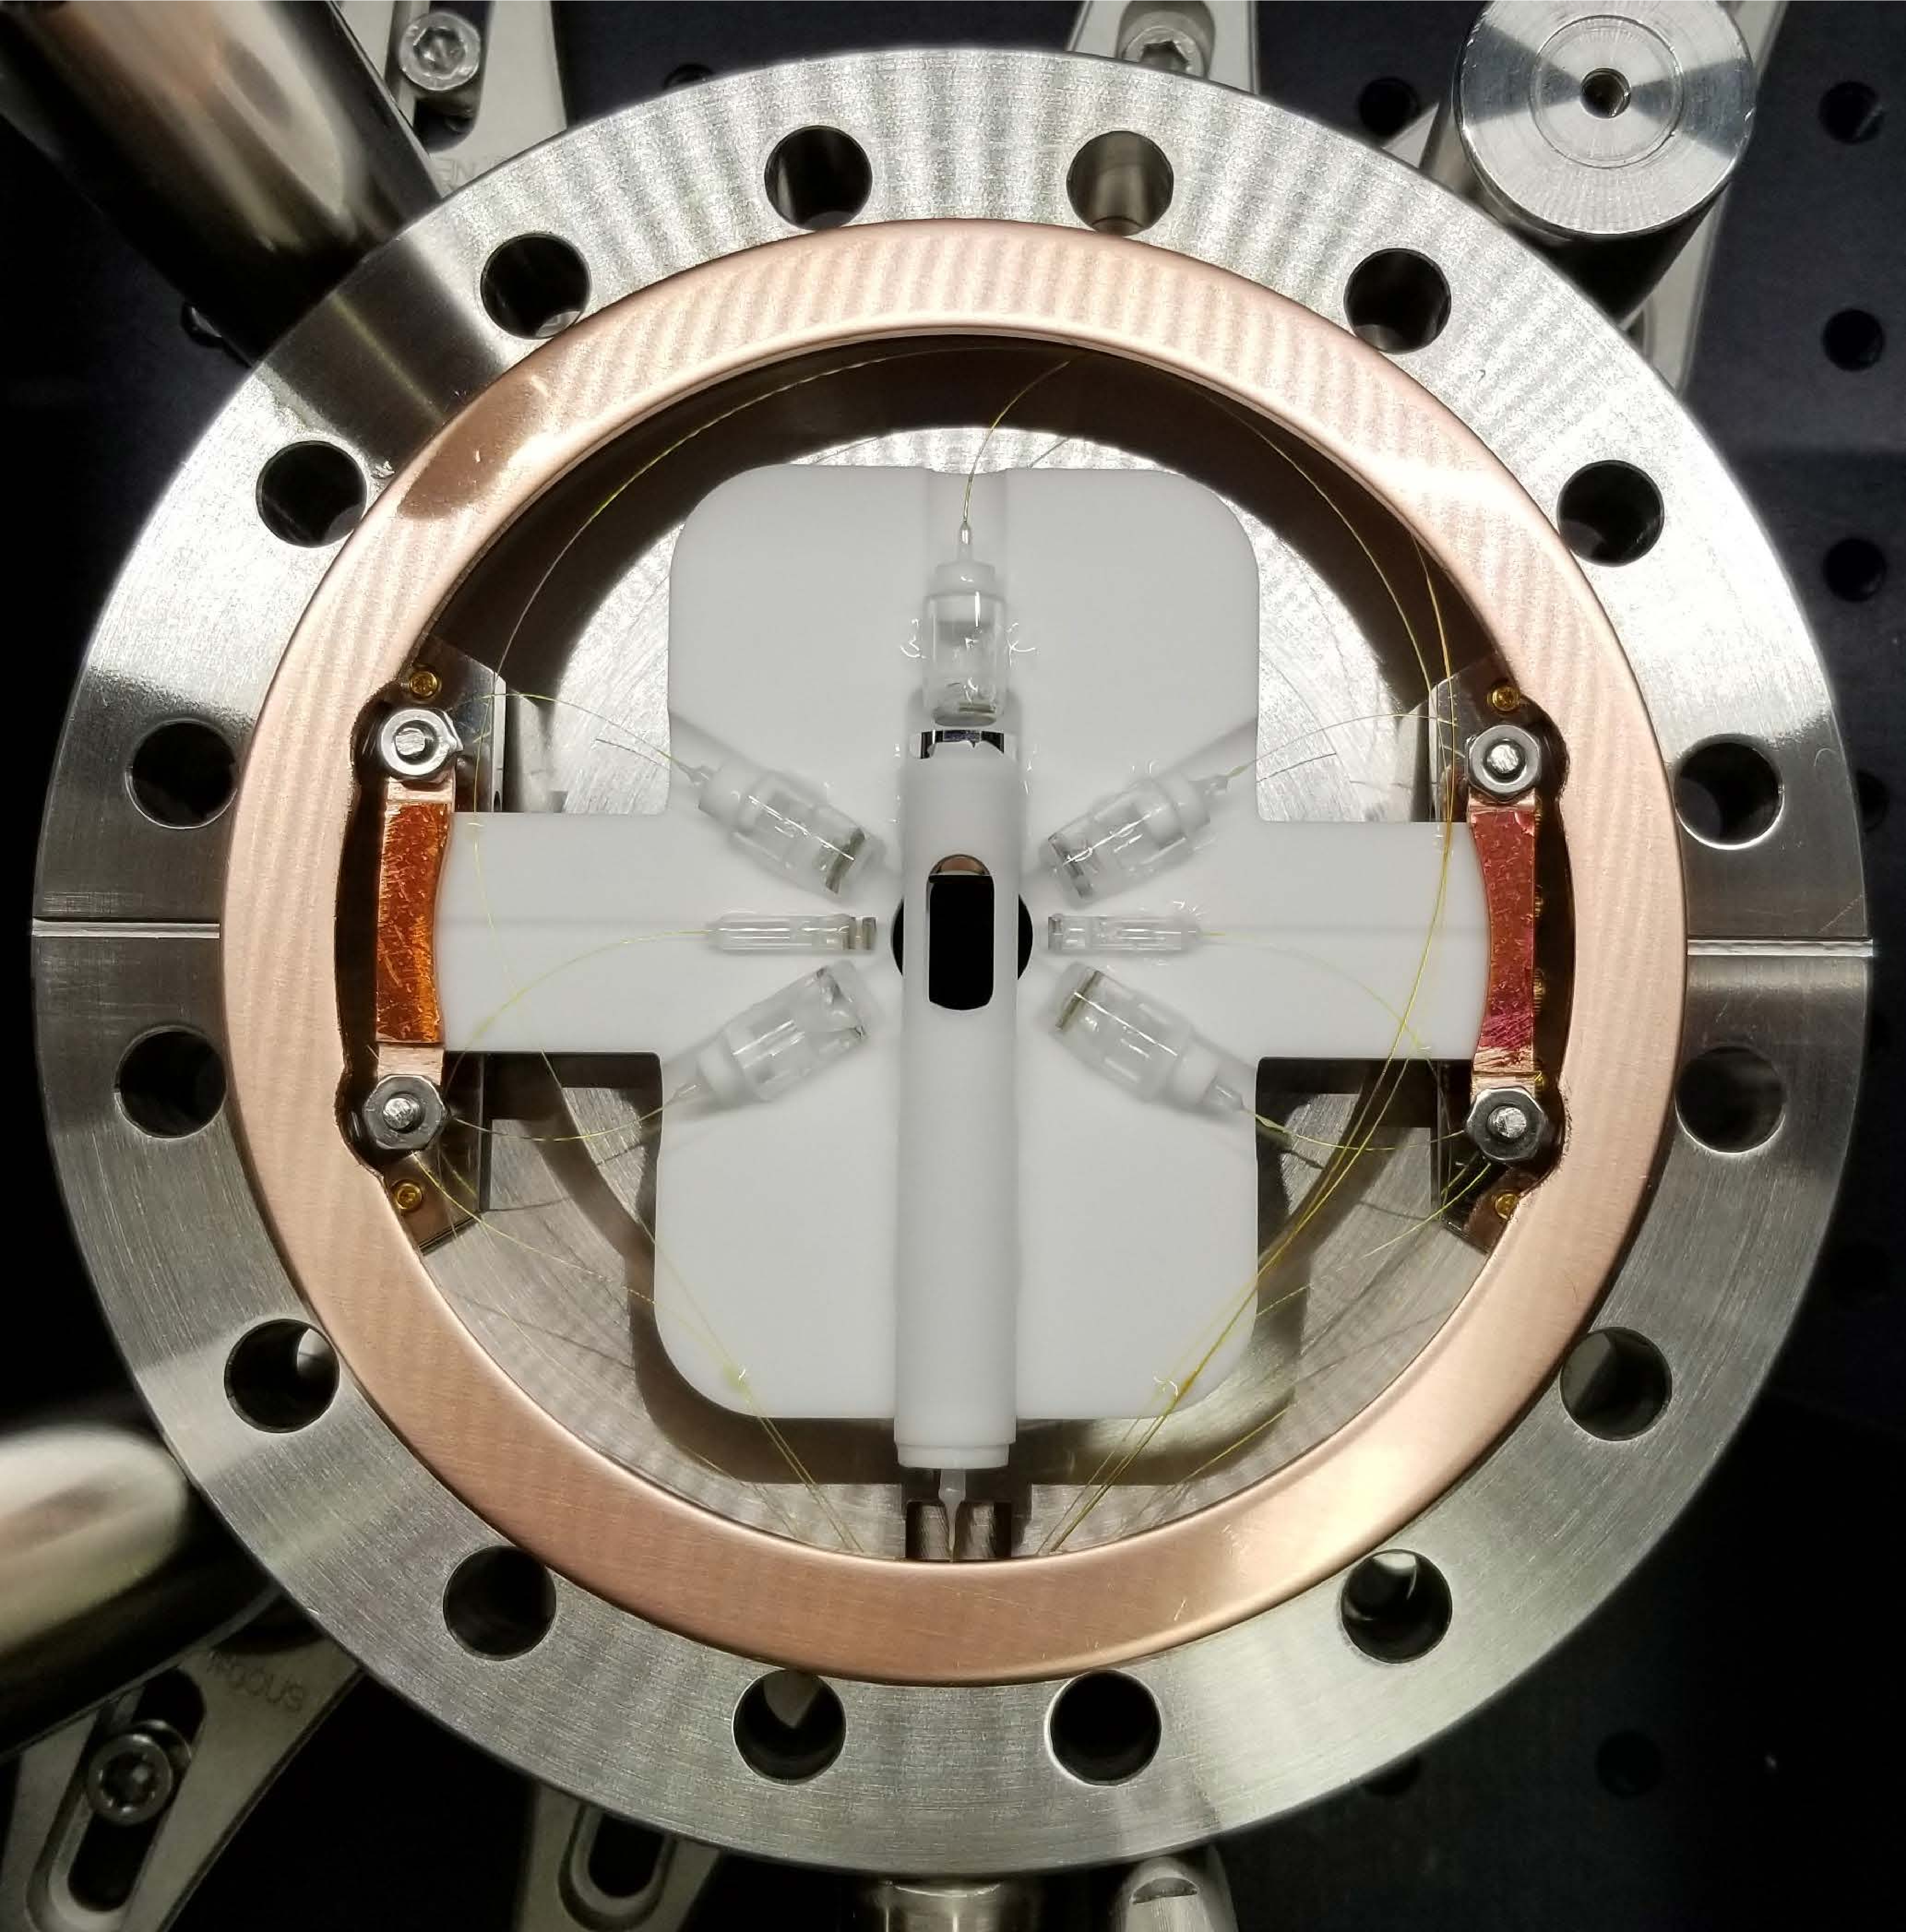
\includegraphics[width=\textwidth]{Images/chip_in_chamber_with_gasket.pdf}
    \end{subfigure}
    \hfill
    \caption{The finished optical chip in the science chamber, with the top of the chamber removed. In the right photo, note that the copper gasket has been cut to make clearance for the nuts which secure the bridge. Photo credit: Akbar Safari.}
    \label{fig:chip_in_chamber_akbar}
\end{figure}

As a final precautionary measure prior to installing the science chamber on the rest of the vacuum system, the chip was baked in air with the science chamber fully assembled. This was to ensure the glue, which can be cured with heat, was fully cured, allowing us to check the alignment of the optics a final time before the vacuum bake out. The chamber was ramped up to about 120 $^{\circ}$C at a rate of roughly 0.4 deg./min, and held at over 110 $^{\circ}$C for over an hour before being ramped back down to room temp. 

To check the final optical alignment after the air bake, the top of the chamber was removed and we mapped out the field of the beams using the tapered fiber scanning method described earlier. This time, we used a Femto FWPR-20-SI detector, which afforded us the sensitivity needed to detect light from the MOT and GRIN beams using only ~ 1 mW of injected power. A raster scan, as described in Sec. \ref{sec:mirror} was first used to verify that the shape of the parabolic mirror focal intensity had not become aberrated. Then, by first parking the fiber at the peak intensity of the mirror focus, a series of scans were done to check the relative positions of each beam with respect to the mirror focus. For MOT 1, MOT 4, GRIN 1, and GRIN 2, two 1D scans each were done, with one scan direction along the mirror optical axis, y, and the other, z, direction perpendicular to the Macor bridge. Scans were not done for MOT 2 and MOT 3, as coupling from 1 to 3 and from 4 to 2 was measured to be at least 7$\%$ and 2$\%$, respectively. Note that the actual coupling may be higher by a factor of two or so. This is because the light was butt-coupled into MOT 1 and MOT 4 using a fiber patch cord, and the efficiencies recorded use the power measured out of the patch cord, whereas we have observed a typical coupling between patch cord and connectorized fibers to be around 50$\%$.

The scans for the MOT beams and GRIN beams were done in increments of 100 $\mu$m and 50 $\mu$m steps, respectively, using the micrometer knobs on the NanoMax stage. Because of some hysteresis and user error on the order of 1 $\mu$m, after scanning away from the mirror focus along a particular direction, e.g. +Y , the fiber was re-centered on the mirror focus before continuing the scan direction -Y. The results of the scans are shown in Fig. \ref{fig:fiber_scan_post_airbake}, where it is apparent that the relative beam alignments are in agreement with the transparency sheet projections shown earlier in Fig. \ref{fig:final_beam_projections}. 

Following the final optical alignment check, the science chamber was sealed and connected to the rest of the vacuum system. After marking the end of each fiber with Sharpie to identify it, the connectors were snipped from the ends of the fibers to allow feeding them through the copper pinch-off tube, and subsequently, the fiber feedthroughs. Then, with the aid of a piece of copper sheet bent in the shape of a funnel and inserted into the neck of the pinch-off tube.


\section{Lasers}

Lasers of several frequencies are needed in the quantum network experiment for cooling, trapping, imaging, exciting, and pumping atoms into various internal electronic states. These different frequencies are shown in Fig. \ref{fig:laser_frequencies}. The lasers used supply power to both network nodes, i.e., each individual laser head has its power split between both nodes. This has the advantage that any intensity noise present directly on the laser output is common mode and could be mitigating with only one feedback loop upstream of the split. It also allows the possibility of reducing the number of AOMs required to the pulse the lasers once the two nodes are operating together as a network rather than as indepenedent systems. A schematic with all of the quantum network lasers is given in Fig. \ref{fig:all_lasers_schematic}. 
\begin{figure}[h!]
    \centering
    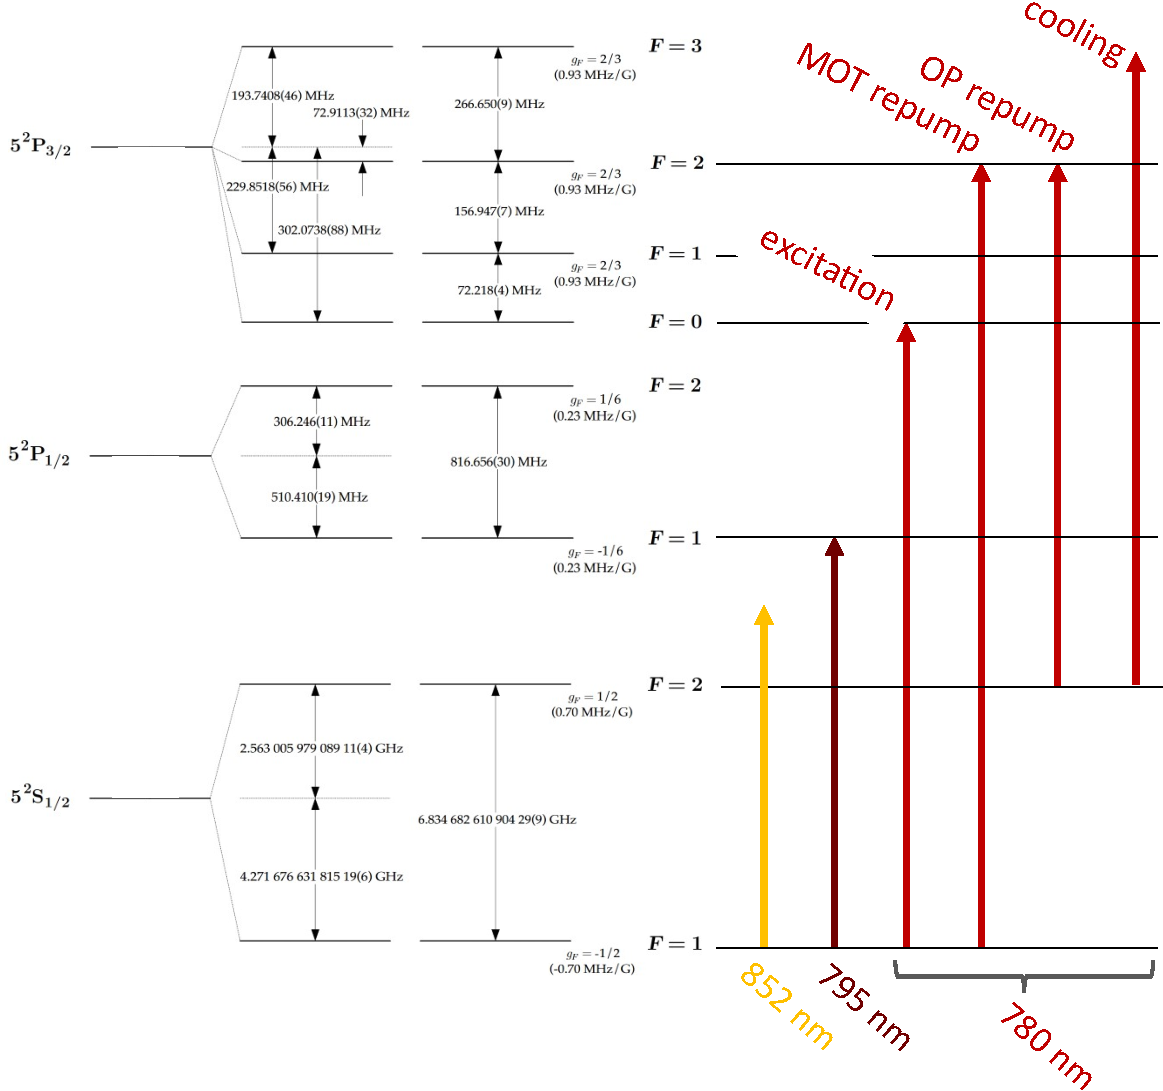
\includegraphics[width=0.9\textwidth]{Images/laser_frequencies.pdf}
    \caption{The different laser frequencies used in the quantum network experiment and their purposes.}
    \label{fig:laser_frequencies}
\end{figure}

\subsection{D2 Line cooling, excitation, and repumpers}

There are four laser frequencies with a nominal wavelength of 780 nm which we generate using only two distributed-feedback (DFB) laser sources (Eagleyard DFB Eagleyard EYP-DFB-0780-00080-1500-TOC03-0005) plus AOMs for frequency shifting. The two lasers supply two frequencies each, divided up by whether the relevant frequency is closer to resonance on the $D_2$ line with $F=1$ or $F=2$ in the ground state. In particular, one laser is locked on $F=1 \leftrightarrow F'=0$ and used to generate the excitation light (for generating single photons from the atoms) and the MOT repumper, while the other is locked on $F=2 \leftrightarrow F'=3$ and used for cooling/imaging and optical pumping (OP) repumper. Both lasers are locked using homebuilt saturated absorbtion setups in modulation transfer spectroscopy (MTS) configuration and homebuilt lockboxes.

The power of the individual DFB laser heads is insufficient for supplying power to both nodes, so each seeds a tapered amplifier (TA) for additional power. The cooling laser uses a homebuilt TA setup (with Eagleyard EYP-TPA-0780-03000-4006-CMT04-0000 TA chip) based on the design in \cite{kangara2014design}. The excitation laser seeds a commercially available fiber-coupled TA solution (MOGLabs MOAL with 785TA3000D TA chip) which provides over 1 W after the output fiber.

\begin{figure}[h!]
    \centering
    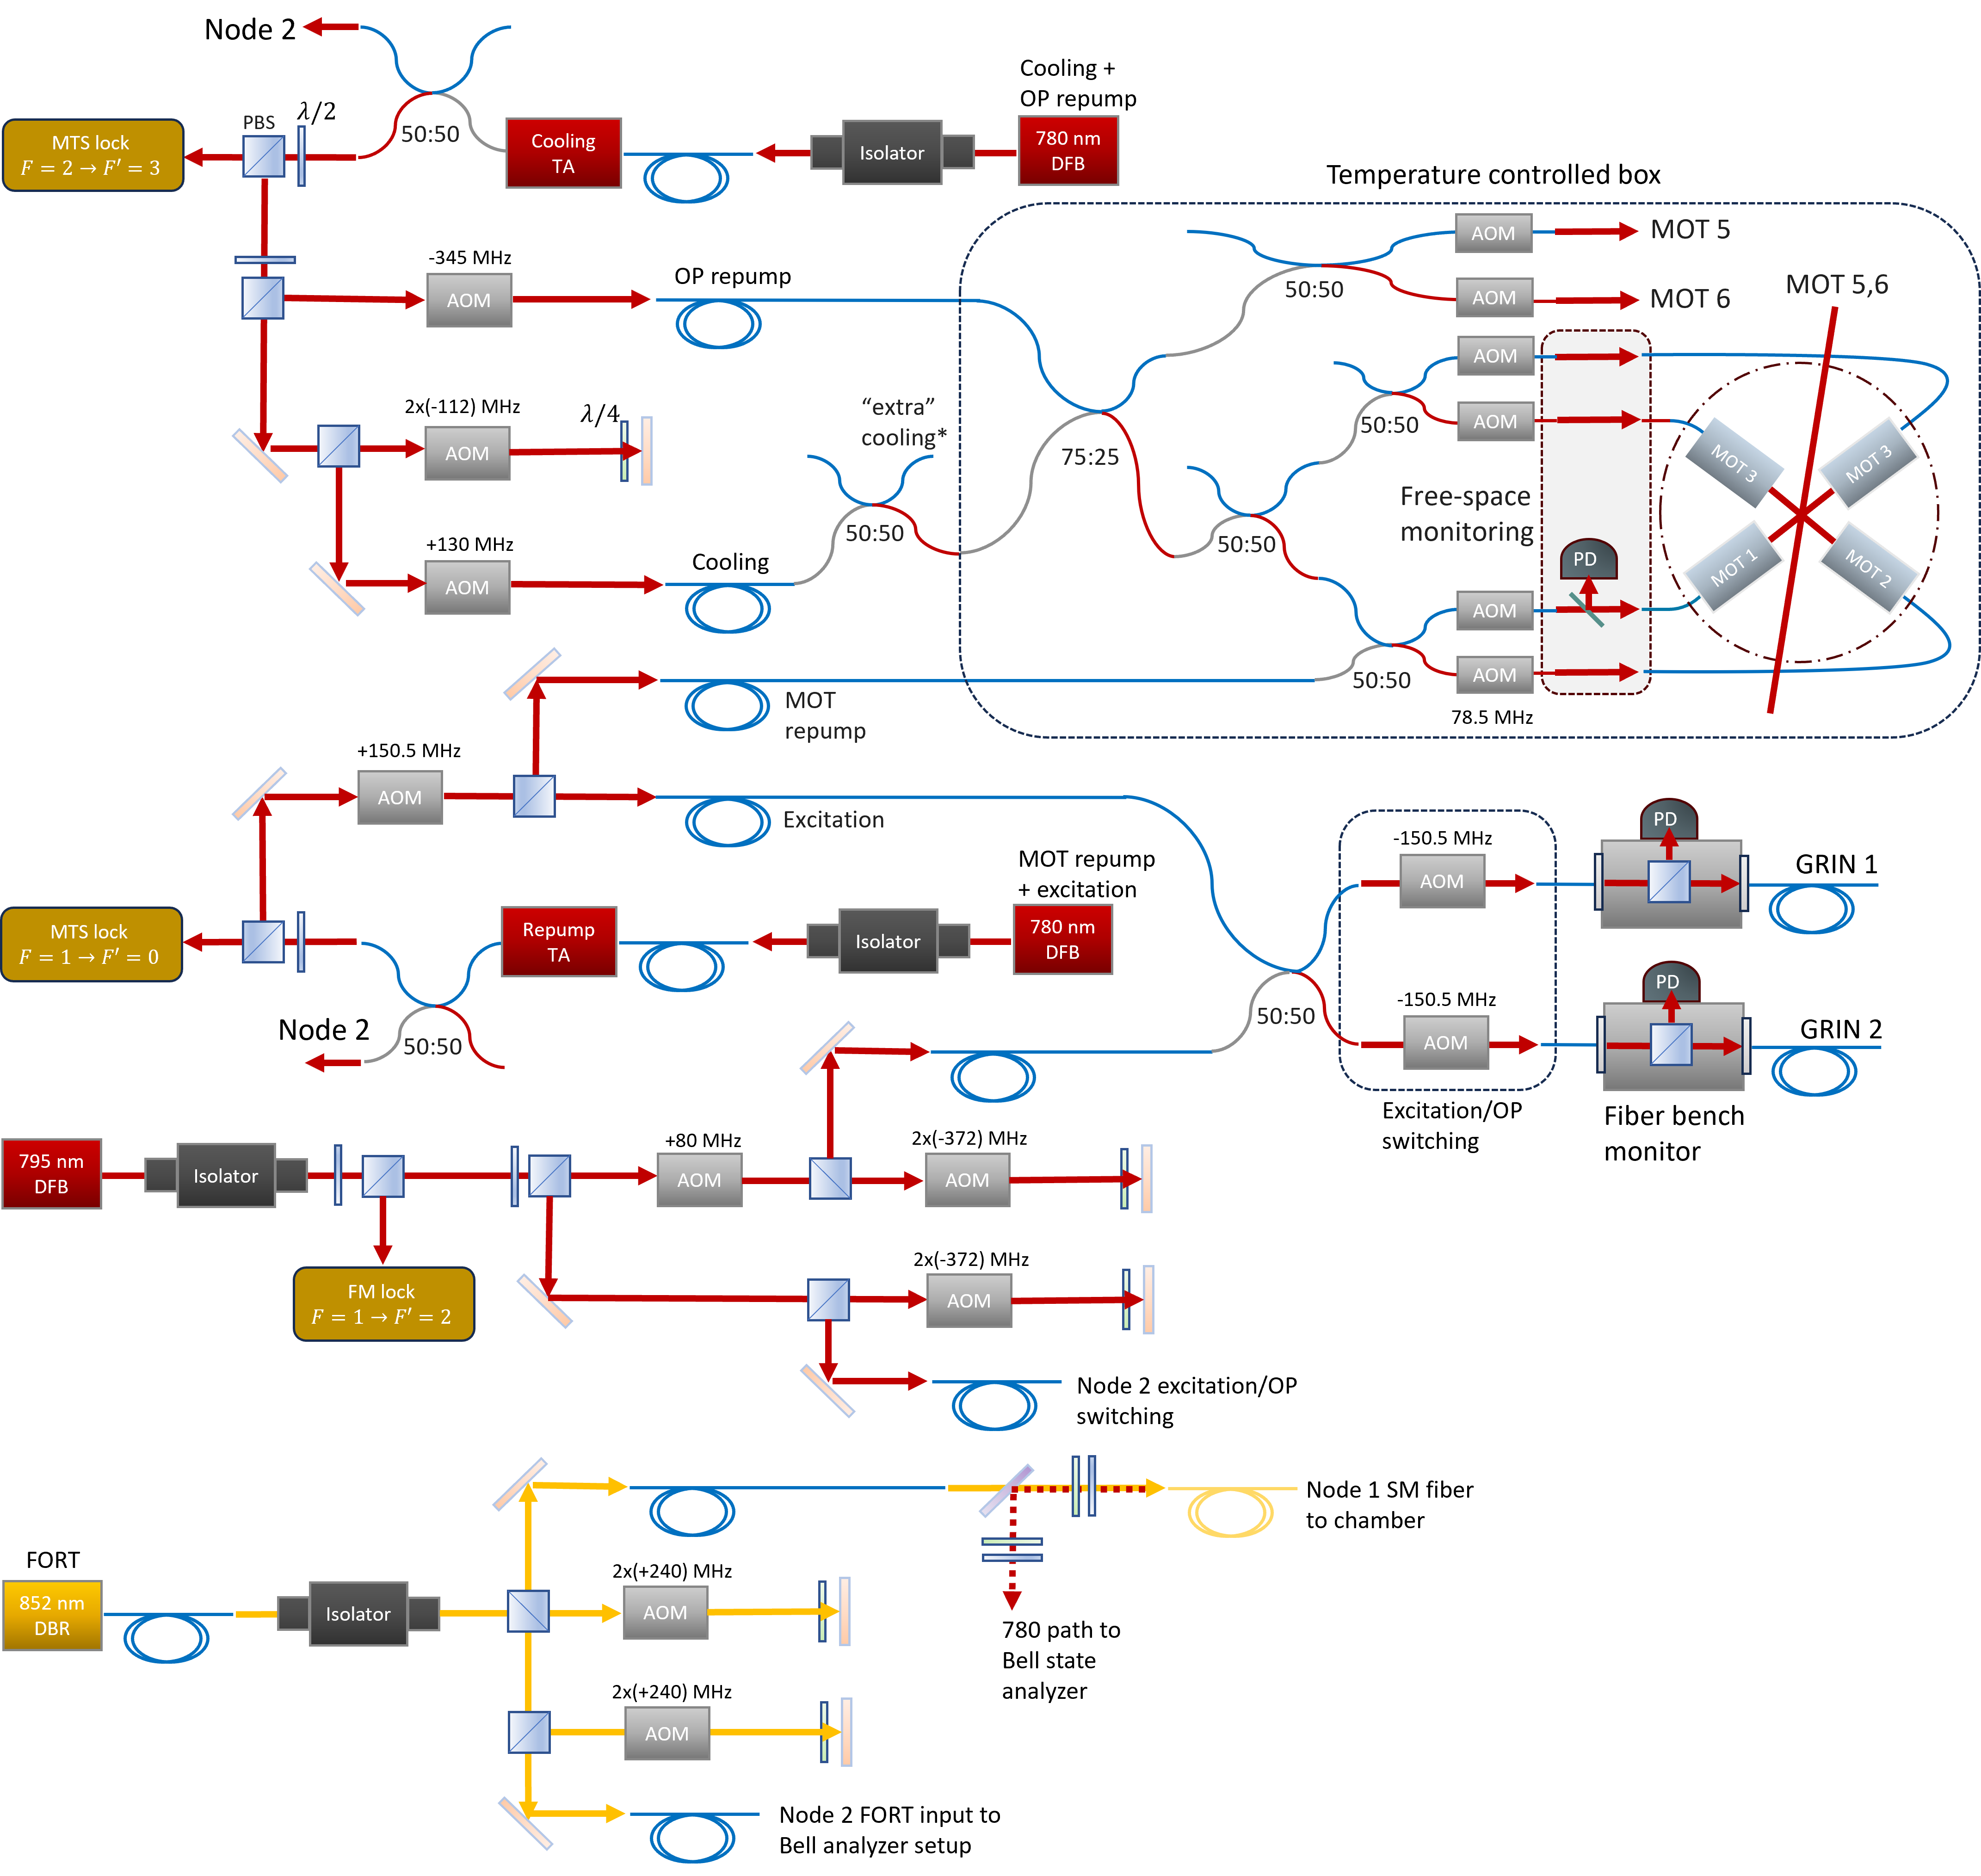
\includegraphics[width=0.9\textwidth]{Images/quantum_network_lasers_schematic.png}
    \caption{Schematic of the laser systems and routing for the quantum network experiment. Each laser head supplies both nodes, but only the common paths and those for one node (arbitrarily chosen to represent Node 1). The Node 2 setups are mostly duplicates of those for Node 1 except for some minor component-level differences.}
    \label{fig:all_lasers_schematic}
\end{figure}

The cooling, MOT repump, and OP repump are delivered to the science chamber's fibers through a fiber breakout made from PM fiber splitters (Thorlabs) linked with with PM butt connectors. Fiber-connectorized AOMs (CSRayzer AOM-780-78.5M-05-S-C1-PM780-1-1-1-FA) are used for introducing small frequency differences between MOT beams for standing wave mitigation, as well as switching of the MOT beam paths and performing dc intensity stabilization (see Sec. \ref{sec:fiber_AOM_power_stabilization}). 

\subsection{D1 Line optical pumping}

A 795 nm DFB laser (EYP-DFB-0795-00080-1500-TOC03-0005) resonant with $F=1 \leftrightarrow F'=1$ on the $D_1$ line is used for optically pumping the atoms into $\ket{F=1, m=0}$. The laser is locked on the $F=1 \leftrightarrow F'=2$ $D_1$ transition with frequency modulation (FM) saturated absorption spectroscopy and frequency shifted with AOMs. This light shares a path to the atoms with the excitation light, where two AOMs are used for switching between two opposite directions (GRIN 1 and GRIN 2 paths in the chamber). This choice was made  because alternating between the two paths during optical pumping can reduce photo-scatter induced heating \cite{su2024fast}.

\subsection{FORT}
The dipole trap or far-off resonant trap (FORT), which we use interchangeably, is formed with a high-power 852 nm distributed Bragg reflector (DBR) laser (Photodigm 852.347DBRH-IBragg). The FORT light is coupled into the SM fiber interface to the science chamber after being combined with the 780 nm photon path using a dichroic beamsplitter (AVR Optics LPD02-785RU-25).  

\section{Magnetic field coils}
The coils for creating the quadrupole field for forming a MOT as well as shim fields and a bias field for entanglement experiments were made from Kapton-coated wire wrapped around custom aluminum holders designed by the author (Fig. \ref{fig:node1_coils.pdf}). The holders consist of six c-shaped sections, one for each coil which bolt to each other to form a frame which clamps to the chamber. The c-shape, rather than a closed loop, was chosen to mitigate the formation of eddy currents. The author notes that in retrospect, a non-metallic material or a variant of this design with fewer sharp edges would be preferable in a future build, as multiple shorts in the wires were found after wiring, apparently caused by the Kapton coating being worn off in certain places during the winding process. The version of coil holders used in the second node still suffered from this problem, despite design changes to reduce the number of edges encountered by the wires during winding.

\begin{figure}[h!]
    \centering
    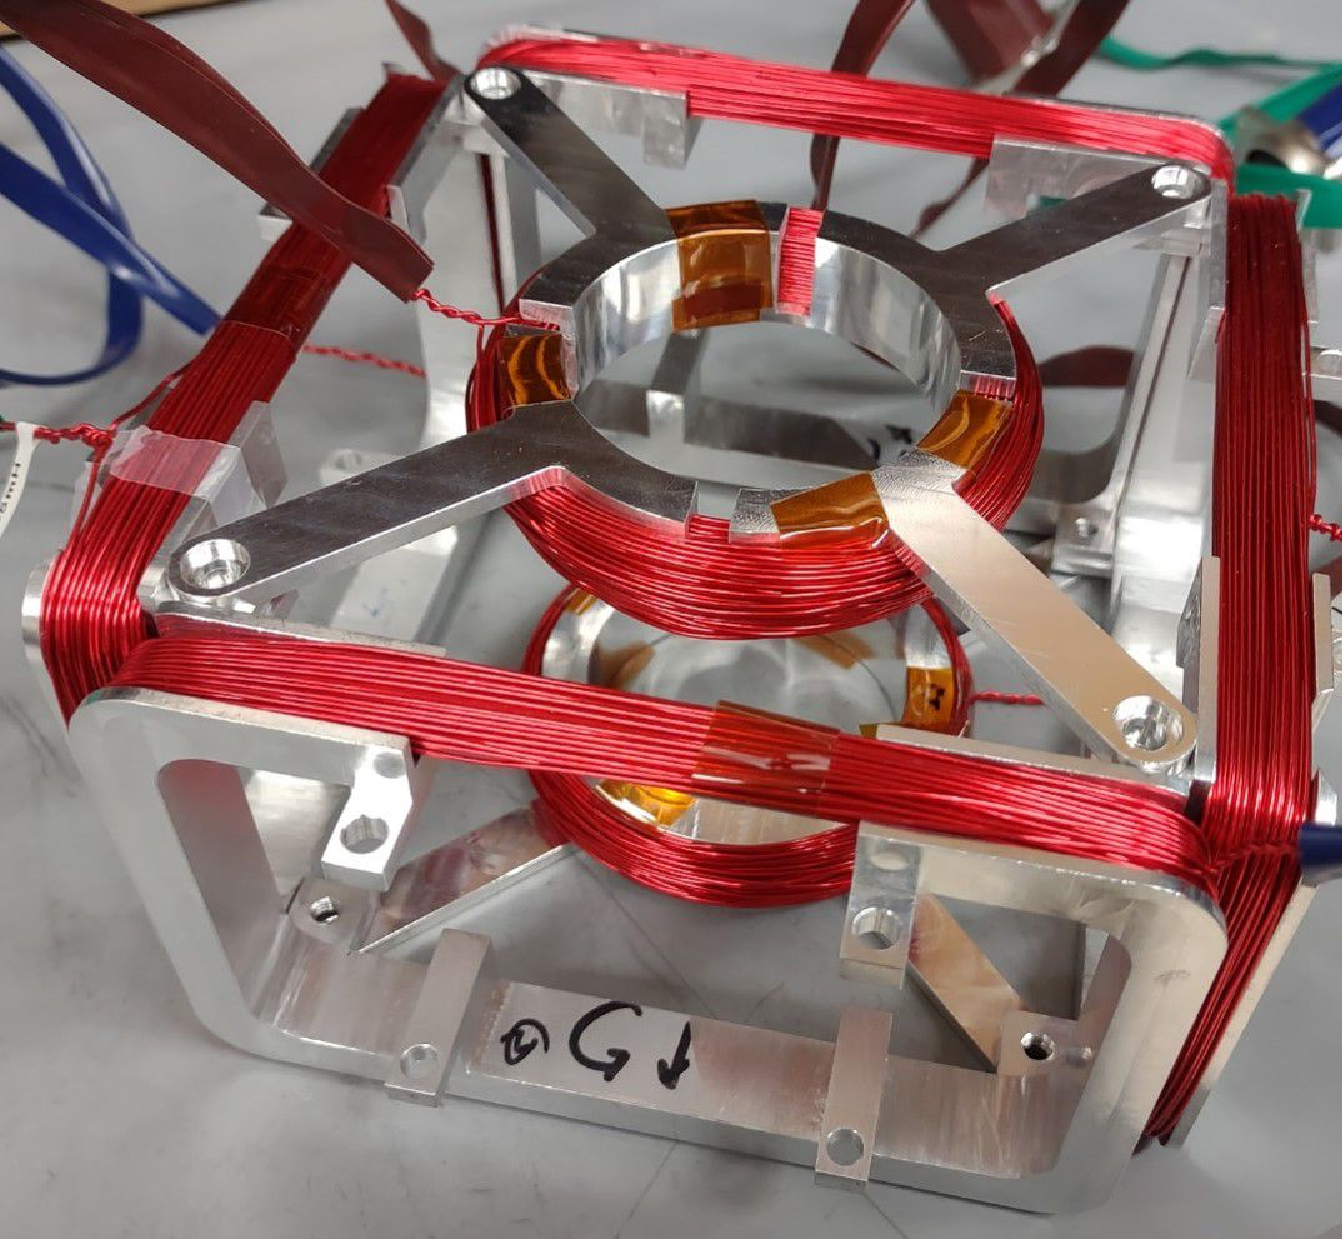
\includegraphics[width=0.7\textwidth]{Images/node1_coils.pdf}
    \caption{The coil assembly used for the first version of the quantum network experiment. A second version with minor modifications was made to give slightly deeper channels for the coils and notches to help start the winding. The circular coils can be driven in either an anti-Helmholtz or Helmholtz configuration to form a quadrupole field for the MOT or shim fields, respectively.}
    \label{fig:node1_coils.pdf}
\end{figure}

More details on preliminary coil testing will be given in the upcoming PhD thesis by Eunji Oh. Details on the design of the home-built coil drivers might be given in the upcoming PhD thesis by Jacob Scott. 

% \section{MOT Geometry}

% ?? section needs fixing, particularly the equations. otherwise, omit entirely

% The MOT geometry in the parabolic mirror version of the network node has no pairs of orthogonal beams among the three pairs, which is a result of the requirements imposed on the geometry by the in-vacuum optics and external objective lenses (see Fig. (\ref{fig:chamber_cross_section})). MOTs have been demonstrated with angles much less than 90 degrees between beam pairs (\cite{Garcia2013}), but the relative optical intensity in different pairs must be tuned to give comparable force gradients in each Cartesian direction.

% \begin{figure}[h!]
%     \centering
%     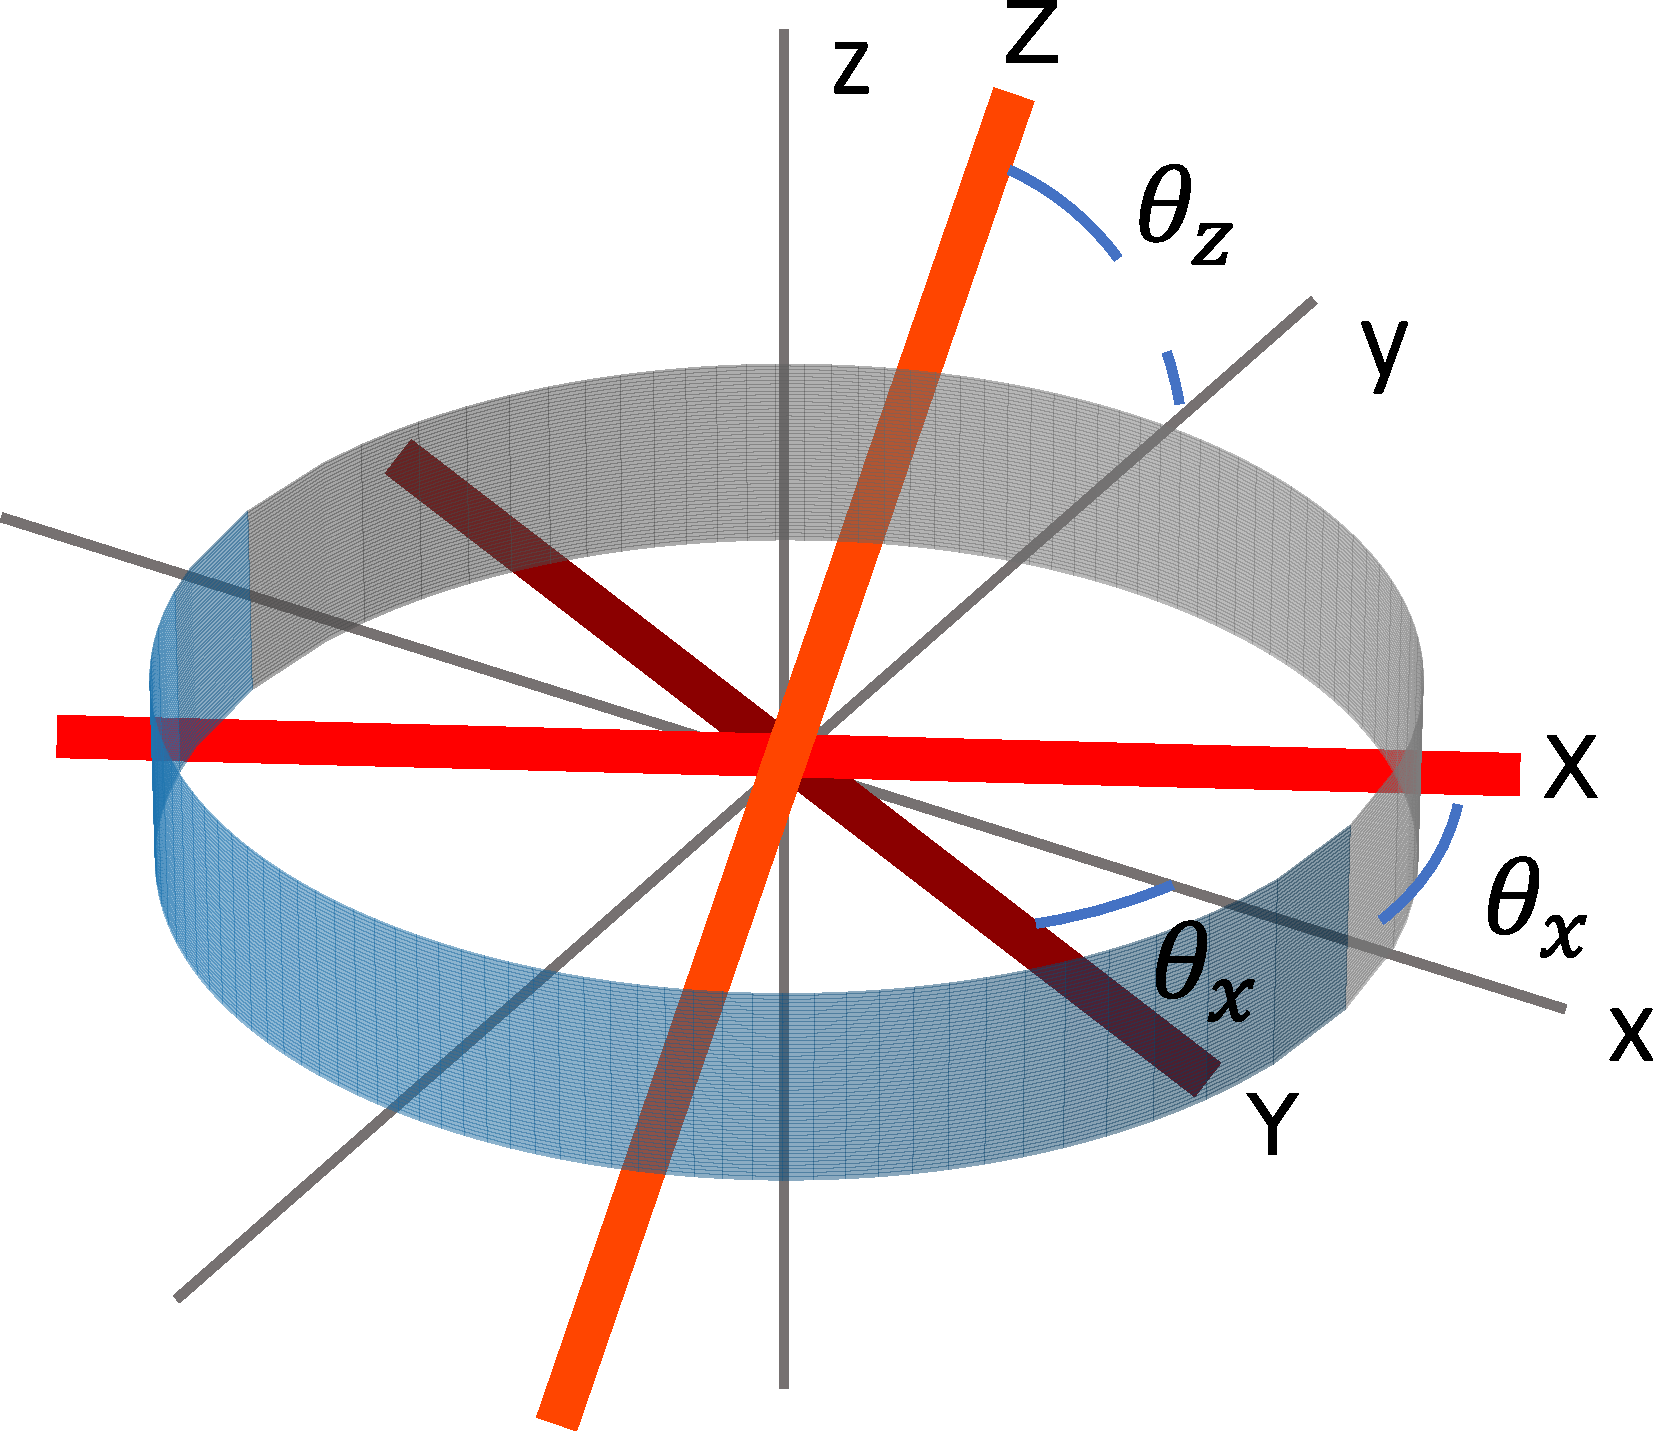
\includegraphics[width=0.5\textwidth]{Images/goofy_mot_beams.pdf}
%     \caption{Non-orthogonal pairs of MOT beams. The cylindrical shell is intended to invoke a notion of where our vacuum chamber would be with respect to this set of beams. ?? double check this graphic}
%     \label{fig:goofy_mot_beams}
% \end{figure}

% Consider a MOT with beam pairs X, Y, and Z, where X and Y lie in the $x-y$ plane and Z lies in the $y-z$ plane, with angles $\theta_x$ between the X/Y beams and the $x$ axis, and $\theta_z$ between Z and the $z$ axis, as in Fig. \ref{fig:goofy_mot_beams}. The two-level atom radiative force including the detuning of the light $\delta$ and Zeeman shift $\Delta_B$ due to a magnetic field due to a pair of beams $i$ is, in a low-intensity approximation, given by
% \begin{equation}
%     F_i(\mathbf{r}) = \frac{s_i}{1 + s_i + 4(\delta + \Delta_B(\mathbf{r}) \hat{B}(\mathbf{r})\cdot\hat{e}_i)^2/\gamma^2} - \frac{s_i}{1 + s_i + 4(\delta - \Delta_B(\mathbf{r}) \hat{B}(\mathbf{r})\cdot\hat{e}_i)^2/\gamma^2}
% \end{equation}\label{eq:force_i}
% where $\hat{B}\cdot\hat{e}_i$ gives the dot product of the magnetic field at a particular point in space with the propagation axis of the beams and $s_i$ is the saturation parameter, assumed to be equal for both beams in the pair. For the beams denoted X,Y, and Z as defined, the forces along Cartesian directions $\hat{x},\hat{y}$ and $\hat{z}$ are
% \begin{align}
%     F_x &= F_X \cos{\theta_x} + F_Y \cos{\theta_x} \\
%     F_y &= F_X \sin{\theta_x} + F_Y \sin{\theta_x} + F_Y \sin{\theta_z} \\
%     F_x &= F_Z \cos{\theta_z}
% \end{align}
% where the $F_i$ on the RHS are given by Eq. (\ref{eq:force_i}). In order to find beam intensities which give a symmetric MOT in $\hat{x}$ and $\hat{y}$, we can find solve the system 
% \begin{align}
%     \nabla F_y &= \nabla F_x \\
%     \nabla F_x &= -\kappa \nabla F_z \\
%     s_x &= s_y
% \end{align}
% for $s_y, s_z$, and $\kappa$, evaluated at $x=y=z=0$, where $\kappa$ is a positive-valued constant. We can approximate the magnetic quadrupole field by $B = B_0 (-x/2 \hat{x} -y/2 \hat{y} + z\hat{z})$

% If the radiative force including the spatially-dependent Zeeman shifts along the $i^{\textrm th}$ beam pair is $f_i$, we can compute the forces $F_{i}$ along each Cartesian axis $i$: ?? not correct

% \begin{align}
%     F_x = f_x \cos(\theta_x) + f_y \cos(\theta_x) \nonumber \\
%     F_y = f_x \sin(\theta_x) + f_y \sin(\theta_x) + f_z \sin(\theta_z) \\
%     F_z = f_z \cos(\theta_z) \nonumber
% \end{align}

\section{Experiment Control}

Quantum networking experiments with cold atoms require control hardware including analog and digital inputs and outputs, each with a high degree of timing precision. It is also important to be able to write flexible control programs which streamline experiment runs, including data acquisition and analysis. For these purposes, we use the Sinara hardware suite and ARTIQ control software. Our Sinara hardware consists of analog and digital I/O and DDS channels controlled by a Zynq-based FPGA controller, the Kasli-SoC\cite{lam2021combining}. The benefit of FPGA-controlled hardware, as opposed to looping a predetermined pulse sequence, is the ability to have experiments with conditional logic which determines how the experiment progresses. This is particularly important for the probabilistic entanglement sequence described in Sec. \ref{sec:reg}, in which a detection event heralding remote entanglement can be used to break out of the entanglement attempt loop to use the entanglement as a resource. Breaking out of the loop is also a necessity for verifying the state with quantum state tomography and for reloading atoms when one is lost.

For one-node operation described in this thesis, each network node is independently controlled by its own Sinara hardware and ARTIQ instance. However, for two-node operation, the FPGA controllers (Kasli-SoC) can be operated in a satellite configuration in which one operates as a master while the other(s) follows and the two share a clock \cite{Stephenson2020}. 

% could make a figure showing how many channels are controlling each thing?
% \part{Experiment}\label{part:experiment}
\chapter{Preparation, manipulation, and measurement of neutral atom qubits}\label{ch:qubit_prep}

\section{MOT}
% finding the "first" MOT, with Z beams at the angle we use.
% say things about the typical size of the MOT, include pictures
% of bright MOTs we've gotten. alignment of the z beams to the 
% repump. signal of the MOT with the SPCM vs magnetic field 
% parameters? reference a figure of the switchyard schematic, which
% we can put in the lasers section
\subsection{Alignment and imaging}

Laser cooling and spatial confinement of atoms in a magneto-optical trap (MOT) is the first step in preparing neutral atom qubits, as individual atoms can then be trapped from the cloud of cold atoms in the MOT. The network experiment MOTs are loaded from a background vapor from a Rb ampule with a naturally occurring isotope ratio.

The first MOT found in network Node 1 used external MOT beams which were perpendicular to the chamber windows for ease of alignment. However, future experiments including atom array and Rydberg experiments require the use of an external objective lens, and we
send the external beams in at an angle of $35^{\circ}$ to the normal to bypass this objective. This reduces complications which would arise from sending the external MOT beams through the same path used for imaging array atoms, such as heating due to the inability to have three-dimensional cooling while imaging. We note that there are ways to mitigate this kind of issue, but they are often atomic species dependent\cite{covey20192000}.

The alignment of the external MOT beams to those on-chip is necessary to form a MOT,
but tricky due to the lack of optical access from the side of the chamber. Alignment is additionally complicated due to severely limited clearance ($\leq$ 1 mm) at the edge of the 0.4 NA objective lens (custom, JenOptik) mounted at the bottom chamber window. This limitation is shown clearly in Fig. (\ref{fig:chamber_cross_section})
\begin{figure}[!ht]
    \centering
    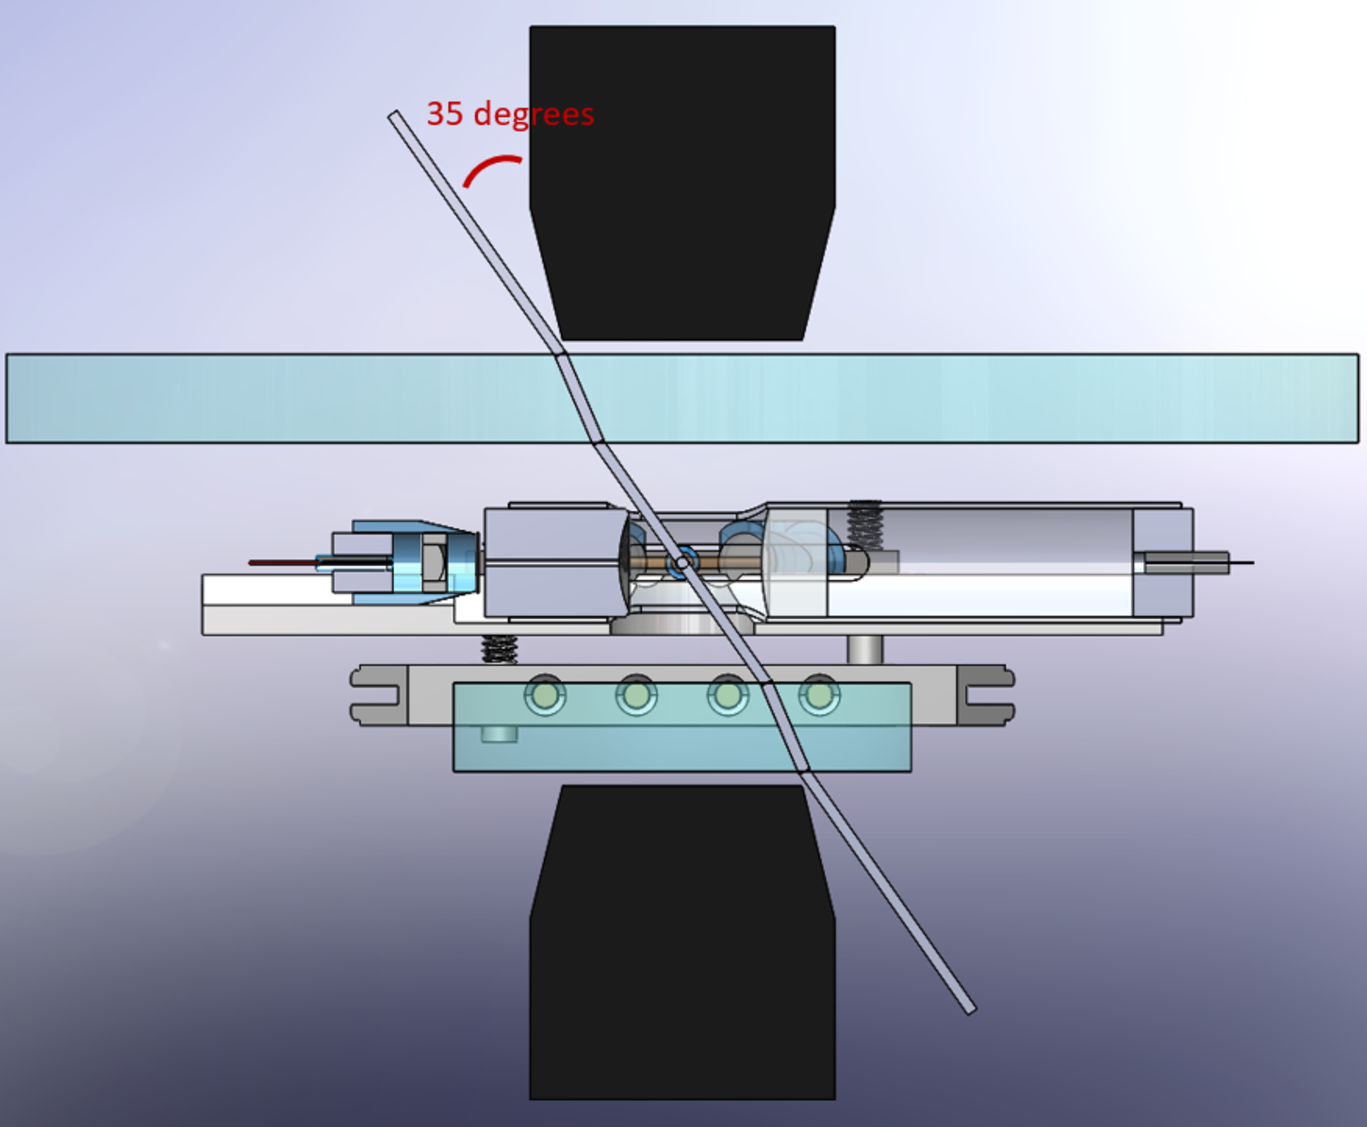
\includegraphics[width=0.9\textwidth]{Images/chamber_cross_section.pdf}
    \caption{Cross section of the network node science chamber, with the steel chamber hidden, with two 0.4 NA JenOptik objectives represented in black. The cylindrical solids representing the MOT beam have radius equal to the $1/e^2$ intensity waist $w_0$, and there is $\sim~2w_0$ from the beam axis to the objectives at closest approach.}
    \label{fig:chamber_cross_section}
\end{figure}
We overcame the limitation of optical access by using the atomic fluorescence to verify proper MOT beam alignment. By launching resonant MOT repump light through one of the on-chip MOT beams, and sending only cooling light through the top external MOT beam, we were able to align the top MOT beam until there was an obvious increase in fluorescence where the beams overlapped, as seen by imaging with an Andor Luca camera from the top chamber window. For this technique be reliable, it is necessary to make sure there is negligible fluorescence from the repump itself, which would result in an increased fluorescence signal near the overlap region even if the beams are not crossing. The camera settings must also beadjusted to clip the image so background, e.g. from scattering in the chamber, does not obscure the signal. The beam overlap can then be clearly verified by moving the repump on and off resonance, as shown in Fig. (\ref{fig:external_beam_alignment}).
\begin{figure}[!ht]
    \centering
    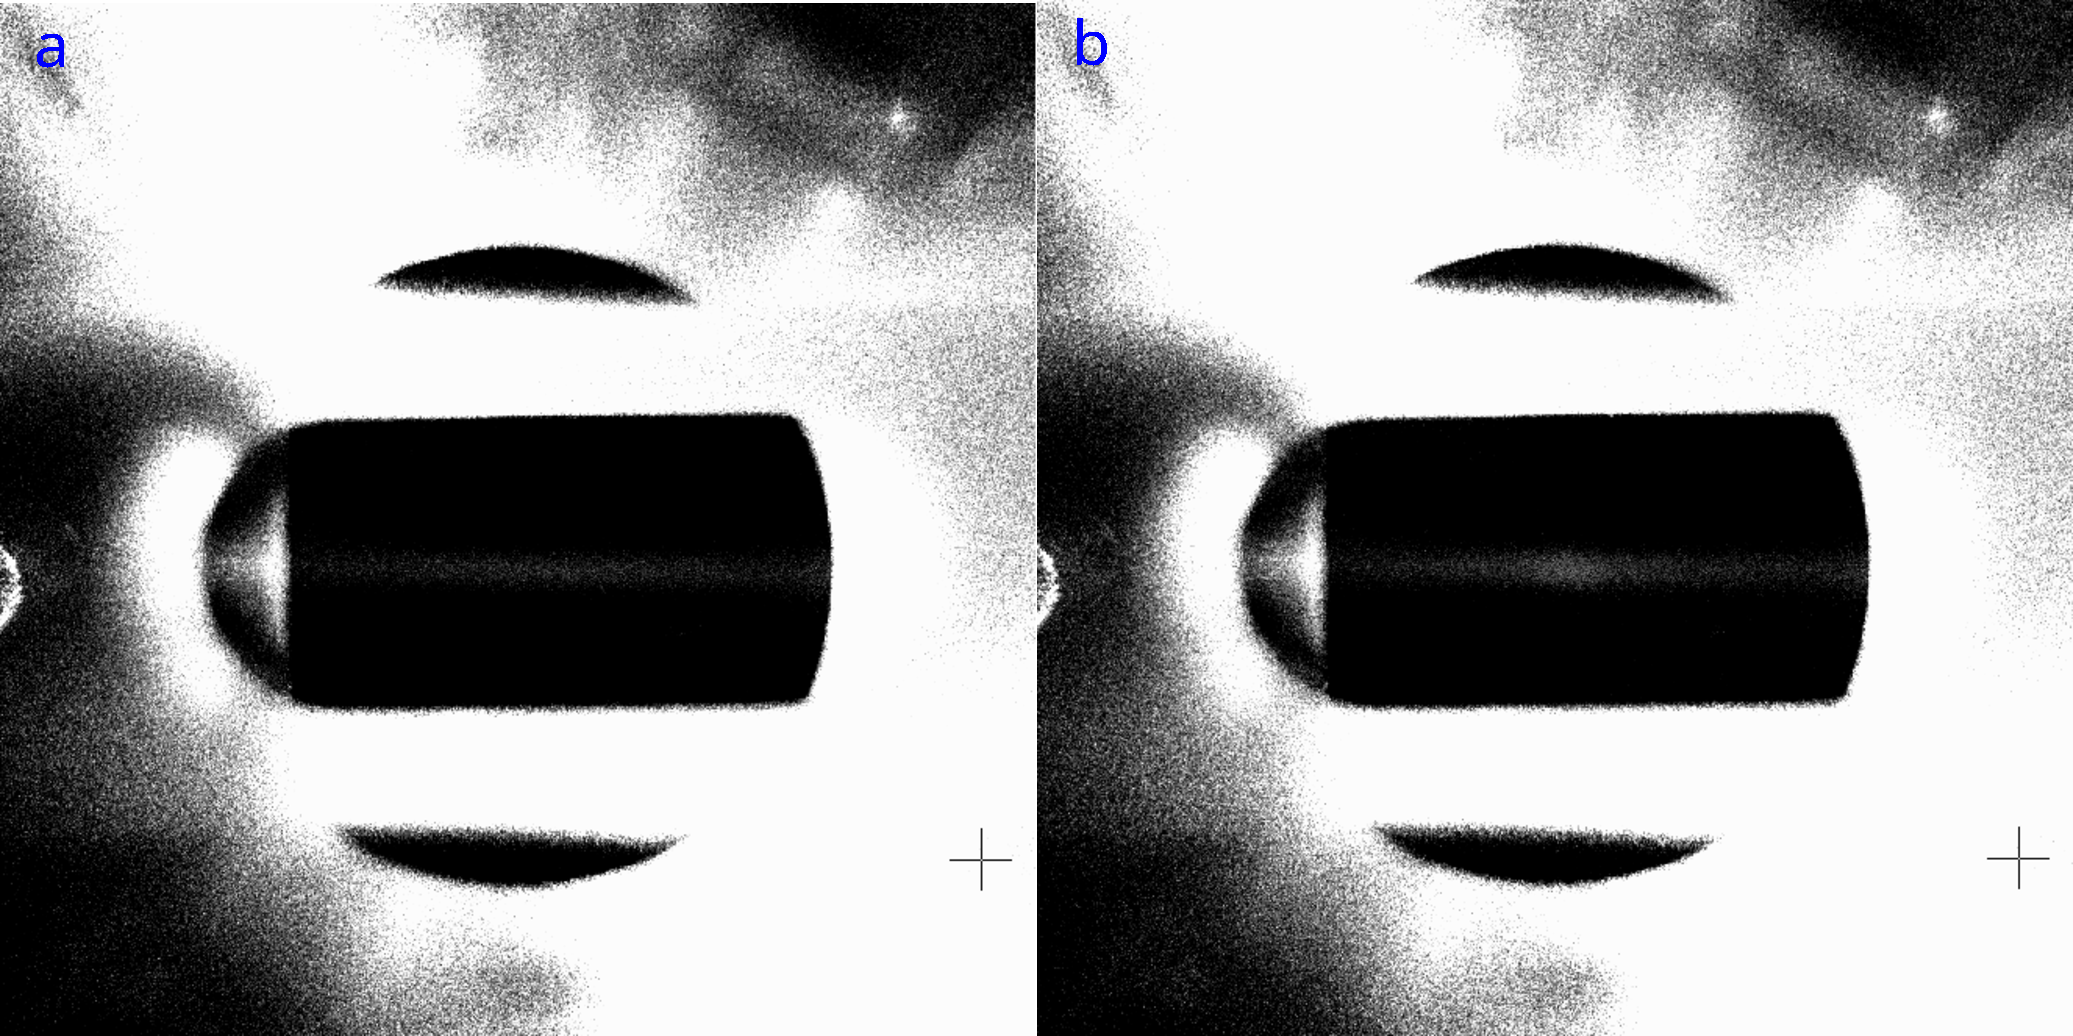
\includegraphics[width=0.9\textwidth]{Images/mot6_alignment_to_repump.pdf}
    \caption{Alignment of the MOT6 beam, containing only cooling 
    light, to an on-chip beam containing only MOT repump light. When the 
    beams are overlapped and the cooling laser is (un)locked as in \textbf{b} (\textbf{a}) there is (isn't) a clear enhancement of the 
    fluorescence in the region of overlap.}
    \label{fig:external_beam_alignment}
\end{figure}
The bottom external beam can then be aligned to overlap the top beam, for example by coupling it into the top beam fiber. Finally, two things are important to note regarding this alignment procedure. 1) While we were able to find single atoms with less systematic methods such as sending the beams through the chamber so that they nearly clipped on either edge of the mirror tube, the method described here is the only one which has proven repeatable if we need to realign the beams. 2) For good atom loading, we have always needed to slightly misalign the external beams with respect to each other. This is an argument against gluing them in place along with the other beams in a future build.
\begin{figure}[!ht]
    \centering
    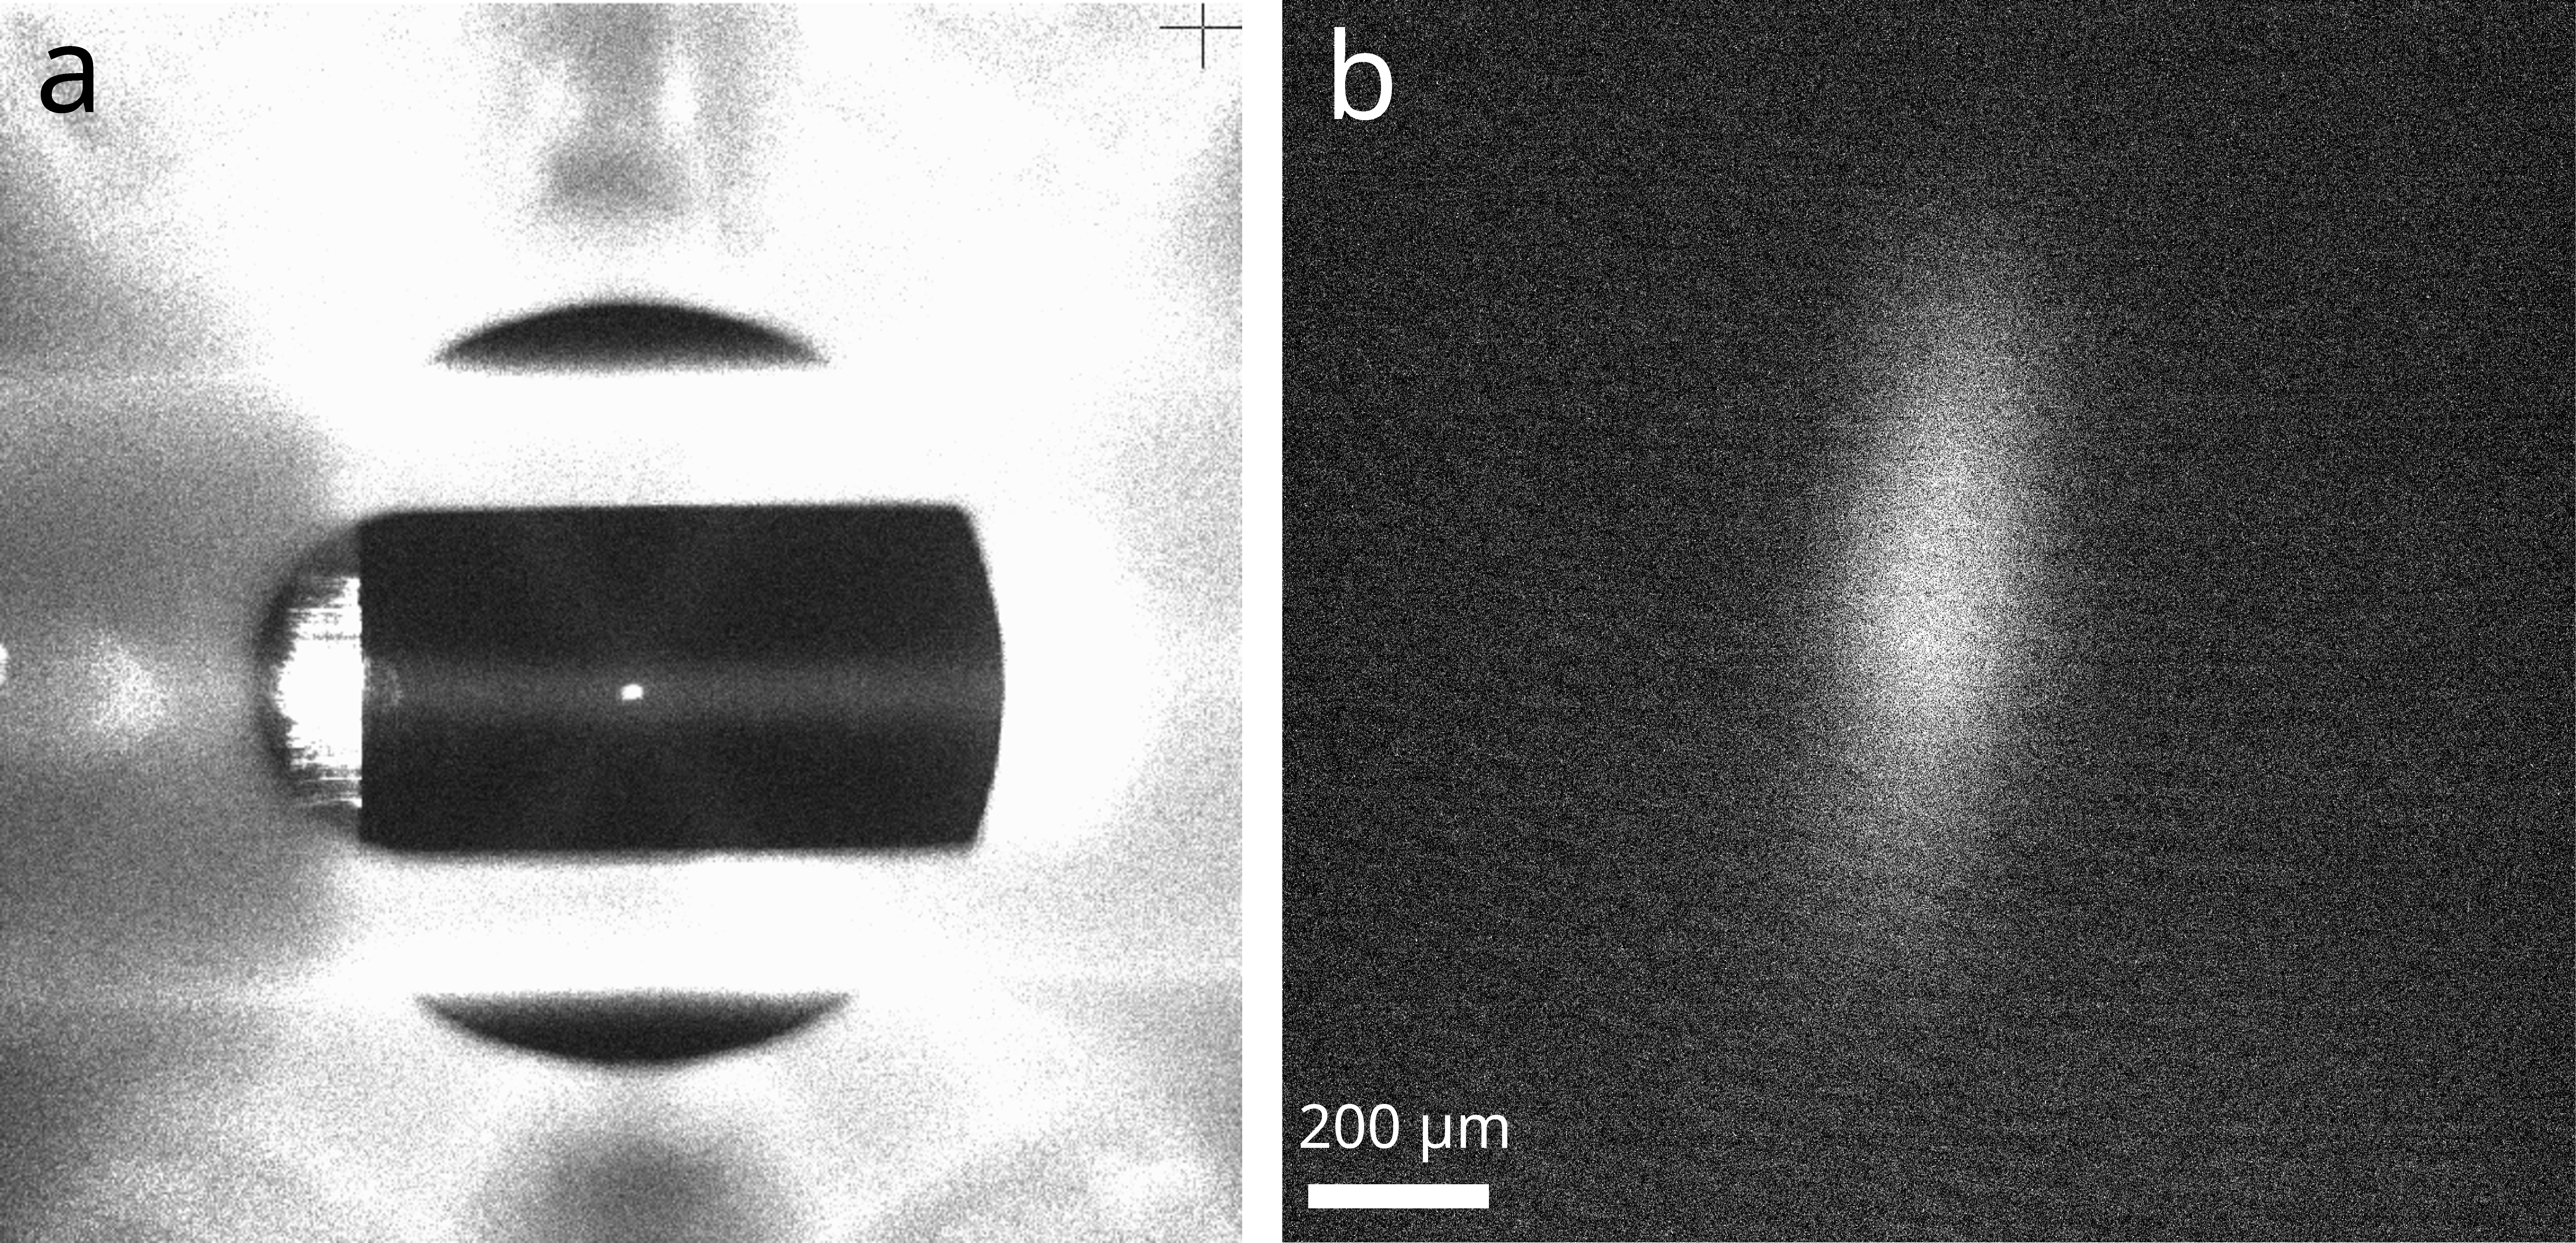
\includegraphics[width=0.9\textwidth]{Images/large_mot_and_thorcam_mot.pdf}
    \caption{(a) A bright MOT captured with Andor Luca, and (b) a more typical MOT 
    as imaged through a custom 0.4 NA objective onto a 
    CS165MU ThorCam.}
    \label{fig:large_mot_and_thorcam_mot}
\end{figure}
An example of a particularly bright MOT is shown in Fig. (\ref{fig:large_mot_and_thorcam_mot}), with a more typical MOT imaged through the bottom objective and 200 mm lens onto a ThorCam CS165MU. The width is about $180~\mu$m in one direction and around twice this in the other. Early measurements of the MOT temperature were done using the time of flight (ToF) technique and the Luca camera imaging through the top window with a zoom lens, giving temperatures around 100 $\mu$K for each axis. However, typically the MOT corresponding to good atom loading is too weak to do ToF imaging with the top camera, and the bottom imaging system has too small a field of view.

\subsection{Fiber AOMs and cooling light power stabilization}\label{sec:fiber_AOM_power_stabilization}

Making sure that the MOT position does not drift over time is crucial for reliable atom loading, especially with a small MOT. One source of instability comes from standing waves between pairs of MOT beams which shift as the phase of the laser varies, causing the MOT to move around. We mitigate this effect by using one fiber AOM for each MOT beam to impart a relative frequency shift of $\sim 10$kHz between any given pair of beams. It can be shown that for $780$ nm light, this corresponds to 5000 intensity waves (with $\lambda=390$ nm) passing through the MOT in a 0.5 s loading period. 

A second source of instability comes from power imbalanced between the pairs of MOT beams, which can also cause variations in MOT temperature. To mitigate this, we employ a DC feedback loop in which the powers of the MOT beams are measured and the corresponding fiber AOMs are used as variable optical attenuators by varying the RF driving power. For the external MOT beams, the power for each beam is measured with a pick-off to an amplified photodiode \cite{Ebert2017thesis} which comes after the polarization optics but precedes the final mirrors before the chamber. For the on-chip beams, the situation is more involved. In order to have a reliable measure of the optical power at the atoms, we measure light which couples from one beam (e.g. 2) into the opposite beam's fiber (e.g. 4), with a free space $30:70$ non-polarizing beamsplitter outside of the chamber, as shown in Fig. (\ref{fig:mot_feedback}). 
\begin{figure}[!ht]
    \centering
    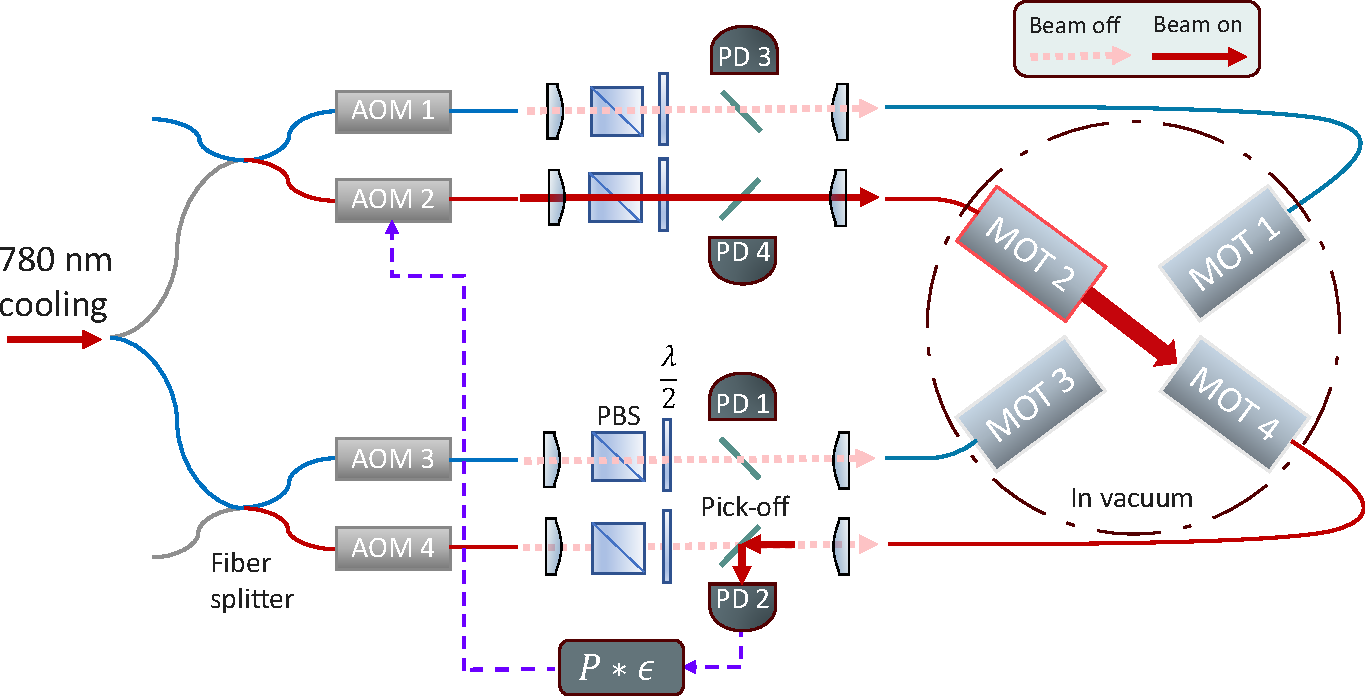
\includegraphics[width=0.9\textwidth]{Images/on_chip_mot_feedback.pdf}
    \caption{Schematic of the DC power stabilization for the on-chip
    MOT beams.}
    \label{fig:mot_feedback}
\end{figure}
This design choice was made for several reasons. Fiber splitter pick-offs could be used before the fibers going to vacuum, but the polarization state after the fiber AOMs drifts, and this is worsened with the addition of a fiber splitter. This means the light after the polarizer in vacuum for a given MOT beam will not correlate with the light measured at the pick-off port of the fiber splitter. Measuring the light after it has come back out of the vacuum  from the opposite fiber allows us to have a reliable proxy for the  light after the polarizer. The reason for doing this in free-space is that we found fiber splitters to have uncorrelated output powers over time, i.e. the splitting ratio varies, such that the pick-off would not be reliable to the degree needed. While having high reliability, our approach some shortcomings. Opposite MOT beams must be turned on one at a time for during the feedback phase, meaning that we can not continuously stabilize the light with a servo loop. This also adds to the amount of time it takes to run feedback, as the beams can not all be done in parallel. Typically, the feedback loop is run every time a MOT is loaded and takes $\sim 100$ ms, limited by averaging time as multiple measurements of the beam powers are recorded with the Sinara Sampler card to adjust the RF to bring the photodiode voltages to defined set points.

\section{Trapping single atoms}
% finding single atom signals. dipole trap beam fixed wrt to 
% on-chip beams, necessity to shim the MOT to the correction position
% we don't need to be able to see the MOT on the SPCM, which is probably 
% explained by the emission of the MOT not coupling well to an SM fiber

\subsection{FORT formed with parabolic mirror}
% The red-detuned dipole trap. scattering rate. Raman scattering. 
% coupling into SM fiber, wonky feedback scheme.

The far-off resonant trap (FORT) used for trapping single atoms is formed by focusing 852 nm light from a DFB laser (Eagleyard) with a 0.6 NA parabolic mirror, resulting in a $\sim0.8~\mu$m waist trap. As described previously, the focal pattern was prealigned to intersect laser cooling beams in the vacuum chamber (Fig. \ref{fig:parabolicfluorescence}).
\begin{figure}[!ht]
    \centering
    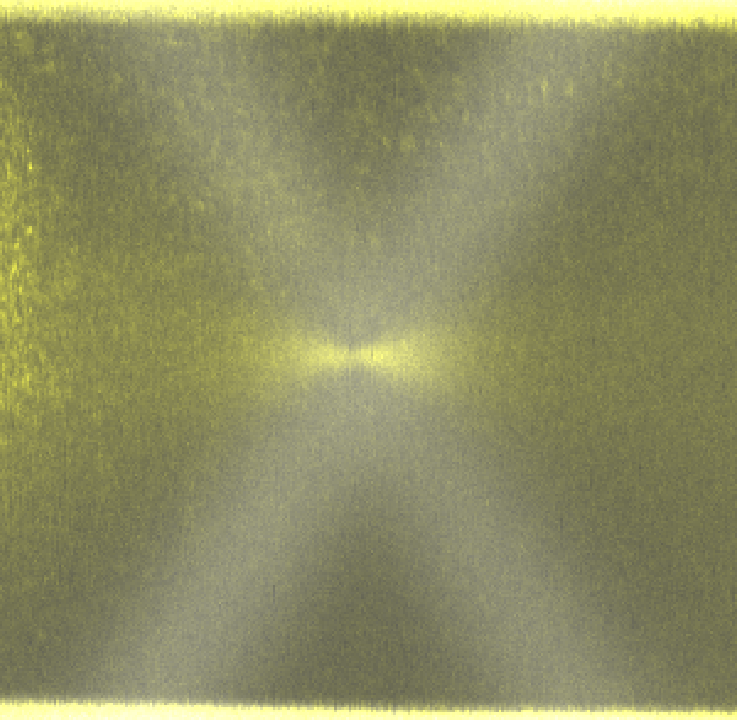
\includegraphics[width=0.5\textwidth]{Images/mirror_fluorescence_and_chip_beams_yellow.pdf}
    \caption{False-color image of the optical path of the FORT (yellow) and the on-chip MOT beams (grey) imaged with fluorescent emission from thermal Rb atoms in the chamber. The image is a combination of two separate images of the MOT beams and FORT path, both with 780 nm light, so that their pixel values could be scaled, clipped, and colored independently for optimal visualization.}
    \label{fig:parabolicfluorescence}
\end{figure}
For consistency in single atom trapping and the experiments to be described later, it is important to stabilize both the power and polarization of the light. Power stability is important to minimize DC drift of the AC Stark shift experienced by the atomic states, for example between $F=1$ and $F=2$ in the ground state during microwave rotations. Maintaining a high degree of linear polarization is typically is necessary for achieving effective polarization gradient cooling (PGC), which can be hindered by the presence of a non-zero vector Stark shift introduced by non-zero ellipticity of the polarization\cite{chin2017polarization}.
% \begin{figure}[!ht]
%     \centering
%     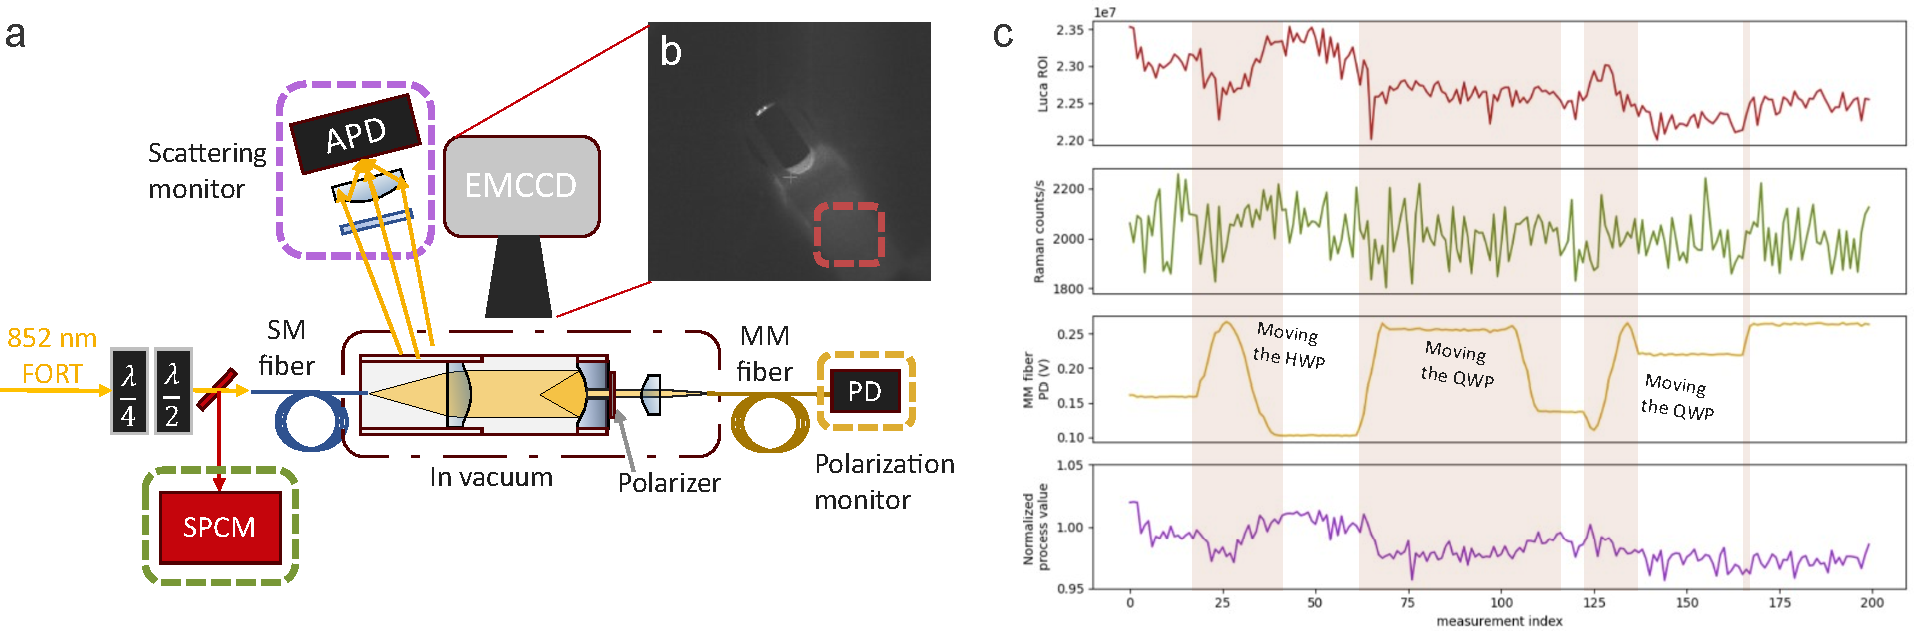
\includegraphics[width=0.9\textwidth]{Images/FORT_feedback.pdf}
%     \caption{Schematic of the polarization for the on-chip
%     of the 852 nm FORT light. DC power stabilization of the FORT is accomplished by measuring light scattered off surfaces in the chamber with an avalanche photodetector (not shown).}
%     \label{fig:fort_feedback}
% \end{figure}

% ?? \textbf{section needs to be reworked}

Because the FORT power is launched into the same SM fiber which carries out 780 nm photons emitted by trapped atoms, it is not possible to simply set a fixed polarization state before the fiber. For this reason, there is a hole bored through the parabolic mirror and a linear polarizer (Skight Optics) mounted behind the mirror, which allows for optimizing the linearity of the polarization by monitoring light coupled out of the vacuum with a MM fiber. The power out of the MM fiber, measured with a photodetector (TTI), can be maximized by adjusting a quarter- and half-waveplate mounted in motorized stages (Thorlabs K10CR1). The polarizer transmission is typically observed to drift by not more than a couple of percent over the course of a day, so for now the polarization is not actively stabilized. We maximize the polarizer transmission "by hand" as needed by controlling the motorized waveplate mounts upstream of the SM fiber.

% The optimization algorithm used and results will be discussed in Sec. \ref{sec:FORTpolarizationOptimization}

\subsection{FORT power stabilization}

\begin{figure}[!ht]
    \centering
    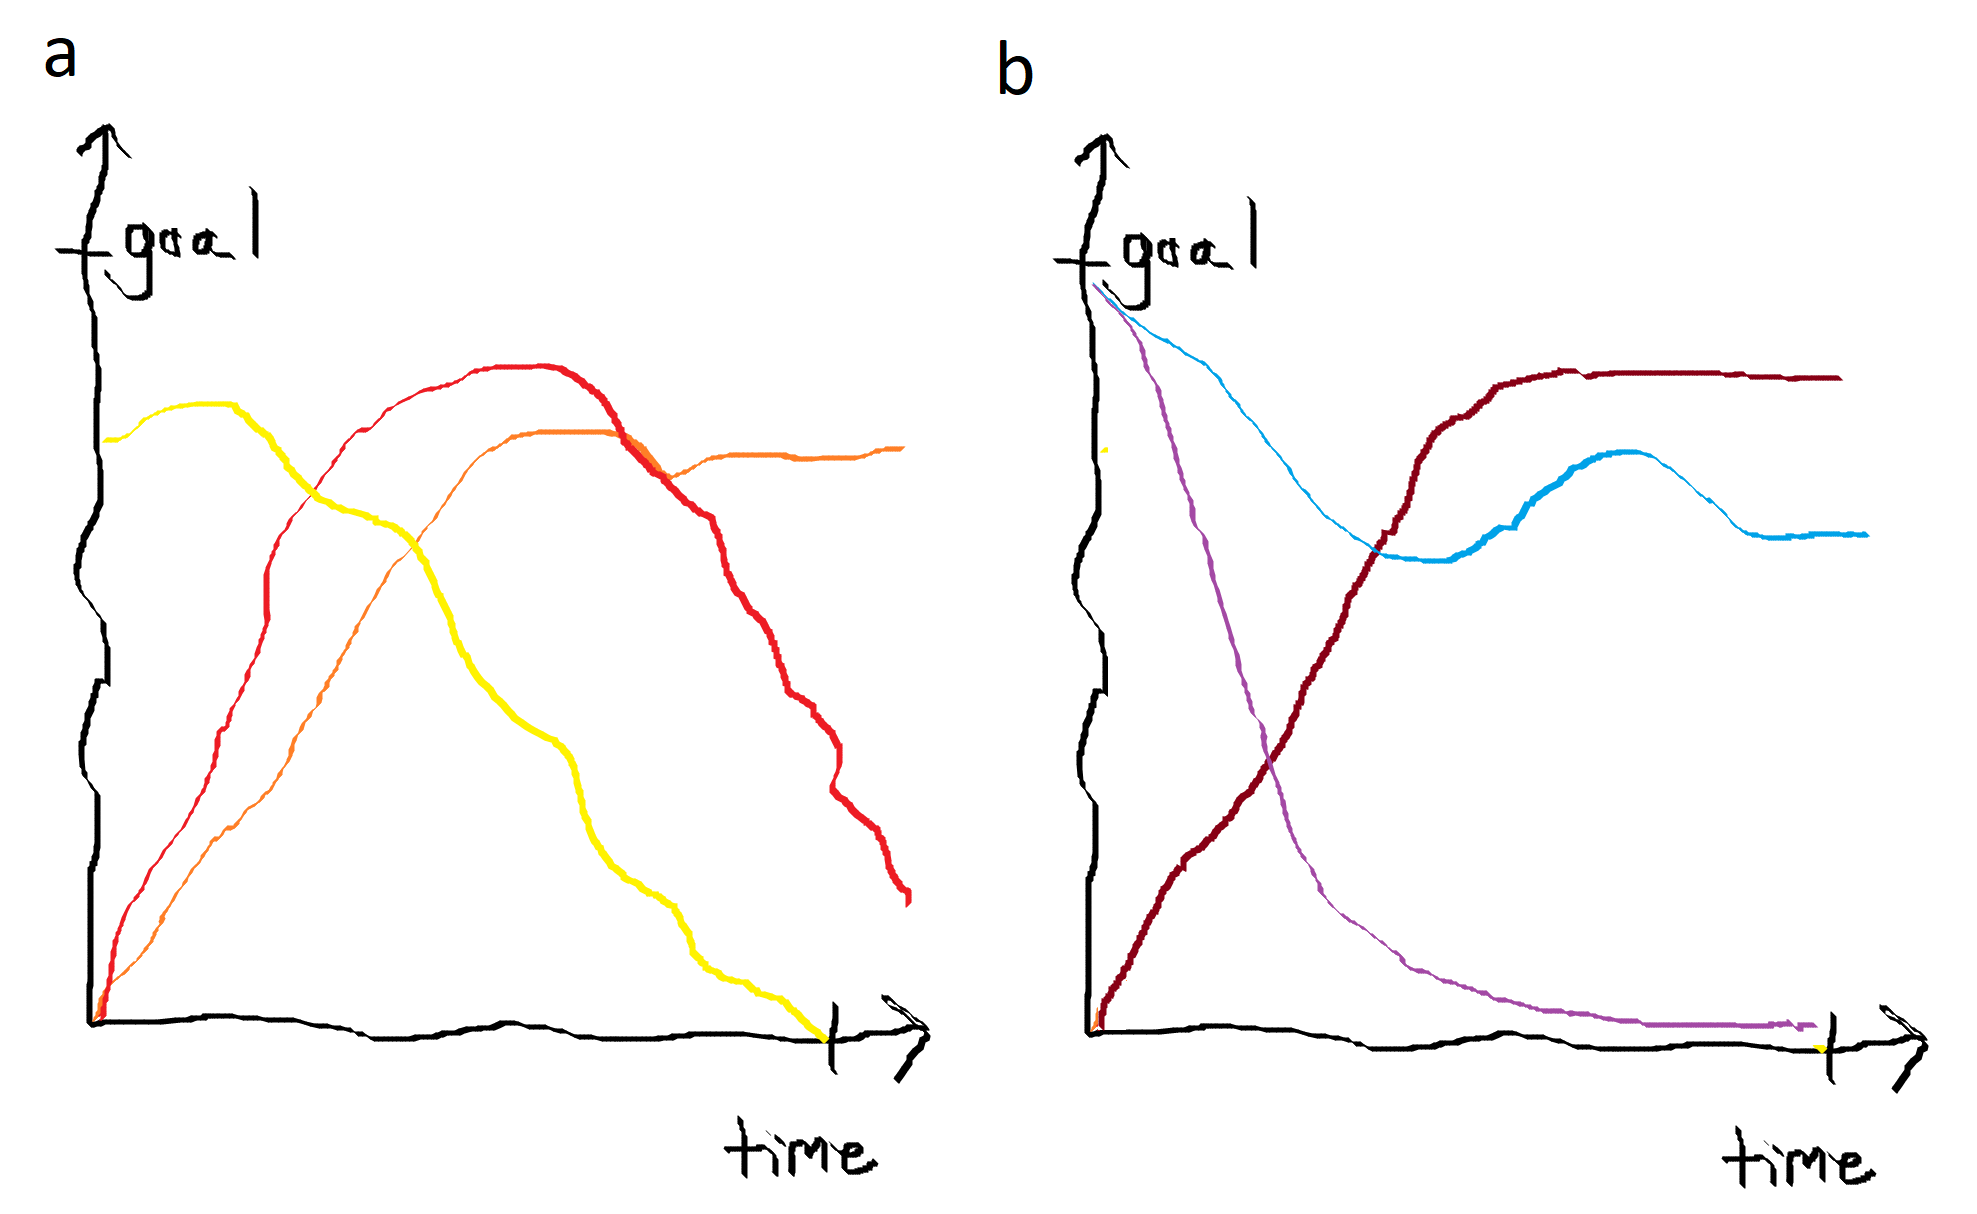
\includegraphics[width=0.9\textwidth]{Images/fig_coming_soon.png}
    \caption{show the measurement where the motorized waveplates were being rotated and the APD did not vary more than a couple of percent.}
    \label{fig:FORTAPDpolarizationtest}
\end{figure}

Stabilizing the optical power of the FORT is done by measuring light scattered off of surfaces in the chamber, primarily the parabolic mirror tube, and feeding back to the FORT AOM as described in Sec. \ref{sec:fiber_AOM_power_stabilization}. A Thorlabs APD430A with an asphere and 780 nm bandpass is mounted outside of the chamber's upper window, positioned for maximum signal from the scattered FORT light. SNR around 50 is typical for the science phase setpoint, and higher than this for the loading setpoint. Because the polarization is not stabilized as often as the power due to the associated cost to the experiment cycle rate, it was necessary to verify that the amount of scattering at the APD did not depend strongly on the polarization of the light. By programmatically rotating the motorized waveplates in the FORT path upstream of the SM fiber, we can maximize and minimize the transmission through the polarizer after the parabolic mirror, and compare with the scattering signal seen by the APD. For redundancy the scattering is also monitored with an EMCCD (Andor Luca). The results of these measurements are shown in Fig. \ref{fig:FORTfeedback}

\begin{figure}[!ht]
    \centering
    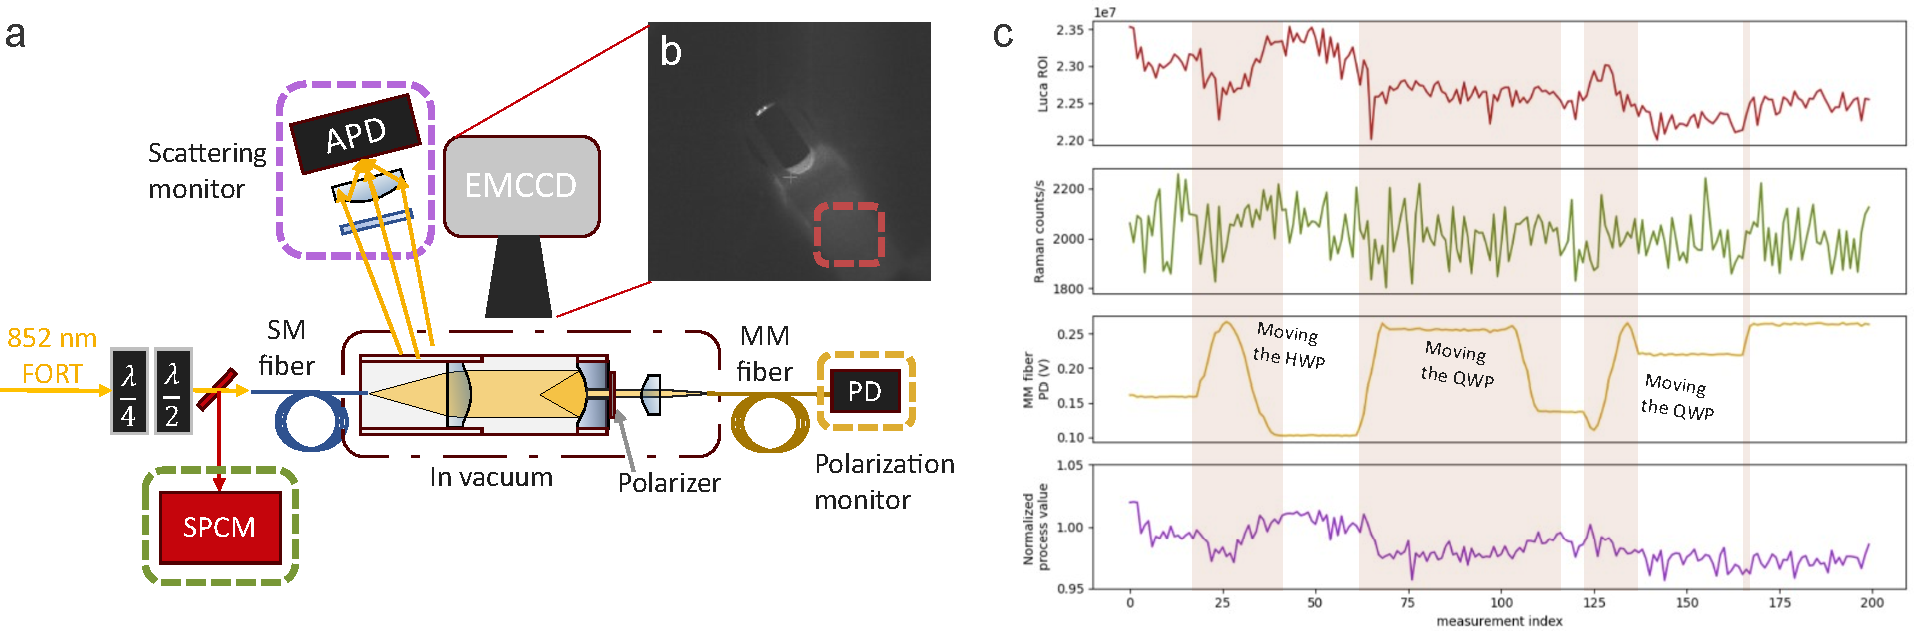
\includegraphics[width=0.9\textwidth]{Images/FORT_feedback.pdf}
    \caption{The feedback scheme for FORT dc intensity stabilization, shown schematically in (a). The inset (b) shows scattering from the FORT light on the Macor mirror tube in the chamber as viewed with an EMCCD. (c) Analysis of the extent to which the scattering monitored with the APD, which is used for dc stabilization of the FORT power, is dependent on polarization. The color of the data corresponds to the detectors outlined in the same color in (a). See text for details.}
    \label{fig:FORTfeedback}
\end{figure}

the FORT light causes enough Raman scattering in the SM fiber at 780 nm, which can not be filtered out of from the light emitted by trapped atoms, and hence shows up during single atom readout

The standard deviation of the Raman light from the SM fiber implies stability of the FORT power at the $1\%$ level, where shot noise can explain 0.7 of this. 

% The astute reader will have noticed that the photodetector's measurement of the FORT power can not distinguish between power and polarization drift, such that the relative rates of polarization and power drifts must be ascertained another way. Fortunately, the FORT light causes enough Raman scattering in the SM fiber at 780 nm, which can not be filtered out of from the light emitted by trapped atoms, and hence shows up during single atom readout, discussed later. When the polarization drifts during experiments, step (1) of the feedback will increase the optical power to bring the measured signal after the polarizer to the setpoint, thus increasing the light at the atoms beyond the intended set point. When this happens, the mean background during atom readout increases, and this can be monitored over many atom readouts in order to extract both the magnitude and rate of polarization drift. See Sec. \ref{sec:single_atom_readout} for relevant data.

% ?? say something about the estimated Raman rate here? maybe just the measured rate

% \subsection{FORT polarization optimization}\label{sec:FORTpolarizationOptimization}

\subsection{Single atom loading in steady-state MOT}
% Scanning the shim fields, monitoring SPCM counts to see atom-loading with
% the MOT and FORT on simultaneously, optimize the number of atoms loaded with
% M-LOOP from Vuletic group.

The first single atom signal in the network experiment was found by manually scanning the magnetic shim coil values and monitoring the counts recorded by a SPCM monitoring the 780 nm light out of the SM fiber. With the FORT turned on with an estimated 1 mK trap depth at the atoms, a sequence of jumps in the typical counts recorded by the SPCM in 10-15 ms exposure times heralds single atoms, shown in Fig. (\ref{fig:atoms_loaded_steady_state}) The hallmark of single atom loading is a bimodal distribution, meaning that there is sub-Poissonian atom loading: the mean number of atoms loaded is less than one, but there are never events with two or more atoms loaded (See Fig. \ref{fig:atom_histogram}).
\begin{figure}[!ht]
    \centering
    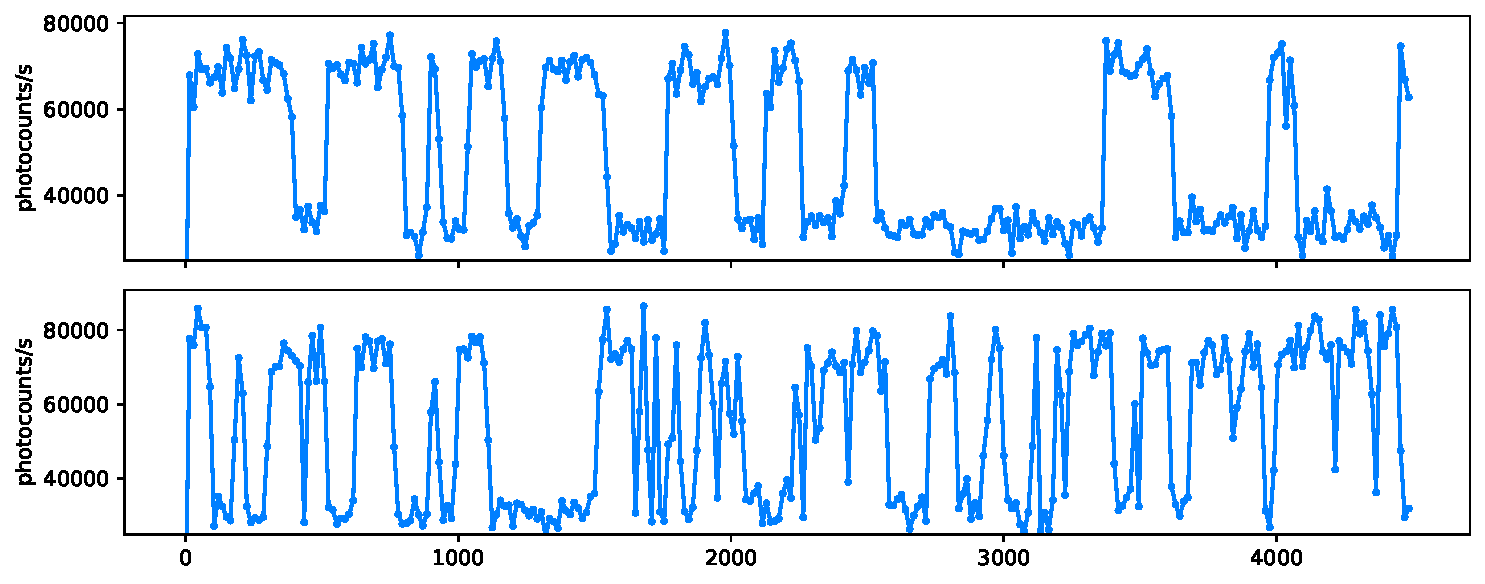
\includegraphics[width=0.9\textwidth]{Images/2024-06-21_atom_loading_with_continuous_MOT_time_series_loading_comparison_aspect0.02.pdf}
    \caption{Photon count rate as atoms enter and leave the FORT with the MOT loaded continuously. The top subplot shows clearly the bimodal nature of the signal, indicating that we load either zero or one atom. The lower subplot shows atoms coming and going more frequently, corresponding to a higher atom loading rate. Note that although the vertical axis is given
    as counts per s, the data collected in the lab is counts, 
    which is then divided by the exposure time for the SPCM here.}
    \label{fig:atoms_loaded_steady_state}
\end{figure}
We initially searched for single atoms by trying to first position the MOT to overlap the focal region of the FORT by watching for an increase in counts from SPCM due to the collected MOT fluorescence. This proved both difficult and unnecessary, as the signal fluorescence signal from the MOT is extremely weak compared to that of a trapped single atom, which we attribute to the multi-mode emission pattern from the MOT not coupling well into an SM fiber. 

The data in \ref{fig:atoms_loaded_steady_state} corresponds to suboptimal loading parameters such that the FORT is likely not overlapped with the most dense part of the MOT, which explains why atoms can remain trapped for 100s of ms. The best single atom loading rate occurs when atoms are kicked out almost immediately after they are trapped, followed by a subsequent loading event.

The single atom loading rate is optimized using by tuning both coils and the power in each MOT beam, while loading the MOT continuously. This is done using an automated optimization routine which minimizes a cost defined as $-1$ times the number of atoms trapped within a 400 ms window. The optimization is done with ARTIQ, using M-LOOP, a machine learning optimization tool developed specifically for cold atom experiments \cite{Wigley2016}. Although single atom experiments in this work are done by loading the FORT over a fixed amount of time (see Sec. \ref{sec:fort_loading}) and then checking for the presence of an atom, the probability of loading an atom in that method reliably corresponds to the loading rate in a steady state MOT. Moreover, this optimization method is at least an order of magnitude faster than optimization by loading the MOT and FORT for fixed times followed by checking for an atom. 

\subsection{Trap depth and vibrational frequencies}

The trap depth and characteristic Gaussian beam waist of the FORT can be measured by doing spectroscopy on the vibrational frequencies of trapped single atoms. Typically, one has an estimate of the trap depth given a measured or calculated beam size, beam power measured before the atoms, and a calculated polarizability of the atomic ground state. For the fiber-couple network node however, our estimate is limited to within a factor of two or so given that we can not directly measure how much 852 nm light couples into the SM fiber. Vibrational spectroscopy of the atom can be performed to allow us to back out these quantities.

A trapped atom in a red-detuned dipole trap can be modeled as a harmonic oscillator in a radially 3D potential well centered on the intensity maximum (see also Sec. \ref{sub:confine}) with radial and axial angular vibrational frequencies related to the trap depth and waist by
\begin{align}\label{eq:trapfreqs}
    \omega_{\rho} &= \frac{2}{w_0}\sqrt{\frac{U_0}{m}} \\
    \omega_z &= \frac{1}{z_R}\sqrt{\frac{2U_0}{m}}
\end{align}
where $w_0$ is the transverse $1/e^2$ intensity waist, $U_0$ is the trap depth, $m$ is the atomic mass, and $z_R=\pi w_0^2/\lambda$ is the Rayleigh range. The trap depth and waist can thus be extracted from spectroscopy of the vibrational frequencies. 

\begin{figure}[!ht]
    \centering
    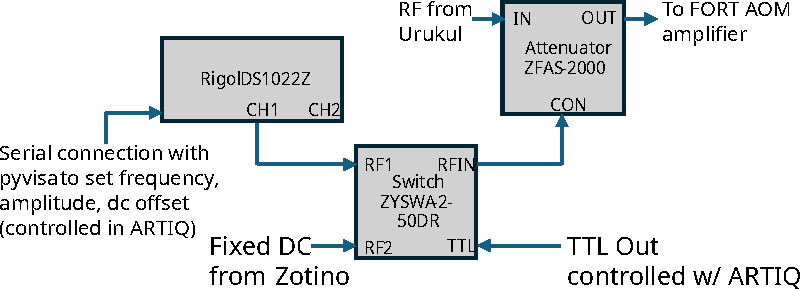
\includegraphics[width=0.9\textwidth]{Images/network_trap_frequency_electronics.pdf}
    \caption{Setup for switching between static and modulated trap for the trap frequency measurement. RF to the FORT AOM is controlled with a voltage controlled attenuator (VCA). The VCA is controlled with a DC voltage for atom loading and readout or modulated with DC + AC from a Rigol function generator between readouts, as determined by a switch.}
    \label{fig:networktrapfrequencyelectronics}
\end{figure}

The trap frequency measurement is done by loading and verifying the presence of an atom in the FORT (see Sec. \ref{sec:singleatomexperiments}), modulating the FORT sinusoidally for a fixed amount of time, and checking whether the atom is retained. Dip in retention will show up when the FORT is modulated at twice the vibrational frequency. The details of the electronics setup for modulating the trap light are shown in Fig. \ref{fig:networktrapfrequencyelectronics} and the measured vibrational spectrum is shown in Fig. \ref{fig:networktrapfrequencies}. We see two radial frequency dips owing to a slightly elliptical transverse trap profile which was first observed during the tapered fiber scans of the mirror focal intensity pattern (see Sec. \ref{sec:mirror}), though we have not come up with a definitive explanation of why the two radial resonances show different depths. 
\begin{figure}[!ht]
    \centering
    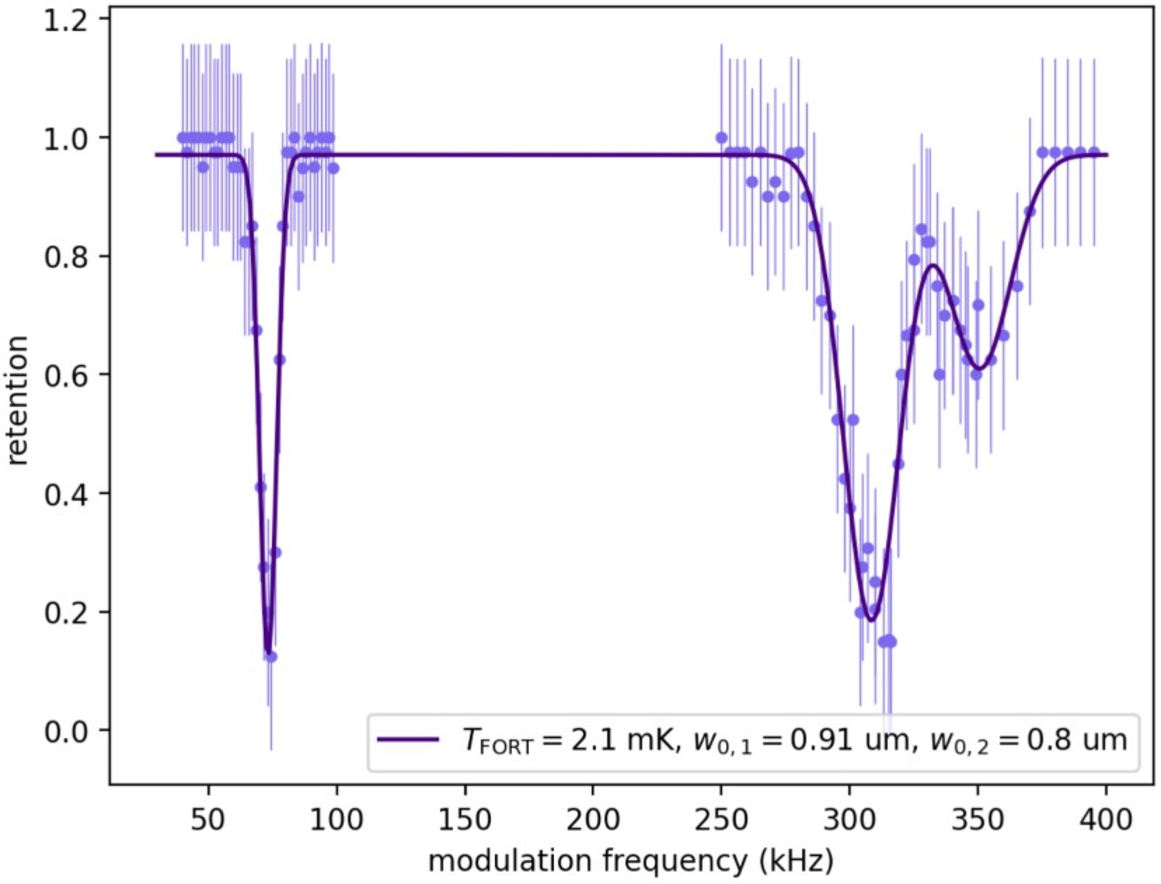
\includegraphics[width=0.9\textwidth]{Images/network_trap_frequencies_20240627.pdf}
    \caption{Vibrational spectroscopy of trapped atoms in the network experiment. The non-degenerate transverse resonances at high frequencies result from slightly different transverse waists in $x$ and $y$. The two axial frequencies at low frequency are not resolved, showing up as a single resonance. The error bars are $1/\sqrt{N}$, with $N$ the number of atoms loaded per data point. The solid line is a fit to a sum of three Gaussians (see text).}
    \label{fig:networktrapfrequencies}
\end{figure}
One possibility is that the modulation of the voltage controlled attenuator (see Fig. \ref{fig:networktrapfrequencyelectronics}) was not as strong for the higher frequency, though that frequency is still well within the 500 kHz control bandwidth. This can easily be checked by viewing the modulation on the FORT light.
    
We extract the trap depth and two beam waists by fitting the data to a sum of three Gaussians and assuming two equations for the transverse beam waist, for a total of three angular frequency relations. The fit frequencies are $(\omega_{\rho,1}, \omega_{\rho,2}, \omega_{z})/2\pi=($154.5 kHz, 175.3 kHz, 36.6 kHz$)$. The waist in the Rayleigh range expression in $\omega_z$ was replaced by the average of the two transverse waists as we do not resolve two axial resonances. Fitting the resulting frequency relations gives a trap depth of $2.1$ mK and transverse waists $w_{0,1}=0.91 ~\mu$m and $w_{0,2}=0.8 ~\mu$m.

\section{Single atom experiments}\label{sec:singleatomexperiments}
% The typical experiment sequence we use.    

\subsection{FORT loading and atom readout}\label{sec:fort_loading}
% Same as continuous MOT loading, but truncated to 500 ms, UV LED pulsed, MOT and FORT loaded, 
% MOT dropped, two readouts with science phase in the middle

% Fluorescence readout, contribution to background from FORT and MOT beams on continuously during readout, histogram, detuning of light, estimation of the power at the atoms.

\begin{figure}[!ht]
    \centering
    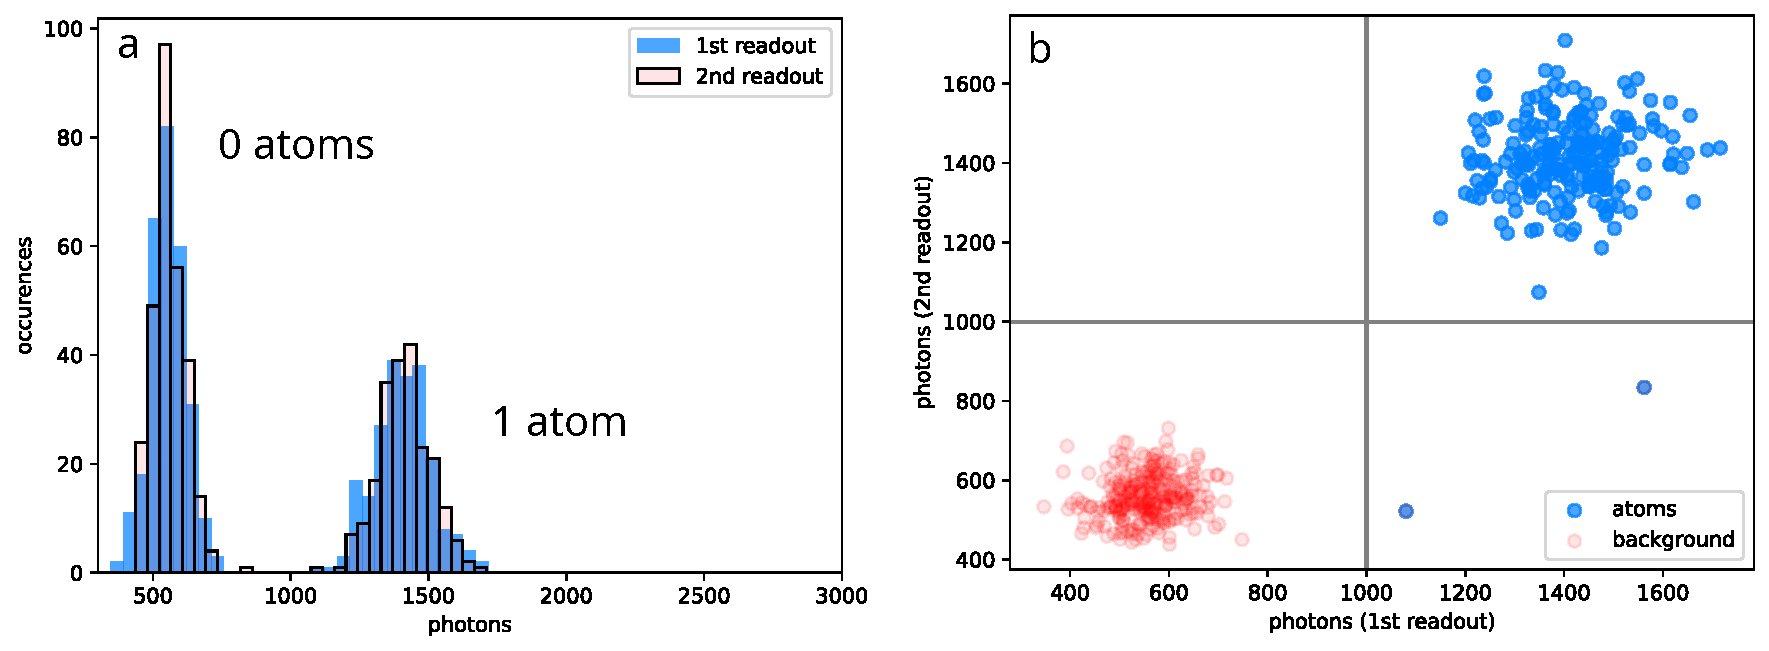
\includegraphics[width=0.9\textwidth]{Images/atom_histogram_and_scatterplot.pdf}
    \caption{Single atom readout data for the two experiment readouts or ``shots". The same data is shown \textbf({a}) as a histogram for each readout and (\textbf{b}) as a scatter plot, for a 14 ms exposure time and 3 ms holding time between shots. There is a clear absence of multi-atom loading events in \textbf{a}, whereas the single atom loading fraction is 44$\%$ \textbf{b} shows that the fraction of atoms detected during the first shot which are also detected in the second, i.e. the retention fraction, is $99\%$.}
    \label{fig:atom_histogram}
\end{figure}

The presence of atoms in the second readout is used as the primary method of answering questions about what we have done to the atom. In specific, every question we want to ask is mapped onto ``with what probability do we expect an atom to be retained?"

\subsection{Limitations to cycle time}
The single atom experiment described above provides the basic framework for most of the experiments described in this thesis. As such, any timing limitations intrinsic to this framework will affect the cycle rate we achieve. The dominant offender is the MOT loading phase, which typically takes 500 ms, depending on the pressure of background atoms in the chamber. Coming in second place is DC feedback to the MOT and FORT power to the atoms, as described in Sec. \ref{sec:fiber_AOM_power_stabilization}, which takes $\sim~100$ ms. Lastly, the two atom readouts take $\sim~10$ ms each. Enhancing cycle time is best achieved by atom reuse, so that we amortize the cost of loading the MOT over many experiments per loading event. This is of high importance for fast entanglement attempt rates (see Sec. \ref{sec:entanglementrate}).

\section{Qubit state preparation}

\subsection{Optical pumping and microwave rotations}
The communication qubit state must be initialized into $\ket{F=1,m_F=0}$ for attempting
atom-photon entanglement generation. For optical pumping into this target state, we drive the $D_1$ transition $F=1 \leftrightarrow F'=1$ with linearly polarized light, fow which the $m_F=0$ to $m_F'=0$ transition is dark. We typically apply a bias field of a few G parallel to the polarization of the light, which coincides with the axis of the parabolic mirror used for photon collection. To avoid worrying about Stark shifts from the FORT, the optical pumping and FORT light are chopped on and off out of phase so that we only address the bare atomic states. 

Optical pumping fidelity is verified by driving the ground state clock transition $\ket{F=1,m_F=0} \leftrightarrow \ket{F=2,m_F=0}$ with microwaves delivered with an external horn, where full population transfer would indicate unity pumping fidelity. A typical microwave Rabi oscillation is shown in \ref{fig:microwave_oscillation}. The observed Rabi oscillation is generally around 30 kHz, which is the correct order of magnitude expected given approximately 3 W microwave power emitted by the horn\cite{kwon2019rydberg}.

%% ?? how much pumping power and pumping time?

\begin{figure}[!ht]
    \centering
    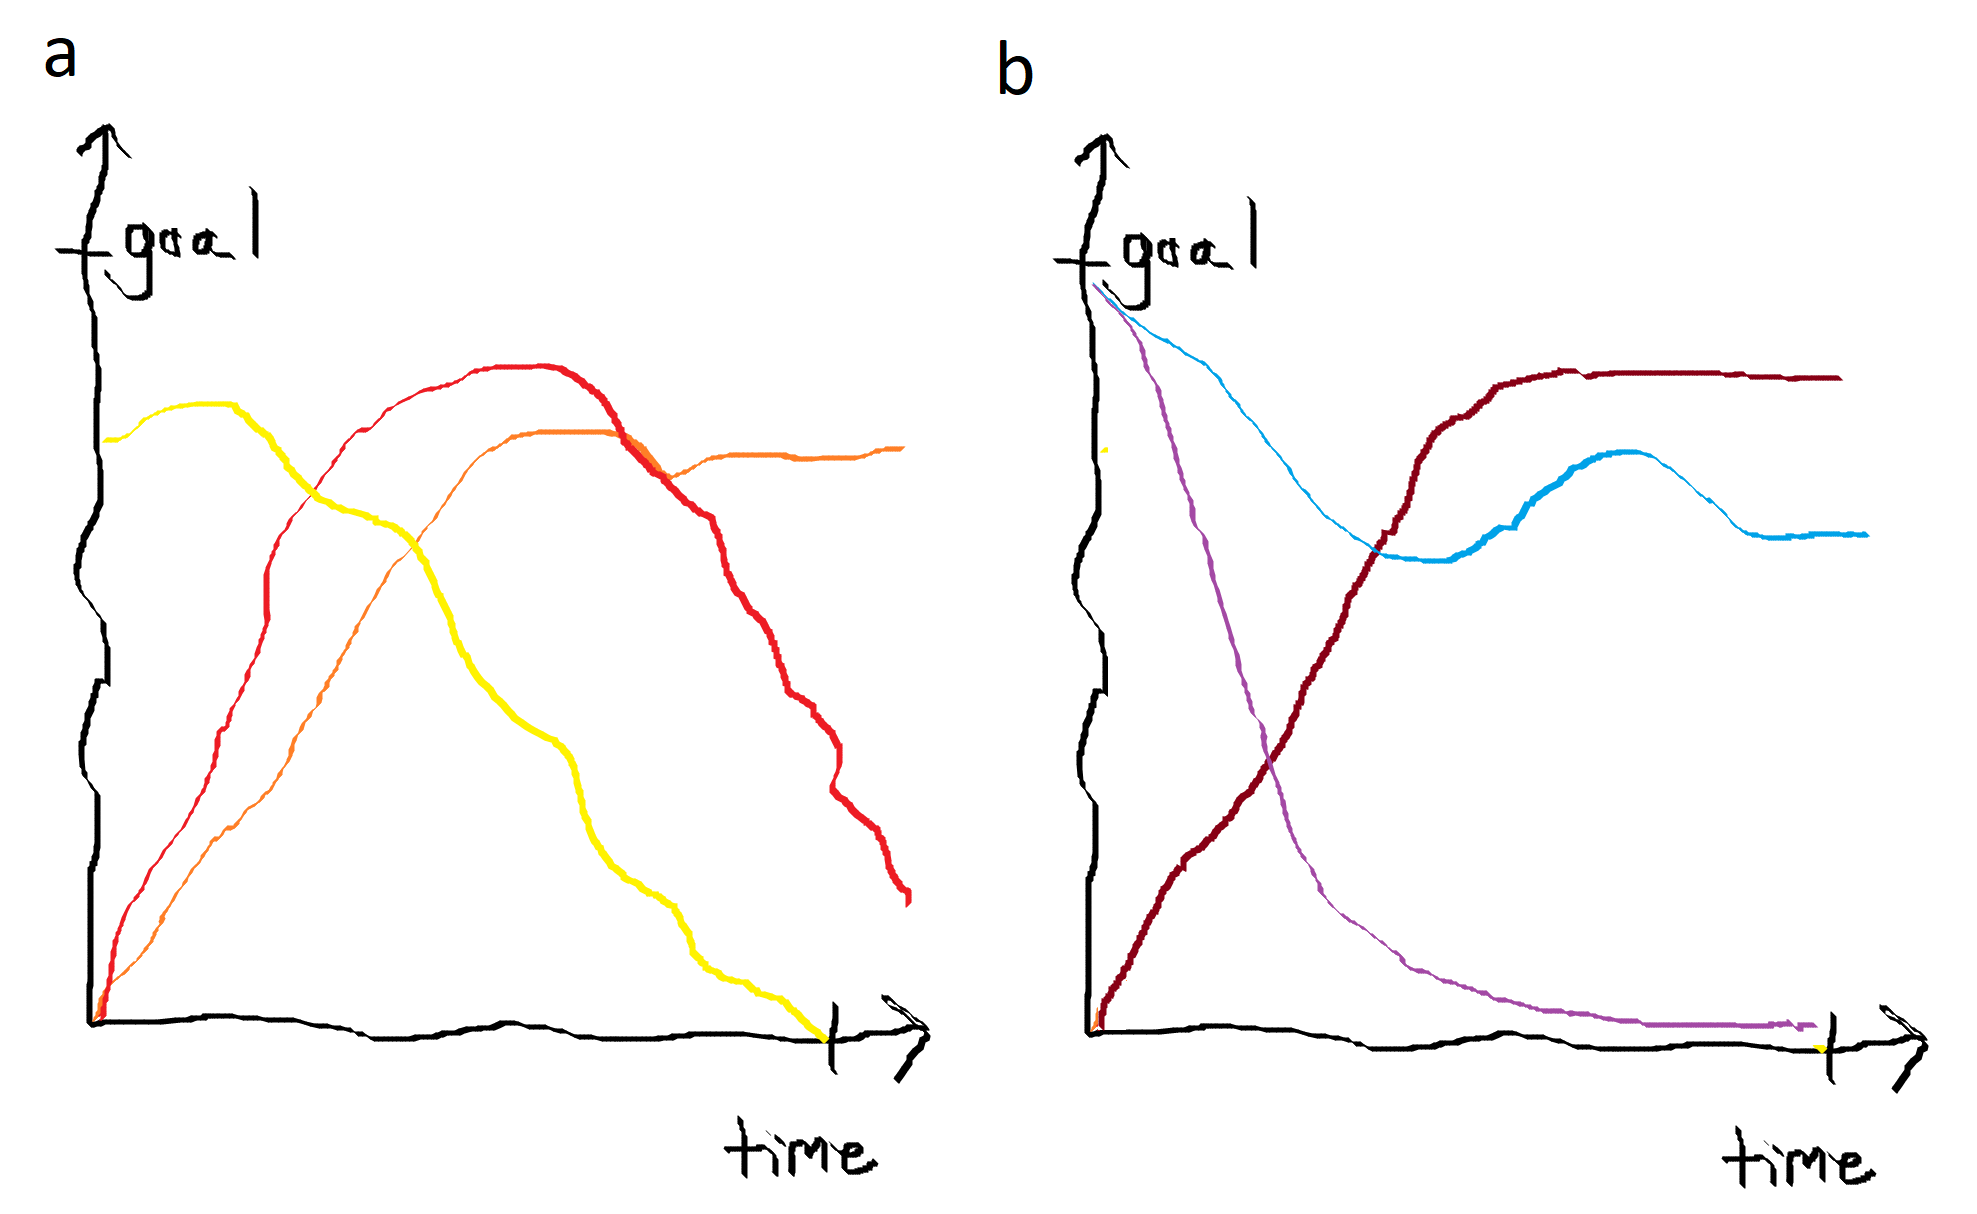
\includegraphics[width=0.9\textwidth]{Images/fig_coming_soon.png}
    \caption{?? put a bad microwave oscillation here}
    \label{fig:microwave_oscillation}
\end{figure}

The microwave system, based on an RF generator (Valon) has been adapted from the one used in \cite{Young2022thesis,kwon2019rydberg}, with minor modifications. The system, along with an RF line for use in the tomography of the atomic state, is shown in Fig. \ref{fig:microwave_system}.

\begin{figure}[!ht]
    \centering
    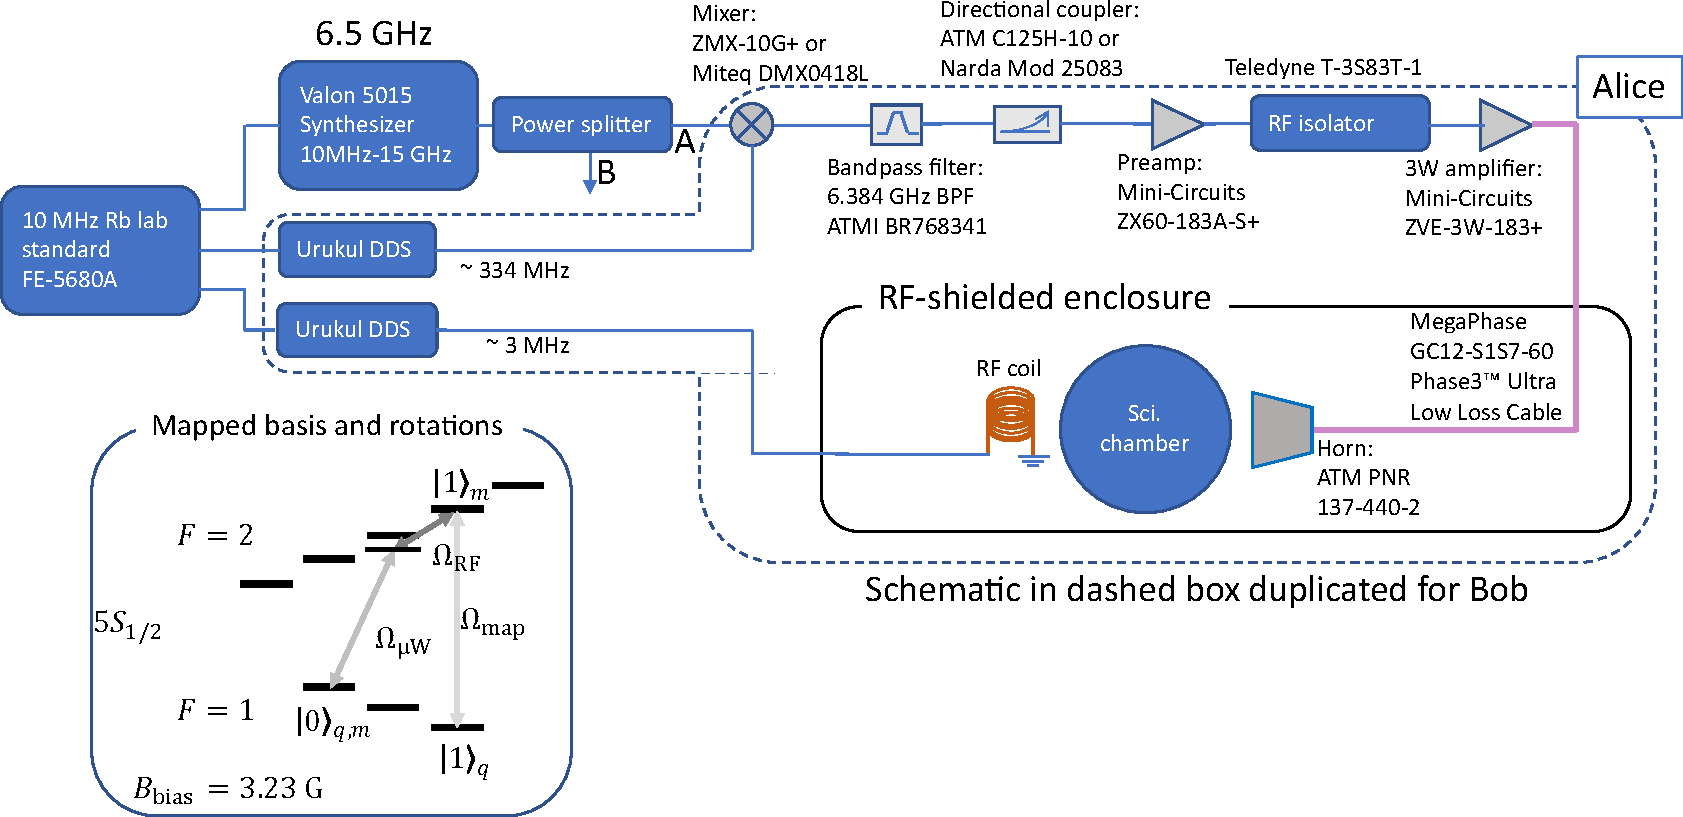
\includegraphics[width=0.9\textwidth]{Images/microwave_system_schematic.pdf}
    \caption{The microwave system used in the quantum network experiment and a (not yet implemented) RF line and coil planned to be used for two-photon rotations in the computational basis used for atom state tomography, as shown in the inset level diagram.}
    \label{fig:microwave_system}
\end{figure}

% \part{Template}\label{part:template}
\chapter{Towards atom-photon entanglement}\label{ch:atomphoton}

% the hierarchy is 
% chapter,section,subsection,etc.

\section{Single photon generation}
The precursor to prepare Bell state between single atoms and emitted photons is the ability to generate a photon from an atom on-demand. With an atom optically pumped into $\ket{5S_{1/2},F=1,m_F=0}$ as described in the previous chapter, $\pi$-polarized 780 nm light incident on the atom can excite it to $\ket{5P_{3/2},F=1,m_F=0}$, where the spontaneous decay is expected to be in a single photon Fock state. Unlike some remote-entanglment protocols which involve weak excitation\cite{cabrillo1999creation}, with an intentionally small probability of exciting the atom, here we employ a $\pi$ pulse so that the population is entirely in the excited state to maximize the per-excitation chance of extracting a photon. 

%% put a level diagram here?

As the lifetime of the $5P_{3/2}$ states is only 27 ns, we would like to excite the atom in less time than this to mitigate decay during the excitation, as this can lead to an effective jitter in the arrival time of photons due to decay during the excitation. Short pulses are broader in frequency and can potentially lead to unwanted excitation. The nearest state that could be excited off-resonantly is $\ket{5P_{3/2},F=2,m_F=0}$, which is nearly 230 MHz away (note that the $\ket{5S_{1/2},F=1,m_F=0} \leftrightarrow {5P_{3/2},F=1,m_F=0}$ transition is electric dipole forbidden because $F$ and $m_F$ do not change). Thus for a pulse of width $\sim$10 ns, we can safely neglect off-resonant driving.

The excitation light, pulsed by an AOM, can be approximated by a Gaussian pulse in order to estimate how much power we need at the atoms for a given pulse width. The requirement to complete full population transfer with a time-varying Rabi frequency is 
\begin{equation}
\int_{t_1}^{t_2} \Omega(t') dt' =\pi
\end{equation}
For $\Omega(t)=\Omega_0 \exp({-\frac{t^2}{2\tau^2}})$, taking $t_1=-\infty$, and $t_2=\infty$ (most of the pule area is contained in a much shorter duration but this allows for a clean analytical result) and we have
\begin{equation} \label{eq:pi}
\begin{split}
\pi & = \Omega_0 \tau \sqrt{2 \pi} \\
 & = \Omega_0 \sqrt{2 \pi} \frac{t_{\textrm{FWHM}}}{2\sqrt{2\ln(2)}} \\
 & = \Omega_0 \sqrt{\pi} \frac{t_{\textrm{FWHM}}}{2\sqrt{\ln(2)}} \\
\end{split}
\end{equation}
which gives
\begin{equation}
    \Omega_0=\frac{2\sqrt{\pi \ln(2)}}{t_{\textrm{FWHM}}}
\end{equation}

% $\pi = \Omega_0 \tau \sqrt{2 \pi}$
% $= \Omega_0 \sqrt{2 \pi} \frac{t_{\textrm{FWHM}}}{2\sqrt{2\ln(2)}}$
% $= \Omega_0 \sqrt{\pi} \frac{t_{\textrm{FWHM}}}{2\sqrt{\ln(2)}}$
% $\Omega_0=\frac{2\sqrt{\pi \ln(2)}}{t_{\textrm{FWHM}}}$

Now we can calculate the power required to have $\Omega_0$ given a beam with a Gaussian spatial intensity pattern with $1/e^2$ waist $w_0$. 
\begin{equation}
    \Omega_0=\frac{dE}{\hbar}
\end{equation}
\begin{equation}
    I_0=\frac{2P_0}{\pi w_0^2}=\frac{1}{2}c \epsilon_0|E|^2
\end{equation}
\begin{equation}
    \Omega_0 =\frac{d}{\hbar}\sqrt{\frac{2I_0}
{c\epsilon_0}}=\frac{d}{\hbar}\sqrt{\frac{4P_0}{c\epsilon_0 \pi w_0^2}}
\end{equation}

Solving for $P_0$ gives
\begin{equation}\label{eq:p0}
\begin{split}
P_0 & = \frac{\hbar^2}{4d^2}\Omega_0^2\pi w_0^2 c \epsilon_0 \\
 & = \frac{\hbar^2}{4d^2} \pi w_0^2 c \epsilon_0 \left(\frac{2\sqrt{\pi \ln(2)}}{t_{\textrm{FWHM}}}\right)^2 \\
 & = \frac{\hbar^2}{d^2} \pi^2 w_0^2 c \epsilon_0\frac{\ln(2)}{t_{\textrm{FWHM}}^2} \\
\end{split}
\end{equation}
resulting in the peak Rabi frequency
\begin{equation}
    \Omega_0=\frac{2\sqrt{\pi \ln(2)}}{t_{\textrm{FWHM}}}.
\end{equation}
It can be shown with dimensional analysis that the units above are in fact power\footnote{Left as an exercise for the younger grad students.}.

The electric dipole matrix element for a transition $F,m_F$ to $F',m_F'$ on the $^{87}\textrm {Rb}$  $D_2$ line is given by
$$d=4.227 e a_0 (-1)^{F'+J+1+I} \sqrt{(2 F'+1)(2 J+1)}\left\{\begin{array}{ccc}
J & J' & 1 \\
F' & F & I
\end{array}\right\}C_{F,m_F;1,-q}^{F',m_F'}$$
with $J=1/2$, $J'=3/2$, and $I=3/2$. The numerical prefactor times $e a0$ is the fine structure reduced matrix element. Note that I use the convention $q = m_F' - m_F$, which opposite of what is used by others, e.g. Steck.
For $F=1, m_F=0$,  $F'=0, m_F'=0$, and linear polarization ($q=0$), we get
$|d|=5.636*10^{-30} ~\textrm{C}\cdot\textrm{m}$.
Now, we can evaluate what peak power we need to drive the $\pi$ rotation. The beam waist from either GRIN lens is about 300 $\mu \textrm{m}$. We can solve for the power with the relations above to get
\begin{equation}
    P_0 = c \epsilon_0 \pi^2 w_0^2 \frac{\hbar^2 \ln(2)}{d^2 t_{\textrm{FWHM}}^2}
\end{equation}
Using $t_{\textrm{FWHM}}=20~ \textrm{ns}$, we find $P_0 = 212~\mu \textrm{W}$.

As a sanity check, we can compare with a square pulse, for which the Rabi frequency needed is simply
\begin{equation}
    \Omega = \frac{\pi}{t}
\end{equation}
where $t$ is the pulse length. From the derivation above, we see \begin{equation}
    \frac{\Omega_{\textrm{square}}}{\Omega_{\textrm{Gaussian}}}=\frac{1}{2}\sqrt{\frac{\pi}{\ln(2)}} \approx 1.06
\end{equation}
The Rabi frequency scales as the square root of the power, so we have
\begin{equation}
\frac{P_{\textrm{square}}}{P_{\textrm{Gaussian}}} \approx 1.12
\end{equation}
Evidently, one needs about $10\%$ more power to excite with a Gaussian pulse of the same nominal temporal length.


% \part{Experiment}\label{part:experiment}
\chapter{A simple, passive design for large optical trap arrays}\label{ch:array_pra}

% the hierarchy is 
% chapter,section,subsection,etc.


% ****** Start of file apssamp.tex ******
%
%   This file is part of the APS files in the REVTeX 4.2 distribution.
%   Version 4.2a of REVTeX, December 2014
%
%   Copyright (c) 2014 The American Physical Society.
%
%   See the REVTeX 4 README file for restrictions and more information.
%
% TeX'ing this file requires that you have AMS-LaTeX 2.0 installed
% as well as the rest of the prerequisites for REVTeX 4.2
%
% See the REVTeX 4 README file
% It also requires running BibTeX. The commands are as follows:
%
%  1)  latex apssamp.tex
%  2)  bibtex apssamp
%  3)  latex apssamp.tex
%  4)  latex apssamp.tex
%
% \documentclass[%
%  reprint,
% superscriptaddress,
% %groupedaddress,
% %unsortedaddress,
% %runinaddress,
% %frontmatterverbose, 
% %preprint,
% %preprintnumbers,
% %nofootinbib,
% %nobibnotes,
% %bibnotes,
%  amsmath,amssymb,
%  aps,
%  pra,
% %prb,
% %rmp,
% %prstab,
% %prstper,
% %floatfix,
% ]{revtex4-2}

% \usepackage{dcolumn}% Align table columns on decimal point
% \usepackage{bm}% bold math
% \usepackage{float} % for precise figure placement
%\usepackage{mathtools} % for equation alignment
%\usepackage{color}  % for coloring edit command
%\usepackage{hyperref}% add hypertext capabilities
%\usepackage[mathlines]{lineno}% Enable numbering of text and display math
%\linenumbers\relax % Commence numbering lines

%\usepackage[showframe,%Uncomment any one of the following lines to test 
%%scale=0.7, marginratio={1:1, 2:3}, ignoreall,% default settings
%%text={7in,10in},centering,
%%margin=1.5in,
%%total={6.5in,8.75in}, top=1.2in, left=0.9in, includefoot,
%%height=10in,a5paper,hmargin={3cm,0.8in},
%]{geometry}
 
% Mark's template for an initial-tagged comment cmd
% \newcommand{\ColorComment}[3]{%
% 	{\colorbox{#1}{\color{white}   \textsf{\textbf{#2}}} \textcolor{#1}{#3}}}
%  Colorful box, initials, phrase 

% \definecolor{mscolor}{rgb}{0,0.5,0.5}\newcommand{\ms}[1]{\ColorComment{mscolor}{ms}{#1}}

% \definecolor{tgcolor}{rgb}{0.5,0,0.5}\newcommand{\tg}[1]{\ColorComment{tgcolor}{tg}{#1}}

% Preston's commands - Optica doesn't want me to use these
% \newcommand{\um}{~\mathrm{ \mu m}}
% \newcommand{\figref}{Fig. \ref}{}
% \definecolor{phcolor}{rgb}{0.5,0,0.5}\newcommand{\PH}[1]{\ColorComment{phcolor}{PH}{#1}}
% \begin{document}

% indexing codes-- do these go in the manuscript somewhere?
% styleguide says i choose four.
% 32.80.Pj Optical cooling of atoms; trapping
% 33.80.P Optical cooling and trapping of atoms and molecules
% 32. Atomic spectra and interactions with photons
% 42. Optics

% \preprint{APS/123-QED}

% \title{A simple, passive design for large optical trap arrays for single atoms}

% \title{A simple, passive design for large optical trap arrays for single atoms}

% \author{P. Huft}%
%  \email{huft@wisc.edu}
% \affiliation{%
% Department of Physics, University of Wisconsin-Madison, 
%  1150 University Avenue,
%  Madison, WI 53706
% }
% \author{Y. Song}
% \affiliation{%
% Department of Physics, University of Wisconsin-Madison, 
%  1150 University Avenue, 
%  Madison, WI 53706
% }

% \author{T. M. Graham}
% \affiliation{%
% Department of Physics, University of Wisconsin-Madison, 
%  1150 University Avenue, 
%  Madison, WI 53706
% }

% \author{K. Jooya}
% \affiliation{%
% Department of Physics, University of Wisconsin-Madison, 
%  1150 University Avenue, 
%  Madison, WI 53706
% }

% \author{S. Deshpande}
% \author{C. Fang}
% \author{M. Kats}
% \affiliation{%
% Department of Electrical and Computer Engineering, University of Wisconsin-Madison, 
%  1415 Engineering Drive, 
%  Madison, WI 53706
% }

% \author{M. Saffman}
% \affiliation{%
% Department of Physics, University of Wisconsin-Madison, 
%  1150 University Avenue, 
%  Madison, WI 53706
% }
% \affiliation{ColdQuanta, Inc.,  111 N. Fairchild St., Madison, WI 53703}

% \date{\today}% It is always \today, today,
%              %  but any date may be explicitly specified

% \begin{abstract}
% We present an approach for trapping cold atoms in a 2D optical trap array
% generated with a novel $4f$ filtering scheme and custom transmission
% mask without any active device. The approach can be used to
% generate arrays of bright or dark traps, or both simultaneously with a single wavelength for forming two-species traps. We demonstrate the design by creating a 2D array of 1225 dark trap sites, where single Cs atoms are loaded into regions of near-zero intensity in an approximately
% Gaussian profile trap. Moreover, we demonstrate a simple solution
% to the problem of out-of-focus trapped atoms, which occurs due to
% the Talbot effect in periodic optical lattices. Using a high power yet low cost  spectrally and spatially broadband
% laser, out-of-focus interference is mitigated, leading to near perfect
% removal of Talbot plane traps.
% \end{abstract}

% \maketitle

This chapter is a reproduction of \cite{PHuft2022}, with the addition of some data not shown in the paper, including the trap vibrational frequency spectroscopy data and image of atoms in a trap array formed with coherent light. Moreover, two new subsections have been included: one outlining a measurement of the vacuum chamber pressure using the MOT loading rate is included, and one showing experimental results for a prototypical dual species trap array. The appendices of the original publication have been recast as subsections. Since the publication of this work, there have been several other nice demonstrations of large atom arrays, which we would be remiss not to cite here \cite{manetsch2024,Pause2024,gyger2024continuous}. The field has thus far voted with their actions largely in favor of forming trap arrays with active optics rather than passive solutions. This is perhaps not surprising given the flexibility afforded by these approaches. Indeed, for some architectures, reconfigurable traps are a necessity rather than a mere convenience, in particular for transport or zone-based quantum computing\cite{Bluvstein2022,li2024high}.

% \section{Abstract}

% We present an approach for trapping cold atoms in a 2D optical trap array
% generated with a novel $4f$ filtering scheme and custom transmission
% mask without any active device. The approach can be used to
% generate arrays of bright or dark traps, or both simultaneously with a single wavelength for forming two-species traps. We demonstrate the design by creating a 2D array of 1225 dark trap sites, where single Cs atoms are loaded into regions of near-zero intensity in an approximately
% Gaussian profile trap. Moreover, we demonstrate a simple solution
% to the problem of out-of-focus trapped atoms, which occurs due to
% the Talbot effect in periodic optical lattices. Using a high power yet low cost  spectrally and spatially broadband
% laser, out-of-focus interference is mitigated, leading to near perfect removal of Talbot plane traps.

\section{Introduction}
Optical trap arrays are a key ingredient in neutral atom based quantum technologies, including quantum computing, quantum simulation, and quantum sensing, due to their stability and versatility \cite{Kaufman2021,Morgado2021}. This is the result of advances over the past two decades in creating low-entropy arrays of single atoms, which have made optical trap arrays ubiquitous in quantum science. However, the optical setups for creating these traps are often complicated, space-consuming, and expensive, requiring active electro-optical devices such as liquid crystal spatial light modulators (SLMs)\cite{DKim2019}, acousto-optic deflectors (AODs)\cite{Graham2022}, and digital micromirror devices (DMDs)\cite{YWang2020}. In response to this experimental overhead, we propose a simple method of creating optical trap arrays using only passive components, consisting of a mask with a custom transmission pattern and a $4f$ imaging setup with a Fourier plane iris for spatial filtering.

Two major advantages exist for optical traps created with passive rather than active components: 1) passive components are free from noise associated with active devices, such as intensity flicker which can lead to short trap lifetimes \cite{Stuart2018}, and 2) they have the capability to handle high optical powers which enables scaling to very large trap arrays. The approach we demonstrate uses a passive amplitude mask, which has some advantages over a passive hologram. Specifically, an amplitude mask can be used with a broad range of wavelengths, and can also be used with incoherent light, which we show can be used for mitigating the Talbot effect for periodic trap arrays. We show how the same basic working principle can be used to create both bright and dark traps, where atoms are trapped in regions of high and low intensity, respectively. Moreover, this approach can be used to create a dual-grid of both dark and bright traps for confining two different atomic species\cite{Singh2022} using only one passive optical mask and a single trapping wavelength. We show as a proof of principle the creation of a two-dimensional 1225-site  array which is used for trapping single Cs atoms in blue-detuned dark traps. Several other recent experiments have demonstrated large atom arrays \cite{YWang2020,Scholl2021,Ebadi2021}. However, all of these relied on active devices. A microlens array can be used to create an array of red-detuned bright traps without requiring any active devices\cite{deMello2019}, but cannot be easily extended to the dark and bright-dark arrays described here.  

The paper is organized as follows. In sec. \ref{sec:theory}, the working principle is discussed for creating an array of bright red-detuned traps, dark blue-detuned traps, or a combination of the two. In sec. \ref{sec:exp}, we discuss an experimental demonstration of trapping single Cs atoms in a dark trap array, and show that the Talbot effect can be mitigated by using incoherent trap light. 

\section{Working Principle} \label{sec:theory}

\subsection{Bright Trap Array}
Here we discuss the case of creating an array of bright optical dipole traps, in which atoms are trapped in regions of maximum intensity for light which is far-detuned red of an atomic transition. Consider a plane wave, incident on an opaque mask with a fully transmitting aperture of radius $a$ (Fig. \ref{fig:working_principle}). If the illuminated mask is placed in the front focal plane of a lens $f_1$, the field in the back focal plane is the familiar Airy disk, which is the Fourier transform of the top hat profile of the field just after the mask. Because the Fourier plane field gives the spatial frequency spectrum of the front focal plane field, we can reason that filtering out higher spatial frequencies from the Airy disk will have the effect of creating a low-passed top hat beam after a second lens transformation.  
\begin{figure*}
    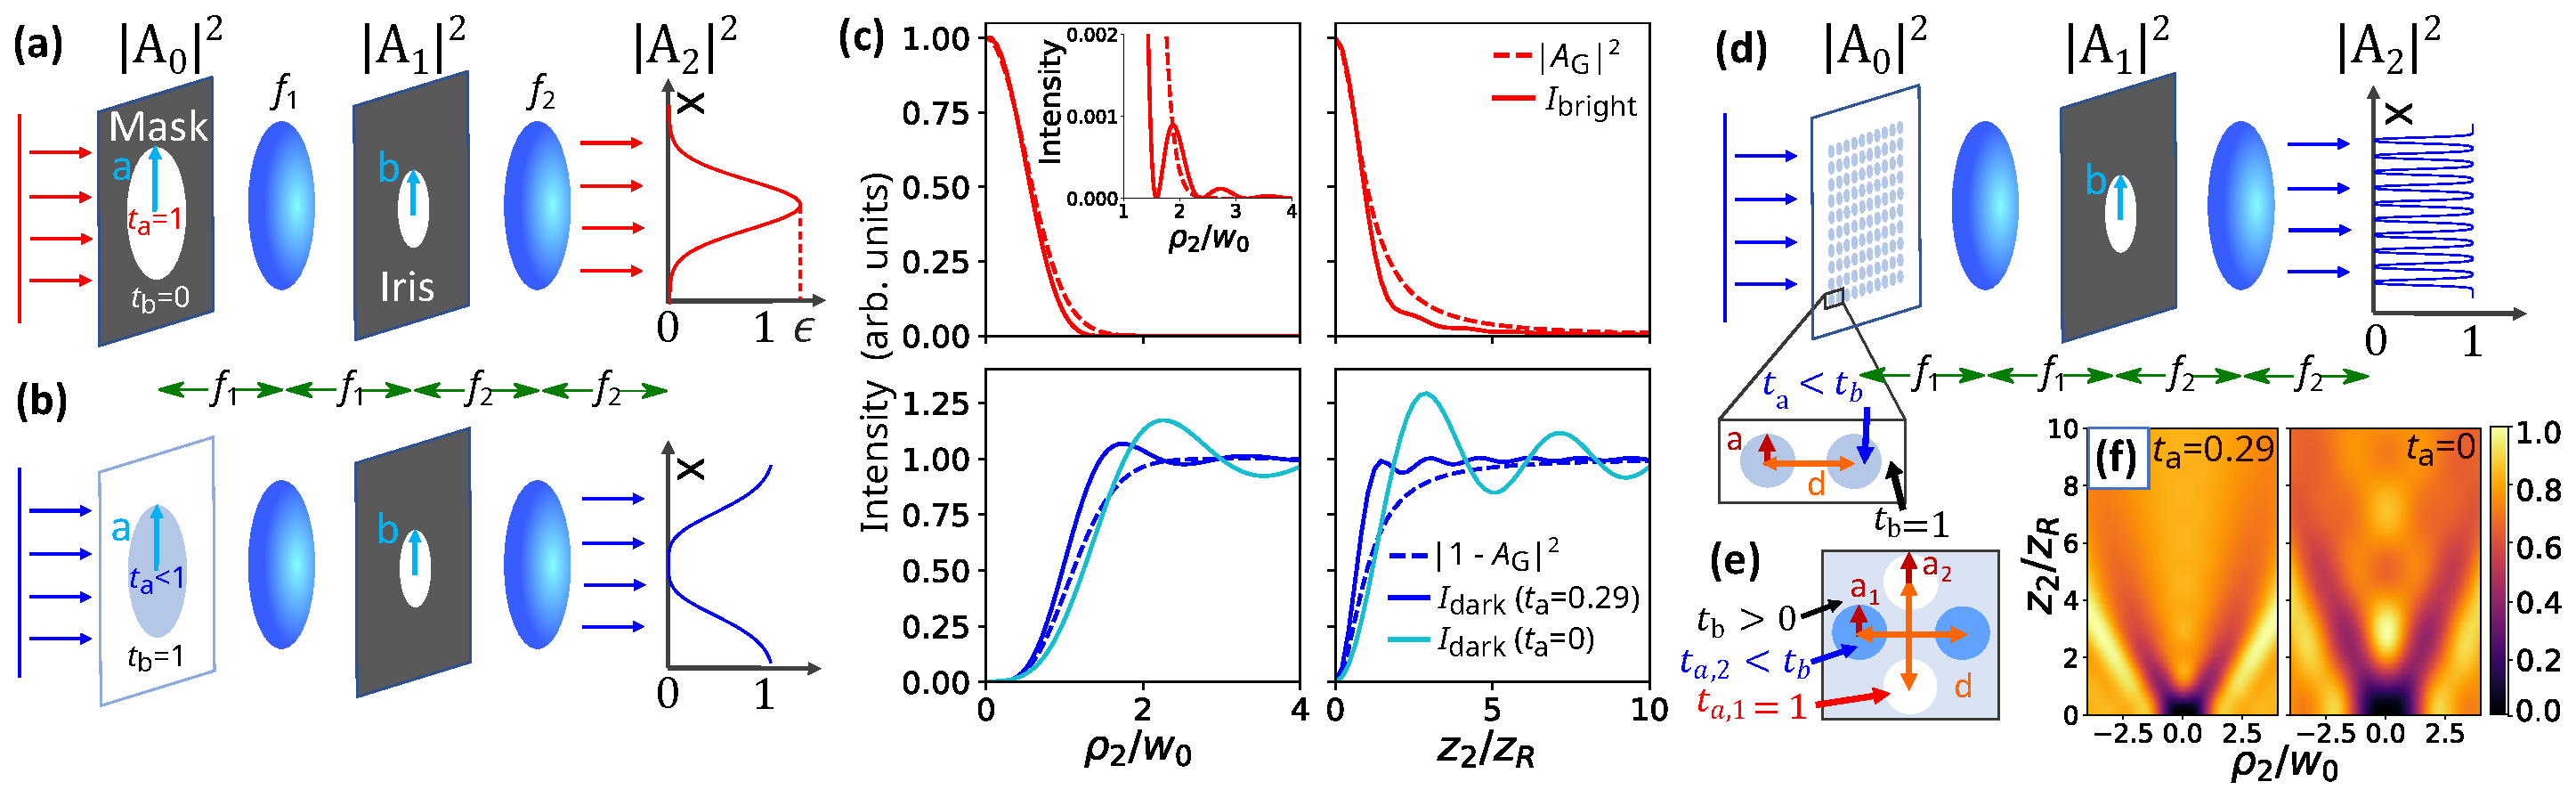
\includegraphics[width=\textwidth]{Images/figure1.eps}
    \caption{Working principle for creating approximately Gaussian (aG) field profiles using a $4f$ filtering scheme. \textbf{(a)} The design for producing a bright trap from an approximately Gaussian beam. An input plane wave is apertured by an opaque mask with a transmitting hole of radius $a$ to create a top-hat profile. A spatial filter or iris of radius $b$ in the Fourier plane transmits only the central lobe of the Airy disk. After transforming through lens $f_2$, the output field, $A_2$, is an approximately Gaussian (aG) beam. \textbf{(b)} Dark traps can be produced with a mask which is fully transmitting with a partially transmitting aperture, for which the output is the aG field subtracted from a plane wave. \textbf{(c)} Intensity profiles of bright (red) and dark (blue) traps based on aG beams (solid lines) compared to their Gaussian (dashed lines) counterparts plotted in terms of the Gaussian waist $w_0$ and Rayleigh range $z_R=\pi w_0^2/\lambda$ for the Gaussian bright trap. The bright traps are normalized to their respective peak focal plane intensities and the dark traps are normalized to the asymptotic intensity at large $\rho_2,z_2$. The inset shows a zoomed in view of the higher order deviation between the aG and Gaussian beam. The axial ($\rho_2=0$) and radial ($z_2=0$) profiles for the bright and dark aG trap are computed numerically using Fresnel diffraction theory. The pairs of dark and light solid blue curves have $t_a=0.287$, $t_a=0$, respectively. For all aG beam curves,  $a=100 ~\mathrm{ \mu m}$ and $b=f_1 x_1^{(1)}/a k$, except for the light blue ($t_a=0$) curve, which has $b=f_1 x_1^{(0)}/a k$. The other simulation parameters are $\lambda=825$ nm, and $w_0=0.974(f_2/f_1)a$ and $w_0=0.943(f_2/f_1)a$ for the bright and dark Gaussian beams, respectively. \textbf{(d)} Extension of the $4f$ filtering scheme to produce a 2D grid of dark traps, using a mask with a grid of apertures with spatial period $d$. \textbf{(e)} A dual grid of bright and dark traps with a single wavelength can be made with a mask which has finite background transmission $t_b$ populated a grid of fully transmitting ($t_{a,1}=1$) apertures and a dual grid of apertures with transmission $t_{a,2} < t_b$. \textbf{(f)} Dark trap profiles in the $\rho z$ plane corresponding to the blue and light blue solid curves in (c), normalized to their respective peak intensities.}
    \label{fig:working_principle}
\end{figure*}
Placing an iris of radius $b$ in the Fourier plane to filter the Airy disk and transform through lens $f_2$, the output field in the back focal plane found from Fresnel diffraction theory is 
\begin{equation}
A_{2}\left(\rho_{2}\right)=-A_{0} \frac{a k}{f_{2}} \int_{0}^{b} d \rho_{1} J_{0}\left(\frac{\rho_{2} k}{f_{2}} \rho_{1}\right) J_{1}\left(\frac{a k}{f_{1}} \rho_{1}\right).
\label{eq:a2_field}
\end{equation}
 The finite Bessel integral above can be expressed as a power series in $b$ using 
\begin{eqnarray}
     &&\int_{0}^{b} d z J_{0}(c z) J_{1}(d z) \nonumber\\
     &=& 
  \sum_{j=0}^{\infty} \frac{(-1)^{j}}{j !(j+1) !(2 j+2)} \nonumber\\
  &\times&  { }_{2} F_{1}\left(-j,-1-j ; 1 ; c^{2} / d^{2}\right) b^{2+2 j}(d / 2)^{1+2 j}\nonumber
\end{eqnarray}
where $_2F_1$ is the hypergeometric function \cite{pochernyaev1995}. Taking $f_1 = f_2 = f$ and setting $b=\frac{f}{a k} x_1^{(1)}$, where $x_1^{(1)}=3.8317$ is the first zero of $J_1$, allows further simplification. This choice for $b$ corresponds to filtering off the lobes beyond the central bright spot, constituting a power loss of only 16$\%$. With these choices, we can then express the intensity in the output plane $I_2$, normalized to the input intensity $I_0$, as a power series in $\rho_2/a$:
\begin{equation}\label{eq:Iag_radial}
    \frac{I_{2}\left(\rho_{2},z_2=0\right)}{I_{0}}=1.97-4.15\left(\frac{\rho_{2}}{a}\right)^{2}+3.92\left(\frac{\rho_{2}}{a}\right)^{4}-\ldots
\end{equation}
To compute the on-axis expansion of the intensity, we modify the integral in eq. (\ref{eq:a2_field}) by setting $\rho_2=0$ and including the quadratic phase factor $\text{exp}\big(-i\rho_1^2 z_2/2 f_2^2\big)$ in the integrand, where $z_2$ is the axial deviation from the back focal plane of the second lens. Both the radial and axial expansions, renormalized to have peak value of 1, are
\begin{equation}\label{eq:Iag_bright}
\begin{aligned}
\frac{I_{2}\left(\rho_{2},z_2=0\right)}{I_2(0,0)}&=1-2.11\left(\frac{\rho_{2}}{a}\right)^{2}+1.99\left(\frac{\rho_{2}}{a}\right)^{4}-\ldots\\
\frac{I_2(\rho_2=0,z_2)}{I_2(0,0)}&= 1 - 2.60 \frac{z_2^2}{a^4 k^2} + 3.28\frac{z_2^4}{a^8 k^4} - ...\\
\end{aligned}
\end{equation}
We will refer to this intensity profile as an approximately Gaussian (aG) beam. Equating the radial profile to a Gaussian intensity profile $|A_G(\rho_2)|^2 = \exp(-2 \rho_2^2/w_0^2))$ at quadratic order, we find that the aG beam is, to a very good approximation, a Gaussian beam with $1/e^2$ waist $w_0=0.974 (f_2/f_1)a$  (Fig. \ref{fig:working_principle}). 
 
It is useful to recast the coefficients of the quadratic terms for the radial and axial expansions of $I_2$ in terms of Gaussian beam parameters. This is useful for seeing how the trap confinement compares to a pure Gaussian optical trap at lower-order in $\rho,z$, and for ease in modifying common expressions pertaining to Gaussian optical traps, such as trap frequencies (see eq. (\ref{eq:harmonic_freqs})). We already showed that the radial expansion can be fit to a Gaussian with $w_0=0.974 a$, so we can then  equate the quadratic coefficient of the axial expansion in eq. (\ref{eq:Iag_bright}) to a numerical factor times $1/z_R^2$, where $z_R=\pi w_0^2/\lambda$ is the familiar Rayleigh range of a Gaussian beam.
The radial and axial expansions, expressed in terms of Gaussian parameters up to quadratic order and normalized to the peak intensity $I_2(0,0)$ are
\begin{equation}\label{eq:Iag_bright2}
    \begin{aligned}
    \frac{I_2(\rho_2,z_2=0)}{I_2(0,0)} &= 1 - 2 \left(\frac{\rho_2}{w_0}\right)^2 + 1.79 \left(\frac{\rho_2}{w_0}\right)^4 - ... \\
    \frac{I_2(\rho_2=0,z_2)}{I_2(0,0)} &= 1 - 0.59 \left(\frac{z_2}{z_R}\right)^2 + 0.17 \left(\frac{z_2}{z_R}\right)^4 - ...
    \end{aligned}
\end{equation}
We see that the radial confinement of the bright aG beam is the same as that of the best-fit Gaussian beam, whereas the axial confinement is looser by around 30$\%$.

This $4f$ filtering approach to creating an aG beam is readily extended to create an array of aG beams. For example, a 2D grid of $n \times n$ aG beams can be generated by making the input mask a 2D square grid of $n \times n$ apertures. The field transmitted through each aperture will be an aG pattern as derived above, but will appear at position $-\rho_{ij}$ in the output plane, where $\rho_{ij}$ is the input position of the corresponding aperture. This is shown for a 2D square array in Fig. \ref{fig:working_principle}. Provided the spatial period $d$ of apertures on the mask satisfies $d \gtrsim 3a$, the interference between adjacent beams will be negligible. The resulting array of traps can then be re-imaged with relay optics to create small  traps suitable for single atom trapping. 

The efficiency of the trap creation is defined as the ratio of peak intensity of the trap in the output plane to the intensity of the input plane wave incident on the mask. This is given by $=I_{t}/I_{d}$ where $I_{d} = P / d^{2}$ is the intensity of an input $d \times d$ unit cell, and $I_{t} = I_2(\rho_2=0,z2=0)$, which is simply  eq. (\ref{eq:Iag_radial}) evaluated at $\rho_2=0,z_2=0$. Hence, independent of the aperture radius $a$, the efficiency is given by
\begin{equation}\label{eq:brighteff}
    \epsilon = \frac{I_{t}}{I_{d}} = \frac{I_{2}\left(0,0\right)}{I_{0}}=1.97
\end{equation}
The meaning of an efficiency greater than unity is that the input light has been redistributed to form a more localized region of intensity with a profile suitable for trapping. Note that this value of efficiency assumes equal focal lengths, $f_1=f_2$. For unequal focal lengths, $\epsilon$ scales as the magnification factor for intensity, $(f_1/f_2)^2$. 
The fraction of optical power transmitted through the $4f$ filtering system is equal to the fraction of power transmitted through the mask, times the fraction transmitted through the Fourier filter. This gives $ P_{\text{ out}}/P_{\text{ in}}= 0.84(\pi a^2/d^2)$. For example, with $d=3a$, $P_{\text{ out}}/P_{\text {in}}=0.29$. As we will see, the design for creating dark traps is  more efficient in terms of power transmission.

We note that a single array mask can be used with different laser wavelengths $\lambda$ simply by adjusting the Fourier filter radius $b$.

It is also possible to create tighter trap profiles than those described above, at the expense of using a  more complicated amplitude or phase mask in the Fourier plane\cite{Beguin2020}. This is discussed in Sec. \ref{sec:tighter}.

\subsection{Dark Trap Array}
The scheme presented above can be modified to produce dark traps, where atoms are trapped in regions of zero intensity for blue-detuned trap light. Dark traps are often preferable over bright traps for a number of reasons. For example, 1) the trapped atoms are insensitive to laser power fluctuations 2) the trap light can be kept on during experiment sequences involving laser excitation, which may be untenable in bright traps due to large AC Stark shifts, and 3) Rydberg states, for which the AC Stark shift is always positive, can also be trapped\cite{SZhang2011}.

It is possible to form an aG dark trap, in which an atom can be trapped at the intensity minimum, and axial confinement is provided by the diffraction of the field out of focus. This can be done with a mask which is somewhat complementary to that above, having partially transmitting apertures on a fully transmitting background. Denoting the aperture and background transmission amplitudes as $t_a$ and $t_b$, respectively, the field after transforming to the Fourier plane is
% \begin{widetext}
% \begin{eqnarray}
%           A_{1}\left(\rho_{1}\right) &=&-i \frac{A_{0} k}{f_{1}}\bigg[t_{a} \int_{0}^{a} d \rho_{0}\, \rho_{0} J_{0}\left(\frac{k \rho_{0} \rho_{1}}{f_{1}}\right) +t_{b} \int_{a}^{\infty} d \rho_{0}\, \rho_{0} J_{0}\left(\frac{k \rho_{0} \rho_{1}}{f_{1}}\right)\bigg]\nonumber
%          \\
%   &=&-i \frac{A_{0} k}{f_{1}}\bigg[\left(t_{a}-t_{b}\right) \int_{0}^{a} d \rho_{0}\, \rho_{0} J_{0}\left(\frac{k \rho_{0} \rho_{1}}{f_{1}}\right) 
%             +t_{b} \int_{0}^{\infty} d \rho_{0}\, \rho_{0} J_{0}\left(\frac{k \rho_{0} \rho_{1}}{f_{1}}\right)\bigg].
% \end{eqnarray}
% \end{widetext}

\begin{equation}
    \begin{aligned}
        \phantom{A_{1}\left(\rho_{1}\right)}
        &\begin{aligned}
            \mathllap{A_{1}\left(\rho_{1}\right)} =&-i \frac{A_{0} k}{f_{1}}\bigg[t_{a} \int_{0}^{a} d \rho_{0} \rho_{0} J_{0}\left(\frac{k \rho_{0} \rho_{1}}{f_{1}}\right) \\
            &+t_{b} \int_{a}^{\infty} d \rho_{0} \rho_{0} J_{0}\left(\frac{k \rho_{0} \rho_{1}}{f_{1}}\right)\bigg]
        \end{aligned} \\
        &\begin{aligned}
            \mathllap{{}}=&-i \frac{A_{0} k}{f_{1}}\bigg[\left(t_{a}-t_{b}\right) \int_{0}^{a} d \rho_{0} \rho_{0} J_{0}\left(\frac{k \rho_{0} \rho_{1}}{f_{1}}\right) \\
            &+t_{b} \int_{0}^{\infty} d \rho_{0} \rho_{0} J_{0}\left(\frac{k \rho_{0} \rho_{1}}{f_{1}}\right)\bigg].
        \end{aligned}
    \end{aligned}
\end{equation}

The second term in the square brackets, after filtering in the Fourier plane and a second lens transformation, gives a plane wave with amplitude $-t_{b} A_{0}$. The first term gives the same result derived for the field in eq. (\ref{eq:a2_field}) multiplied by $t_{a}-t_{b}$, such that the total field is a plane wave minus an aG near-Gaussian profile. For $f_{1}=f_{2}=f$, the on-axis field in focus is given by
\begin{equation}\label{eq:darkcenter}
    A_{2}(0)=-A_{0}\left[t_{b}+\left(t_{a}-t_{b}\right)\left[1-J_{0}\left(\frac{k a b}{f}\right)\right]\right]
\end{equation}
This leads to the condition for the field to be zero
\begin{equation}\label{eq:darkcondition}
    t_{a}=-t_{b} \frac{J_{0}\big(\frac{k a b}{f}\big)}{1-J_{0}\big(\frac{k a b}{f}\big)}.
\end{equation}
Choosing $b=\frac{f}{a k} x_1^{(1)}$ gives $t_a=0.287t_b$.
For a fully transmitting background, $\left| t_b \right|=1$, which implies an aperture transmission $T_a = \left| t_a \right| ^2=0.082$ to make a dark near-Gaussian trap with a zero intensity minimum. It should be clear that $f_1$ need not equal $f_2$ for this result for the aperture transmission amplitude to hold true. The sensitivity of this zero intensity condition to the iris radius and relative phase between $t_a$ and $t_b$ is discussed in Sec. \ref{sec:sensitivity}. 

The radial and axial expansions of the dark aG trap are  
\begin{equation} \label{eq:Iag_dark}
    \begin{aligned}
    \frac{I_2(\rho_2,z_2=0)}{I_0} &= -1.04\times10^{-6} \left(\frac{\rho_2}{w_0}\right)^2 + 1.11 \left(\frac{\rho_2}{a}\right)^4 - ... \\
    \frac{I_2(\rho_2=0,z_2)}{I_0} &= \frac{4.44}{a^4 k^2}z_2^2 - \frac{8.04 }{a^8 k^4}z_2^4 + ...
    \end{aligned}
\end{equation}
 The quadratic term in the radial expansion is very close to zero, and will be dropped going forward. Following the analogy between the Gaussian and aG fields, this trap profile is similar to $|1 - A_G|^2$, for which the first non-vanishing term in the radial expansion at $z_2$=0 is quartic. Matching the quartic term of eq. (\ref{eq:Iag_dark}) to that of the Gaussian-based equivalent, we find $w_0=0.943a(f_2/f_1)$, where the focal lengths have been left arbitrary. Again, we can compare the expansion with a Gaussian-based trap by recasting the coefficients in terms of Gaussian parameters as was done for the bright trap:
\begin{equation} \label{eq:Iag_dark2}
    \begin{aligned}
    \frac{I_2(\rho_2,z_2=0)}{I_0} &= \left(\frac{\rho_2}{w_0}\right)^4 - ... \\
    \frac{I_2(\rho_2=0,z_2)}{I_0} &= 1.01\left(\frac{z_2}{z_R}\right)^2 - 0.33 \left(\frac{z_2}{z_R}\right)^4 + ...
    \end{aligned}
\end{equation}
The trap profiles from eqs. (\ref{eq:Iag_bright2}) and (\ref{eq:Iag_dark2}) are plotted in Fig. \ref{fig:working_principle} alongside their Gaussian counterparts.

The dark aG trap radial profile in the focal plane is nearly quartic. One consequence is that the distribution of atoms will therefore be different than for a harmonic trap, as discussed in section \ref{sub:confine}. A trapping potential which is harmonic to lowest order may be desirable in some cases, for example to allow for the implementation of sideband cooling \cite{Wineland1979}. For particular values of finite $t_a$, the traps generated with this design can be made harmonic by imposing a finite phase difference $\phi_{ab}$ between the transmitting mask background and choosing a suitable iris radius $b$. This is discussed further in Sec. \ref{sub:profiles}.

An attractive modification of the dark aG trap is to use a mask which has $t_a=0$, corresponding to opaque disks on the fully transmitting background (the complement of the bright trap mask), which may be easier to fabricate reliably compared to the version requiring a specific finite value for $t_a$. This could be implemented with either a passive optical element or or an active amplitude spatial light modulator such as a DMD. From the condition for a dark trap center given in eq. (\ref{eq:darkcondition}), we find that the iris radius should be set to $b_n=(f/ka)x_n^{(0)}$, where $x_n^{(0)}$ is the $n^{\text {th}}$ zero of Bessel $J_0$ and $n>0$. In the limit of large $n$, the trap radial profile   approaches a square well of radius $a$, which is simply the re-imaged mask aperture with no Fourier filtering. For iris radius $b_1$ and $a=w_0(f1/f2)/0.943$, the radial and axial trap profiles in terms of Gaussian beam parameters are given by
\begin{equation} \label{eq:Iag_dark3}
    \begin{aligned}
    \frac{I_2(\rho_2,z_2=0)}{I_0} &= 0.31 \left(\frac{\rho_2}{w_0}\right)^4 - 0.12 \left(\frac{\rho_2}{w_0}\right)^6... \\
    \frac{I_2(\rho_2=0,z_2)}{I_0} &= 0.31 \left(\frac{z_2}{z_R}\right)^2 - 0.03 \left(\frac{z_2}{z_R}\right)^4 + ...
    \end{aligned}
\end{equation}
and  shown in Fig. \ref{fig:working_principle}. 

The efficiency of the dark aG trap for all variations considered is given approximately by
\begin{equation}
\epsilon=\frac{I_{t}}{I_{d}}=\frac{I_{d}}{I_{d}}=1
\end{equation}
which follows from the fact that the input plane wave is fully transmitted through the Fourier filter. For the dark traps with $t_a=0.287$ and $t_a=0$ shown in Fig. \ref{fig:working_principle}, the efficiency is about 1.1 and 1.2, respectively, due to diffraction effects. For an array of dark traps, this efficiency is valid when interference between neighboring traps is negligible with $d\gtrsim6a$. The efficiency of the dark trap variants is lower than for the bright trap, but compares favorably with dark traps created with a Gaussian beam array using diffractive optical elements which has $\epsilon \leq 0.51$ \cite{Piotrowicz2013} or a line array which
has $\epsilon \leq 0.97$. \cite{Saffmanlines}.

The fractional power transmission through the $4f$ filtering setup for the dark trap array is more favorable than that of the bright trap, which has a mask with an opaque background. For a mask with arbitrary background and aperture transmissions, we have $P_{\text {out}}/P_{\text {in}} = \eta(|t_b|^2(d^2 - \pi a^2) + |t_a|^2 \pi a^2)/d^2$ where $\eta$ is the fractional transmission of the Fourier filter, which depends on the optimal filter radius for the choice of $t_a$. For $t_a=0$,  $\eta=0.73$, found by integrating the Airy disk up to radius $b_1$ as defined above. For a mask with either $|t_a|=0$ or  $|t_a|=0.287$ and $d=3a$, $P_{\text {out}}/P_{\text {in}}\approx 0.50$.

% \newpage
% \begin{sidewaystable}[ht]
% % \begin{table*}[!th]
%     \centering
%     \begin{tabular}{|c|c|c|c|}
%     \hline
%     Parameter & Gaussian & Bright aG & Dark aG \\
%     \hline \T
%     $I(\rho,0)/I(0,0)$ & $1 - 2\big(\frac{\rho}{w_0}\big)^2 + 2 \big(\frac{\rho}{w_0}\big)^4 - ...$  & $1 - 2\big(\frac{\rho}{w_0}\big)^2 + 1.79 \big(\frac{\rho}{w_0}\big)^4 - ...$ & $ \big(\frac{\rho}{w_0}\big)^4 - ...$ \B \\
%     \hline
%     \T    
%     $I(0,z)/I(0,0)$ & $1 - \big(\frac{z}{z_R}\big)^2 + \big(\frac{z}{z_R}\big)^4 - ... $ & $1 - 0.585 \big(\frac{z}{z_R}\big)^2 + 0.166 \big(\frac{z}{z_R}\big)^4 - ...$ & $ 1.01\big(\frac{z}{z_R}\big)^2 - 0.330 \big(\frac{z}{z_R}\big)^4 + ...$ \B \\
%     \hline \T
%     $\omega_{\rho}$ & $\frac{2}{w_0}\sqrt{\frac{U_0}{m}}$ & $\frac{2}{w_0}\sqrt{\frac{U_0}{m}}$ & ill-defined \B \\
%     \hline \T
%     $\omega_z$ & $\frac{1}{z_R}\sqrt{\frac{U_0}{m}}$ & $\frac{1}{1.307z_R}\sqrt{\frac{U_0}{m}}$ & $\frac{1}{0.997 z_R}\sqrt{\frac{U_0}{m}}$ \B \\
%     \hline \T
%     $\sigma_{\rho}$ & $w_0\big(\frac{k_B T}{2U_0}\big)^{1/2}=0.22~\mu$m & $w_0\big(\frac{k_B T}{2U_0}\big)^{1/2}=0.22~\mu$m & $w_0\big(\frac{2}{3} \frac{k_B T}{U_0}
%     \big)^{1/4}= 0.28~\mu$m \B \\
%     \hline \T
%     $\sigma_z$ & $z_R\big(\frac{k_B T}{2U_0}\big)^{1/2}=0.87~\mu$m & $1.307 z_R\big(\frac{k_B T}{2U_0}\big)^{1/2}=1.14~\mu$m & $0.997 z_R\big(\frac{k_B T}{2U_0}\big)^{1/2}=0.87~\mu$m \B \\
%     \hline
%     \end{tabular}
%     \caption{Comparison of normalized intensity profiles $I$, atom distribution standard deviations $\sigma$, and vibrational frequencies $\omega$ for the bright and dark aG ($t_a=0.287$) trap potentials, and a standard Gaussian bright trap. For ease of comparison, the expressions have all been cast in terms of the best-fit Gaussian waist $w_0$ and corresponding $z_R$. Numerical values for the standard deviations are given using $\lambda = 808$ nm and $w_0=1~\mu$m, and a ratio of atom kinetic energy to trap potential $k_B T/U_0 = 1/10$.}
%     \label{tab:params}
% % \end{table*}
% \end{sidewaystable}
% \newpage 

\subsection{Combined Bright and Dark Trap Array}

An   interesting application of this technique is a grid of both bright and dark traps for trapping two atomic species with a single trapping wavelength. There has been interest in such two-species trap arrays as they have potential applications for error-corrected quantum computing \cite{Beterov2015}. While a large array of Rb and Cs atoms was recently demonstrated \cite{Singh2022}, the proposed approach requires only one trapping wavelength and a single passive optical element to create the intensity pattern for both traps, which simplifies the complexity  of the experimental setup. Such a trap can be made utilizing transitions in two species which have dynamic polarizabilities of comparable magnitude but opposite sign for the chosen wavelength.

Consider a mask with a background of transmission $t_b$, populated with a grid of fully-transmitting apertures for  bright traps and a dual grid of apertures with transmission amplitude $t_a = 0.287 t_b$ for forming dark traps, with $\left|t_a\right| < \left|t_b\right|$ (Fig. \ref{fig:working_principle}). The peak intensity of the bright trap occurs at $(\rho_2,z_2)=(0,0)$, and that of the dark trap occurs off-axis for large $\rho_2$, where the intensity is simply that of the plane wave transmitted through the mask. Assuming $f_1 = f_2$ for simplicity, and using eq. (\ref{eq:darkcenter}), the peak intensity of the output bright traps relative to the background intensity, and that of the dark traps are given by

% \begin{widetext}
\begin{eqnarray}
    I_{\text {bright}}(\rho_2=0,z_2=0) &=
    &\bigg|\left(t_{b}-1\right)\left[1-J_{0}\left(x_1^{(1)}\right)\right]  - t_{b}\bigg|^{2} -\left| t_{b} \right| ^{2}\\
    I_{\text{dark}}(\rho_2\rightarrow\infty,z_2=0) &=& \left|t_b \right|^2
\end{eqnarray}
% \end{widetext}

where $I_{\text {bright}}(\rho_2=0,z_2=0)$ and $I_{\text{ dark}}(\rho_2\rightarrow\infty,z_2=0)$ are found from eqs. (\ref{eq:Iag_radial}) and (\ref{eq:Iag_dark}), respectively. These relative intensities are equal for $t_b\approx0.77$.

The condition for one species to be trapped in the bright spots and one in dark traps, with equal trap depths, is  $\left|\alpha_b I_{\text {bright}}\right| = \left|\alpha_d I_{\text {dark}}\right|$. Choosing $\lambda=810$ nm, we can create bright traps for Rb and dark traps for Cs. The dynamic ground state polarizability at 810 nm for Rb is 
$\alpha_b = 847~ \textrm{\AA}^{3}$ and for Cs is $\alpha_d = -433~ \textrm{\AA}^{3}$, from which we obtain $t_b= 0.86$ to have equal trap depths for Rb and Cs. For the case of using fully opaque dark apertures, i.e. $t_a=0$, the dark trap efficiency is about 1.2 and we get $t_b=0.84$ for the bright and dark mask. Note that in this case, the dark apertures should have radius $a_{\textrm{dark}} = a_{\textrm{bright}} (x_1^{(0)}/x_1^{(1)})$ so that the same Fourier filter radius is optimal for both the bright and dark traps.

\subsection{Atom Confinement}\label{sub:confine}

The figures of merit for trapping a particle, such as an atom or molecule, are the depth of the trapping potential and the spatial confinement of the particle. Assuming the particle to be in a low energy motional state, we can approximate the trap as a harmonic potential by keeping only up to the quadratic terms in spatial coordinates. For a bright trap, where atoms are trapped at the peak intensity, we have $U=U_{0}\left(1-\epsilon_{\perp} \rho^{2}-\epsilon_{\|} z^{2}+\ldots\right)$, where $\rho$ and $z$ are the radial and axial coordinates of the particle, respectively, and $z$ is along the axis of optical propagation of the trap light. For a dark trap, where atoms are trapped at the minimum intensity, $U=U_{0}\left(\epsilon_{\perp} \rho^{2}-\epsilon_{\|} z^{2}+\ldots\right)$. Because the equations of motion are not affected by constant terms in the potential, the equations for trap frequencies and confinement that follow are valid for either bright or dark potentials.

We can obtain the spread in a trapped particle's position by using the Virial theorem to relate the potential and kinetic energy of the trapped particle. For a particle of temperature $T$, the standard deviations of the particle position are given by
\begin{equation}
\begin{aligned}
2 U_{0} \epsilon_{\perp}\left\langle\rho^{2}\right\rangle &=2 k_{B} T \\
2 U_{0} \epsilon_{\|}\left\langle z^{2}\right\rangle &=k_{B} T
\end{aligned}
\end{equation}
with $k_B$ the Boltzmann constant. The standard deviations of the particle position are therefore
\begin{equation}
\begin{gathered}
\sigma_{\rho}=\sqrt{\left\langle\rho^{2}\right\rangle}=\frac{1}{\epsilon_{\perp}^{1 / 2}}\left(\frac{k_{\mathrm{B}} T}{U_{0}}\right)^{1 / 2} \\
\sigma_{z}=\sqrt{\left\langle z^{2}\right\rangle}=\frac{1}{\left(2 \epsilon_{\|}\right)^{1 / 2}}\left(\frac{k_{\mathrm{B}} T}{U_{0}}\right)^{1 / 2}
\end{gathered}
\end{equation}
where $k_B$ is the Boltzmann constant.

\begin{figure}[!t]
    \centering
    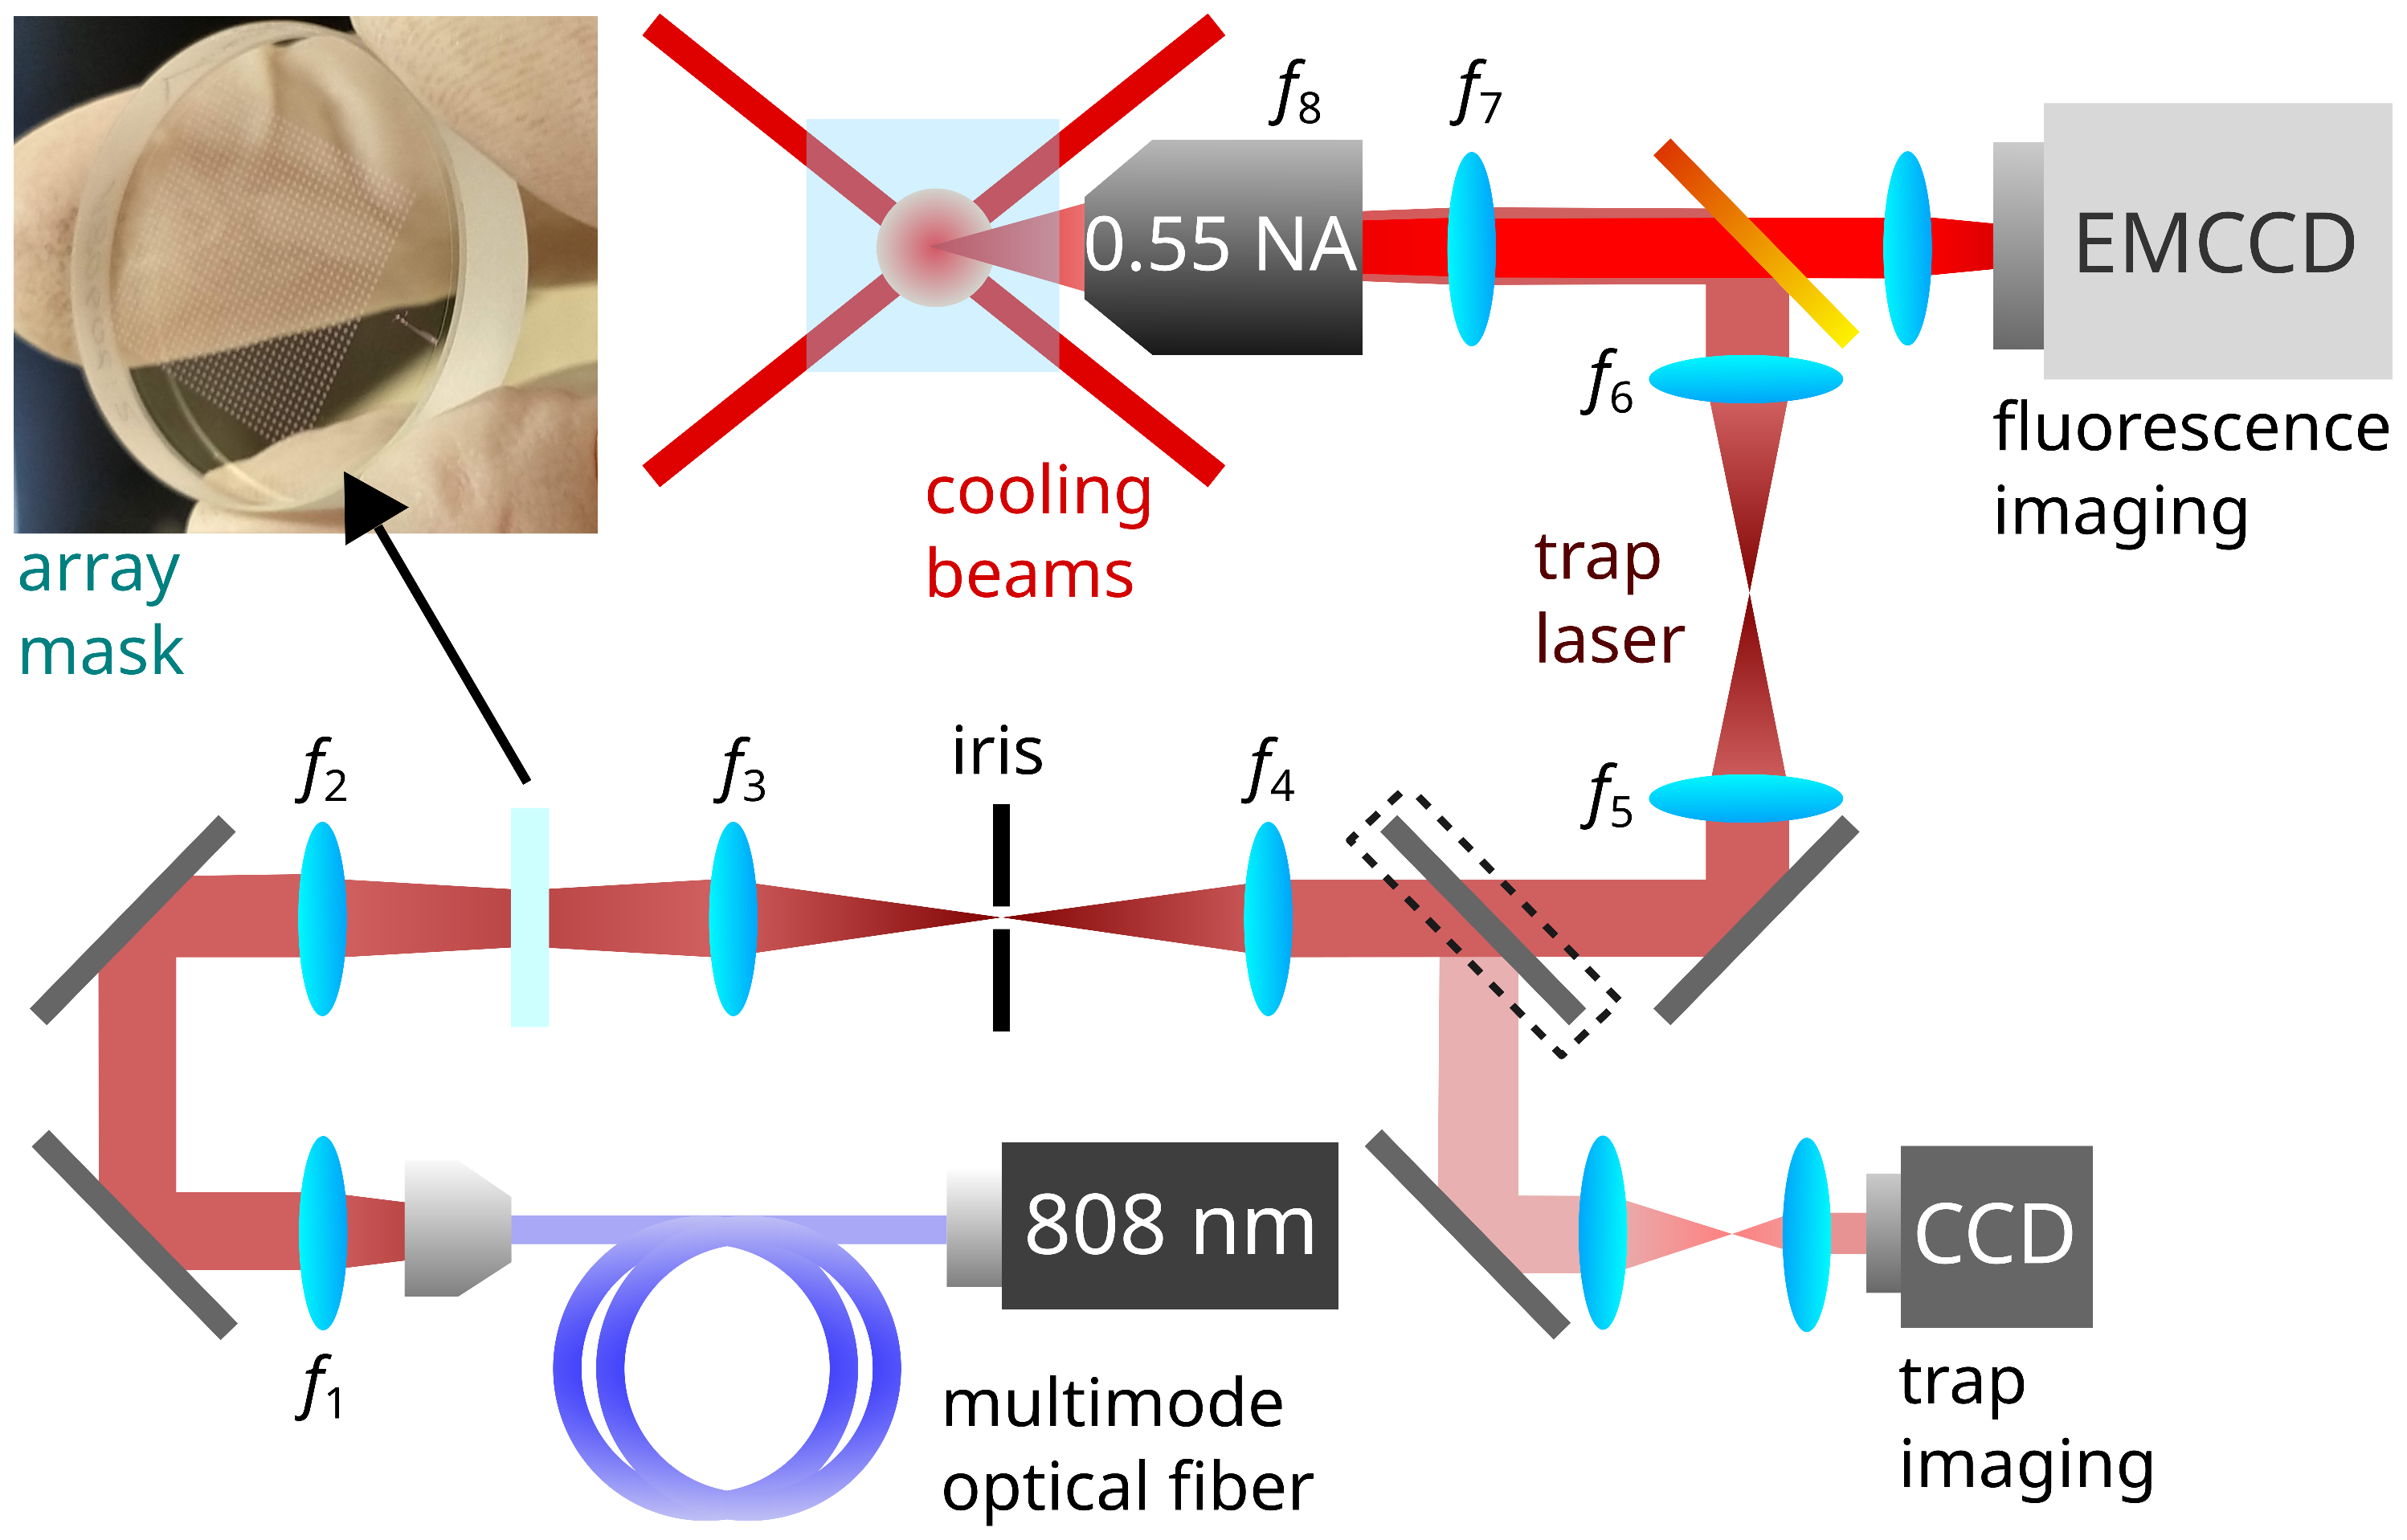
\includegraphics[width=0.45\textwidth]{Images/figure2.eps}
    \caption{Schematic of the experimental apparatus for trapping laser-cooled cesium atoms in a dark trap array made with a broadband, spatially multimode 808 nm laser. Atoms are loaded into a magneto-optical trap (MOT), then transferred into a blue-detuned dark trap array which overlaps the MOT. The trap array pattern is formed using a passive optical mask and $4f$ filtering scheme, and the trap is imaged onto the atoms using a 0.55 NA custom objective. The dashed outline denotes a removable mirror which is used for imaging the trap at low power onto a CCD camera. An EMCCD camera captures 852 nm fluorescence from the atoms, which is collected through the same objective lens used for focusing the trap light and picked off with a long-pass dichroic. The labeled lenses have focal lengths $f_{1-8} = (4.5,500,250,75,200,30,150,22.8)$ mm.}
    \label{fig:schem}
\end{figure}

For a Gaussian beam with waist parameter $w_0$ we have $\epsilon_{\perp}=2 / w_0^{2}, \epsilon_{\|}=\lambda^{2}/(\pi^{2} w_0^{4}) = 1/z_R^2$. The bright aG has similar atom distributions but with numerical corrections close to unity. The results for Gaussian, aG, and dark aG potentials are summarized in Table \ref{tab:params}.

For the dark aG trap, the potential is dominated by a quartic term to lowest order in the radial direction. Using the Virial theorem again, we obtain 
\begin{equation}
    \begin{gathered}
    \langle \rho^4 \rangle = \frac{2}{3}\frac{k_B T}{U_0 \epsilon_{\perp}}\\
    \sigma_{\rho} = \left(\frac{2}{3}\frac{k_B T}{U_0 \epsilon_{\perp}} \right)^{1/4}
    \end{gathered}
\end{equation}
where $\epsilon_{\perp}$ is the coefficient of the quartic term in the radial expansion of the potential.

In practice, the radial and axial confinement provided by a trap potential is found by a parametric heating experiment to deduce the vibrational frequencies of the trapped atoms. These are well defined along directions for which the potential is harmonic to lowest order. For a trap which closely approximates a Gaussian potential of waist $w_0$, with trap depth $U_0$ for an atom of mass $m$, we have 
\begin{equation}\label{eq:harmonic_freqs}
    \begin{gathered}
    \omega_{\rho} = \frac{2}{w_0}\sqrt{\frac{U_0}{m}}\\
    \omega_z = \frac{1}{h z_R}\sqrt{\frac{2 U_0}{m}}
    \end{gathered}
\end{equation}
For a perfect Gaussian beam, $h=1$. For the bright aG beam, which diverges somewhat slower in the axial direction, $h=1.307$, and for the dark aG trap $h=0.997$. In the case of the dark aG trap, the radial profile is dominated by a quartic term, so the radial motion of trapped atoms will obey the unforced Duffing equation \cite{Kovacic2011}. Hence, a particular vibrational frequency is not well-defined in this case. A summary of the trap frequencies and spatial confinement is given in Table \ref{tab:params}.

\newpage
\begin{sidewaystable} % don't use htb placement command!
% \begin{table*}[!th]
    \centering
    \begin{tabular}{|c|c|c|c|}
    \hline
    Parameter & Gaussian & Bright aG & Dark aG \\
    \hline \T
    $I(\rho,0)/I(0,0)$ & $1 - 2\big(\frac{\rho}{w_0}\big)^2 + 2 \big(\frac{\rho}{w_0}\big)^4 - ...$  & $1 - 2\big(\frac{\rho}{w_0}\big)^2 + 1.79 \big(\frac{\rho}{w_0}\big)^4 - ...$ & $ \big(\frac{\rho}{w_0}\big)^4 - ...$ \B \\
    \hline
    \T    
    $I(0,z)/I(0,0)$ & $1 - \big(\frac{z}{z_R}\big)^2 + \big(\frac{z}{z_R}\big)^4 - ... $ & $1 - 0.585 \big(\frac{z}{z_R}\big)^2 + 0.166 \big(\frac{z}{z_R}\big)^4 - ...$ & $ 1.01\big(\frac{z}{z_R}\big)^2 - 0.330 \big(\frac{z}{z_R}\big)^4 + ...$ \B \\
    \hline \T
    $\omega_{\rho}$ & $\frac{2}{w_0}\sqrt{\frac{U_0}{m}}$ & $\frac{2}{w_0}\sqrt{\frac{U_0}{m}}$ & ill-defined \B \\
    \hline \T
    $\omega_z$ & $\frac{1}{z_R}\sqrt{\frac{U_0}{m}}$ & $\frac{1}{1.307z_R}\sqrt{\frac{U_0}{m}}$ & $\frac{1}{0.997 z_R}\sqrt{\frac{U_0}{m}}$ \B \\
    \hline \T
    $\sigma_{\rho}$ & $w_0\big(\frac{k_B T}{2U_0}\big)^{1/2}=0.22~\mu$m & $w_0\big(\frac{k_B T}{2U_0}\big)^{1/2}=0.22~\mu$m & $w_0\big(\frac{2}{3} \frac{k_B T}{U_0}
    \big)^{1/4}= 0.28~\mu$m \B \\
    \hline \T
    $\sigma_z$ & $z_R\big(\frac{k_B T}{2U_0}\big)^{1/2}=0.87~\mu$m & $1.307 z_R\big(\frac{k_B T}{2U_0}\big)^{1/2}=1.14~\mu$m & $0.997 z_R\big(\frac{k_B T}{2U_0}\big)^{1/2}=0.87~\mu$m \B \\
    \hline
    \end{tabular}
    \caption{Comparison of normalized intensity profiles $I$, atom distribution standard deviations $\sigma$, and vibrational frequencies $\omega$ for the bright and dark aG ($t_a=0.287$) trap potentials, and a standard Gaussian bright trap. For ease of comparison, the expressions have all been cast in terms of the best-fit Gaussian waist $w_0$ and corresponding $z_R$. Numerical values for the standard deviations are given using $\lambda = 808$ nm and $w_0=1~\mu$m, and a ratio of atom kinetic energy to trap potential $k_B T/U_0 = 1/10$.}
    \label{tab:params}
% \end{table*}
\end{sidewaystable}
\newpage 

\begin{figure*}[!t]
    \centering
    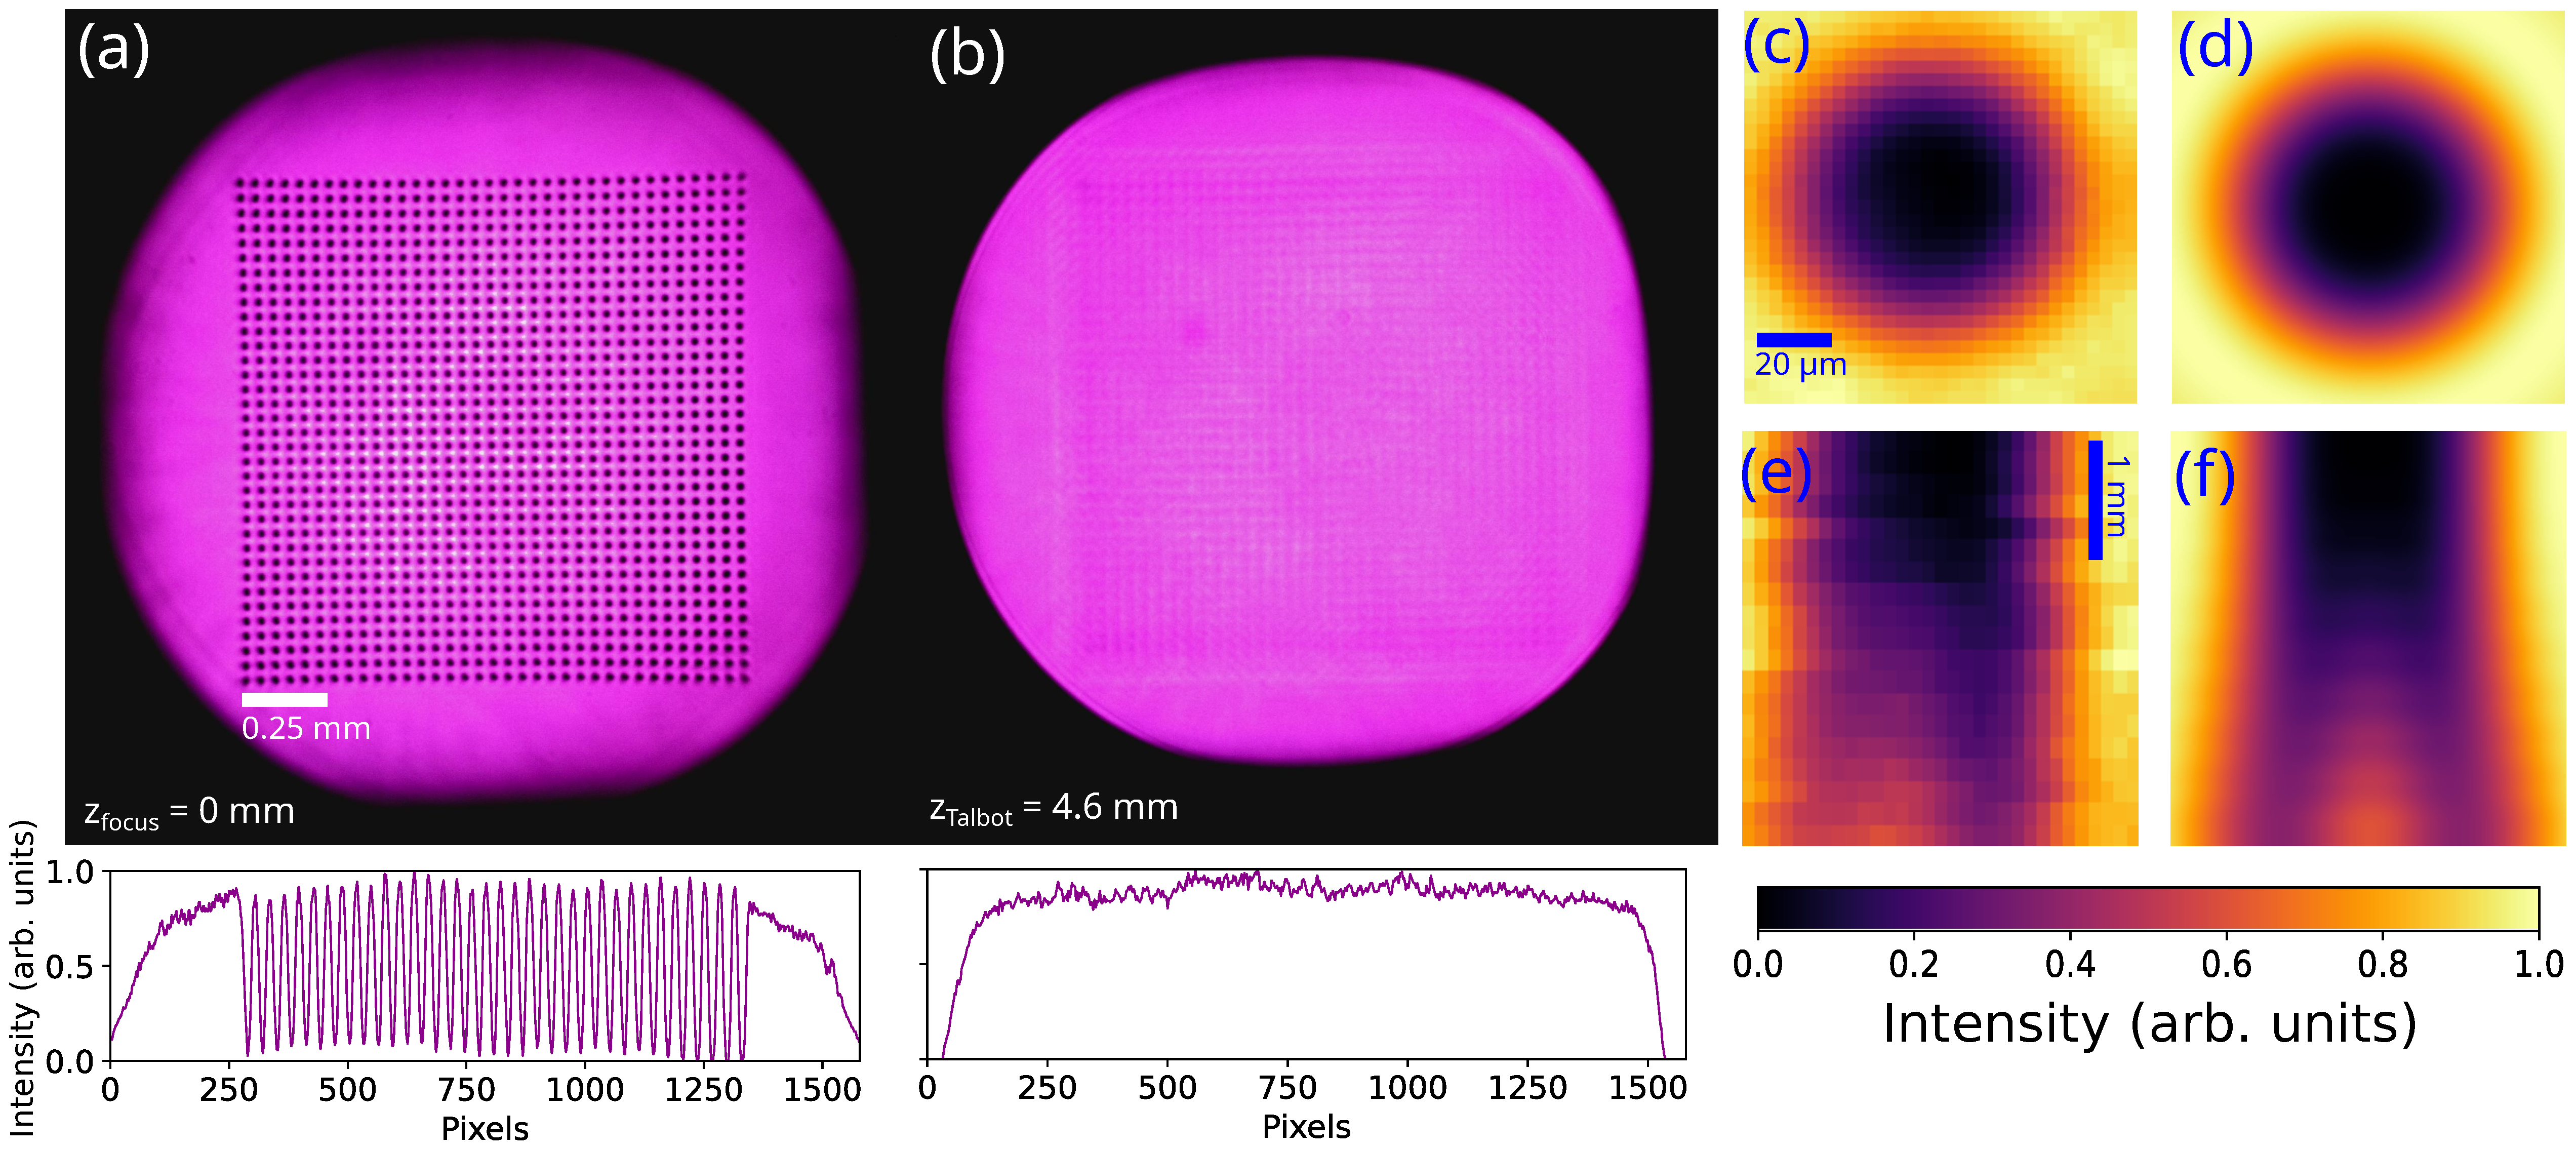
\includegraphics[width=1\textwidth]{Images/figure3.eps}
    \caption{Dark trap intensity profile with broadband, spatially multimode light. \textbf{(a)} The focal plane of traps imaged onto a CCD, formed with a $4f$ filtering system with a magnification of 1/10, giving an array period of $43~\mu$m in the imaging plane. For the $\lambda= 805~ $nm light used, \textbf{(b)} the Talbot plane is located at $z=4.6$ mm, where the re-imaged traps have been strongly suppressed. \textbf{(c)} and \textbf{(e)} show a single trap site with 808 nm multimode light projected on the focal plane and along the propagation plane intersecting $\rho=0$. For qualitative comparison, \textbf{(d)} and \textbf{(f)} show numerical simulations of the trap using coherent single mode light}
    \label{fig:trap_intensity}
\end{figure*}

\section{Experiment} \label{sec:exp}

We demonstrate the proposed method of creating a blue-detuned dark trap array with up to 1225 sites for trapping single Cs atoms, and compare the use of an incoherent laser versus a coherent laser. The trap array is formed using a commercially fabricated (by LaserOptik) custom mask consisting of a $35 \times 35$ grid of partially transmitting disks of radius  $a=100~\mu$m ($|t_a|^2 = 0.49$; see Sec. \ref{sub:profiles}) and spatial period $d=430~\mu \textrm{m}$, positioned on a 25.4 mm diameter glass blank AR coated for a design wavelength of 825 nm. The experimental setup, shown in Fig. \ref{fig:schem}, is the same for trapping with both coherent and incoherent lasers except for the lasers themselves and the optics that precede the array mask. The array mask and $4f$ telescope is followed by an intermediate pick off for imaging the trap intensity with a magnification of roughly $1/10$, and the array is imaged into the science chamber to have a spatial period of 3 $\mu$m at the atoms. We emphasize that for a given array mask, the period of the array at the atoms and the trap depth can be tuned by changing the magnification of the imaging system.

\subsection{Incoherent trap}\label{sub:incoherent}
\begin{figure*}[!t]
    \centering
    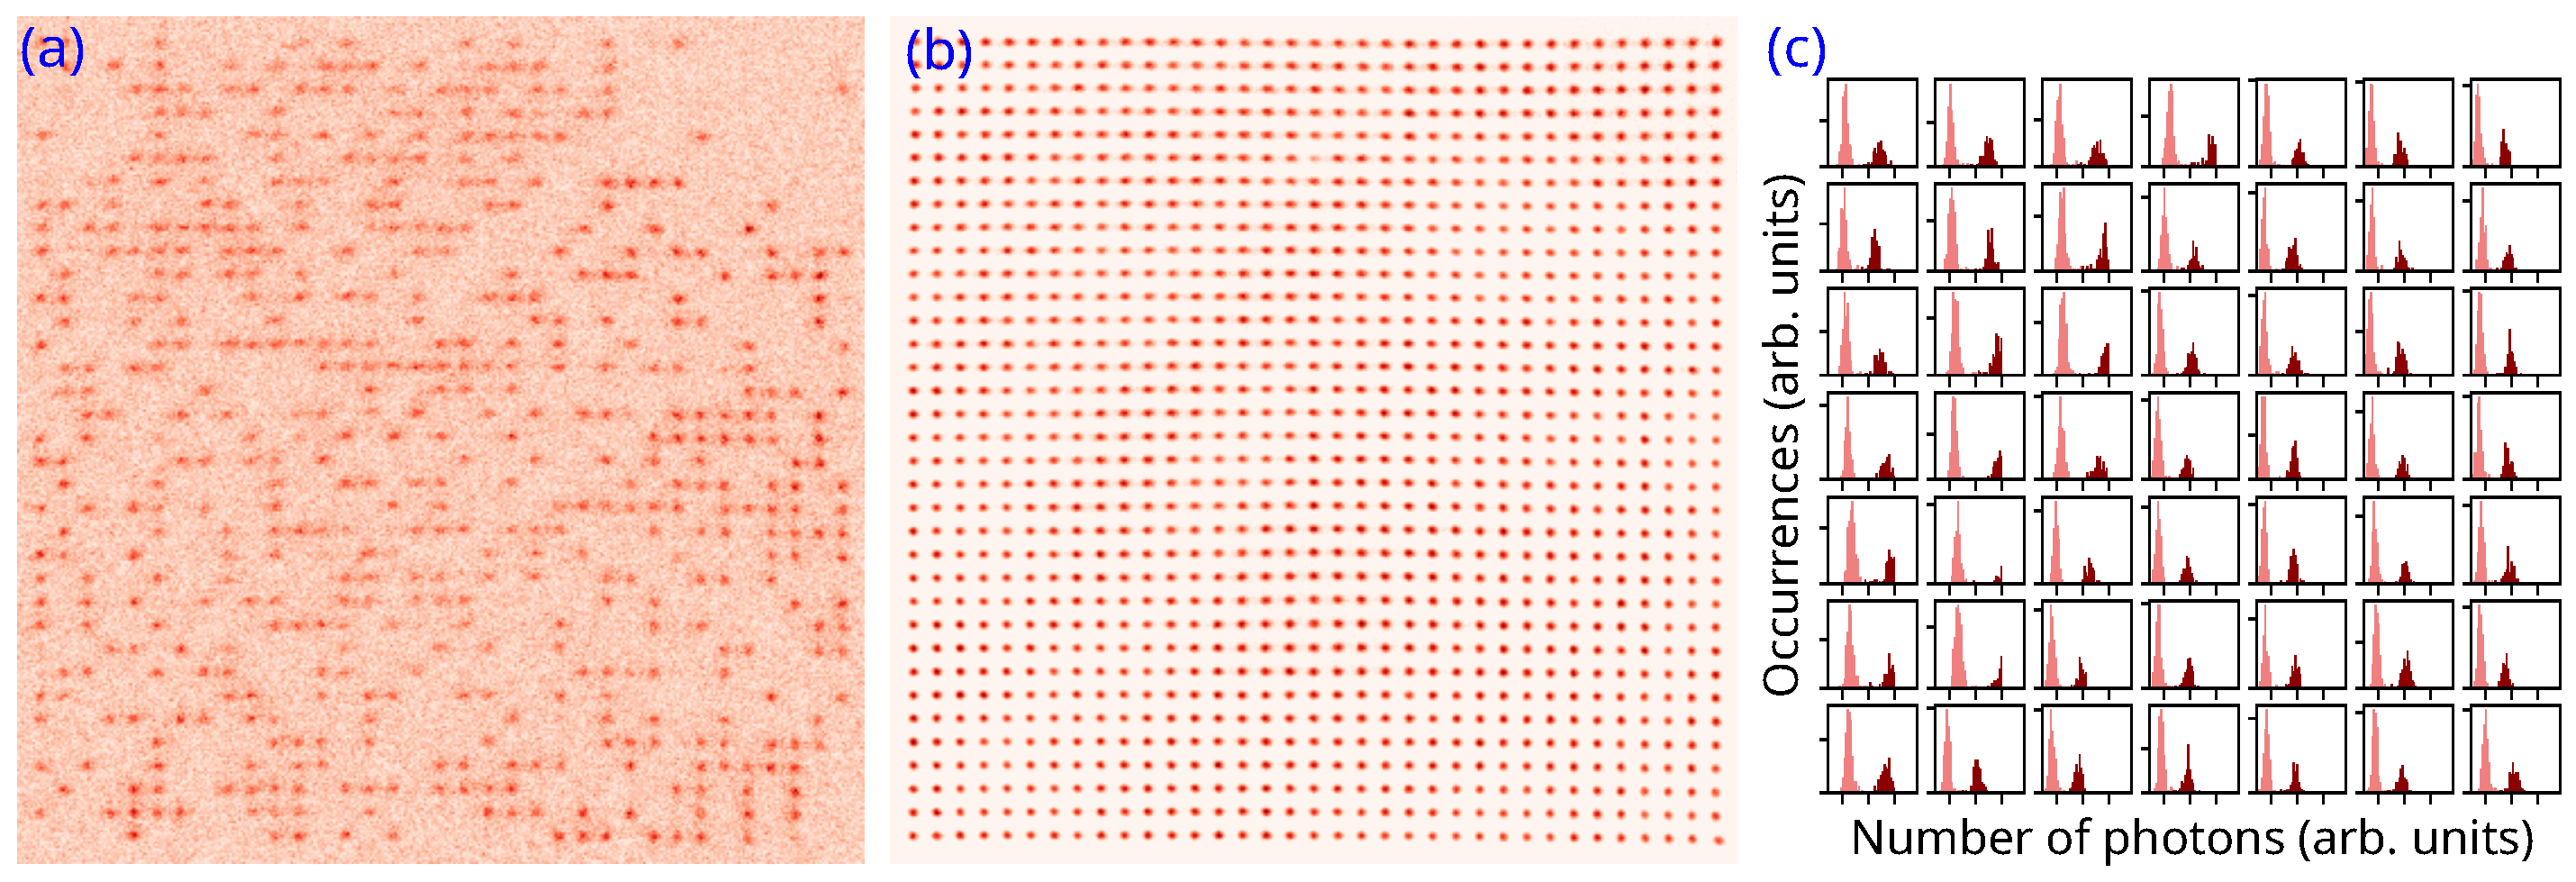
\includegraphics[width=\textwidth]{Images/figure4.eps}
    \caption{Single atom loading in a 1225-site array of dark traps formed with a broadband, spatially multimode laser. See section \ref{sec:exp}. \textbf{(a)} Single fluorescence image, showing stochastic loading of the trap array. The spacing between trap sites is about $3~\mathrm{ \mu m}$. \textbf{(b)} Averaged fluorescence image processed with independent component analysis. (see Sec. \ref{sub:imaging}). \textbf{(c)} Histograms of photocounts from regions of interests defined for the central 49 sites in (a),(b), showing the well-separated background (pink) and single atom (dark red) distributions.}
    \label{fig:bigarray}
\end{figure*}
First, we present single atom trapping in a 2D 1225-site  dark trap array with a high power spatially multimode, broadband 808 nm laser (Aerodiode CCMI, 35 W), which is blue-detuned with respect to  the Cs D-lines. Going forward, we will simply refer to this laser as the ``incoherent'' laser. 

The incoherent light is used in order to form the optical trap array without incurring the formation of Talbot plane traps, as shown in Fig. \ref{fig:trap_intensity}. For an explanation of the dominant mechanism in destroying the Talbot interference, see Sec. \ref{sec:talbot}. The entire array mask was illuminated and imaged onto a CCD following a $4f$ filtering setup. In order to have uniform trap depths across the array, it is crucial to uniformly illuminate the mask, which we do by re-imaging the core of a $200~\mu$m multimode fiber on to the mask. This is a good approximation to illuminating the mask with a top-hat intensity profile. An adjustable iris was used as the spatial filter in the $4f$ setup, and tuned to a radius of about 0.5 mm to minimize the trap center intensities as viewed on a CCD camera. To characterize the trap, we begin by stochastically loading single Cs atoms from a MOT into the array, for which we observe up to about 50$\%$ filling of the array. The trap light is switched on by controlling the laser current, instead of using an AOM, due to poor diffraction efficiency with the multimode light. Fluorescence images of atoms loaded into the array are shown in Fig. \ref{fig:bigarray}, with an average single atom loading rate in excess of 30$\%$ for the data shown. The loading rate  observed with coherent trapping light, discussed below, was about 50$\%$. We attribute the increase in loading rate with coherent light to the difference in relative intensity noise (RIN) between the two lasers (see Sec. \ref{sub:lifetime}). 

The axial and radial frequencies of the atoms in the trap were measured to be about 6 kHz and 34 kHz, respectively\footnote{In the publication, there was a typo, so the radial frequency was given to be 44 kHz by mistake.}, by parametric heating from modulating the laser current with a sinusoidal source. For the particular mask used, we expect a trap which diverges faster in the axial direction compared to the expansion given in eq. (\ref{eq:Iag_dark2}), providing tighter axial confinement. For the radial direction, the trap closely matches a harmonic potential, and therefore the standard radial frequency relation (see eq. (\ref{eq:harmonic_freqs})) for a harmonic potential applies (see Sec. \ref{sub:profiles}). Hence there are three free parameters in the pair of trap frequency equations: the best-fit Gaussian waist $w_0$, trap depth $U_0$, and divergence parameter $h$. It is not straightforward to predict $h$ due to the unknown $M^2$ for the incoherent light, so we use the two trap frequencies to solve for $h$ and $U_0$, given a value of $w_0$ found using the known imaging magnification and a calibrated fit of the trap intensity. For a fit waist of 1.6 $\mu$m, the trap frequencies imply $U_0/k_B=462 ~\mu$K and $h=0.647$. The polarizability of the Cs $6\text{S}_{1/2}$ states is
$\alpha_0 = 0.66\times10^{-6} ~\mu\text K/(\text W/\text m^2)$ at 808 nm, and the estimated intensity at the atoms is $7.06 \times 10^8~\text W/ \text m^2$ (with about 20 W of light), giving an expected trap depth of $U_0/k_B=466 ~\mu \text K$. This agrees with the value implied by the trap frequencies to within a few percent, and $h$ is of the same order as the numerical prediction with coherent light. 
The observed atom lifetime in the incoherent trap was about 40 ms, in comparison to about 5 s measured with the coherent trap to be discussed next. We attribute this difference to the RIN of each laser (see Sec. \ref{sub:lifetime}). Nevertheless, we emphasize there is nothing fundamentally prohibitive for obtaining reasonable trap lifetimes in  multimode optical traps \cite{WHung2015,Povilus2005}. Moreover, intensity-noise limited trap lifetimes can be significantly improved  using well developed noise reduction techniques such as the method used in \cite{YuWang2020}, which uses an AOM and EOM for slow and fast noise reduction, respectively. We note that the poor diffraction efficiency of an AOM with multimode light is not a barrier to intensity stabilization as it was to using an AOM as an optical switch. This is because using an AOM for intensity stabilization requires dumping a relatively small amount of power into the diffracted order. Furthermore, the intensity stabilization scheme in \cite{YuWang2020} could be modified to use two EOMs instead of one AOM and one EOM, if diffraction efficiency is a concern. 

\subsection{Coherent trap}\label{sub:coherent}
The same trap characterization experiments were repeated using a coherent 825 nm laser (Moglabs MSA003 tapered amplifier), where the only change to the experimental setup was the optics for collimating the trap light before the array mask. The mask was illuminated using a Gaussian beam which was collimated after being spatially filtered by a single mode fiber. Despite the Gaussian illumination of the mask, which leads to a varying trap depth across the array, we still observe traps which go completely or near completely dark across the array, indicating that uniform mask illumination is not  strictly required.

\begin{figure*}[h]
    \centering
    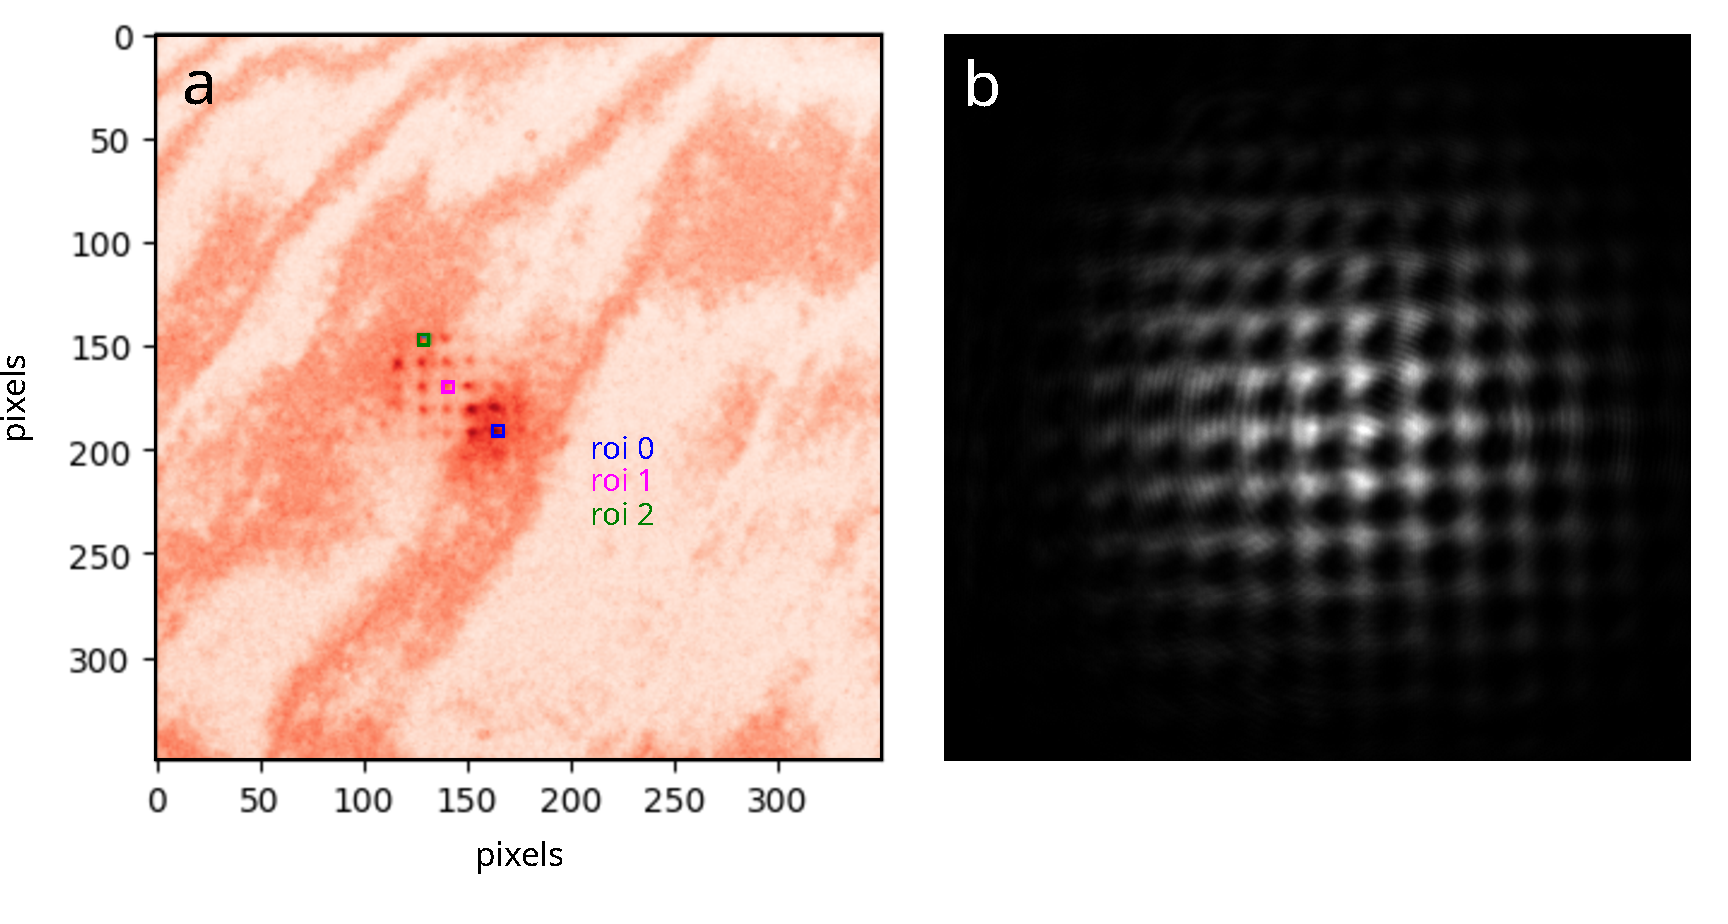
\includegraphics[width=\textwidth]{Images/coherent_trap_intensity_and_atoms.pdf}
    \caption{(\textbf{a}) Averaged image of trapped single cesium atoms in the coherent trap array and (\textbf{b}) an image of the corresponding trap intensity pattern in the intermediate imaging plane. The colored rectangles in (\textbf{a}) show the regions of interest (ROIs) used in experiments, where ROIs 0 and 1 are the sites used for the reported trap frequency and lifetime measurements. Fringes in (\textbf{b}) are from the camera sensor, and the wavy pattern in (\textbf{a}) is due to varying gain across the sensor array on the Hamamatsu camera used,  attributed to the camera's age.}
    \label{fig:coherent_trap_and_atoms}
\end{figure*}


Again, we characterize the confinement by measuring the trap frequencies and trap lifetime. The trap depth for different sites varies according to the Gaussian intensity envelope across the array. We will therefore restrict our analysis to values near the center of the array, where the traps are deepest. The peak intensity at the atoms is given approximately by $I = 2P/\pi w_{\text{env}}^2$, where $P=260$ mW is the laser power and $w_{\text {env}}=12~\mathrm{ \mu m}$ is the Gaussian envelope waist at the atoms. This yields about 20 to 25 sites which are deep enough for trapping. To parametrically heat the atoms, the trap light intensity was modulated by varying the RF power to an AOM placed before the single mode fiber delivering light to the $4f$ filtering setup. We measure radial and axial frequencies of about 52.5 kHz and 7.2 kHz, respectively (Fig. \ref{fig:coherent_frequencies_and_lifetime}). The rate of axial divergence, which is faster than that of a Gaussian beam, has a divergence parameter $h=0.65$ predicted by a Fresnel diffraction simulation for the parameters of the mask used (see \ref{sec:sensitivity}). Assuming this value of $h$, the trap frequencies imply a trap depth of $1.4$ mK and waist $w_0=1.81~\mu$m. This waist is consistent with the value of $1.89~\mu$m deduced from fitting the trap in the intermediate imaging plane to within a few percent, and the trap depth is within our uncertainty in measuring the intensity. Lastly, the trap lifetime was found to be nearly 5 s, measured in the same site for which we report the trap frequencies.

\begin{figure*}[h]
    \centering
    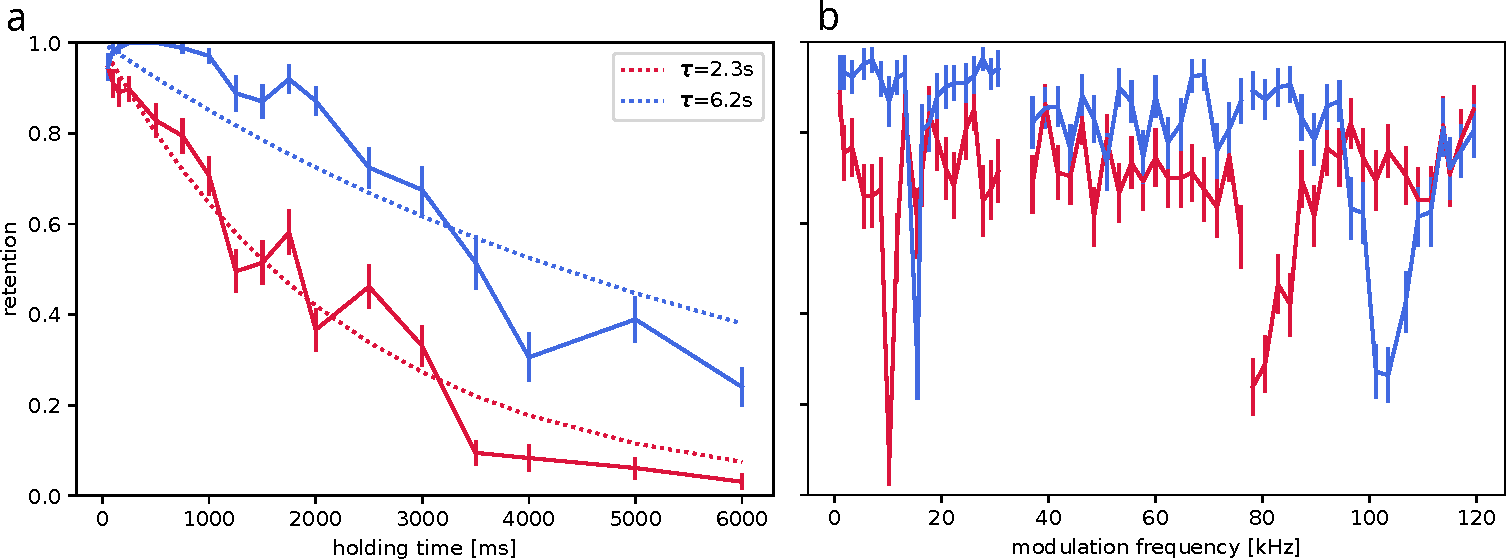
\includegraphics[width=\textwidth]{Images/coherent_trap_lifetime_and_resonances.pdf}
    \caption{(\textbf{a}) Coherent trap vibrational frequencies and (\textbf{b}) lifetimes. The blue (red) curves in each corresponds to data from the same trap site in the array, and the error bars denote $\pm1$ standard deviation for the measurements. The values reported in the text come from the red. Discrepancies between the frequencies and lifetimes are attributed to the difference in trap depth across the array, as a Gaussian intensity profile was used to illuminate a subset of only $\sim$25 apertures on the array mask.}
    \label{fig:coherent_frequencies_and_lifetime}
\end{figure*}
We note that the secondary arrays of traps formed due to the Talbot effect with coherent light allows for creating a three-dimensional trap array, which may be advantageous for multi-dimensional architectures\cite{YWang2016,Barredo2018}.

% \section*{Disclosures}
% The authors declare no conflicts of interest.

% \section*{Data Availability Statement}
% Data underlying the results presented in this paper are not publicly available at this time but may be obtained from the authors upon reasonable request.

% \section*{Acknowledgments}
% This material is based upon work supported by the
% U.S. Department of Energy Office of Science National
% Quantum Information Science Research Centers as well as support from NSF Award 2016136 for the QLCI center Hybrid
% Quantum Architectures and Networks, NSF award 1806548,  and U.S. Department
% of Energy, Office of Science, Office of High Energy Physics,
% under Award No. DE-SC0019465.  

% \section*{Supplemental document}
% See Supplement 1 for supporting content. 

% \bibliography{rydberg,optics,qc_refs,atomic,saffman_refs}
% %\bibliography{rydberg,optics,qc_refs,atomic,bibliography}
% % Produces the bibliography via BibTeX.

% \appendix

\section{Robustness of $4f$ filtered traps}\label{sec:sensitivity}

A natural question to pose is to what extent the $4f$ filtering approach to generating traps is sensitive to parameters, such as the mask transmission amplitudes, Fourier filter radius, and the intensity profile used to illuminate the mask. Here we address this for the case of generating dark traps. The metric we find most useful is simply to quantify the relative intensity at the centers of the traps, that is, $I_2(0,0)/I_0$ (eq. (\ref{eq:Iag_dark})). The derivation of the dark trap found the condition for completely dark traps given zero relative phase between the mask aperture and background transmission amplitudes, $t_a,t_b$, and a choice of filter radius $b$ corresponding to blocking the Airy disk beyond the first minima. 
\begin{figure}[!ht]
    \centering
    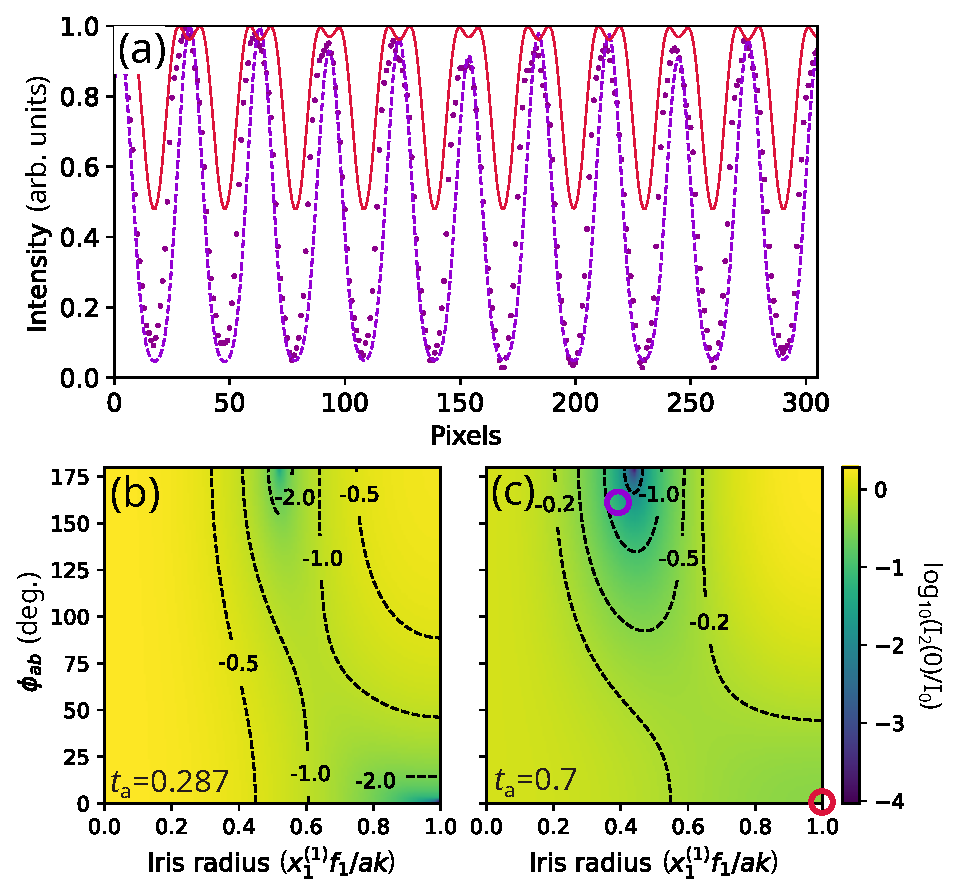
\includegraphics[width=0.6\textwidth]{Images/figure5.eps}
    \caption{Numerical analysis of dark aG trap profile dependence on relative mask phase $\phi_{ab}$ and Fourier filter (iris) radius. The iris radii here are given as dimensionless by dividing by the value used in the derivation in the main text, $b=x^{(1)}_1 f_1/a k$. \textbf{(a)} Trap profile data (purple points) from Fig. \ref{fig:trap_intensity}a compared to two Fresnel diffraction calculations: one with parameters which give a similar profile (purple dashes), and one with parameters corresponding to the expected trap given the specified parameters of the mask used (red line). Both parameter sets  use $f_1=500$mm,$f_2=50$mm, $\lambda=805$nm, with the former using ($\phi_{ab}$, iris radius) = ($160^{\circ}$,0.4), and ($0^{\circ}$,1) for the latter. \textbf{(b)} and \textbf{(c)} show the dark trap center intensity (log scale) versus $\phi_{ab}$ and iris radius. The choices of $\phi_{ab}$ and iris radius used to generate the numerical curves in (a) are marked with rings of the same color in (c).}
    \label{fig:idark_vs_phi_b}
\end{figure}

However, the trap can be made near completely dark for other choices of these parameters. Fig. \ref{fig:idark_vs_phi_b} shows the trap center intensity for two values of $t_a$ (and $t_b=1$), as a colormap versus the relative phase $\phi_{ab}$ between $t_b,t_a$ and the Fourier filter or iris radius cast in dimensionless units. For $t_a=0.287$, as derived as optimal above, we see the trap remains dark to within about $10 \%$ for up to around 20 degrees of relative mask phase, indicating the robustness of the design with respect to deviance in parameters from manufacturing of a real mask.

\section{Tighter traps with alternative Fourier plane masks}\label{sec:tighter}
It is possible to create tighter trap profiles than those presented in the main text, by replacing the simple Fourier plane iris with more complicated amplitude or phase masks. For example, a higher efficiency (eq. (\ref{eq:brighteff})) bright trap can be created by using a modified Fourier plane amplitude mask which transmits certain higher spatial frequency bands. This amounts to adding spatial notch filters, i.e. transmitting rings, to a low-pass filter as used in the main text. It can be shown that the transparent rings should have inner and outer radii equal to $f_1 x_{2n}^{(1)}/(ak)$, $f_1 x_{2n+1}^{(1)}/(ak)$ respectively, for the $n^{th}$ ring from the center, for $n>1$. The central aperture has radius $f_1 x_{1}^{(1)}/(ak)$. This type of filter, which we refer to as a Fresnel zone filter, is shown with  only one ring in Fig. \ref{fig:zonefilter} alongside the resulting trap profiles compared to those of a standard aG beam. It is apparent from the figure that the resulting traps have much stronger confinement than is obtained with the simple low pass filter. Compared to the bright aG trap, the trap generated with the zone filter has roughly 1.9 times higher efficiency (corresponding directly to the trap depth), with about 2.2 and 10 times tighter confinement in $\rho$ and $z$, respectively. The zone filter does introduce weak secondary traps away from the origin. Atom trapping in the secondary traps can be avoided, either by slowly increasing the trap power during the loading phase, or by using atom rearrangement techniques to place atoms in the central trap. 

\begin{figure}[!ht]
    \centering
    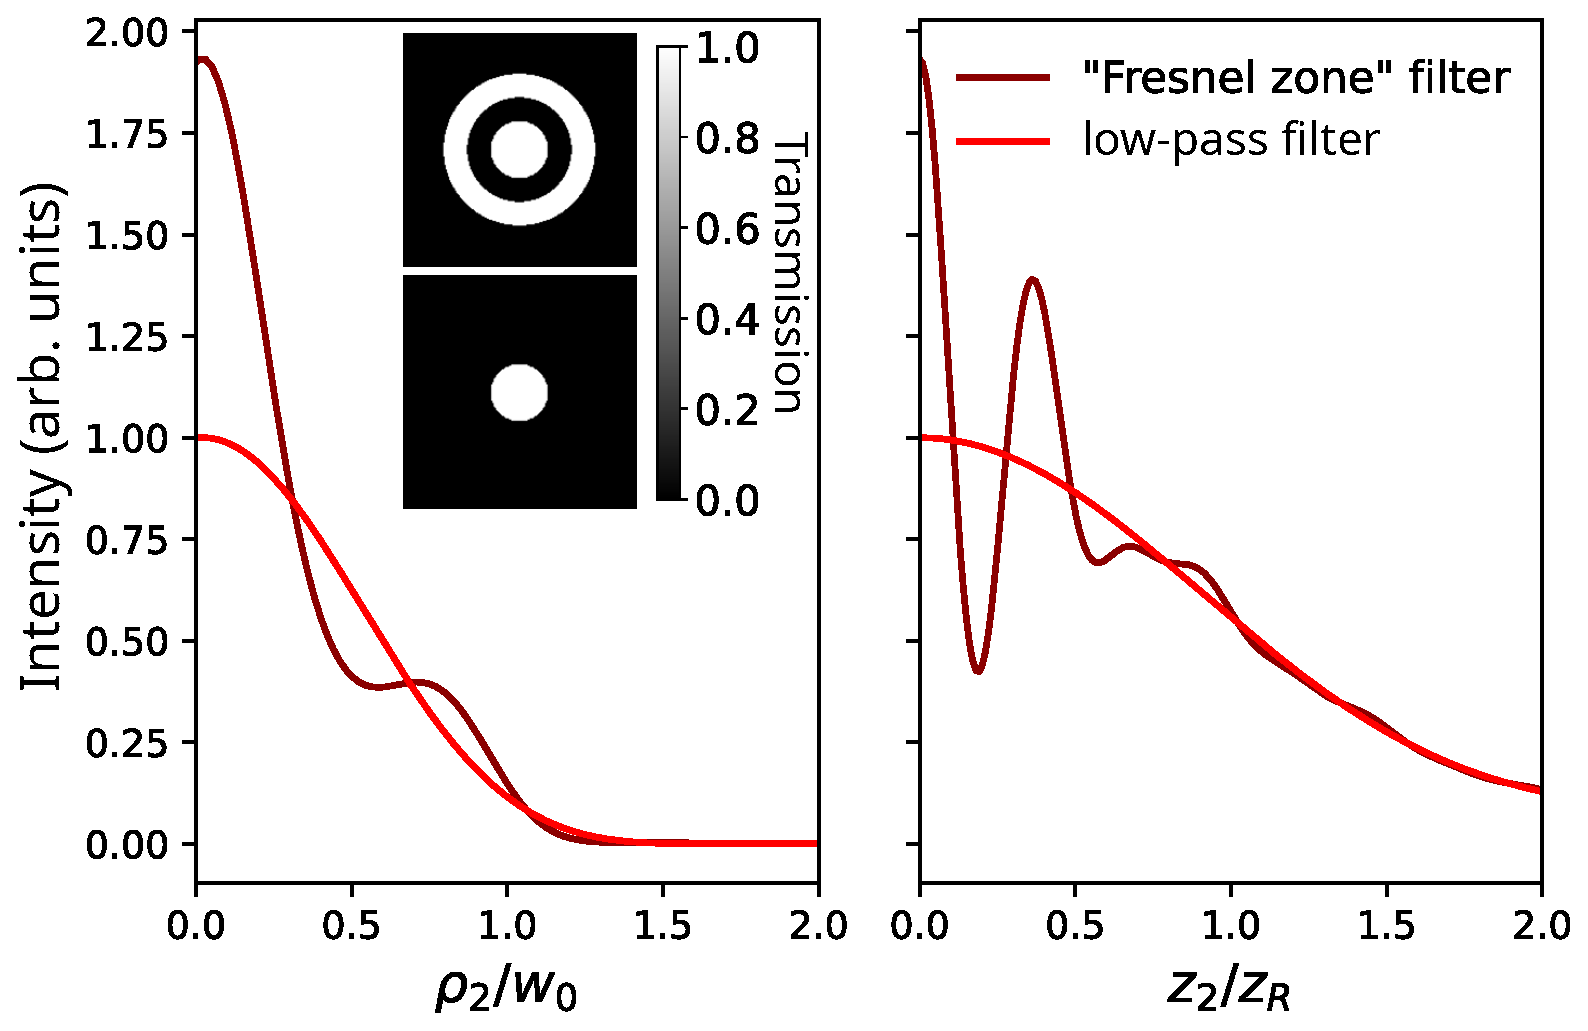
\includegraphics[width=0.6\textwidth]{Images/figure6.eps}
    \caption{Comparison between an aG beam produced with a low-pass Fourier filter (see main text) and a modified version using a "Fresnel zone" Fourier filter. The horizontal axes are scaled to the best fit Gaussian waist $w_0$ and corresponding Rayleigh range $z_R=\pi w_0^2/\lambda$ for the aG beam. The two Fourier filter variants are shown in the inset, and the radii of the transmitting rings and central aperture are given in the text.}
    \label{fig:zonefilter}
\end{figure}

\section{Talbot Trap Mitigation}\label{sec:talbot}

In cold atom experiments using periodic optical trap arrays, it is a known problem that secondary traps, which form due to the Talbot effect, lead to out-of-focus trapped atoms. This contributes additional background in fluorescence measurements used for atom state detection and atom rearrangement \cite{graham2019}. The Talbot effect is a well-known phenomenon in optics, in which a field which is spatially periodic in the transverse plane will be reimaged after propagating a distance equal to 
\begin{equation*}
    z_{\text{Talbot}} = \frac{2d^2}{\lambda}
\end{equation*}
where $d$ is the transverse spatial period of the field and $\lambda$ is the wavelength of the field. Numerical simulations of the first Talbot planes for dark and bright trap arrays are shown in Fig. \ref{fig:talbotcompare} We propose a solution using a spatially and spectrally incoherent laser field. 
\begin{figure}[!th]
    \centering
    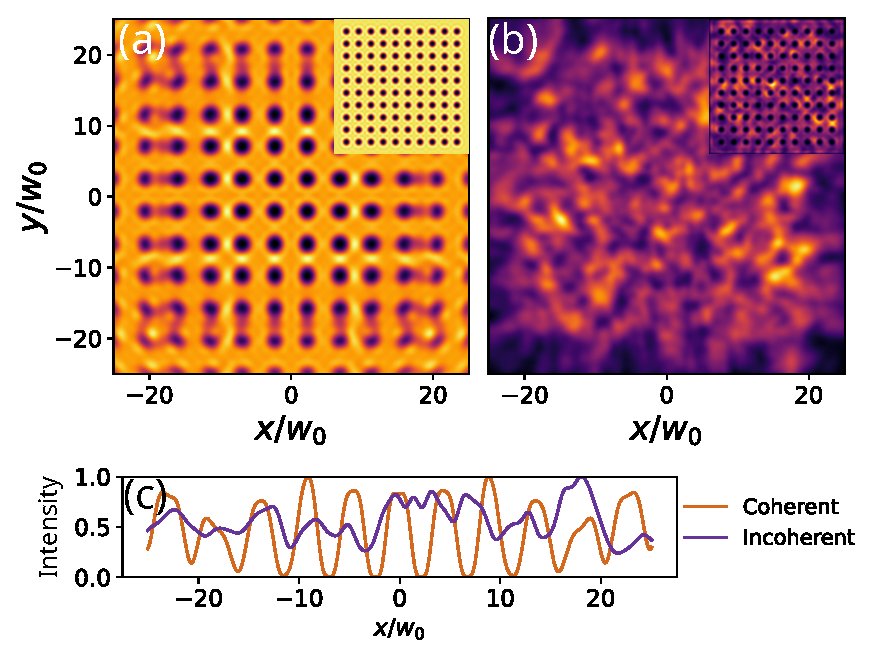
\includegraphics[width=0.6\textwidth]{Images/figure7.eps}
    \caption{Comparison of simulated Talbot plane trap formation for a 10 by 10 dark aG array formed with \textbf{(a)} spatially coherent monochromatic light and \textbf{(b)} spectrally and spatially incoherent field. For the incoherent light, 21 frequency components spanning $\Delta \lambda_{\text{FWHM}} = 3$ nm, each with 200 Hermite-Gaussian modes with random phases. The insets show the the focal plane intensity. The plot axes are scaled to the best fit Gaussian waist, $w_0=0.943 a(f_2/f_1)$. \textbf{(c)} Line profile comparison of a row of traps from (a) and (b), showing the washed out Talbot interference for the multimode light. For both simulations, $\lambda_0=825$ nm, $d=430~\mu$m, and $a=100~\mu$m, and a magnification of 1/100.}
    \label{fig:talbotcompare}
\end{figure}

The Talbot effect can be mitigated by use of a spatially multimode laser, which has a limited spatial coherence. In what follows we will limit the numerical analysis to the case of a dark trap array, although much of the discussion is equally applicable to bright traps. In addition to being spatially multimode, it is desirable to have many frequency components as well. This ensures that the bright region of the trap does not exhibit a speckle pattern, which could create additional unwanted traps. This section will outline results of numerical simulation. The experimental confirmation of these predictions shown in Sec. \ref{sec:exp} of the main text. 

The models presented here use Fresnel diffraction theory, which is readily computed using fast Fourier transform (FFT) algorithms that are available in modern programming languages \cite{kelly2014}. This modeling can be done efficiently on a typical laptop. For computational efficiency, the results presented below are for 10-by-10 trap arrays. All of the Talbot plane intensity plots shown are normalized to the respective peak focal plane intensity, to provide a clear sense of the relative trap depth. For the simulations discussed, the laser wavelength is $\lambda =825 $ nm, mask grid period $d=430~ \mu$m, mask spot radius $a=100~\mu$m, aperture transmission $t_a=0.287$. However, the results are presented in a way that is independent of the choice of parameters such as focal lengths and wavelength.

Let us first consider an array of optical traps formed by a laser which has many frequency components, but is spatially coherent. Far-off resonance optical traps do not require narrow-linewidth lasers, and hence the use of a free-running, broadband laser is feasible. Naively, we may assume that if the coherence length of the laser is less than the Talbot length of the trap array, the Talbot traps will be suppressed. To quantify how short the coherence length must be in order for the Talbot traps to be washed out, we need to consider 1) the axial displacement of the Talbot plane for a given $\Delta \lambda$ from the central trap wavelength $\lambda_0$, and 2) the axial depth of the Talbot traps. The depth of the Talbot plane is $\delta Z_{\textrm{Talbot}} \sim \pi w_0^2/\lambda$ where $w_0=0.947af_2/f_1$ is the waist of the trap (for the case of the bright array), and the amount that the Talbot plane is displaced for a change in $\lambda$ is $2 \Delta \lambda d^2/\lambda^2$. Combining these, we find that in order to displace the Talbot plane by half of its axial depth, we require a laser with a spectral full-width of 
\begin{equation}
    \Delta \lambda_{1/2} = \frac{\pi \lambda}{2} \frac{a^2}{d^2} \frac{f_2^2}{f_1^2}
\end{equation}
For $a=100~\mu$m and a magnification of $1/100$, a laser with a FWHM of more than 10 nm is required to sufficiently wash out the Talbot plane. Typically, even lower quality laser diodes have linewidths of at most a few nm, insufficient for mitigating Talbot trap formation for the trap parameters considered. However, as we will show, spectral incoherence still plays an important role in the demonstrated solution to the Talbot problem.

We find that a practical and cost-effective approach to mitigating Talbot traps is using a laser which is both spectrally and spatially incoherent, which are readily available at high power. By using a spatially  multimode field, there is no longer spatial coherence which is required for forming the Talbot planes. A monochromatic but spatially incoherent field, as can be made by passing a laser with a single spatial mode through a  multimode fiber, has a speckled intensity and hence is not a good solution for creating trap arrays. A spectrally and spatially  multimode field will, however, not be speckled. This is explained by thinking of each spectral component as having its own associated speckle pattern. These speckle patterns add incoherently, i.e. the intensities rather than the fields are summed, resulting in a more uniform intensity pattern.

We model spatially incoherent fields by summing Hermite-Gaussian fields $A_{i,j}$ from $A_{0,0}$ to some highest-order $A_{m,n}$, with each spatial mode being given a random phase pulled from a flat distribution.  This process is done for each spectral component of the field and scaled by $\sqrt{L(\nu, \nu_0)}$ where $L$ is the Lorentzian function describing the spectral width of the laser. Each speckle field is then propagated through the $4f$ array generator and the intensities at the output are summed, yielding the output shown in Fig. \ref{fig:talbotcompare}b.

\section{Experimental details}\label{sec:experiment}

\subsection{Array mask and observed trap profiles}\label{sub:profiles}
The experimental demonstration of the proposed trap design used a commercially fabricated array mask consisting of partially transmitting disks (what we have previously been calling ``apertures'') set on an AR-coated 1'' diameter glass blank. The requested transmission of the disks was $|t_a|^2=0.49\pm 0.04$, with a relative phase of $0 \pm 10 $ deg. between the disks and AR coated background, designed for $\lambda = 825$ nm. The disks have radius $a=100~\mu$m and arranged in a 2D square grid with spatial period $d=430~\mu$m. The expected trap profile for these mask parameters does yields traps which are only about 50$\%$ dark (Fig. \ref{fig:idark_vs_phi_b}a). However, given the observed nearly dark traps and numerical analysis, we infer that the relative phase imparted on the light between the fully and partially transmitting regions must be outside of the specified tolerance in order to explain the observed trap profiles. 

\begin{figure}[t!]
    \centering
    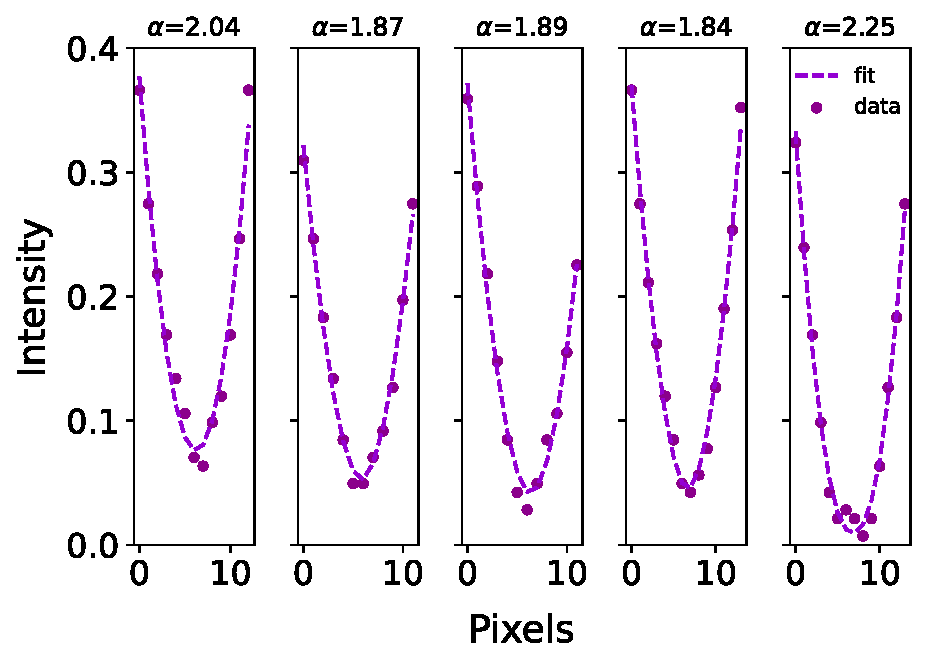
\includegraphics[width=0.6\textwidth]{Images/figure8.eps}
    \caption{A row of adjacent trap site profiles from the data shown in Fig. 2, where each site has been fit to a form $a\rho^\alpha+b$. The data was clipped above the $1/e$ intensity to ensure fitting to the lower order portions of the traps. It is clear that the experimentally observed radial profiles are nearly quadratic, rather than the quartic profiles expected for $t_a=0.287t_b$ with zero relative mask phase.}
    \label{fig:site_fits}
\end{figure}

Because a direct phase measurement of the array mask is difficult, we present numerical analysis to explain the observed trap profile. These results are summarized in Fig. \ref{fig:idark_vs_phi_b}. The observed traps can be made dark to within $10\%$ of the peak intensity by adjusting the iris radius. This constrains the possible values of $\phi_{ab}$ and iris radius that are consistent with the trap we observe. For example, a Fresnel diffraction calculation for $t_a=0.7$, iris radius $b=0.4x^{(1)}_1 f_1/a k$ and $\phi=160^{\circ}$, gives a result that agrees well the observed trap profiles (Fig. \ref{fig:idark_vs_phi_b}a, purple dashes). This choice of parameters is marked with a purple ring in Fig. \ref{fig:idark_vs_phi_b}b.

Moreover, the axial divergence rate of the trap is in good agreement with the measured trap frequencies. It can be shown that the quadratic term of the axial expansion for $\phi_{ab}=160^{\circ}$ and $b=0.4x^{(1)}_1 f_1/a k$ is equal to $2.356(z/z_R)^2$, giving a divergence parameter $h=1/\sqrt{2.356}=0.65$. This is an additional advantage conferred by the mask parameters, as the axial confinement is $\sim 30\%$ tighter compared to the expansion rate using $t_a=0.287$ and $\phi_{ab}=0$. As stated in the main text, the measured trap frequencies predict a trap waist and depth consistent with estimates of this value of $h$ is assumed in eq. (\ref{eq:harmonic_freqs}).

Lastly, the measurement of well-defined vibrational frequencies discussed in the main text is a result of the quadratic profile of the observed traps. This is shown with power fits to a row of adjacent sites in Fig. \ref{fig:site_fits}. It can be shown that the quadratic coefficient in the radial expansion of the trap profile, for $t_a=0.7$, is only finite and positive for certain values of the relative mask phase $\phi_{ab}$ and iris radius, including $\phi_{ab}=160^{\circ}$ and $b=0.4x^{(1)}_1 f_1/a k$.

\subsection{Atom lifetime in incoherent trap}\label{sub:lifetime}
We attribute the observed characteristic lifetime of atoms in the incoherent trap, about 40 ms, to the RIN measured on the laser, shown in Fig. \ref{fig:rin}. While the level of the RIN near 68 kHz\footnote{A big thank you to Sam Norrell, who pointed out after the paper was published that this was at odds with the frequency mentioned in the main text, which I later found to be a typographical error. The number has bee corrected  in this thesis.} (twice the measured observed radial resonance) implies a lifetime of over 8 seconds \cite{Gehm1998}, there is a lower frequency bump nearby and several high amplitude spikes. Because the atom is heated by these other components as well, we take this noise to be the explanation of the observed poor lifetimes.
The RIN for a coherent laser used for trapping is shown for comparison, for which we measured a lifetime around 5 s. Note that the seed laser for the coherent tapered amplifier used for experiments described in the main text (for which a 7 s trap lifetime was observed) died before RIN data could be measured. 

\begin{figure}[t!]
    \centering
    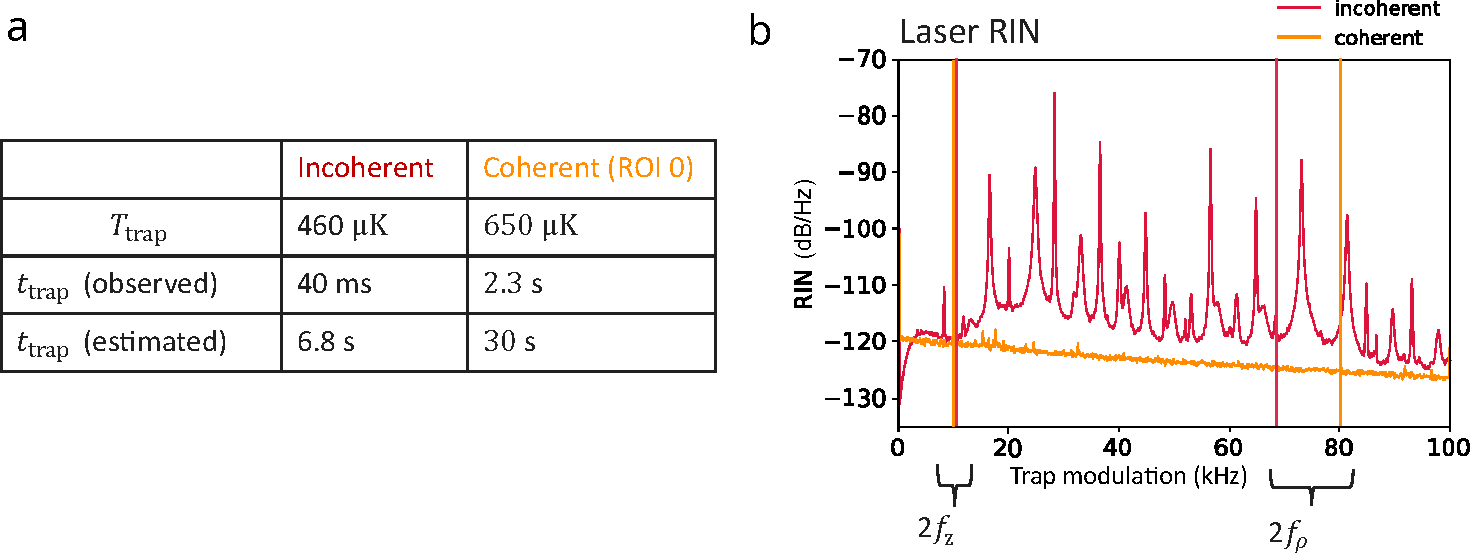
\includegraphics[width=0.9\textwidth]{Images/trap_array_frequencies_and_lifetimes.pdf}
    % {Images/figure9.eps}
    \caption{a) Trap lifetimes and b) RIN spectrum for the incoherent 808 nm laser and coherent 825 nm lasers used for atom trapping. The  atom lifetime in the incoherent trap was measured to be 40 ms, in contrast to a lifetime of at least 5 s measured with the coherent trap. The dashed lines correspond to the twice the measured vibrational frequencies, where the 808 nm RIN level implies a lifetime in excess of 8 s. However, the many large frequency spikes can induce off-resonant heating.}
    \label{fig:rin}
\end{figure}

Quantitatively, we can estimate the RIN-limited lifetime assuming the atom is in a harmonic potential driven at frequency $f$. For a three dimensional potential with radial and axial coordinates $(\rho, z)$, the loss rates and characteristic trap lifetime are given by
\begin{equation}
    \begin{aligned}
    & \Gamma_{\text {trap }, i}=\pi^2 f_i^2 S_k\left(2 f_i\right), i \in\{\rho, z\} \\
    & t_{\text {trap }}=\sum_i \frac{1}{\Gamma_{\text {trap }, i}}
    \end{aligned}
\end{equation}
The calculated lifetimes, given in Fig. \ref{fig:rin}a, are much larger than those observed. For the coherent laser, the observed lifetime is consistent with expectation for a vacuum-limited lifetime. The incoherent lifetime observed is still much shorter than the either the vacuum or RIN-limited lifetimes, but this is likely due to the fact that the atom is driven not only by the RIN frequencies which are on resonant but also by the other components. A more accurate estimate would therefore involve integrating over the full RIN spectrum.

\subsection{Fluorescence imaging}\label{sub:imaging}
The fluorescence images of trapped atoms were captured on a  Hamamatsu C9100-13 EMCCD with 100 ms exposure time. The imaging light was 852 nm, red detuned from the D2 line cooling transition $F=4 \leftrightarrow F'=5$ by about 9 times the natural linewidth, with an intensity around three times the saturation intensity. The single shot image of trapped atoms in Fig. 2a is divided by the average background for the stack of 300 shots taken for that data to account for an uneven intensity pattern on the shots due to a gain variation on the EMCCD sensor itself. The large image was processed with independent component analysis, which has the effect of de-blurring the trapped atoms. However, due to the size of the image (512 by 512 pixels), this process was only effective when the image was broken into smaller chunks. Ultimately, 25 sub-regions in the image stack were processed, and the the summed projected images were stitched back together. The result exhibited a uniform background in each sub-image, with a slight variation between the background level in adjacent sub-regions. Hence, for visual purposes only, the resulting image was plotted with the pixels valued less than 20$\%$ of the maximum intensity clipped.

\section{Two-species trap array}

%To-do 

A dual species trap array consisting of interleaved lattices of intensity minima and maxima can be created with a single wavelength plus transmission mask and 4$f$ filtering as described in Sec. \ref{sec:theory}. A prototypical demonstration of the creation of such a patterned light field was done using a mask fabricated by the Kats group in the ECE department at UW-Madison. The experimentally observed trap profiles, formed with the incoherent laser mentioned above, are shown in Fig \ref{fig:dual_species_traps}. More data and information may be available in the future theses of Sam Norrell and Chengyu Fang, as well (Infleqtion ?? paper, in preparation).

\begin{figure}
    \centering
    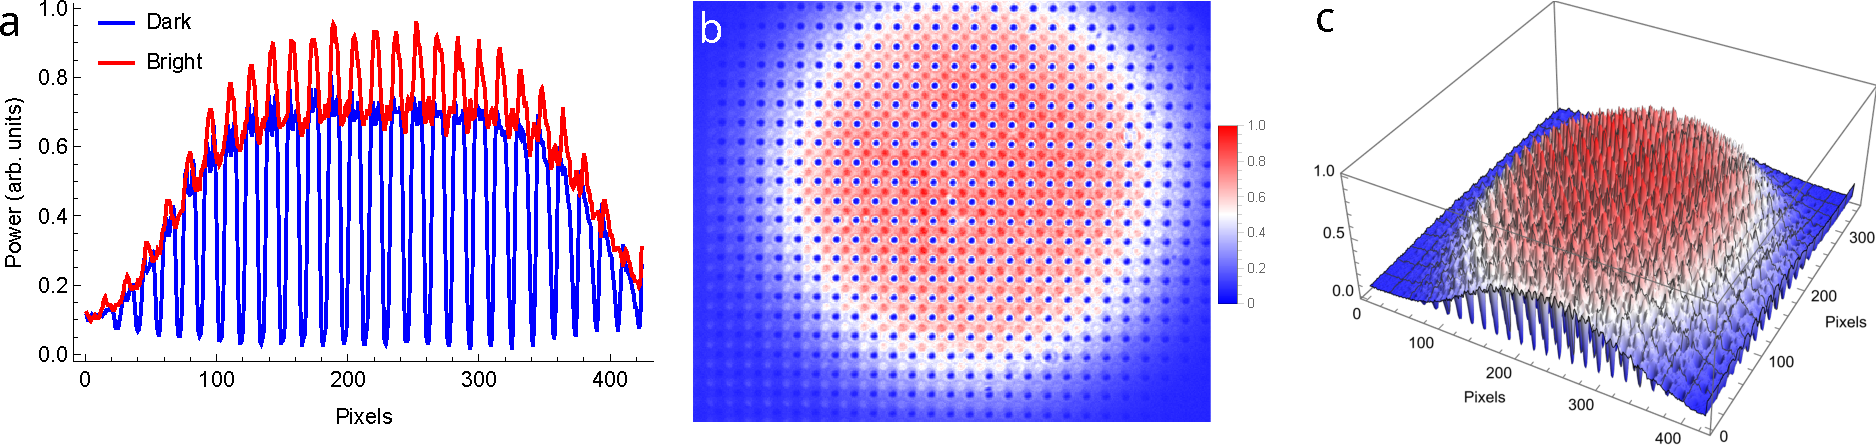
\includegraphics[width=\textwidth]{Images/first_dual_species_trap_image.pdf}
    \caption{An intensity pattern formed by 808 nm incoherent light incident using a prototypical amplitude mask for creating bright and dark traps. The data is shown three ways, increasing in representation dimensionality from \textbf{a} to \textbf{c}. \textbf{a} shows a single pixel row slice of dark traps and one of bright traps, where it can be seen that the depth of both trap kinds are with respect to approximately the same background intensity. The image was taken with the same optical setup used for producing the single-species traps described earlier. The amplitude mask was fabricated by Chengyu Fang of the Kats group in the UW-Madison ECE department.}
    \label{fig:dual_species_traps}
\end{figure}

\section{Vacuum Pressure from MOT loading rate}

The observed short lifetime of atoms in the incoherent trap implied at least one of a few plausible loss mechanisms, including RIN on the trapping laser and loss from collisions with hot background atoms. Because our initial RIN measurements did not seem to fully account for the observed trap lifetime, we measured the vacuum pressure in the science region. 

Often, the pressure of a vacuum system for cold atom experiments is estimated from the reading given by an ion pump current measurement, which gives a lower bound on the pressure seen by the atoms. However, in the case of the experiments above, the ion pump controller reported an implausible measured pressure of $\sim 10^{-4}$ Torr, likely due to leakage current from excessive build up of Cs between the electrodes. The apparatus used for the array trap experiment described above used a ColdQuanta two-chamber vacuum system from a previous iteration of the Cs Atom Qubit Array (AQuA) experiment \cite{Graham2018}. Because the ion pump was not able to be replaced on this system and it was impractical to bake the alkali out of the pump, we used the MOT loading rate to measure the vacuum pressure in the upper science chamber.  

The apparatus used a  dispenser to inject Cs atoms into the lower chamber, from which a 2D MOT could be formed to load a 3D MOT in the upper chamber. However, in the preliminary experiments for this work, forming a 2D MOT was bypassed by running the dispenser long enough to be able to load a 3D MOT directly from the background in the upper chamber. The 2D MOT was in use for all of the work described above, but enough Cs background remained in the upper chamber to allow direct loading of a weak 3D MOT. This turned out to be serendipitous for measuring the background pressure, as described below. 

The number of atoms loaded into the MOT as a function of time is given by
\begin{equation}\label{eq:atomnum}
N(t)=N_s\left[1-\exp \left(-t / \tau_L\right)\right]
\end{equation}
where $N_{\text s}=R \tau_{\text L}=\alpha P_{\text Cs} \tau_{\text L}$ is the saturation atom number, $\alpha$ is the MOT loading cross section, $P_{\text Cs}$ is the Cs partial pressure, $\tau_{\text L}$ is the loading time. The loading time depends on the pressure due to Cs as well as the non-Cs species present and is given by
\begin{equation}
\tau_L=\frac{1}{\beta P_{\text Cs}+\gamma_{\text b}}
\end{equation}
where the terms in the denominator are the sum of collisional loss rates due to Cs and non-Cs species, respectively \cite{RRCAT2020}. Using this, we can re-write the atom saturation number as 
\begin{equation}
N_s=\frac{\alpha}{\beta}\left(1-\gamma_{\text b} \tau_{\text L}\right).
\end{equation}
From literature, $\beta=4.013\times10^7 ~\text{Torr}^{-1} \text{s}^{-1}$ and $\gamma_{\text b}/P=4.9\times10^7 ~\text{Torr}^{-1} \text{s}^{-1}$ \cite{Arnthorp2012}. Fitting Eq. \ref{eq:atomnum} of the background Cs pressure then allows us to extract the ratio $\alpha/\beta$ and $\tau_{\text L}$ which in turn give us the pressures of interest, 
\begin{equation}\label{eq:background_pressures}
\begin{aligned}
    P_{\text {Cs}} &= \frac{N_{\text s}}{\beta \tau_{\text L}}\left(\frac{\beta}{\alpha}\right)_{\text {fit}}\\
    P_{\text {non-Cs}} &= \frac{P}{\gamma_{\text b}}(\gamma_{\text b})_{\text{fit}}
\end{aligned}
\end{equation}
To get $N_s$ as a function of loading time $\tau_{\text L}$, we record need at least two measurement at different values of the Cs background pressure. In single chamber systems, the background pressure can be varied using the dispenser current. The measured MOT fluorescence recorded after waiting increasingly longer $t$ after the MOT beams are turned on gives a curve proportional to Eq. \ref{eq:atomnum}. We effectively varied the Cs background pressure by loading the 3D MOT with and without the 2D MOT on, from which we obtained a Cs background pressure of $1.86\times10^{-8} ~\text{Torr}$ and non-Cs pressure of $8.11\times10^{-9} ~\text{Torr}$ using Eqs.  \ref{eq:background_pressures} above. The loading curves are shown in Fig. \ref{fig:CsMOT_loading}.

\begin{figure}
    \centering
    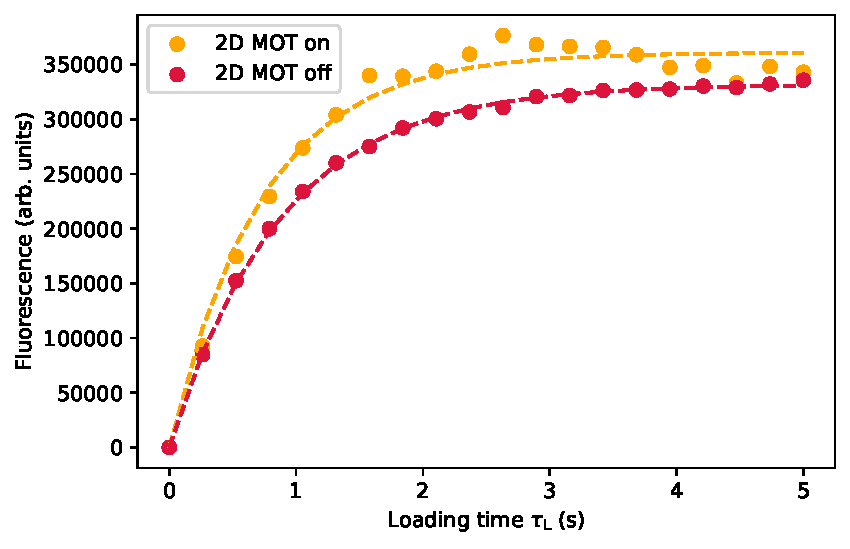
\includegraphics[width=0.6\textwidth]{Images/CsMOT_loading_curves.pdf}
    \caption{Loading curves for the Cs 3D MOT, with and without the 2D MOT on. In the latter case the 3D MOT is loaded directly from background. The fits to Eq. \ref{eq:atomnum}, where fluorescence is used as a proxy for $N_{\text s}$, give $N_{\text s},\tau_{\text L}=(360821.457,0.727)~\text{and}~(331722.200,0.872)$. Fitting a line to these pairs gives $\alpha/\beta=5.076\times10^5$ and $\gamma_{\text b}=0.397 ~\text{s}^{-1}$ from which the pressures given in the text are obtained using Eq. \ref{eq:background_pressures}.}
    \label{fig:CsMOT_loading}
\end{figure}

These pressures seem realistic and imply collision-limited dipole trap lifetimes on the order of several seconds, consistent with those measured for the coherent laser.

% \end{document}
%
% ****** End of file apssamp.tex ******

% \include{intro/intro}
% \include{motivation/motivation}
% \include{related/related}

%% etc, etc.

%% Do you have appendices?  If so, add them here, just like chapters.
\begin{appendices}
\part{Appendix}\label{part:appendices}
\chapter{GOOD Logger}\label{ch:template}

The GOOD Logger is a Python program which can be configured to read from a variety of hardware in the lab and post the data to the lab's Origin server. Origin is a program written by Matt Ebert which allows posting to and subscribing to streams or channels of data written to a SQL database. Before the GOOD logger, where GOOD stands for Get Origin Our Data, there were only single-purpose servers in the lab for posting data to origin. The GOOD Logger filled this void by providing a straightforward means to log data from several instruments in the lab in parallel, with a single server. 

In its infancy, the GOOD Logger existed in the Hybrid lab, written by Juan Bohorquez to read from some particular instruments. The author of this work, in collaboration with Juan, extended the functionality of the Hybrid logging code to abstract away the details of instrument hardware and reduce the upfront work of the user to entering some parameters in two config files. 

The primary motivation for the GOOD Logger arose when  transient events in the Rb lab \footnote{Before the network project existed} were resulted in sudden loss of the MOT or reduction of atom loading rate during an experiment. The ability to monitor and log signals from multiple sources in a lab asynchronously is of tremendous value for identifying this type of issue. In the case mentioned, we were able to find that some of the homebuilt current drivers for the MOT coils were faulty and exhibited sudden jumps in the current output, shown in Fig. \ref{fig:coiljumps}.

\begin{figure}[!ht]
    \centering
    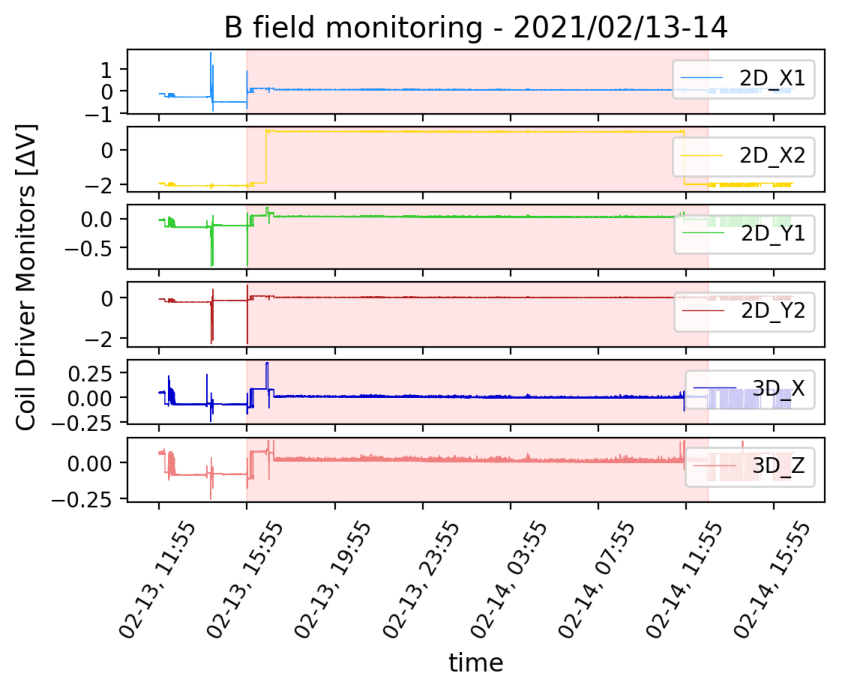
\includegraphics[width=0.9\textwidth]{Images/goodlogger_coil_jumps_20210213_14.pdf}
    \caption{Coil driver current monitor outputs, for selected 2D and 3D MOT coils measured with an NI DAQ analog input card and logged using the GOOD Logger. The shaded red region is where experiments are not being run, which shows that abrupt changes occur in the coil values came about without influence by the experimenters.}
    \label{fig:coiljumps}
\end{figure}

Since the publication of \cite{Bohorquez2023}, the GOOD Logger has been adapted to allow writing data to a local database using PostgreSQL. This is advantageous in terms of speed when reading from the database, and allows for seamless use of freely available data visualization servers such as Grafana. The ease of this solution stands in contrast to the many attempts at custom plotting solutions there have been in the group in order to cooperate effectively with the Origin server. To-date, the network lab uses the GOOD Logger for monitoring the four Gamma Ion pumps for the two nodes, two open-loop thermocouples in the temperature controlled experiment box (interfaced with a Measurement Computing USB-TEMP device), a Stefan-Meyer 3-axis magnetometer, and various Sinara Zotino channels and coil monitors as needed.



% the hierarchy is 
% chapter,section,subsection,etc
% \end{doublespacing}

\chapter{Temperature-controlled experiment box}\label{ch:experiment_box}

Having an environment with a stable temperature is crucial for many optics experiments, as it reduces thermal expansion or contraction leading to drift in optical alignment as well strain changes in non-PM single mode optical fibers resulting in polarization state drift. For the network experiment, most of the optics for launching beams at the atoms are glued inside the vacuum chamber, but the external MOT beams and myriad of optical fibers are still susceptible to thermal drift. To mitigate this, both nodes live in a table-top enclosure with a temperature control loop. 

The enclosure or "experiment box" (Fig. \ref{fig:experiment_box_frame}) is constructed with a frame made from 1" x 0.5" 8020 bars and removeable panels made from 0.25" Alumalite plus a layer of microwave-damping foam (Laird ECCOSORB® QR-13AF) on the inner side of the panels held in place by flameless flame retardant paper (Pacon). The paper prevents degraded foam particles from dropping onto the optics while mitigating risk of a laser-induced fire. The panels also include sections with electrical feedthroughs including BNC, SMA, USB, XLR, and ethernet. The overall design of the box was based on the one described in \cite{kwon2019rydberg}, with some minor modifications from Arian Noori and Ethan Lu.

\begin{figure}[!ht]
    \centering
    \includegraphics[width=1\textwidth]{Images/chiller_TEC_control_diagram.pdf}
    \caption{Chiller, TEC, and TEC controller connections. Courtesy Arian Noori.}
    \label{fig:box_TEC_control}
\end{figure}

A temperature control loop, shown schematically in Fig. \ref{fig:box_TEC_control} is used to keep the air inside the box stable within about 0.1 $^{\circ}$C (typical). Six thermoelectric cooler (TEC) units (Laird TEC LA-075-24-02) with fans are placed around the base of the box in order to exchange heat between the air in the box and chilled water. The water is chilled and pumped through the closed loop by a LabTech Smart H150-1000 water chiller. Heat flow mediated by the TECs is regulated by PI loops implemented with one Wavelength electronics PTC5K-CH TEC controller per TEC, where each controller reads the value of a 10k thermistor placed in the air near the TEC for that channel Fortuitously, the TEC controllers are analog, and therefore do not radiate magnetic noise from pulse-width modulation which can contribute to qubit decoherence. Some mechanical design details are shown in Figs. \ref{fig:box_TEC_mount_side} and \ref{fig:box_TEC_mount_back}.

\newpage

\begin{sidewaysfigure}[!ht]
    \centering
    \includegraphics[width=1\textwidth]{Images/network_box_TEC_mount_sides.pdf}
    \caption{Mounting plate for TECs on sides of box. Courtesy Arian Noori.}
    \label{fig:box_TEC_mount_side}
\end{sidewaysfigure}

\newpage

\begin{sidewaysfigure}[!ht]
    \centering
    \includegraphics[width=1\textwidth]{Images/network_box_TEC_mount_back.pdf}
    \caption{Mounting plate for TECs on back of box. Courtesy Arian Noori.}
    \label{fig:box_TEC_mount_back}
\end{sidewaysfigure}

\newpage
% Remember to insert \end{doublespacing} somewhere after this... not necessarily in the same .text file though
% \begin{doublespacing}

% \part{ Appendix}\label{part:appendices}
\chapter{Mechanical drawings}\label{ch:mech_drawings}

This appendix contains reproductions of mechanical drawings for some key components of the apparatus(es) described in this thesis.

\newpage

\begin{sidewaysfigure}[!t]
    \centering
    \includegraphics[width=1\textwidth]{Images/mdc_chamber_20220428.pdf}
    \caption{Mechanical drawing of the ultra-high vacuum science chamber from MDC Precision. The annotations in red were added to the original drawing provided by MDC to determine previously unspecified dimensions}.
    \label{fig:drawing_mdc_chamber}
\end{sidewaysfigure}

\newpage

\begin{sidewaysfigure}[!ht]
    \centering
    \includegraphics[width=1\textwidth]{Images/AQX Networking Box Frame LAYOUT.pdf}
    \caption{CAD drawing of the experiment box courtesy of Price Engineering. The slots in the top and back panels are for attaching cable feedthrough panels.}
    \label{fig:experiment_box_frame}
\end{sidewaysfigure}

% \begin{sidewaysfigure}[!t]
%     \centering
%     \includegraphics[width=1\textwidth]{Images/fig_coming_soon.png}
%     \caption{Mechanical drawing of the MACOR substrate or ``bridge" for the parabolic mirror version of the experiment design}.
%     \label{fig:macor_bridge_mirror}
% \end{sidewaysfigure}

\newpage

\begin{sidewaysfigure}[!t]
    \centering
    \includegraphics[width=1\textwidth]{Images/nipro_parabolic_mirror_drawing.pdf}
    \caption{Mechanical drawing of the parabolic mirror used as the focusing optic for both the dipole trap and photon collection in a quantum network node. The mirror was coated with a layer of nickel and then protected silver}.
    \label{fig:mirror}
\end{sidewaysfigure}

\begin{sidewaysfigure}[!ht]
    \centering
    \includegraphics[width=1\textwidth]{Images/recessed_window_draft.pdf}
    \caption{Draft of the specifications for the custom recessed windows for the cavity node. The remaining specifications are given in Fig. \ref{fig:recessedwindowdrawing}}
    \label{fig:recessedwindowdraft}
\end{sidewaysfigure}

\begin{sidewaysfigure}[!ht]
    \centering
    \includegraphics[width=1\textwidth]{Images/recessed_viewport_for_kimball_6in_spherical_octagon.pdf}
    \caption{CAD drawing of the custom recessed windows for the cavity node. The remaining specifications are given in Fig. \ref{fig:recessedwindowdraft}}
    \label{fig:recessedwindowdrawing}
\end{sidewaysfigure}

% \part{Template}\label{part:appendices}
\chapter{Network node ingredient lists}\label{ch:ingredients}

% the hierarchy is 
% chapter,section,subsection,etc

% todo: put the ingredient list pdf(s) here. they are on the wiki but need updating. I think the powerpoint lives on the Coffee lab PC but i may have slacked it to myself.

Below, there are ``ingredient lists" for key sections of the network experiment apparatus, including the optical chip.

\newpage

\begin{sidewaysfigure}[!t]
    \centering
    \includegraphics[width=1\textwidth]{Images/optical_chip_parts_mirror_version_20230316.pdf}
    \caption{An ingredients list for the parabolic mirror version of the optical chip which was used in the first network node. The columns labeled ``have?" are so that this sheet can be used to take inventory of the parts we have on hand. In the upper right, the parabolic mirror tube is drawn as being transparent only for the purpose of making the internal contents visible.}.
    \label{fig:drawing_mdc_chamber}
\end{sidewaysfigure}

\newpage
% \part{Template}\label{part:appendices}
\chapter{A Cavity-based network design}\label{ch:cavitynode}

In light of the analysis in \cite{Young2022}, we had planned to implement a cavity version of the network experiment. One of the main bottlenecks in the remote entanglement generation rate for a quantum network is the photon collection efficiency, which can approach unity by placing the communication qubits in a suitable optical cavity. By using a cavity operated in the near-concentric regime, i.e. with length $L$ just below twice the mirror radii of curvature $R$, a small mode waist can be obtained while maintaining a relatively large mirror separation. This means that we acheive a strong interaction between the an atom and the cavity mode while avoiding deleterious effects associated with short cavities such as the accumulation surface charges which can induce significant Stark shifts on Rydberg states \cite{Bohorquez2023}. Moroever, the cavity length allows for increased optical access, allowing, e.g., for forming a MOT within the cavity. This appendix presents the mechanical and optical design for cavity-based network node, for which all of the main parts have been ordered. The project is on-pause as of the time of this writing, as the lab pivots toward dual-species remote entanglement.

\section{Cavity Mirrors}\label{sec:cavmirrors}

The cavities were designed to simultaneously support modes at 780 nm and 1540 nm, the wavelengths of the emitted photons for networking and cavity lock reference, respectively. Depending on the choice of phases imparted by the mirror coatings, the nodes and anti-nodes of standing waves at these two wavelengths can line up in different ways, as is described in \cite{garcia2020overlapping}. By suitable choice of these phases, the 1540 field can be used to provide tight axial confinement of atoms within the pancakes shaped high intensity regions formed by antinodes in the standing wave. The analysis to calculate the mirror coating phases was done by Akbar Safari.

\begin{figure}[!ht]
    \centering
    \includegraphics[width=0.9\textwidth]{Images/cavity_mirror_substrate.pdf}
    \caption{The fused silica cavity mirror substrate design and photos of the final product from Optics Technology in Rochester, NY. The chamfered edges allow clearance for $\sim1$ mm diameter MOT beams to be sent through the cavity. Design image and photos courtesy of Akbar Safari.}
    \label{fig:cavmirror_substrate}
\end{figure}

The cavity is designed to be ``one-sided" at 780 nm, such that nearly all of the photons emitted from the atom exit through only one of the two mirrors. The 1540 nm laser used for the cavity lock will be coupled into the cavity through the other mirror. 

\section{Mode Matching}\label{sec:cavmatching}

Mode matching light to a near-concentric cavity involves converting an incident plane wave (i.e. a collimated beam) into a spherical wave which focuses down to the cavity waist, which is accomplished optimally by using a cavity mirror whose back surface is elliptical \cite{Durak_2014}. However, for ease of budget and design complexity, we can approximate such a monolithic mirror substrate with by a flat-back cavity mirror and a plano-convex lens, placed nearly back to back (Fig. (\ref{fig:modematchapprox})). 

\begin{figure}[!ht]
    \centering
    \includegraphics[width=0.9\textwidth]{Images/mode_matching_mirror_approximation.pdf}
    \caption{A cavity mirror with an elliptical back surface (right) for transforming a spherical wave in the cavity to a plane wave outside the cavity can be approximated by a mirror with a flat back plus a plano-convex spherical lens (left). The spherical surface of the lens should have the same curvature constant as the elliptical surface. See text for details.}
    \label{fig:modematchapprox}
\end{figure}

The curvature of optical surface, or sag, for a conic surface $i$ ($i=1$ is the mirror surface, $i=2$ is the back surface) is given by 
\begin{equation}\label{eq:sag}
    sag_i(r) = \frac{c_i r^2}{1+\sqrt{1 - (1+k) c_i^2 r^2}} 
\end{equation}
where $c$, $k$, and $r$ are the curvature, conic constant, and radius from the optical axis. For the desired elliptical surface, we have $c=a/b^2$ and $k=(b^2-a^2)/a^2$ in which $b=f \sqrt{(n-1)/(n+1)}$, $a = f n/(n+1)$, where $n$ is the index of refraction of the mirror substrate and $f$ its effective focal length. Taylor expanding Eq. (\ref{eq:sag}) gives
\begin{equation}
    \frac{c r^2}{2} + \frac{c^3 r^4}{8} + \frac{k c^3 r^4}{8} + \mathcal{O}(r^5).
\end{equation}
For $f=10 mm$, $n=1.765$ (Fused Silica at 780 nm), and $r=0.5 mm$ (clear aperture), a spherical surface ($k=0$) deviates from a spherical one on the order of $10^{-4}$, justifying our approximation.

We want to solve for parameters for two lenses, one to approximate the role of an elliptical surface for mode-matching to the cavity, and one for coupling to match the collimated cavity output to a fiber.

For a given desired cavity mode waist $w_0$ at wavelength $\lambda$; and mirror substrate $n$ and thickness $t$ (if monolothic mirror $+$ elliptical surface) and clear aperture $r_{CA}$,  we can compute the effective focal length $f$. Note that $t$ is chosen to be the thickness of the flat-back mirror substrate plus some additional thickness to account for that of the lens we will use to approximate the elliptical surface. We then solve the following two equations:
\begin{align} 
    t_c &= t - sag_1(r_{CA}) \\ 
    f &= t_c + 1/c_1  
\end{align}
with $c_1$ equal to the reciprocal of the mirror radius of curvature and $t_c$ is the total center thickness.

The effective focal length of a lens with thickness $d$ is given by
\begin{equation}
    efl = \frac{1}{(n-1)(c_1 - c_2 + \frac{c_1 c_2 (n-1)d}{n})}
\end{equation}
where $c_1=0$ for a plano-convex lens. To approximate an elliptical surface, we want the spherical side have to R.o.C. of $ -1/c_2 = b^2/a$, which depends on $f$ which can be solved for as shown above.

The required fiber coupling lens focal length is found by using the waist transformation for Gaussian beams, starting with the cavity waist. The waist on the back surface of the monolithic mirror is
\begin{equation}
    w_1 = \frac{\lambda f}{w_0 \pi}
\end{equation}
and the required fiber coupling lens focal length is
\begin{equation}
    f_c = \frac{\pi w_1 w_{\textrm{fiber}}}{\lambda}.
\end{equation}

Mathematica code for this procedure of calculating mode matching lenses is available upon request. This procedure was used for picking candidate off-the-shelf lenses, which were then checked in Zemax with a model of the flat-backed mirror substrate for fiber coupling and mode matching efficiency at the design wavelengths. 

Lenses were chosen for a cavity waist of $8~\mu $m at 780 nm, correpsonding to a cavity length which deviates from near-concentric by $67.5~\mu \mathrm{m}$ (i.e. the critical distance) and with fused silica mirror substrates with 6 mm thickness, and mirror RoC 2 mm and clear aperture 0.5 mm (Fig. \ref{fig:cavmirror_substrate}). Simulations in Zemax using Physical Optics Propagation were done to compute the fiber coupling efficiency for the 780 nm mode emitted by the cavity and mode-matching efficiency for 1560 nm light launched from a SM fiber, where the results are tabulated in Fig. \ref{fig:modematchdesign}. The spacings between lenses were optimized for the best efficiencies. For the same set of lenses and spacings, the calculations were repeated for two different 780 nm waist values (corresponding to different cavity lengths in the simulation) to see how forgiving the design is at cavity lengths which are increasingly more stable.

\begin{figure}[!ht]
    \centering
    \includegraphics[width=0.9\textwidth]{Images/zemax_cavity_design.pdf}
    \caption{Mode matching lenses for coupling a 1560 nm beam from a SM fiber into the cavity, and a cavity mode at 780 nm out of the cavity and into an SM fiber. The lenses are, from left to right, \href{https://www.edmundoptics.com/p/043-na-450mm-fl-1050-1600nm-ar-coated-molded-aspheric-lens/26661/}{Edmund 83-580}, \href{https://www.edmundoptics.com/p/40mm-dia-x-60mm-fl-nir-ii-coated-plano-convex-lens/21908/}{Edmund 67-447}, \href{https://www.edmundoptics.com/p/50mm-diameter-x-75mm-fl-785nm-v-coat-pcx-lens/31486/}{Edmund 89-014}, and \href{https://www.thorlabs.com/thorproduct.cfm?partnumber=355660-B}{Thorlabs 355660-B}. Hyperlinks to products are available online.}
    \label{fig:modematchdesign}
\end{figure}

\section{Cavity opto-mechanics}\label{sec:cavopto}

The mechanical design of the cavity uses Macor housings to secure the cavity mirror substrates, mode-matching lenses, fiber coupling lenses, and ferrules for optical fibers. The fiber coupling lenses and fiber ferrule are held in a separate housing from the mode-matching lens and cavity mirror to allow for relative alignment tuning or the option to forego a fiber-coupled cavity in favor of free space mode-matching on either or both sides of the cavity. This design is shown for both cavity sides in Fig. \ref{fig:modematchhousings} for the optics in Fig. \ref{fig:modematchdesign}.

\begin{figure}[!ht]
    \centering
    \includegraphics[width=0.9\textwidth]{Images/mode_matching_housings.pdf}
    \caption{Solidworks models of the housings designed to mount the fiber and cavity mode matching optics to the cavity mirrors for both the 780 nm photon collection side (b) and the 1560 nm locking side (a). The housings are designed to be Macor and are vented for use in vacuum. Note: the models shown were modified after the above images were made to include a chamfer on the cavity mirror end of each housing to match the cavity mirror's own chamfer, in order to not clip MOT beams. This update can be seen in Fig. \ref{fig:cavitybridge}.}
    \label{fig:modematchhousings}
\end{figure}

The entire cavity assembly can be mounted in Macor V-groove pieces which themselves are mounted on a linear alignment piece or "bridge" which holds the entire cavity together once the individual optic housing and V-grooves have been aligned and glued. The cavity mirror housing V-grooves are in turn mounted to shear-mode piezo-electric transducers (Noliac NAC2402-H3.4). The exact height of the cavity mirror may need to be adjusted, which can be done by shimming the V-grooves on one side of the cavity. For this purpose, titanium shims (Surepure Chemetals) were ordered, as titanium and Macor have very similar coefficents of thermal expansion, which maintain their similar values and, crucially, the same sign over the range of temperatures including our vacuum bakeout. This design is shown in Fig. \ref{fig:cavitybridge} with an alternative fiber coupling housing design allowing for the insertion of $45^{\circ}$ mirrors to be inserted if switching to free-space mode-matching is desired. This allows for a plan B if fiber coupling becomes misaligned, for example, while the glue cures.
\begin{figure}[!ht]
    \centering
    \includegraphics[width=0.45\textwidth]{Images/cavitybridge.pdf}
    \caption{Solidworks models of the assembled cavity with optional mirrors inserted between the fiber coupling and mode-matching optics housings on each side, to allow for free-space cavity coupling. The cavity length can be modulated using piezo-electric elements (dark gray). Note that the V-grooves on the left have small dimples to mark that they are 100 $\mu \mathrm{m}$ shorter vertically, to allow for shimming to the correct height.}
    \label{fig:cavitybridge}
\end{figure}

\section{MInt Chip}\label{sec:mintchip}

In light of the difficulty in assembling the chip-based node discussed in Ch. \ref{ch:nodes} and the lack of ability to pivot or course correct in the event of catastrophy (e.g. a part glued down incorrectly), here we present an updated architecture dubbed MInt Chip (Modular Integrated Chip). The MInt Chip systems consistes of Ti substrate with a grid of tapped holes, acting a miniature breadboard to which miniature optomechanical modules can be attached. Components of the MInt Chip system machined from Grade 2 Ti (manufactured by Fast Radius), including hardware for mounting the cavity described in the previous section, is shown in Fig. \ref{fig:mintchip}.
\begin{figure}[htb]
    \centering
    \includegraphics[width=0.7\textwidth]{Images/mint_chip.pdf}
    \caption{a) The titanium MInt Chip substrate and b,(c) cavity mounting hardware.}
    \label{fig:mintchip}
\end{figure}

As a first pass design for the MInt Chip based cavity apparatus, we elected to use free space beams and a chamber with more plentiful optical access compared to the custom chamber used in the network experiment described in this thesis. A SOLIDWORKS model of this apparatus is shown in Fig. \ref{fig:cavnodechamber}. The author elected to use mainly commercially available components, including a commercially available vacuum chamber (Kimball Physics 6" Spherical Octogon) and standard viewports (Accuglass 115063, 780~1064nm Broadband AR Coated Viewport). Custom recessed windows were designed (on order from MDC Precision) to accomodate our broadband custom high NA objective lenses (JenOptik, 0.4 NA).
\begin{figure}[htb]
    \centering
    \includegraphics[width=0.9\textwidth]{Images/mint_chip_science_chamber.pdf}
    \caption{The cavity node vacuum chamber and MInt Chip mounting system. The red sections in (a) represent quadrupole coils and the black object at the bottom represents a 0.4 NA  custom objective, both of which are in the bore of a custom recessed objective.}
    \label{fig:cavnodechamber}
\end{figure}
Mechanical drawings of the recessed windows are given in Figs. (\ref{fig:recessedwindowdrawing}, \ref{fig:recessedwindowdraft}) in Appendix \ref{ch:mech_drawings}.
    



% \part{Template}\label{part:appendices}
\chapter{Two-piezo filter cavity}\label{ch:cavity}

% the hierarchy is 
% chapter,section,subsection,etc

% todo: put the ingredient list pdf(s) here. they are on the wiki but need updating. I think the powerpoint lives on the Coffee lab PC but i may have slacked it to myself.

\section{Optical cavities as spectral filters}

Fabry-Perot optical cavities are convenient tools for spectral filtering of a laser field when one is interested in retaining spectral content only within a certain window centered around the carrier frequency. An example of this situation comes in the context of driving Rydberg transitions for quantum gates, where the gain required for locking the laser creates unwanted "servo bumps" in the spectrum where the sign of the feedback flips, which can cause gate rotation errors \cite{jiang2023sensitivity}. This can be remedied with "filter cavities" which have a linewidth large compared to that of the laser carrier, but narrow enough that the servo bumps are not transmitted \cite{kwon2019rydberg}. The filter cavity, whose length can be modulated using a piezoelectric element attached to one of the mirrors, is then locked to transmit the laser carrier frequency using the PDH locking technique.

One potential issue with using a cavity for filtering is the transfer of cavity length instability to intensity noise on the transmitted light. This length instability can stem from ambient acoustic noise propagating through the cavity, or a deficiency with the PDH lock, such that the cavity length oscillates around the lock point defined by the laser frequency. The former issue can be remedied by placing the optical cavity in a vacuum chamber and using a damping material between the cavity body and chamber. The latter issue depends on the lock parameters such as gain and bandwidth, as well as the sensitivity and bandwidth of the piezo. 

This appendix discusses a cavity intended to improve on intensity noise observed on the original version of filter cavities in this group\cite{Young2022}. The cavity was designed and constructed with great help from Michael Bergdolt, who was an undergraduate student at the time. The cavity described is based on a two-piezo design, and is a modified of the predecessor single-piezo version described in \cite{kwon2019rydberg}. The original cavity design will not be described in detail here, as all of the details not explicitly mentioned were kept the same, from the mechanical design to the mirrors used and the vacuum hardware.

\section{Design principle}

For locking a cavity to a sufficiently narrow-linewidth laser, it is  advantageous to have two piezos\cite{Braverman2018}. One piezo with a sufficiently long range is needed in order to guarantee that the cavity length can be tuned to be resonant with the laser. By analyzing this first requirement, we can motivate the necessity of a second, much less sensitive piezo for locking to a narrow laser. In order to guarantee that the cavity can be brought onto resonance with the laser, we must be able to change the cavity length by one half wavelength, corresponding to one free spectral range (FSR), defined as
\begin{equation}
    FSR = \frac{c}{2L}
\end{equation}

where $c$ is the speed of light and L is the length of the cavity. For the long range or ``slow" piezo, PiezoDrive SR120610, the average sensitivity is 12.857 $V/ \mu$m, meaning that it takes about 5 V to change the cavity length by one FSR at 780 nm. 
For locking the cavity to a narrow linewidth laser for Rydberg, we may want the frequency stability of the lock to be $\sim 100$ Hz. Converting this frequency change $\delta \nu$ to a change in wavelength $\delta \lambda$, given by $|\delta \nu| = \delta\lambda(c/\lambda^2)$, gives $\delta \lambda \sim 2*10^{-19}$ m. Considering that there are $\sim 256000$ half wavelengths in a 10 cm long cavity ($L=m \lambda/2$), the cavity length must be stabilized to $2.6*10^{-14}$ m. Given the sensitivity of the PiezoDrive SR120610, we would need a piezo driver with noise $\ll 0.3~\mu$V, which is usually unrealistic.

A much less sensitive piezo can be used to overcome this requirement on the piezo driver noise. The Boston Piezo-Optics PZT-5H, chosen for this purpose, has an average sensitivity of 1709 $V/\mu$m. The constraint on the voltage noise is now $44 \mu$V, which is feasible with commercially available drivers (e.g. the PiezoDrive PDU150). By contrast, to scan one FSR with this piezo would require 666 V, over three times the range of typical commercially available piezo drivers. Hence, the need for two piezos is apparent. 

\section{Cavity construction}

The two-piezo cavity construction differs from the original build in that the additional slim piezo is mounted between the long range piezo stack and the mirror. Unlike the long piezo, which comes with wires attached to electrodes opposite sides of the cylindrical surface, the slim piezo's electrical contacts are gold-plated end faces, and electrodes do not come pre-attached. Because of this, it was necessary to design mounting hardware which would not completely obscure the end faces, and would leave clearance for attached wires. The result is shown 

\begin{figure}[!ht]
    \centering
    \includegraphics[width=0.9\textwidth]{Images/two_piezo_stack_assembly.pdf}
    \caption{Assembly stages of the two piezo stack for the filter cavity. a) Fast piezo holder glued atop slow piezo, which is glued to the invar cavity spacer. b) Fast piezo with soldered connections glued into its holder, with glue applied for the next spacer. c) Spacer applied to fast piezo, which gives clearance for the positive electrode. d) The assembly is glued using a makeshift clamp made with acrylic panels, which keep the components sufficiently parallel while the glue cures.}
    \label{fig:cavity_fig1}
\end{figure}
% \part{Template}\label{part:appendices}
\chapter{Collective radiance in atomic arrays and volumes}\label{ch:collectiveradiance}

As originally explored by Dicke, two or more spins in proximity to each other will have their spontaneous emission rate modified due to interference\cite{Dicke1954}. His original thought experiment is presented in Fig. (\ref{fig:DickeNeutronDecay}) Such collective interactions can either enhance or suppress the spontaneous decay rate of many quantum emitters, compared to any individual emitter in isolation, depending on the spacing between the emitters as a fraction of the emission wavelength. In addtion to modified decay rates (or equivalently, excited state lifetimes), the emission pattern may be highly directional\cite{ballantine2020subradiance}, and the light even from a disordered ensemble of atoms may be exhibit spatial coherence \cite{gold2022spatial}. These emergent phenomena are of interest for many-body physics studies as well as potential applications in quantum technologies, such as for creating an "atomic antenna", efficiently mapping light into an optical fiber e.g. for quantum communication \cite{grankin2018free, jones2020collectively}.

\begin{figure}[!ht]
    \centering
    \includegraphics[width=0.9\textwidth]{Images/Dicke_neutron_decay.pdf}
    \caption{A pictorial representation of Dicke's simple explanation for the existence modified spontaneous decay rates using neutrons. In the case where two neutrons are far apart, their decay rates are unchanged and the probability to observe emission if one neutron is excited is unity if we wait long enough. For the case where the neutrons are sufficiently clsoe together, the state is now a superposition of a singlet and triplet state, and the emission probability is $1/2$.}
    \label{fig:DickeNeutronDecay}
\end{figure}

In what follows, we will give an overview of the physics of collective radiance effects in ordered arrays through a numerical study of the conditions in which they arise. We will also explore to what extent the interesting emergent features are sensitive to various imperfections in the atomic arrays. Numerous studies have been done to calculate various features of interest for different geometries \cite{moreno2019subradiance, ballantine2020subradiance, bettles2016enhanced} which may provide more detailed analysis than what is outlined here.

\section{Hamiltonian for the single-excitation subspace}

For two level atoms arranged in a 2D grid (Fig. (\ref{fig:2datomgrid})) interacting with an incident oscillating electric field near the tranisiton resonance, it is straightforward to write down the semi-classical system Hamiltonian. We will limit this analysis to the single-excitation subspace, meaning that the Hilbert space is truncated so there is at most one excitation $\hbar \omega_0$ in the array, where $\omega_0$ is the atomic transition angular frequency. 

\begin{figure}[!ht]
    \centering
    \includegraphics[width=0.45\textwidth]{Images/atomgrid.pdf}
    \caption{A 2D grid of two-level atoms, or equivalently, classical electric dipoles.}
    \label{fig:2datomgrid}
\end{figure}

The matrix elements of the effective dissipative Hamiltonian are given by
\begin{equation}\label{eq:greenham}
    \bra{1_i} H \ket{1_j} = H_{ij} = \Omega_{ij}(1 - \delta_{ij}) + i\gamma_{ij}\delta_{ij}
\end{equation}
where $\Omega_{ij}$ and $\gamma_{ij}$ are related to the Green's tensor and the states $\ket{1_i}$ are a shorthand for the state with only atom $i$ excited: 
\begin{equation}
    \ket{1_i} = \ket{0_0} \otimes \ket{0_1} \otimes ... \ket{1_i} ... \ket{0_{N-1}} \otimes \ket{0_N}
\end{equation}

The effective coupling and decay terms are given by the dipole-dipole interaction between radiating dipoles with orientations $e_{\mu}$ and $e_{\mu}$ for dipoles (atoms) at positions $r_i$ and $r_j$: 
\begin{equation}
    \Omega_{ij} + i \gamma_{ij} = \frac{6\pi \gamma}{k^3}\hat{e_{\mu}}\cdot G(\mathbf{r}_i - \mathbf{r}_j) \cdot \hat{e_{\nu}}
\end{equation}
where $G$ is the Green's tensor, giving
\begin{equation}
    \begin{aligned}
        G\left(\mathbf{r}\right) \cdot \hat{e}_{\nu}= & \frac{e^{i k r}}{4 \pi r}\left[(\hat{\mathbf{r}} \times \hat{e}_{\nu}) \times \hat{\mathbf{r}} \right. \\
        & \left.+\left(\frac{1}{k^2 r^2}-\frac{i}{k r}\right)\left(3 \hat{\mathbf{r}}(\hat{\mathbf{r}} \cdot \hat{e}_{\nu})-\hat{e}_{\nu}\right)\right]
    \end{aligned}
\end{equation}
where $k$ is the wavenumber. We can now investigate dynamics of such a system by numerically, including finding the eigenmodes by diagonalizing the Hamiltonian for various system geometries, as well as solving for temporal dynamics given an initial excitation in the array.

\section{Eigenmodes, decay, and emission patterns of 2D arrays}
For a square grid of atoms we can numerically diagonalize Eq. (\ref{eq:greenham}) to find the eigenvalues $\lambda_n$ where the collective Lamb shift $\delta_n$ and decay rate (linewidth) $\nu_n$ of the mode are given by the real and imaginary parts, respectively, of $\lambda_n$. For the dipole orientations we will restrict the system to a few different cases, all of which have $|e_{\mu}| = |e_{\nu}|$ and polarization aligned either perpendicular to or parallel with the plane in which the atoms live. For the perpendicular case, we will label the case of all dipole moments aligned as "symmetric", and "anti-symmetric" for the case where each dipole is $\pi$ out of phase with its neighbor (Fig. (\ref{fig:symm_antisymm_modes}))

\begin{figure}[!ht]
    \centering
    \includegraphics[width=0.9\textwidth]{Images/symm_anti_symm_modes.pdf}
    \caption{Symmetric (a) and anti-symmetric (b) modes of an 11x11 square grid of atoms with out-of-plane polarization, found by sorting the eigenmodes by maximum overlap with the state of interest.}
    \label{fig:symm_antisymm_modes}
\end{figure}

The linewidths for the symmetric states vary as a function of array spacing, where the suppression and enhancement compared to the natural linewidth can be thought of as a sort of two-dimensional cavity, where modulating the length in each direction brings the system into and out of resonance. Indeed, placing a single atom in a 1D cavity is directly analagous to placing it in a periodic array of atoms, where loosely speaking, a higher finesse cavity would correspond to an array with more atoms. The linewidths versus array spacing for different polarization orientations is shown in Fig. (\ref{fig:collective_linewidths_2d}), where the red circle emphasizes that four orders of magnitude linewidth suppression can be acheived with just 25 atoms. It is clear that for in-plane polarization the linewidth is close to or enhanced compared to natural linewidth, whereas there can be significant supression for polarization perpendicular to the plane. An intuitive explanation of this is arrived at by considering that the emission of linearly polarized radiation will propagate perpendicularly to the orientation of the dipole. Thus, for polarization perpendicular (parallel) to the atomic array, the radiation will propagate mostly in the (perpendicular to) plane of the array.

\begin{figure}[!ht]
    \centering
    \includegraphics[width=0.9\textwidth]{Images/collective_linewidths_2d.pdf}
    \caption{Linewidths for various polarization orientations of atom arrays of two sizes. For the 31x31 array, the author has reproduced with his own code the results from Fig. (2) of \cite{ballantine2020subradiance} as a sanity check, and the obvious mimicry of plot styling is intentional for ease of comparison.}
    \label{fig:collective_linewidths_2d}
\end{figure}

In practice, creating a single excitation in an array to target a particular mode may be challening. As a case study, we consider a simple situation in which a 5-by-5 atom array is excited such with only the central 9 atoms targeted, each sharing the same share of the excitation (i.e., the amplitudes $|c_i|=1/3$).

We can compare symmetric and anti-symmetric excitation and analyze the mode overlap in time, as shown in Fig. (\ref{fig:collective_mode_decay_2d}), where the array period has been chosen to acheive subradiance in each case. The initial excitation does not perfectly overlap the desired eigenmode in either case, and it is clear that the superradiant components of the state decay quickly, until the remaining population is in the target state, which decays much more slowly than the natural decay rate.
\begin{figure}[!ht]
    \centering
    \includegraphics[width=0.9\textwidth]{Images/collective_decay_composition.pdf}
    \caption{Eigenmode composition of the excitation in the array versus time for an initial symmetric (a) and anti-symmetric excitation (b) of the 9 central atoms (see text).}
    \label{fig:collective_mode_decay_2d}
\end{figure}

Intuition about the decay process can also be gained by analyzing snapshots of the emission pattern at different times for different excitation and polarization patterns. As shown in Fig. \ref{fig:collective_emission_patterns}, excitation with in-plane polarization decays quickly relative to the cases with polarization perpendicular to the plane. 
\begin{figure}[!ht]
    \centering
    \includegraphics[width=0.9\textwidth]{Images/collective_emission_patterns.pdf}
    \caption{Emission intensity patterns at different times for different polarization arrangements, where the central nine atoms share a single excitation at $t=0$, i.e., $|c_i(t=0)|=1/3$ in all cases. The inset double arrow denotes the polarization direction.}
    \label{fig:collective_emission_patterns}
\end{figure}
The intuiton for this comes from considering the interference of emission directed along neighboring atoms, where, of course, there are only neighbors in-plane for a 2D grid. Remarkably, with only 25 atoms in a square monolayer we can already see highly directional emission for the case of in-plane polarization.

\section{Sensitivity to imperfections}

The modeling shown thus far assumed zero-temperature atoms frozen perfectly in place on a regular grid. In reality, finite temperature will lead to a spread in positions of the atoms giving a slight disordering of the array. For the case of polarization perpendicular to the atom plane, we are primarily concerned with in-plane positional spread and thus will neglect out-of-plane spread. The effect of in-positional deviation on decay suppression is shown for an 11-by-11 array in Fig. (\ref{fig:superradiance_vs_atomspread}), where the result from a Monte-Carlo simulation with 20 averages in which the atom's in-plane positions are pulled from Gaussian distributions of standard deviation $\sigma$.
\begin{figure}[!ht]
    \centering
    \includegraphics[width=0.45\textwidth]{Images/superradiance_vs_atom_spread.pdf}
    \caption{The collective decay rate for an 11-by-11 array versus the standard deviation of an atom's position in the plane of array, given by a Monte Carlo simulation.}
    \label{fig:superradiance_vs_atomspread}
\end{figure}
To give a practical foothold, an atom in an optical tweezer of waist and wavelength $w=\lambda=1~\mu$m, with temperature $1/5$ (e.g. 20 $\mu$K and 1 mK, respectively.)that of the trap, the transverse positional spread $\sigma_{\rho}$ is 0.1, from $\sigma_{\rho} = \sqrt{T_{\textrm{atom}}/(2T_{\textrm{FORT}})}$.
 
Another effect which will degrade the collective behavior is imperfect array filling, though creation of defect-free arrays can be accomplished through standard atom rearrangement techniques \cite{Ebadi2021}. The effect of defects is shown in Fig. (\ref{fig:superradiance_vs_eff}), again for an 11-by-11 array, with a Monte-Carlo simulation averaging over randomized defect placements for given array filling fractions.
\begin{figure}[!ht]
    \centering
    \includegraphics[width=0.9\textwidth]{Images/superradiance_vs_array_efficiency.pdf}
    \caption{The collective decay rate for an 11-by-11 array vs array filling fraction, given by a Monte Carlo simulation.. (b) shows simulation results zoomed for more values of filling fraction over the range demarcated by the dashed box in (a). The dashed horizontal line in (b) is simply a guide to the eye.}
    \label{fig:superradiance_vs_eff}
\end{figure}

\section{Eigenmodes of 3D arrays}
The emergence of super- and subradiant states in planar arrays can be extended to a volume of atoms. This can enhance the effects discussed above and lead to new behaviors such as unidirectional or "chiral" emission\cite{grankin2018free}. Unsurprisingly, the addition of multiple atomic layers, where the array period is same in $x$, $y$, and $z$, can augment the supression or enhancement of the collective emission rate beyond what is observed for a single atomic layer as discussed in the previous section. This is shown for the symmetric singly-excited state in Fig. (\ref{fig:superradiance_volumetric}).
\begin{figure}[!ht]
    \centering
    \includegraphics[width=0.9\textwidth]{Images/collective_radiance_in_volumetric_arrays.pdf}
    \caption{The collective decay rate of the symmetric state for a 1-, 3- and 5-layer atomic volume with 10x10 atoms in the layers.}
    \label{fig:superradiance_volumetric}
\end{figure}
Typically, the discussion of collective radiance is limited to the so-called Dicke regime, where the characteristic spacing between emitters is less than the wavelength of the emitted radiation. However, we can see that for a volume of emitters, there is pronounced subradiance even for array periods larger than $\lambda$, and that this effect strengthens with additional atomic layers. 






% \include{backmatter/appendix3}
\end{appendices}

%% Are you a big nerd with a colophon?  Add it here.
\begin{colophon}
% \svnidlong{$LastChangedBy$}{$LastChangedRevision$}{$LastChangedDate$}{$HeadURL: http://freevariable.com/dissertation/trunk/frontmatter.tex $}
% \vcinfo{}

% This template uses Gyre Pagella by default.  (I used Arno Pro in my dissertation.)

% Feel free to give me a shout-out in your colophon or acks if this template is useful for you.  Good luck!

\clearpage
\cofeAm{1}{1.0}{0}{5.5cm}{3cm}
\newpage

\end{colophon}

%% McBride is a very nice style (some version is included in this distribution)
% \bibliographystyle{mcbride}
% \bibliography{}
\renewcommand{\bibname}{References}
\printbibliography
%% Want an index?  Neither did I.
%\printindex

\end{document}